% **************************************************************************************************************
% A Classic Thesis Style
% An Homage to The Elements of Typographic Style
%
% Copyright (C) 2017 André Miede and Ivo Pletikosić
%
% If you like the style then I would appreciate a postcard. My address
% can be found in the file ClassicThesis.pdf. A collection of the
% postcards I received so far is available online at
% http://postcards.miede.de
%
% License:
% This program is free software; you can redistribute it and/or modify
% it under the terms of the GNU General Public License as published by
% the Free Software Foundation; either version 2 of the License, or
% (at your option) any later version.
%
% This program is distributed in the hope that it will be useful,
% but WITHOUT ANY WARRANTY; without even the implied warranty of
% MERCHANTABILITY or FITNESS FOR A PARTICULAR PURPOSE.  See the
% GNU General Public License for more details.
%
% You should have received a copy of the GNU General Public License
% along with this program; see the file COPYING.  If not, write to
% the Free Software Foundation, Inc., 59 Temple Place - Suite 330,
% Boston, MA 02111-1307, USA.
%
% PLEASE SEE ALSO THE AUTHORS' NOTE REGARDING THIS LICENSE
% IN THE DOCUMENTATION (ClassicThesis.pdf --> Chapter 1 / Chapter01.tex)
% **************************************************************************************************************
\RequirePackage{silence} % :-\
    \WarningFilter{scrreprt}{Usage of package `titlesec'}
    %\WarningFilter{scrreprt}{Activating an ugly workaround}
    \WarningFilter{titlesec}{Non standard sectioning command detected}
\documentclass[ twoside,openright,titlepage,numbers=noenddot,headinclude,%1headlines,% letterpaper a4paper
                footinclude=true,cleardoublepage=empty,abstractoff, % <--- obsolete, remove (todo)
                BCOR=5mm,paper=a4,fontsize=11pt,%11pt,a4paper,%
                ngerman,american,%
                ]{scrreprt}

%********************************************************************
% Note: Make all your adjustments in here
%*******************************************************
% ****************************************************************************************************
% classicthesis-config.tex
% formerly known as loadpackages.sty, classicthesis-ldpkg.sty, and classicthesis-preamble.sty
% Use it at the beginning of your ClassicThesis.tex, or as a LaTeX Preamble
% in your ClassicThesis.{tex,lyx} with % ****************************************************************************************************
% classicthesis-config.tex
% formerly known as loadpackages.sty, classicthesis-ldpkg.sty, and classicthesis-preamble.sty
% Use it at the beginning of your ClassicThesis.tex, or as a LaTeX Preamble
% in your ClassicThesis.{tex,lyx} with % ****************************************************************************************************
% classicthesis-config.tex
% formerly known as loadpackages.sty, classicthesis-ldpkg.sty, and classicthesis-preamble.sty
% Use it at the beginning of your ClassicThesis.tex, or as a LaTeX Preamble
% in your ClassicThesis.{tex,lyx} with \input{classicthesis-config}
% ****************************************************************************************************
% If you like the classicthesis, then I would appreciate a postcard.
% My address can be found in the file ClassicThesis.pdf. A collection
% of the postcards I received so far is available online at
% http://postcards.miede.de
% ****************************************************************************************************


% ****************************************************************************************************
% 0. Set the encoding of your files. UTF-8 is the only sensible encoding nowadays. If you can't read
% äöüßáéçèê∂åëæƒÏ€ then change the encoding setting in your editor, not the line below. If your editor
% does not support utf8 use another editor!
% ****************************************************************************************************
\PassOptionsToPackage{utf8}{inputenc}
  \usepackage{inputenc}

% ****************************************************************************************************
% 1. Configure classicthesis for your needs here, e.g., remove "drafting" below
% in order to deactivate the time-stamp on the pages
% (see ClassicThesis.pdf for more information):
% ****************************************************************************************************
\PassOptionsToPackage{
  drafting=false,    % print version information on the bottom of the pages
  tocaligned=false, % the left column of the toc will be aligned (no indentation)
  dottedtoc=true,  % page numbers in ToC flushed right
  parts=false,       % use part division
  eulerchapternumbers=true, % use AMS Euler for chapter font (otherwise Palatino)
  linedheaders=true,       % chapter headers will have line above and beneath
  floatperchapter=true,     % numbering per chapter for all floats (i.e., Figure 1.1)
  listings=true,    % load listings package and setup LoL
  subfig=true,      % setup for preloaded subfig package
  eulermath=false,  % use awesome Euler fonts for mathematical formulae (only with pdfLaTeX)
  beramono=true,    % toggle a nice monospaced font (w/ bold)
  minionpro=false   % setup for minion pro font; use minion pro small caps as well (only with pdfLaTeX)
}{classicthesis}


% ****************************************************************************************************
% 2. Personal data and user ad-hoc commands
% ****************************************************************************************************
\newcommand{\myTitle}{Differential Responses to Neuromodulation in Model Neurons of the Crustacean Stomatogastric Ganglion \xspace}
\newcommand{\mySubtitle}{\xspace}
\newcommand{\myDegree}{Master of Science\xspace}
\newcommand{\myName}{Alec J Hoyland\xspace}
\newcommand{\myProf}{Eve Marder\xspace}
\newcommand{\myOtherProf}{Put name here\xspace}
\newcommand{\mySupervisor}{Put name here\xspace}
\newcommand{\myFaculty}{Put data here\xspace}
\newcommand{\myDepartment}{Interdepartmental Program in Neuroscience\xspace}
\newcommand{\myUni}{Brandeis University\xspace}
\newcommand{\myLocation}{Waltham, Massachusetts\xspace}
\newcommand{\myTime}{May 2018\xspace}
\newcommand{\myVersion}{version 4.4}

% ********************************************************************
% Setup, finetuning, and useful commands
% ********************************************************************
\newcounter{dummy} % necessary for correct hyperlinks (to index, bib, etc.)
\newlength{\abcd} % for ab..z string length calculation
\providecommand{\mLyX}{L\kern-.1667em\lower.25em\hbox{Y}\kern-.125emX\@}
\newcommand{\ie}{i.\,e.}
\newcommand{\Ie}{I.\,e.}
\newcommand{\eg}{e.\,g.}
\newcommand{\Eg}{E.\,g.}
% ****************************************************************************************************


% ****************************************************************************************************
% 3. Loading some handy packages
% ****************************************************************************************************
% ********************************************************************
% Packages with options that might require adjustments
% ********************************************************************
%\PassOptionsToPackage{ngerman,american}{babel}   % change this to your language(s), main language last
% Spanish languages need extra options in order to work with this template
%\PassOptionsToPackage{spanish,es-lcroman}{babel}
    \usepackage{babel}

\usepackage{csquotes}
\PassOptionsToPackage{%
  backend=biber,bibencoding=utf8, %instead of bibtex
  %backend=bibtex8,bibencoding=ascii,%
  language=auto,%
  style=nature,%
  %style=authoryear-comp, % Author 1999, 2010
  %bibstyle=authoryear,dashed=false, % dashed: substitute rep. author with ---
  %sorting=nyt, % name, year, title
  maxbibnames=3, % default: 3, et al.
  backref=true,%
  natbib=false % natbib compatibility mode (\citep and \citet still work)
}{biblatex}
    \usepackage{biblatex}

\PassOptionsToPackage{fleqn}{amsmath}       % math environments and more by the AMS
  \usepackage{amsmath}

% ********************************************************************
% General useful packages
% ********************************************************************
\PassOptionsToPackage{T1}{fontenc} % T2A for cyrillics
  \usepackage{fontenc}
\usepackage{textcomp} % fix warning with missing font shapes
\usepackage{scrhack} % fix warnings when using KOMA with listings package
\usepackage{xspace} % to get the spacing after macros right
\usepackage{mparhack} % get marginpar right
%\usepackage{fixltx2e} % fixes some LaTeX stuff --> since 2015 in the LaTeX kernel (see below)
% \usepackage[latest]{latexrelease} % emulate newer kernel version if older is detected
\PassOptionsToPackage{printonlyused,smaller}{acronym}
  \usepackage{acronym} % nice macros for handling all acronyms in the thesis
  %\renewcommand{\bflabel}[1]{{#1}\hfill} % fix the list of acronyms --> no longer working
  %\renewcommand*{\acsfont}[1]{\textsc{#1}}
  %\renewcommand*{\aclabelfont}[1]{\acsfont{#1}}
  %\def\bflabel#1{{#1\hfill}}
  \def\bflabel#1{{\acsfont{#1}\hfill}}
  \def\aclabelfont#1{\acsfont{#1}}
% ****************************************************************************************************
%\usepackage{pgfplots} % External TikZ/PGF support (thanks to Andreas Nautsch)
%\usetikzlibrary{external}
%\tikzexternalize[mode=list and make, prefix=ext-tikz/]
% ****************************************************************************************************


% ****************************************************************************************************
% 4. Setup floats: tables, (sub)figures, and captions
% ****************************************************************************************************
\usepackage{tabularx} % better tables
  \setlength{\extrarowheight}{3pt} % increase table row height
\newcommand{\tableheadline}[1]{\multicolumn{1}{c}{\spacedlowsmallcaps{#1}}}
\newcommand{\myfloatalign}{\centering} % to be used with each float for alignment
\usepackage{caption}
% Thanks to cgnieder and Claus Lahiri
% http://tex.stackexchange.com/questions/69349/spacedlowsmallcaps-in-caption-label
% [REMOVED DUE TO OTHER PROBLEMS, SEE ISSUE #82]
%\DeclareCaptionLabelFormat{smallcaps}{\bothIfFirst{#1}{~}\MakeTextLowercase{\textsc{#2}}}
%\captionsetup{font=small,labelformat=smallcaps} % format=hang,
\captionsetup{font=small} % format=hang,
\usepackage{subfig}
% ****************************************************************************************************


% ****************************************************************************************************
% 5. Setup code listings
% ****************************************************************************************************
\usepackage{listings}
%\lstset{emph={trueIndex,root},emphstyle=\color{BlueViolet}}%\underbar} % for special keywords
\lstset{language=[LaTeX]Tex,%C++,
  morekeywords={PassOptionsToPackage,selectlanguage},
  keywordstyle=\color{RoyalBlue},%\bfseries,
  basicstyle=\small\ttfamily,
  %identifierstyle=\color{NavyBlue},
  commentstyle=\color{Green}\ttfamily,
  stringstyle=\rmfamily,
  numbers=none,%left,%
  numberstyle=\scriptsize,%\tiny
  stepnumber=5,
  numbersep=8pt,
  showstringspaces=false,
  breaklines=true,
  %frameround=ftff,
  %frame=single,
  belowcaptionskip=.75\baselineskip
  %frame=L
}
% ****************************************************************************************************


% ****************************************************************************************************
% 6. PDFLaTeX, hyperreferences, and citation backreferences
% ****************************************************************************************************
% ********************************************************************
% Using PDFLaTeX
% ********************************************************************
\PassOptionsToPackage{hyperfootnotes=false,pdfpagelabels}{hyperref}
  \usepackage{hyperref}  % backref linktocpage pagebackref
%\ifpdf
%\pdfcompresslevel=9
%\pdfadjustspacing=1
%\fi
\PassOptionsToPackage{pdftex}{graphicx} %%%IVO: driver will be chosen automatically
  \usepackage{graphicx}


% ********************************************************************
% Hyperreferences
% ********************************************************************
\hypersetup{%
  %draft, % hyperref's draft mode, for printing see below
  colorlinks=true, linktocpage=true, pdfstartpage=3, pdfstartview=FitV,%
  % uncomment the following line if you want to have black links (e.g., for printing)
  %colorlinks=false, linktocpage=false, pdfstartpage=3, pdfstartview=FitV, pdfborder={0 0 0},%
  breaklinks=true, pdfpagemode=UseNone, pageanchor=true, pdfpagemode=UseOutlines,%
  plainpages=false, bookmarksnumbered, bookmarksopen=true, bookmarksopenlevel=1,%
  hypertexnames=true, pdfhighlight=/O,%nesting=true,%frenchlinks,%
  urlcolor=webbrown, linkcolor=RoyalBlue, citecolor=webgreen, %pagecolor=RoyalBlue,%
  %urlcolor=Black, linkcolor=Black, citecolor=Black, %pagecolor=Black,%
  pdftitle={\myTitle},%
  pdfauthor={\textcopyright\ \myName, \myUni, \myFaculty},%
  pdfsubject={},%
  pdfkeywords={},%
  pdfcreator={pdfLaTeX},%
  pdfproducer={LaTeX with hyperref and classicthesis}%
}

% ********************************************************************
% Setup autoreferences
% ********************************************************************
% There are some issues regarding autorefnames
% http://www.ureader.de/msg/136221647.aspx
% http://www.tex.ac.uk/cgi-bin/texfaq2html?label=latexwords
% you have to redefine the makros for the
% language you use, e.g., american, ngerman
% (as chosen when loading babel/AtBeginDocument)
% ********************************************************************
\makeatletter
\@ifpackageloaded{babel}%
  {%
    \addto\extrasamerican{%
      \renewcommand*{\figureautorefname}{Figure}%
      \renewcommand*{\tableautorefname}{Table}%
      \renewcommand*{\partautorefname}{Part}%
      \renewcommand*{\chapterautorefname}{Chapter}%
      \renewcommand*{\sectionautorefname}{Section}%
      \renewcommand*{\subsectionautorefname}{Section}%
      \renewcommand*{\subsubsectionautorefname}{Section}%
    }%
    \addto\extrasngerman{%
      \renewcommand*{\paragraphautorefname}{Absatz}%
      \renewcommand*{\subparagraphautorefname}{Unterabsatz}%
      \renewcommand*{\footnoteautorefname}{Fu\"snote}%
      \renewcommand*{\FancyVerbLineautorefname}{Zeile}%
      \renewcommand*{\theoremautorefname}{Theorem}%
      \renewcommand*{\appendixautorefname}{Anhang}%
      \renewcommand*{\equationautorefname}{Gleichung}%
      \renewcommand*{\itemautorefname}{Punkt}%
    }%
      % Fix to getting autorefs for subfigures right (thanks to Belinda Vogt for changing the definition)
      \providecommand{\subfigureautorefname}{\figureautorefname}%
    }{\relax}
\makeatother


% ****************************************************************************************************
% 7. Last calls before the bar closes
% ****************************************************************************************************
% ********************************************************************
% Development Stuff
% ********************************************************************
\listfiles
%\PassOptionsToPackage{l2tabu,orthodox,abort}{nag}
%  \usepackage{nag}
%\PassOptionsToPackage{warning, all}{onlyamsmath}
%  \usepackage{onlyamsmath}

% ********************************************************************
% Last, but not least...
% ********************************************************************
\usepackage{classicthesis}
% ****************************************************************************************************


% ****************************************************************************************************
% 8. Further adjustments (experimental)
% ****************************************************************************************************
% ********************************************************************
% Changing the text area
% ********************************************************************
%\areaset[current]{312pt}{761pt} % 686 (factor 2.2) + 33 head + 42 head \the\footskip
%\setlength{\marginparwidth}{7em}%
%\setlength{\marginparsep}{2em}%

% ********************************************************************
% Using different fonts
% ********************************************************************
%\usepackage[oldstylenums]{kpfonts} % oldstyle notextcomp
%\usepackage[osf]{libertine}
%\usepackage[light,condensed,math]{iwona}
%\renewcommand{\sfdefault}{iwona}
%\usepackage{lmodern} % <-- no osf support :-(
%\usepackage{cfr-lm} %
%\usepackage[urw-garamond]{mathdesign} <-- no osf support :-(
%\usepackage[default,osfigures]{opensans} % scale=0.95
%\usepackage[sfdefault]{FiraSans}
% ********************************************************************
% \usepackage[largesc,osf]{newpxtext}
% Used to fix these:
% https://bitbucket.org/amiede/classicthesis/issues/139/italics-in-pallatino-capitals-chapter
% https://bitbucket.org/amiede/classicthesis/issues/45/problema-testatine-su-classicthesis-style
% ********************************************************************
%\linespread{1.05} % a bit more for Palatino
% ****************************************************************************************************

% ****************************************************************************************************
% If you like the classicthesis, then I would appreciate a postcard.
% My address can be found in the file ClassicThesis.pdf. A collection
% of the postcards I received so far is available online at
% http://postcards.miede.de
% ****************************************************************************************************


% ****************************************************************************************************
% 0. Set the encoding of your files. UTF-8 is the only sensible encoding nowadays. If you can't read
% äöüßáéçèê∂åëæƒÏ€ then change the encoding setting in your editor, not the line below. If your editor
% does not support utf8 use another editor!
% ****************************************************************************************************
\PassOptionsToPackage{utf8}{inputenc}
  \usepackage{inputenc}

% ****************************************************************************************************
% 1. Configure classicthesis for your needs here, e.g., remove "drafting" below
% in order to deactivate the time-stamp on the pages
% (see ClassicThesis.pdf for more information):
% ****************************************************************************************************
\PassOptionsToPackage{
  drafting=false,    % print version information on the bottom of the pages
  tocaligned=false, % the left column of the toc will be aligned (no indentation)
  dottedtoc=true,  % page numbers in ToC flushed right
  parts=false,       % use part division
  eulerchapternumbers=true, % use AMS Euler for chapter font (otherwise Palatino)
  linedheaders=true,       % chapter headers will have line above and beneath
  floatperchapter=true,     % numbering per chapter for all floats (i.e., Figure 1.1)
  listings=true,    % load listings package and setup LoL
  subfig=true,      % setup for preloaded subfig package
  eulermath=false,  % use awesome Euler fonts for mathematical formulae (only with pdfLaTeX)
  beramono=true,    % toggle a nice monospaced font (w/ bold)
  minionpro=false   % setup for minion pro font; use minion pro small caps as well (only with pdfLaTeX)
}{classicthesis}


% ****************************************************************************************************
% 2. Personal data and user ad-hoc commands
% ****************************************************************************************************
\newcommand{\myTitle}{Differential Responses to Neuromodulation in Model Neurons of the Crustacean Stomatogastric Ganglion \xspace}
\newcommand{\mySubtitle}{\xspace}
\newcommand{\myDegree}{Master of Science\xspace}
\newcommand{\myName}{Alec J Hoyland\xspace}
\newcommand{\myProf}{Eve Marder\xspace}
\newcommand{\myOtherProf}{Put name here\xspace}
\newcommand{\mySupervisor}{Put name here\xspace}
\newcommand{\myFaculty}{Put data here\xspace}
\newcommand{\myDepartment}{Interdepartmental Program in Neuroscience\xspace}
\newcommand{\myUni}{Brandeis University\xspace}
\newcommand{\myLocation}{Waltham, Massachusetts\xspace}
\newcommand{\myTime}{May 2018\xspace}
\newcommand{\myVersion}{version 4.4}

% ********************************************************************
% Setup, finetuning, and useful commands
% ********************************************************************
\newcounter{dummy} % necessary for correct hyperlinks (to index, bib, etc.)
\newlength{\abcd} % for ab..z string length calculation
\providecommand{\mLyX}{L\kern-.1667em\lower.25em\hbox{Y}\kern-.125emX\@}
\newcommand{\ie}{i.\,e.}
\newcommand{\Ie}{I.\,e.}
\newcommand{\eg}{e.\,g.}
\newcommand{\Eg}{E.\,g.}
% ****************************************************************************************************


% ****************************************************************************************************
% 3. Loading some handy packages
% ****************************************************************************************************
% ********************************************************************
% Packages with options that might require adjustments
% ********************************************************************
%\PassOptionsToPackage{ngerman,american}{babel}   % change this to your language(s), main language last
% Spanish languages need extra options in order to work with this template
%\PassOptionsToPackage{spanish,es-lcroman}{babel}
    \usepackage{babel}

\usepackage{csquotes}
\PassOptionsToPackage{%
  backend=biber,bibencoding=utf8, %instead of bibtex
  %backend=bibtex8,bibencoding=ascii,%
  language=auto,%
  style=nature,%
  %style=authoryear-comp, % Author 1999, 2010
  %bibstyle=authoryear,dashed=false, % dashed: substitute rep. author with ---
  %sorting=nyt, % name, year, title
  maxbibnames=3, % default: 3, et al.
  backref=true,%
  natbib=false % natbib compatibility mode (\citep and \citet still work)
}{biblatex}
    \usepackage{biblatex}

\PassOptionsToPackage{fleqn}{amsmath}       % math environments and more by the AMS
  \usepackage{amsmath}

% ********************************************************************
% General useful packages
% ********************************************************************
\PassOptionsToPackage{T1}{fontenc} % T2A for cyrillics
  \usepackage{fontenc}
\usepackage{textcomp} % fix warning with missing font shapes
\usepackage{scrhack} % fix warnings when using KOMA with listings package
\usepackage{xspace} % to get the spacing after macros right
\usepackage{mparhack} % get marginpar right
%\usepackage{fixltx2e} % fixes some LaTeX stuff --> since 2015 in the LaTeX kernel (see below)
% \usepackage[latest]{latexrelease} % emulate newer kernel version if older is detected
\PassOptionsToPackage{printonlyused,smaller}{acronym}
  \usepackage{acronym} % nice macros for handling all acronyms in the thesis
  %\renewcommand{\bflabel}[1]{{#1}\hfill} % fix the list of acronyms --> no longer working
  %\renewcommand*{\acsfont}[1]{\textsc{#1}}
  %\renewcommand*{\aclabelfont}[1]{\acsfont{#1}}
  %\def\bflabel#1{{#1\hfill}}
  \def\bflabel#1{{\acsfont{#1}\hfill}}
  \def\aclabelfont#1{\acsfont{#1}}
% ****************************************************************************************************
%\usepackage{pgfplots} % External TikZ/PGF support (thanks to Andreas Nautsch)
%\usetikzlibrary{external}
%\tikzexternalize[mode=list and make, prefix=ext-tikz/]
% ****************************************************************************************************


% ****************************************************************************************************
% 4. Setup floats: tables, (sub)figures, and captions
% ****************************************************************************************************
\usepackage{tabularx} % better tables
  \setlength{\extrarowheight}{3pt} % increase table row height
\newcommand{\tableheadline}[1]{\multicolumn{1}{c}{\spacedlowsmallcaps{#1}}}
\newcommand{\myfloatalign}{\centering} % to be used with each float for alignment
\usepackage{caption}
% Thanks to cgnieder and Claus Lahiri
% http://tex.stackexchange.com/questions/69349/spacedlowsmallcaps-in-caption-label
% [REMOVED DUE TO OTHER PROBLEMS, SEE ISSUE #82]
%\DeclareCaptionLabelFormat{smallcaps}{\bothIfFirst{#1}{~}\MakeTextLowercase{\textsc{#2}}}
%\captionsetup{font=small,labelformat=smallcaps} % format=hang,
\captionsetup{font=small} % format=hang,
\usepackage{subfig}
% ****************************************************************************************************


% ****************************************************************************************************
% 5. Setup code listings
% ****************************************************************************************************
\usepackage{listings}
%\lstset{emph={trueIndex,root},emphstyle=\color{BlueViolet}}%\underbar} % for special keywords
\lstset{language=[LaTeX]Tex,%C++,
  morekeywords={PassOptionsToPackage,selectlanguage},
  keywordstyle=\color{RoyalBlue},%\bfseries,
  basicstyle=\small\ttfamily,
  %identifierstyle=\color{NavyBlue},
  commentstyle=\color{Green}\ttfamily,
  stringstyle=\rmfamily,
  numbers=none,%left,%
  numberstyle=\scriptsize,%\tiny
  stepnumber=5,
  numbersep=8pt,
  showstringspaces=false,
  breaklines=true,
  %frameround=ftff,
  %frame=single,
  belowcaptionskip=.75\baselineskip
  %frame=L
}
% ****************************************************************************************************


% ****************************************************************************************************
% 6. PDFLaTeX, hyperreferences, and citation backreferences
% ****************************************************************************************************
% ********************************************************************
% Using PDFLaTeX
% ********************************************************************
\PassOptionsToPackage{hyperfootnotes=false,pdfpagelabels}{hyperref}
  \usepackage{hyperref}  % backref linktocpage pagebackref
%\ifpdf
%\pdfcompresslevel=9
%\pdfadjustspacing=1
%\fi
\PassOptionsToPackage{pdftex}{graphicx} %%%IVO: driver will be chosen automatically
  \usepackage{graphicx}


% ********************************************************************
% Hyperreferences
% ********************************************************************
\hypersetup{%
  %draft, % hyperref's draft mode, for printing see below
  colorlinks=true, linktocpage=true, pdfstartpage=3, pdfstartview=FitV,%
  % uncomment the following line if you want to have black links (e.g., for printing)
  %colorlinks=false, linktocpage=false, pdfstartpage=3, pdfstartview=FitV, pdfborder={0 0 0},%
  breaklinks=true, pdfpagemode=UseNone, pageanchor=true, pdfpagemode=UseOutlines,%
  plainpages=false, bookmarksnumbered, bookmarksopen=true, bookmarksopenlevel=1,%
  hypertexnames=true, pdfhighlight=/O,%nesting=true,%frenchlinks,%
  urlcolor=webbrown, linkcolor=RoyalBlue, citecolor=webgreen, %pagecolor=RoyalBlue,%
  %urlcolor=Black, linkcolor=Black, citecolor=Black, %pagecolor=Black,%
  pdftitle={\myTitle},%
  pdfauthor={\textcopyright\ \myName, \myUni, \myFaculty},%
  pdfsubject={},%
  pdfkeywords={},%
  pdfcreator={pdfLaTeX},%
  pdfproducer={LaTeX with hyperref and classicthesis}%
}

% ********************************************************************
% Setup autoreferences
% ********************************************************************
% There are some issues regarding autorefnames
% http://www.ureader.de/msg/136221647.aspx
% http://www.tex.ac.uk/cgi-bin/texfaq2html?label=latexwords
% you have to redefine the makros for the
% language you use, e.g., american, ngerman
% (as chosen when loading babel/AtBeginDocument)
% ********************************************************************
\makeatletter
\@ifpackageloaded{babel}%
  {%
    \addto\extrasamerican{%
      \renewcommand*{\figureautorefname}{Figure}%
      \renewcommand*{\tableautorefname}{Table}%
      \renewcommand*{\partautorefname}{Part}%
      \renewcommand*{\chapterautorefname}{Chapter}%
      \renewcommand*{\sectionautorefname}{Section}%
      \renewcommand*{\subsectionautorefname}{Section}%
      \renewcommand*{\subsubsectionautorefname}{Section}%
    }%
    \addto\extrasngerman{%
      \renewcommand*{\paragraphautorefname}{Absatz}%
      \renewcommand*{\subparagraphautorefname}{Unterabsatz}%
      \renewcommand*{\footnoteautorefname}{Fu\"snote}%
      \renewcommand*{\FancyVerbLineautorefname}{Zeile}%
      \renewcommand*{\theoremautorefname}{Theorem}%
      \renewcommand*{\appendixautorefname}{Anhang}%
      \renewcommand*{\equationautorefname}{Gleichung}%
      \renewcommand*{\itemautorefname}{Punkt}%
    }%
      % Fix to getting autorefs for subfigures right (thanks to Belinda Vogt for changing the definition)
      \providecommand{\subfigureautorefname}{\figureautorefname}%
    }{\relax}
\makeatother


% ****************************************************************************************************
% 7. Last calls before the bar closes
% ****************************************************************************************************
% ********************************************************************
% Development Stuff
% ********************************************************************
\listfiles
%\PassOptionsToPackage{l2tabu,orthodox,abort}{nag}
%  \usepackage{nag}
%\PassOptionsToPackage{warning, all}{onlyamsmath}
%  \usepackage{onlyamsmath}

% ********************************************************************
% Last, but not least...
% ********************************************************************
\usepackage{classicthesis}
% ****************************************************************************************************


% ****************************************************************************************************
% 8. Further adjustments (experimental)
% ****************************************************************************************************
% ********************************************************************
% Changing the text area
% ********************************************************************
%\areaset[current]{312pt}{761pt} % 686 (factor 2.2) + 33 head + 42 head \the\footskip
%\setlength{\marginparwidth}{7em}%
%\setlength{\marginparsep}{2em}%

% ********************************************************************
% Using different fonts
% ********************************************************************
%\usepackage[oldstylenums]{kpfonts} % oldstyle notextcomp
%\usepackage[osf]{libertine}
%\usepackage[light,condensed,math]{iwona}
%\renewcommand{\sfdefault}{iwona}
%\usepackage{lmodern} % <-- no osf support :-(
%\usepackage{cfr-lm} %
%\usepackage[urw-garamond]{mathdesign} <-- no osf support :-(
%\usepackage[default,osfigures]{opensans} % scale=0.95
%\usepackage[sfdefault]{FiraSans}
% ********************************************************************
% \usepackage[largesc,osf]{newpxtext}
% Used to fix these:
% https://bitbucket.org/amiede/classicthesis/issues/139/italics-in-pallatino-capitals-chapter
% https://bitbucket.org/amiede/classicthesis/issues/45/problema-testatine-su-classicthesis-style
% ********************************************************************
%\linespread{1.05} % a bit more for Palatino
% ****************************************************************************************************

% ****************************************************************************************************
% If you like the classicthesis, then I would appreciate a postcard.
% My address can be found in the file ClassicThesis.pdf. A collection
% of the postcards I received so far is available online at
% http://postcards.miede.de
% ****************************************************************************************************


% ****************************************************************************************************
% 0. Set the encoding of your files. UTF-8 is the only sensible encoding nowadays. If you can't read
% äöüßáéçèê∂åëæƒÏ€ then change the encoding setting in your editor, not the line below. If your editor
% does not support utf8 use another editor!
% ****************************************************************************************************
\PassOptionsToPackage{utf8}{inputenc}
  \usepackage{inputenc}

% ****************************************************************************************************
% 1. Configure classicthesis for your needs here, e.g., remove "drafting" below
% in order to deactivate the time-stamp on the pages
% (see ClassicThesis.pdf for more information):
% ****************************************************************************************************
\PassOptionsToPackage{
  drafting=false,    % print version information on the bottom of the pages
  tocaligned=false, % the left column of the toc will be aligned (no indentation)
  dottedtoc=true,  % page numbers in ToC flushed right
  parts=false,       % use part division
  eulerchapternumbers=true, % use AMS Euler for chapter font (otherwise Palatino)
  linedheaders=true,       % chapter headers will have line above and beneath
  floatperchapter=true,     % numbering per chapter for all floats (i.e., Figure 1.1)
  listings=true,    % load listings package and setup LoL
  subfig=true,      % setup for preloaded subfig package
  eulermath=false,  % use awesome Euler fonts for mathematical formulae (only with pdfLaTeX)
  beramono=true,    % toggle a nice monospaced font (w/ bold)
  minionpro=false   % setup for minion pro font; use minion pro small caps as well (only with pdfLaTeX)
}{classicthesis}


% ****************************************************************************************************
% 2. Personal data and user ad-hoc commands
% ****************************************************************************************************
\newcommand{\myTitle}{Differential Responses to Neuromodulation in Model Neurons of the Crustacean Stomatogastric Ganglion \xspace}
\newcommand{\mySubtitle}{\xspace}
\newcommand{\myDegree}{Master of Science\xspace}
\newcommand{\myName}{Alec J Hoyland\xspace}
\newcommand{\myProf}{Eve Marder\xspace}
\newcommand{\myOtherProf}{Put name here\xspace}
\newcommand{\mySupervisor}{Put name here\xspace}
\newcommand{\myFaculty}{Put data here\xspace}
\newcommand{\myDepartment}{Interdepartmental Program in Neuroscience\xspace}
\newcommand{\myUni}{Brandeis University\xspace}
\newcommand{\myLocation}{Waltham, Massachusetts\xspace}
\newcommand{\myTime}{May 2018\xspace}
\newcommand{\myVersion}{version 4.4}

% ********************************************************************
% Setup, finetuning, and useful commands
% ********************************************************************
\newcounter{dummy} % necessary for correct hyperlinks (to index, bib, etc.)
\newlength{\abcd} % for ab..z string length calculation
\providecommand{\mLyX}{L\kern-.1667em\lower.25em\hbox{Y}\kern-.125emX\@}
\newcommand{\ie}{i.\,e.}
\newcommand{\Ie}{I.\,e.}
\newcommand{\eg}{e.\,g.}
\newcommand{\Eg}{E.\,g.}
% ****************************************************************************************************


% ****************************************************************************************************
% 3. Loading some handy packages
% ****************************************************************************************************
% ********************************************************************
% Packages with options that might require adjustments
% ********************************************************************
%\PassOptionsToPackage{ngerman,american}{babel}   % change this to your language(s), main language last
% Spanish languages need extra options in order to work with this template
%\PassOptionsToPackage{spanish,es-lcroman}{babel}
    \usepackage{babel}

\usepackage{csquotes}
\PassOptionsToPackage{%
  backend=biber,bibencoding=utf8, %instead of bibtex
  %backend=bibtex8,bibencoding=ascii,%
  language=auto,%
  style=nature,%
  %style=authoryear-comp, % Author 1999, 2010
  %bibstyle=authoryear,dashed=false, % dashed: substitute rep. author with ---
  %sorting=nyt, % name, year, title
  maxbibnames=3, % default: 3, et al.
  backref=true,%
  natbib=false % natbib compatibility mode (\citep and \citet still work)
}{biblatex}
    \usepackage{biblatex}

\PassOptionsToPackage{fleqn}{amsmath}       % math environments and more by the AMS
  \usepackage{amsmath}

% ********************************************************************
% General useful packages
% ********************************************************************
\PassOptionsToPackage{T1}{fontenc} % T2A for cyrillics
  \usepackage{fontenc}
\usepackage{textcomp} % fix warning with missing font shapes
\usepackage{scrhack} % fix warnings when using KOMA with listings package
\usepackage{xspace} % to get the spacing after macros right
\usepackage{mparhack} % get marginpar right
%\usepackage{fixltx2e} % fixes some LaTeX stuff --> since 2015 in the LaTeX kernel (see below)
% \usepackage[latest]{latexrelease} % emulate newer kernel version if older is detected
\PassOptionsToPackage{printonlyused,smaller}{acronym}
  \usepackage{acronym} % nice macros for handling all acronyms in the thesis
  %\renewcommand{\bflabel}[1]{{#1}\hfill} % fix the list of acronyms --> no longer working
  %\renewcommand*{\acsfont}[1]{\textsc{#1}}
  %\renewcommand*{\aclabelfont}[1]{\acsfont{#1}}
  %\def\bflabel#1{{#1\hfill}}
  \def\bflabel#1{{\acsfont{#1}\hfill}}
  \def\aclabelfont#1{\acsfont{#1}}
% ****************************************************************************************************
%\usepackage{pgfplots} % External TikZ/PGF support (thanks to Andreas Nautsch)
%\usetikzlibrary{external}
%\tikzexternalize[mode=list and make, prefix=ext-tikz/]
% ****************************************************************************************************


% ****************************************************************************************************
% 4. Setup floats: tables, (sub)figures, and captions
% ****************************************************************************************************
\usepackage{tabularx} % better tables
  \setlength{\extrarowheight}{3pt} % increase table row height
\newcommand{\tableheadline}[1]{\multicolumn{1}{c}{\spacedlowsmallcaps{#1}}}
\newcommand{\myfloatalign}{\centering} % to be used with each float for alignment
\usepackage{caption}
% Thanks to cgnieder and Claus Lahiri
% http://tex.stackexchange.com/questions/69349/spacedlowsmallcaps-in-caption-label
% [REMOVED DUE TO OTHER PROBLEMS, SEE ISSUE #82]
%\DeclareCaptionLabelFormat{smallcaps}{\bothIfFirst{#1}{~}\MakeTextLowercase{\textsc{#2}}}
%\captionsetup{font=small,labelformat=smallcaps} % format=hang,
\captionsetup{font=small} % format=hang,
\usepackage{subfig}
% ****************************************************************************************************


% ****************************************************************************************************
% 5. Setup code listings
% ****************************************************************************************************
\usepackage{listings}
%\lstset{emph={trueIndex,root},emphstyle=\color{BlueViolet}}%\underbar} % for special keywords
\lstset{language=[LaTeX]Tex,%C++,
  morekeywords={PassOptionsToPackage,selectlanguage},
  keywordstyle=\color{RoyalBlue},%\bfseries,
  basicstyle=\small\ttfamily,
  %identifierstyle=\color{NavyBlue},
  commentstyle=\color{Green}\ttfamily,
  stringstyle=\rmfamily,
  numbers=none,%left,%
  numberstyle=\scriptsize,%\tiny
  stepnumber=5,
  numbersep=8pt,
  showstringspaces=false,
  breaklines=true,
  %frameround=ftff,
  %frame=single,
  belowcaptionskip=.75\baselineskip
  %frame=L
}
% ****************************************************************************************************


% ****************************************************************************************************
% 6. PDFLaTeX, hyperreferences, and citation backreferences
% ****************************************************************************************************
% ********************************************************************
% Using PDFLaTeX
% ********************************************************************
\PassOptionsToPackage{hyperfootnotes=false,pdfpagelabels}{hyperref}
  \usepackage{hyperref}  % backref linktocpage pagebackref
%\ifpdf
%\pdfcompresslevel=9
%\pdfadjustspacing=1
%\fi
\PassOptionsToPackage{pdftex}{graphicx} %%%IVO: driver will be chosen automatically
  \usepackage{graphicx}


% ********************************************************************
% Hyperreferences
% ********************************************************************
\hypersetup{%
  %draft, % hyperref's draft mode, for printing see below
  colorlinks=true, linktocpage=true, pdfstartpage=3, pdfstartview=FitV,%
  % uncomment the following line if you want to have black links (e.g., for printing)
  %colorlinks=false, linktocpage=false, pdfstartpage=3, pdfstartview=FitV, pdfborder={0 0 0},%
  breaklinks=true, pdfpagemode=UseNone, pageanchor=true, pdfpagemode=UseOutlines,%
  plainpages=false, bookmarksnumbered, bookmarksopen=true, bookmarksopenlevel=1,%
  hypertexnames=true, pdfhighlight=/O,%nesting=true,%frenchlinks,%
  urlcolor=webbrown, linkcolor=RoyalBlue, citecolor=webgreen, %pagecolor=RoyalBlue,%
  %urlcolor=Black, linkcolor=Black, citecolor=Black, %pagecolor=Black,%
  pdftitle={\myTitle},%
  pdfauthor={\textcopyright\ \myName, \myUni, \myFaculty},%
  pdfsubject={},%
  pdfkeywords={},%
  pdfcreator={pdfLaTeX},%
  pdfproducer={LaTeX with hyperref and classicthesis}%
}

% ********************************************************************
% Setup autoreferences
% ********************************************************************
% There are some issues regarding autorefnames
% http://www.ureader.de/msg/136221647.aspx
% http://www.tex.ac.uk/cgi-bin/texfaq2html?label=latexwords
% you have to redefine the makros for the
% language you use, e.g., american, ngerman
% (as chosen when loading babel/AtBeginDocument)
% ********************************************************************
\makeatletter
\@ifpackageloaded{babel}%
  {%
    \addto\extrasamerican{%
      \renewcommand*{\figureautorefname}{Figure}%
      \renewcommand*{\tableautorefname}{Table}%
      \renewcommand*{\partautorefname}{Part}%
      \renewcommand*{\chapterautorefname}{Chapter}%
      \renewcommand*{\sectionautorefname}{Section}%
      \renewcommand*{\subsectionautorefname}{Section}%
      \renewcommand*{\subsubsectionautorefname}{Section}%
    }%
    \addto\extrasngerman{%
      \renewcommand*{\paragraphautorefname}{Absatz}%
      \renewcommand*{\subparagraphautorefname}{Unterabsatz}%
      \renewcommand*{\footnoteautorefname}{Fu\"snote}%
      \renewcommand*{\FancyVerbLineautorefname}{Zeile}%
      \renewcommand*{\theoremautorefname}{Theorem}%
      \renewcommand*{\appendixautorefname}{Anhang}%
      \renewcommand*{\equationautorefname}{Gleichung}%
      \renewcommand*{\itemautorefname}{Punkt}%
    }%
      % Fix to getting autorefs for subfigures right (thanks to Belinda Vogt for changing the definition)
      \providecommand{\subfigureautorefname}{\figureautorefname}%
    }{\relax}
\makeatother


% ****************************************************************************************************
% 7. Last calls before the bar closes
% ****************************************************************************************************
% ********************************************************************
% Development Stuff
% ********************************************************************
\listfiles
%\PassOptionsToPackage{l2tabu,orthodox,abort}{nag}
%  \usepackage{nag}
%\PassOptionsToPackage{warning, all}{onlyamsmath}
%  \usepackage{onlyamsmath}

% ********************************************************************
% Last, but not least...
% ********************************************************************
\usepackage{classicthesis}
% ****************************************************************************************************


% ****************************************************************************************************
% 8. Further adjustments (experimental)
% ****************************************************************************************************
% ********************************************************************
% Changing the text area
% ********************************************************************
%\areaset[current]{312pt}{761pt} % 686 (factor 2.2) + 33 head + 42 head \the\footskip
%\setlength{\marginparwidth}{7em}%
%\setlength{\marginparsep}{2em}%

% ********************************************************************
% Using different fonts
% ********************************************************************
%\usepackage[oldstylenums]{kpfonts} % oldstyle notextcomp
%\usepackage[osf]{libertine}
%\usepackage[light,condensed,math]{iwona}
%\renewcommand{\sfdefault}{iwona}
%\usepackage{lmodern} % <-- no osf support :-(
%\usepackage{cfr-lm} %
%\usepackage[urw-garamond]{mathdesign} <-- no osf support :-(
%\usepackage[default,osfigures]{opensans} % scale=0.95
%\usepackage[sfdefault]{FiraSans}
% ********************************************************************
% \usepackage[largesc,osf]{newpxtext}
% Used to fix these:
% https://bitbucket.org/amiede/classicthesis/issues/139/italics-in-pallatino-capitals-chapter
% https://bitbucket.org/amiede/classicthesis/issues/45/problema-testatine-su-classicthesis-style
% ********************************************************************
%\linespread{1.05} % a bit more for Palatino
% ****************************************************************************************************


%********************************************************************
% Bibliographies
%*******************************************************
\addbibresource{Bibliography.bib}
\addbibresource[label=ownpubs]{AMiede_Publications.bib}

%********************************************************************
% Hyphenation
%*******************************************************
%\hyphenation{put special hyphenation here}

% ********************************************************************
% GO!GO!GO! MOVE IT!
%*******************************************************
\begin{document}
\frenchspacing
\raggedbottom
\selectlanguage{american} % american ngerman
%\renewcommand*{\bibname}{new name}
%\setbibpreamble{}
\pagenumbering{roman}
\pagestyle{plain}
%********************************************************************
% Frontmatter
%*******************************************************
%*******************************************************
% Little Dirty Titlepage
%*******************************************************
\thispagestyle{empty}
%\pdfbookmark[1]{Titel}{title}
%*******************************************************
\begin{center}

    \begingroup
        \color{Maroon}\spacedallcaps{\myTitle}
    \endgroup
    
    \medskip
    
    \spacedlowsmallcaps{\myName} 
\end{center}

%*******************************************************
% Titlepage
%*******************************************************
\begin{titlepage}
	% if you want the titlepage to be centered, uncomment and fine-tune the line below (KOMA classes environment)
	\begin{center}
	    \large
	
	    \hfill
	
	    \vfill
	
	    \begingroup
	        \color{Maroon}\spacedallcaps{\myTitle} \\ \bigskip
	    \endgroup
	
	    \spacedlowsmallcaps{\mySubtitle}
	
	    \vfill
	    
	    Master's Thesis \\ \medskip
	    
	    Presented to \\ \medskip
	    
	    The Faculty of the Graduate School of Arts and Sciences \\
	    \myUni \\
	    \myDepartment \\
	    \myProf, Advisor \\ \medskip
	    
	    In Partial Fulfillment \\
	    of the Requirements for the Degree \\
	    \myDegree \\
	    in \\
	    Neuroscience \\ \medskip
	    
	    by \\
	    \myName \\
	
		\vfill
	    \myTime
	
	    \vfill
	
	\end{center}
\end{titlepage}

\thispagestyle{empty}

\hfill

\vfill

\noindent\myName: \textit{\myTitle,} \mySubtitle, %\myDegree,
\textcopyright\ \myTime

%\bigskip
%
%\noindent\spacedlowsmallcaps{Supervisors}: \\
%\myProf \\
%\myOtherProf \\
%\mySupervisor
%
%\medskip
%
%\noindent\spacedlowsmallcaps{Location}: \\
%\myLocation
%
%\medskip
%
%\noindent\spacedlowsmallcaps{Time Frame}: \\
%\myTime

\cleardoublepage%*******************************************************
% Dedication
%*******************************************************
\thispagestyle{empty}
%\phantomsection
\refstepcounter{dummy}
\pdfbookmark[1]{Dedication}{Dedication}

\vspace*{3cm}

\begin{center}
    The greatest enemy of knowledge is not ignorance, it is the illusion of knowledge. \\ \medskip
    -- Stephen Hawking (1942-2018)
\end{center}

%\cleardoublepage\include{FrontBackmatter/Foreword}
\cleardoublepage%*******************************************************
% Abstract
%*******************************************************
%\renewcommand{\abstractname}{Abstract}
\pdfbookmark[1]{Abstract}{Abstract}
\begingroup
\let\clearpage\relax
\let\cleardoublepage\relax
\let\cleardoublepage\relax

\chapter*{Abstract}
Short summary of the contents in English\dots a great guide by
Kent Beck how to write good abstracts can be found here:
\begin{center}
\url{https://plg.uwaterloo.ca/~migod/research/beckOOPSLA.html}
\end{center}

\vfill

\begin{otherlanguage}{ngerman}
\pdfbookmark[1]{Zusammenfassung}{Zusammenfassung}
\chapter*{Zusammenfassung}
Kurze Zusammenfassung des Inhaltes in deutscher Sprache\dots
\end{otherlanguage}

\endgroup

\vfill

\cleardoublepage%*******************************************************
% Publications
%*******************************************************
\pdfbookmark[1]{Publications}{publications}
\chapter*{Publications}\graffito{This is just an early --~and currently ugly~-- test!}
This might come in handy for PhD theses: some ideas and figures have appeared previously in the following publications:

%\noindent Put your publications from the thesis here. The packages \texttt{multibib} or \texttt{bibtopic} etc. can be used to handle multiple different bibliographies in your document.

\begin{refsection}[ownpubs]
    \small
    \nocite{*} % is local to to the enclosing refsection
    \printbibliography[heading=none]
\end{refsection}

\emph{Attention}: This requires a separate run of \texttt{bibtex} for your \texttt{refsection}, \eg, \texttt{ClassicThesis1-blx} for this file. You might also use \texttt{biber} as the backend for \texttt{biblatex}. See also \url{http://tex.stackexchange.com/questions/128196/problem-with-refsection}.

\cleardoublepage%*******************************************************
% Acknowledgments
%*******************************************************
\pdfbookmark[1]{Acknowledgments}{acknowledgments}

\begin{flushright}{\slshape
    We have seen that computer programming is an art, \\
    because it applies accumulated knowledge to the world, \\
    because it requires skill and ingenuity, and especially \\
    because it produces objects of beauty.} \\ \medskip
    --- \defcitealias{knuth:1974}{Donald E. Knuth}\citetalias{knuth:1974} \citep{knuth:1974}
\end{flushright}



\bigskip

\begingroup
\let\clearpage\relax
\let\cleardoublepage\relax
\let\cleardoublepage\relax
\chapter*{Acknowledgments}
Put your acknowledgments here.

Many thanks to everybody who already sent me a postcard!

Regarding the typography and other help, many thanks go to Marco 
Kuhlmann, Philipp Lehman, Lothar Schlesier, Jim Young, Lorenzo 
Pantieri and Enrico Gregorio\footnote{Members of GuIT (Gruppo 
Italiano Utilizzatori di \TeX\ e \LaTeX )}, J\"org Sommer, 
Joachim K\"ostler, Daniel Gottschlag, Denis Aydin, Paride 
Legovini, Steffen Prochnow, Nicolas Repp, Hinrich Harms, 
Roland Winkler, Jörg Weber, Henri Menke, Claus Lahiri, 
Clemens Niederberger, Stefano Bragaglia, Jörn Hees, 
Scott Lowe, Dave Howcroft, 
and the whole \LaTeX-community for support, ideas and 
some great software.

\bigskip

\noindent\emph{Regarding \mLyX}: The \mLyX\ port was intially done by
\emph{Nicholas Mariette} in March 2009 and continued by
\emph{Ivo Pletikosi\'c} in 2011. Thank you very much for your
work and for the contributions to the original style.


\endgroup




\cleardoublepage%*******************************************************
% Table of Contents
%*******************************************************
\pagestyle{scrheadings}
%\phantomsection
\refstepcounter{dummy}
\pdfbookmark[1]{\contentsname}{tableofcontents}
\setcounter{tocdepth}{2} % <-- 2 includes up to subsections in the ToC
\setcounter{secnumdepth}{3} % <-- 3 numbers up to subsubsections
\manualmark
\markboth{\spacedlowsmallcaps{\contentsname}}{\spacedlowsmallcaps{\contentsname}}
\tableofcontents
\automark[section]{chapter}
\renewcommand{\chaptermark}[1]{\markboth{\spacedlowsmallcaps{#1}}{\spacedlowsmallcaps{#1}}}
\renewcommand{\sectionmark}[1]{\markright{\thesection\enspace\spacedlowsmallcaps{#1}}}
%*******************************************************
% List of Figures and of the Tables
%*******************************************************
\clearpage
% \pagestyle{empty} % Uncomment this line if your lists should not have any headlines with section name and page number
\begingroup
    \let\clearpage\relax
    \let\cleardoublepage\relax
    %*******************************************************
    % List of Figures
    %*******************************************************
    %\phantomsection
    \refstepcounter{dummy}
    %\addcontentsline{toc}{chapter}{\listfigurename}
    \pdfbookmark[1]{\listfigurename}{lof}
    \listoffigures

    \vspace{8ex}

    %*******************************************************
    % List of Tables
    %*******************************************************
    %\phantomsection
    \refstepcounter{dummy}
    %\addcontentsline{toc}{chapter}{\listtablename}
    \pdfbookmark[1]{\listtablename}{lot}
    \listoftables

    \vspace{8ex}
    % \newpage

    %*******************************************************
    % List of Listings
    %*******************************************************
    %\phantomsection
    \refstepcounter{dummy}
    %\addcontentsline{toc}{chapter}{\lstlistlistingname}
    \pdfbookmark[1]{\lstlistlistingname}{lol}
    \lstlistoflistings

    \vspace{8ex}

    %*******************************************************
    % Acronyms
    %*******************************************************
    %\phantomsection
    \refstepcounter{dummy}
    \pdfbookmark[1]{Acronyms}{acronyms}
    \markboth{\spacedlowsmallcaps{Acronyms}}{\spacedlowsmallcaps{Acronyms}}
    \chapter*{Acronyms}
    \begin{acronym}[UMLX]
        \acro{DRY}{Don't Repeat Yourself}
        \acro{API}{Application Programming Interface}
        \acro{UML}{Unified Modeling Language}
    \end{acronym}

\endgroup

%********************************************************************
% Mainmatter
%*******************************************************
\cleardoublepage
\pagestyle{scrheadings}
\pagenumbering{arabic}
%\setcounter{page}{90}
% use \cleardoublepage here to avoid problems with pdfbookmark
\cleardoublepage
\part{Some Kind of Manual}\label{pt:manual}
%************************************************
\chapter{Introduction}\label{ch:introduction}
%************************************************

Any rhythmic motor behavior necessary to life must be stable under environmental perturbation, yet sensitive to internal cues from the organism. Respiration, for instance, must continue interminably, but must also be able to account for the holding of one's breath against noxious stimuli or increase in amplitude or frequency during exercise. 

Many rhythmic behaviors begin as activity in central pattern generators (\acsp{CPG}), neuronal circuits which intrinsically produce rhythmic motor patterns in the absence of sensory or descending inputs\autocite{MarderCentralpatterngenerators2001}. A central pattern generator must be robust to environmental perturbation to avoid losing rhythmicity. Simultaneously, it must be responsive to intended modulation from within the organism. In respiration, for instance, serotonin neuromodulation maintains \acs{CPG} activity in respiration; disruption of neuromodulation can result in hypoxia or death\autocite{DoiNeuromodulationOrchestrationRespiratory2008,PenaEndogenousActivationSerotonin2A2002}. The interplay between stability and sensitivity permit the same circuit to produce multiple outputs as a response to endogenous modulation\autocite{Nusbaumrolescotransmissionneural2001}.

Neuronal circuits which are not tightly tuned are degenerate; there are many solutions, viable sets of parameters, which produce similar network output\autocite{TononiMeasuresdegeneracyredundancy1999,EdelmanDegeneracycomplexitybiological2001,WhitacreDegeneracydesignprinciple2010,DrionIonchanneldegeneracy2015}. For stable and responsive biological activity, degenerate networks must still be robust to environmental perturbation and responsive to intentional modulation. In this thesis, I describe red pigment-concentrating hormone (\acs{RPCH}) acting as a neuromodulator on a computational model of a rhythmic motor circuit.

\section{The Stomatogastric Ganglion}
The stomatogastric nervous system (\acs{STNS}) provides an excellent model system for analyzing how circuit dynamics arise from neuronal properties and network connectivity\autocite{MarderPrinciplesrhythmicmotor1996}. Initial work began in the 1970s using the \acs{STNS} to understand central pattern generation\autocite{MaynardSimplernetworks1972,HartlinePatterngenerationlobster1979,RaperNonimpulsemediatedsynaptictransmission1979}. Several properties make this system ideal for electrophysiological and computational analysis.

The \acs{STNS} consists of a group of four linked ganglia: the paired commissural ganglia (\acs{CoG}), the oesophageal ganglion (\acs{OG}), and the stomatogastric ganglion (\acs{STG})\autocite{SelverstonCrustaceanStomatogastricSystem1987,Harris-WarrickDynamicBiologicalNetworks1992}. Each of the \acsp{CoG} contains approximately 400 neurons and the \acs{OG} contains approximately 18 neurons. The stomatogastric ganglion (\acs{STG}) is comprised of approximately 30 neurons – the exact number varies between species and between animals. In the healthy animal and \textit{in-vitro} preparation, the \acs{STG} produces a triphasic motor rhythm with a frequency of about 1 Hz\autocite{MarderCentralpatterngenerators2001,MarderRobustcircuitrhythms2015}. When pharmacologically isolated, most \acs{STG} neurons fire tonically but can be induced to conditionally burst  under the influence of neuromodulators or graded inhibitory input\autocite{MarderNeuromodulationNeuronalCircuits2012}.

\begin{figure}[h]
	\centering
	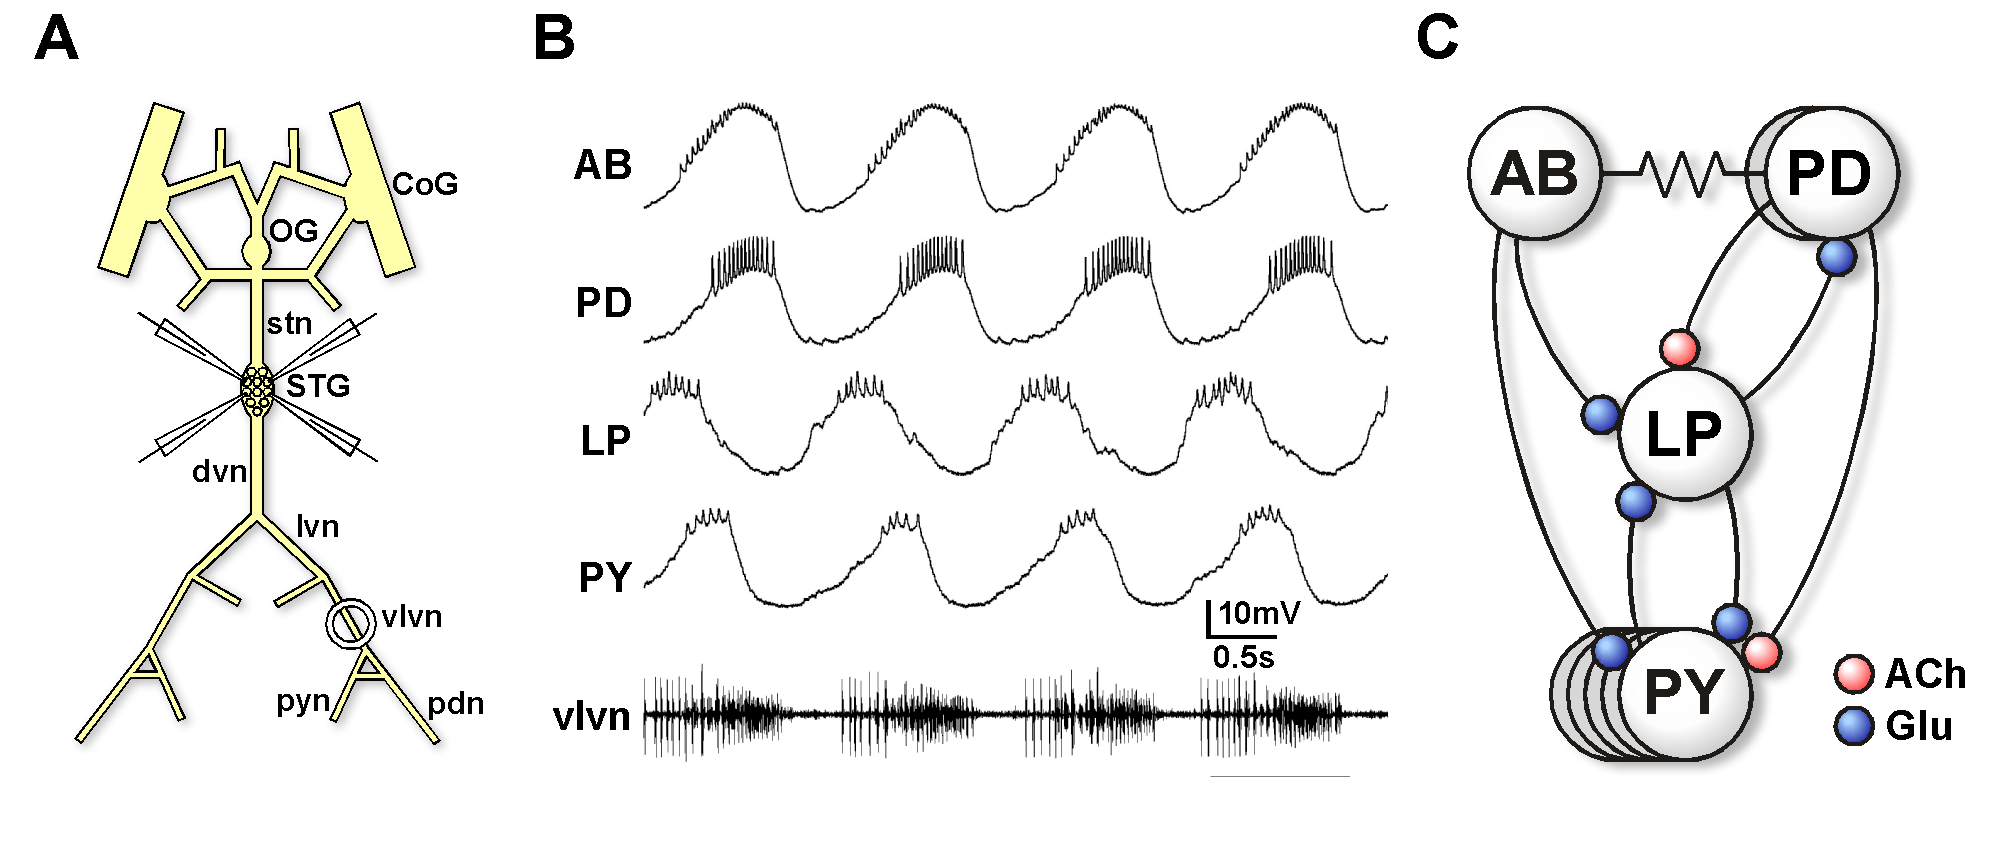
\includegraphics[width=1.0\linewidth]{gfx/PyloricRhythm}
	\caption[The stomatogastric ganglion]{The stomatogastric ganglion. (\textsc{A}) Diagram of the \acs{STNS} showing the ganglia (capitals) and the major nerves (lowercase). (\textsc{B}) Intracellular recordings from four cells in the pyloric circuit of the \acs{STG}. The fifth trace shows extracellular \textit{vlvn} nerve recording, which contains potentials from the above cells. (\textsc{C}) Circuit diagram showing synaptic connectivity in the pyloric circuit. Resistor symbols indicate electrical synapses. \textsc{ACh} are acetylcholinergic and \textsc{Glu} are glutamateric synapses, where balls indicate post-synaptic targets\autocite{NusbaumMichaelP.Functionalconsequencesneuropeptide2017}.}
	\label{fig:pyloricrhythm}
\end{figure}


\acs{STG} neurons have large somata (typically 50-100 microns across) and complex dendritic morphology\autocite{OtopalikSloppymorphologicaltuning2017,CuntzOnerulegrow2010}. While these cells possess long axons which contribute to descending nerves, much of the arborization consists of neurites which tangle extensively in the neuropil. This wiring follows a space-filling mechanism. Despite this tangled morphology, \acs{STG} neurons are electronically compact. Gradations in reversal (Nernst) potential as a function of path distance from the soma maintain signal amplitude near and far from zones of integration\autocite{OtopalikSloppymorphologicaltuning2017}. Therefore, the circuit relies on intrinsic and synaptic properties instead of morphological tuning to produce network activity.

Robustness to mechanical insult permits dissection and electrophysiological recording \textit{in-vitro}. The fictive motor patterns produced by the \acs{STG} survive for at least 24 hours without incubation and are representative of both the activity of the circuit \textit{in-vivo} and the motor output\autocite{HamoodConsequencesacutelongterm2015}. Additionally, since most synaptic connections in the \acs{STG} occur between motor neurons, the circuit can be isolated from descending interneurons\autocite{HamoodQuantitativeReevaluationEffects2015,GoldmanGlobalStructureRobustness2001,HaddadCircuitrobustnesstemperature2017}.  Decentralization by severing the \textit{stn}, the descending nerve which connects the \acsp{CoG} and \acs{OG} to the \acs{STG}, removes descending neuromodulation.

\begin{figure}[h]
	\centering
	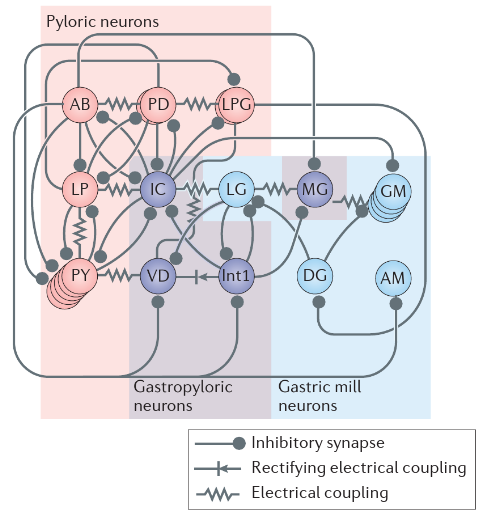
\includegraphics[width=1\linewidth]{gfx/NusbaumMarder2017.png}
	\caption[Circuit diagram of the STG]{Circuit diagram of the stomatogastric ganglion (\acs{STG}). Circles are neurons, resistor symbols are electrical synapses, balls indicate post-synaptic inhibitory targets.\autocite{NusbaumMichaelP.Functionalconsequencesneuropeptide2017}.}
	\label{fig:circuitdiagram}
\end{figure}

\FloatBarrier


\section{The Pyloric Rhythm}
The pyloric rhythm is a triphasic motor pattern almost always continuously expressed in the healthy crustacean\autocite{ClemensLongtermexpressiontwo1998,RezerExpressioncrustaceanpyloric1983}. The frequency of the rhythmic behavior may vary over $[0.5, 2.5]$ Hz, but the burst order, phase relationships, and duty cycle are maintained in healthy animals\autocite{MarderUnderstandingCircuitDynamics2007}. The canonical pyloric rhythm consists of bursts of action potentials in the pyloric dilator (\acs{PD}) neurons, followed by bursts in the lateral pyloric (\acs{LP}) neuron, and finally by bursts in the pyloric (\acs{PY}) neurons. The inferior cardiac (\acs{IC}) neuron fires often with the (\acs{LP}) neuron and the ventricular dilator (\acs{VD}) neuron fires frequently with the PY neurons\autocite{Harris-WarrickDynamicBiologicalNetworks1992}. The anterior burster (\acs{AB}) interneuron projects through the stomatogastric nerve to the \acsp{CoG} and is electrically coupled to the twin \acs{PD} neurons. 

In normal pyloric activity, the \acs{AB} neuron intrinsically oscillates. The \acs{PD} neurons, electrically coupled to \acs{AB}, burst in phase. The \acs{AB} and \acs{PD} cells inhibit \acs{LP} and \acs{PY}, which both burst during \acs{PD} interphase. \acs{LP} rebounds from inhibition faster than \acs{PY} and bursts first. \acs{LP} and \acs{PY} are in a phase-antiphase ’half-center’ oscillator regime of mutual inhibition (\autoref{fig:pyloricrhythm}). \acs{PY} neurons rebound and inhibit \acs{LP} to terminate bursting in the coupled cell\autocite{MarderUnderstandingCircuitDynamics2007,HooperModulationlobsterpyloric1987,Harris-WarrickDynamicBiologicalNetworks1992}. In this regime, \acs{AB} is considered the intrinsic pacemaker and \acs{AB}-\acs{PD} the pacemaker kernel. Selective photo-inactivation of cell types and glutamate-blocker experiments show that \acs{AB} reliably maintains oscillations while decoupled\autocite{SelverstonCrustaceanStomatogastricSystem1987}. The phaselocking of \acs{LP} and \acs{PY} during \acs{PD} interphase is dependent on the intrinsic and synaptic characteristics of the network. 

The pyloric rhythm is robust to perturbation. The circuit is most stable under physiological conditions (11 deg. C with descending neuromodulatory input), however the STG can maintain the phase differences characteristic of pyloric rhythmicity at temperatures up to 31 deg. C and under long-term decentralization\autocite{HaddadCircuitrobustnesstemperature2017,TangRobustnessrhythmiccircuit2012,HamoodConsequencesacutelongterm2015,GoldmanGlobalStructureRobustness2001}.

While the pyloric rhythm is robust to environmental perturbation, it is also susceptible to neuromodulation, allowing for flexibility in network output while maintaining stability. Neuromodulators are released into the neuropil as a consequence of sensation in the animal or descending modulatory projections from the \acsp{CoG} and \acs{OG}\autocite{MarderNeuromodulationNeuronalCircuits2012,JohnsonAminemodulationglutamate1997,Nusbaumsmallsystemsapproachmotor2002,MarderCentralpatterngenerators2001,Nusbaumrolescotransmissionneural2001}.

 
\begin{figure}[h]
	\centering
	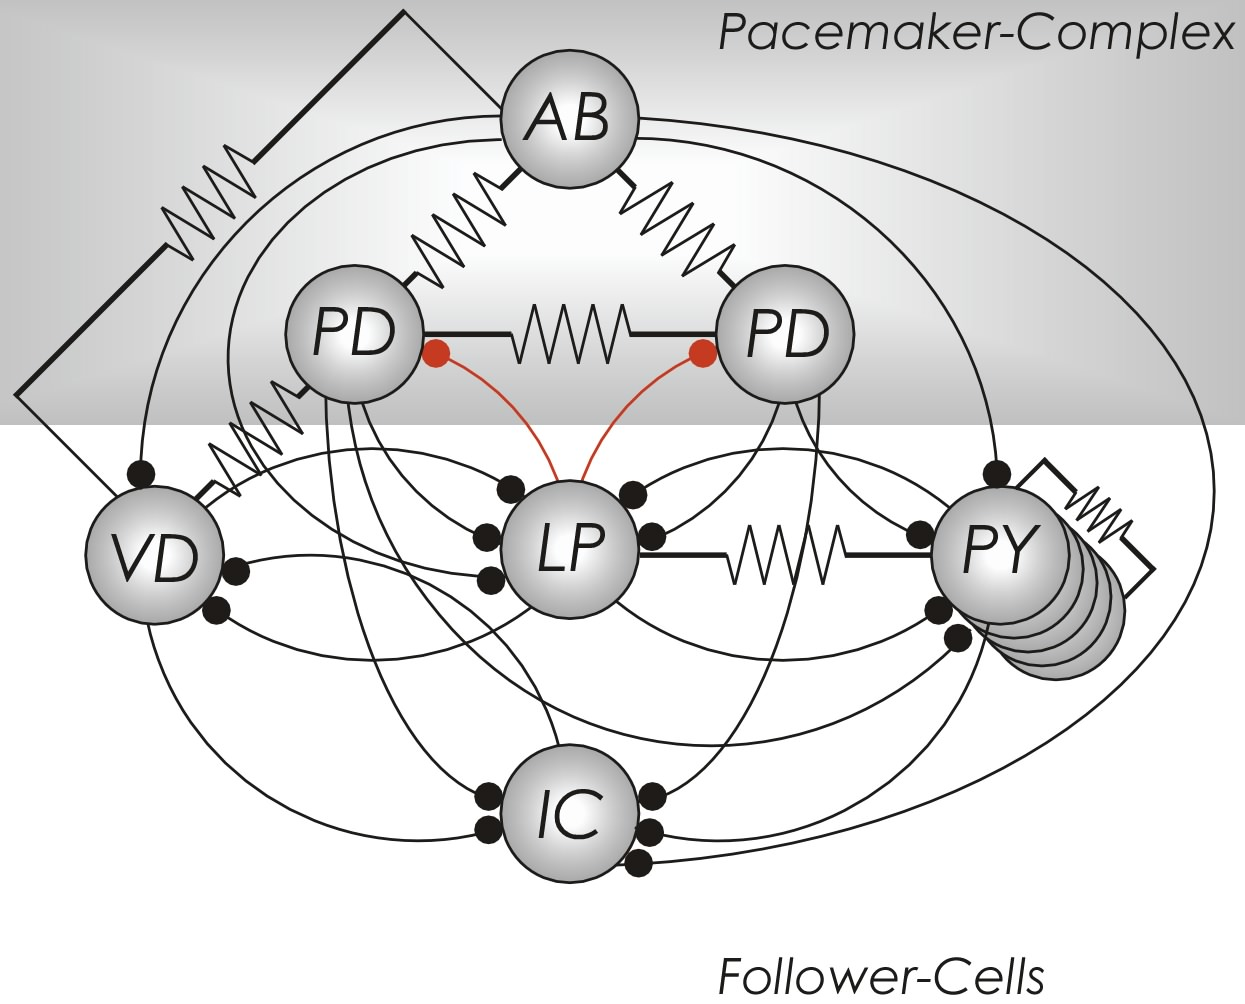
\includegraphics[width=1\linewidth]{gfx/PyloricCircuit}
	\caption[Circuit diagram of the pyloric circuit]{Circuit diagram of the pyloric circuit. Resistor symbols represent electrical synapses, dots represent inhbitory synapses. \acs{AB} and \acs{PD} form the pacemaker kernel.}
	\label{fig:pyloriccircuit}
\end{figure}

The \acs{STG} is multiply-modulated. The pericardial organ and other neurosecretory organs secrete neuromodulators into the neuropil which colocalize in specific neurons. In addition, many hormones circulating in the hemolymph can also act as neuromodulators in the \acs{STG}\autocite{MarderNeuromodulationNeuronalCircuits2012,NusbaumMichaelP.Functionalconsequencesneuropeptide2017,BlitzDifferentProctolinNeurons1999}.

In general, neuromodulators enhance the flexibility of neuronal networks. In one such method, neuromodulators activate a new current \acs{IMI}, a  fast, non-inactivating, voltage-gated inward current which predominately activates between -40 mV and -20 mV\autocite{GolowaschIoniccurrentslateral1992,GolowaschProctolinactivatesinward1992}.

All cells in the pyloric circuit are capable of activating \acs{IMI} through modulatory action, though they vary in its response. Differential receptor expression leads to variability and flexibility in cellular and network response to modulatory chemicals\autocite{SchulzVariablechannelexpression2006,OLearyCorrelationsionchannel2013}.

Application of red-pigment concentrating hormone (\acs{RPCH}) to the \acs{STG} increases the frequency and amplitude of slow-wave oscillations in the pyloric circuit, while phase relationships are maintained\autocite{NusbaumNeuronalRoleCrustacean1988} (\autoref{fig:rosenbaum2}, P. Rosenbaum, unpublished). Thus, the nerves which innervate the pylorus transmit the same patterned activity at the desired frequency, maintaining muscle tonus. 

\begin{figure}[h]
	\centering
	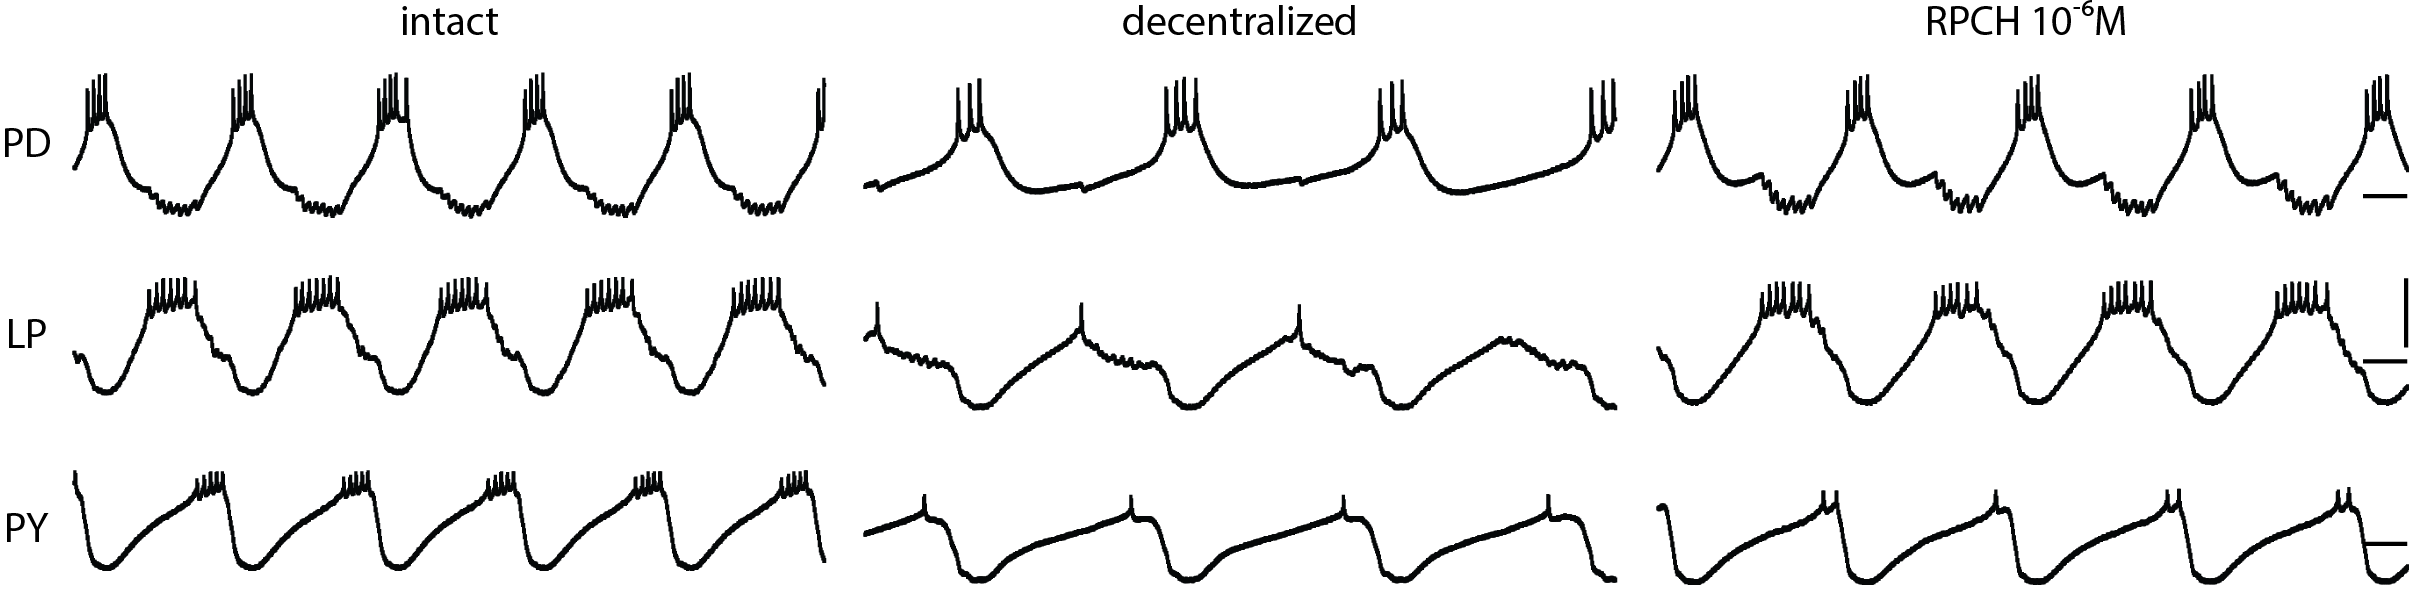
\includegraphics[width=1\linewidth]{gfx/Rosenbaum2}
	\caption[Pyloric Rhythms in \acs{RPCH}]{Pyloric rhythms in \acs{RPCH}. Traces on the left show a regular pyloric rhythm in the intact \acs{STNS}. Intracellular recordings of \acs{PD}, \acs{LP}, and \acs{PY} and an extracellular recording of the \textit{lvn} (lateral ventricular nerve) show the coordinated, triphasic rhythm. The intact rhythm has a frequency of about 1 Hz. Following decentralization (middle trace) the rhythm frequency and spikes per burst in all neurons decreased. After application of 1 $\mu \mathrm{M}$ \acs{RPCH}, the rhythm sped up and spikes per burst increased. Horizontal scale bars denote the membrane potential at -50 mV, vertical scale bars mark 20 mV (P. Rosenbaum, unpublished).}
	\label{fig:rosenbaum2}
\end{figure}

Three models of \acs{IMI} were examined. The first, published in Sharp \textit{et al.}, mimics proctolin in \acs{AB} neurons of \textit{C. borealis} using dynamic clamp\autocite{SharpDynamicclampcomputergenerated1993}. The characteristic increase in burst frequency and slow-wave amplitude under \acs{IMI} is shown in \autoref{fig:sharp2}.

\begin{figure}[h]
	\centering
	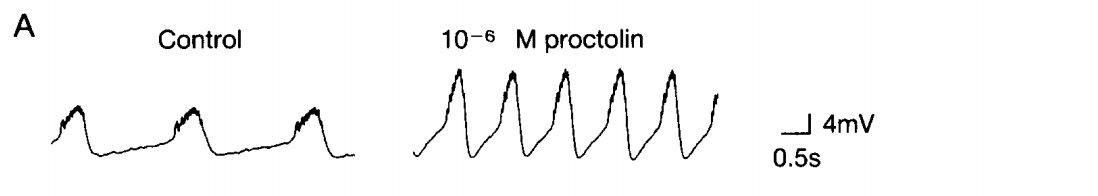
\includegraphics[width=1\linewidth]{gfx/Sharp2}
	\caption[Proctolin on AB neurons]{Proctolin increases amplitude and frequency of \acs{AB} oscillations. Intracellular recording from a lobster \acs{AB} neuron in control saline and 1 $\mu \mathrm{M}$ proctolin.\autocite{SharpDynamicclampcomputergenerated1993}.}
	\label{fig:sharp2}
\end{figure}


Swensen \& Marder fit current-voltage and dosage-response curves to proctolin in \acs{PD} and \acs{PY} neurons\autocite{SwensenMultiplepeptidesconverge2000,SwensenModulatorsconvergentcellular2001}. The \acs{STG} was decentralized from descending neuromodulatory inputs with sucrose block and artificial proctolin current was added via dynamic clamp, based on IV curves.

Soto-Trevi\~no \textit{et al.} developed a model of the pacemaker kernel based on recordings in spiny lobsters\autocite{Soto-TrevinoComputationalmodelelectrically2005}. Neuromodulatory inputs into the AB neuron were modeled by \acs{IMI}. The current was fit to the model, rather than to biological data. The parameters of the current satisfied the constraints that the model would mimic decentralized behavior without the current, and control behavior with the current.

\FloatBarrier

\section{Neurodynamics}
Analysis of high-dimensional conductance-based models form the backbone of this thesis. Each neuron is considered to consist of compartments, each with membrane properties and a collection of ionic and synaptic currents\autocite{AbbottAnalysisNeuronModels1993,Liumodelneuronactivitydependent1998}. The membrane potential $V_m$ of a compartment evolves according to the Hodgkin-Huxley formalism, which envisions excitable membranes as capacitors with variable resistors in parallel\autocite{Hodgkincomponentsmembraneconductance1952}. The membrane potential evolves over time as a function of the sum of the transmembrane currents. This is described by the conservation of current equation for a capacitative membrane.

\begin{equation} \label{eq:voltage}
	C_m \frac{\mathrm{d}V_m}{\mathrm{d}t} = - \sum_i I_i
\end{equation}

where $C_m$ is the membrane capacitance and $I_i$ each current. Each current is described as non-Ohmic with conductance $g$.

\begin{align}
	I_i(V_m) =&\ g_i(V_m)(V_m-E_i) \\
	g_i(V_m) =&\ \bar{g}_i m_i^{p_i} h_i^{q_i}
\end{align}

where

\begin{tabular}{ll}
	$\bar{g}$    & maximal conductance \\
	$m$     	 & activation gating variable \\
	$h$          & inactivation gating variable \\
	$p,q$        & integer exponents \\
	$E$          & reversal (Nernst) potential \\
\end{tabular}

The gating variables $m$ and $h$ are bounded in $[0, 1]$ so that the effective conductance $g_i(V_m)$ from the $i^{th}$ conductance lies between zero and the maximal conductance. When $m=0$, no channels of that conductance are open; when $h = 0$, all channels of that conductance are inactivated.

The gating variables evolve with time

\begin{equation}
	\tau_x(V_m) \frac{\mathrm{d}x}{\mathrm{d}t} = x_{\infty}(V_m) - x
\end{equation}

where

\begin{tabular}{ll}
	$x$   		 & $=(m,h)$ \\
	$\tau_x$  	 & time constant \\
	$x_\infty$   & steady-state function
\end{tabular}

Each conductance has characteristic steady-state and time constant functions which describe its role in the neurodynamics. The steady-states generally take the form of Boltzmann functions, fit from experiment\autocite{TurrigianoSelectiveregulationcurrent1995}.

In most models, reversal potentials for all ions excepting $\mathrm{Ca}^{2+}$ are fixed to constants, owing to the large ion concentration inside and outside the cell with respect to the number of ions fluxed\autocite{DayanTheoreticalNeuroscience2001,Liumodelneuronactivitydependent1998}. Intracellular calcium concentration changes as a function of calcium buffering rate and calcium currents. 

\begin{equation} \label{eq:calcium}
	\tau_{Ca} \frac{\mathrm{d} \left[ Ca^{2+} \right]}{\mathrm{d}t} = \left[ Ca^{2+} \right]_\infty - \left[ Ca^{2+} \right]
\end{equation}

The steady-state function $\left[ Ca^{2+} \right]_\infty (I_{Ca})$ is a function of the calcium currents; the actual calcium current lags with the time constant.

\begin{equation}
	\left[ Ca^{2+} \right]_\infty (I_{Ca}) = - f \sum_{Ca} I_{Ca} + \left[ Ca^{2+} \right]_0
\end{equation}

In this context, $f$ is a buffering coefficient which translates the calcium flux (in units of current per area) into a steady-state concentration. $\left[ Ca^{2+} \right]_0$ represents the equilibrium intracellular calcium concentration. 
 
Similarly, membrane capacitance is generally taken to be constant, following seminal work by Huxley, showing that the specific membrane capacitance varies on $[9, 15]\ \mathrm{nF/mm^2}$. In models, the membrane capacitance is typically set to unity\autocite{Liumodelneuronactivitydependent1998,PrinzAlternativehandtuningconductancebased2003,PrinzSimilarnetworkactivity2004,OLearyCellTypesNetwork2014}.

From the complex nonlinear interplay of several conductances, neuronal dynamics emerge.

\section{Modeling the Stomatogastric Ganglion}
The steady-state and time constant functions are based on experimental data by \autocite{TurrigianoSelectiveregulationcurrent1995}. IV curves and current traces in voltage clamp were produced. Steady-states were fit to Boltzmann functions.

\[ x_\infty(V_m) = \frac{1}{1 + \exp \left( \frac{V+V_{th}}{V_\sigma} \right)} \]

where $V_{th}$ is the half-potential (i.e. $x_\infty(V_{th}) = 0.5$) and $V_\sigma$ describes the width of the distribution. Timescales were extracted from the current traces, and generally take the form of Hill functions.

Neurons in the \acs{STG} are isopotential. Projections in the \acs{STG} operate on a space-filling mechanism, resulting in a dense neuropil\autocite{CuntzOnerulegrow2010}. Effective reversal potentials vary by path length from soma, so that \acs{STG} neurons are electrotonically compact\autocite{OtopalikSloppymorphologicaltuning2017}. Response in the soma is comparable to elsewhere, meaning that the cells are isopotential. 

Strogatz explains that, ``No insight is gained if the model is as perplexing as the phenomena it is supposed to describe,"\autocite{StrogatzSyncEmergingScience2003}. To this end, conductance-based models of the \acs{STG} have strived for verisimilitude only so much as to encompass te burst characteristics, phase relationships, and other neurocomputational properties of the circuit. Since \acs{STG} neurons are electronically compact, single-compartment (isopotential) models are suitable for representing time-correlated circuit output\autocite{AbbottAnalysisNeuronModels1993,PrinzAlternativehandtuningconductancebased2003,PrinzComputationalapproachesneuronal2010}. In real cells, action potentials begin in the spike-initiation zone, so that spikes appear attenuated in somatic recordings. This can be rectified in computational models by creating two-compartment models, increasing realism at the expense of increasing the complexity\autocite{Soto-TrevinoComputationalmodelelectrically2005}.

Single-compartment conductance-based models demonstrate that diverse sets of maximal conductances can produce spiking activity. While the set of points in conductance space which elicit spiking behavior is not ergodic, the spiking subspace is much larger than initially expected\autocite{PrinzAlternativehandtuningconductancebased2003}. In three-cell networks (\acs{AB}-\acs{PD}, \acs{LP}, \acs{PY}), simulations elicited similar network activity from disparate network parameters, showing the theoretical possibility of significant network degeneracy\autocite{PrinzSimilarnetworkactivity2004}. These theoretical intuitions are supported by electrophysiology and \textsc{mRNA} assays, which demonstrate highly variable animal-to-animal \textsc{mRNA} and channel expression\autocite{SchulzVariablechannelexpression2006,GoaillardFunctionalconsequencesanimaltoanimal2009,HamoodAnimaltoanimalvariabilityneuromodulation2014}.

\begin{figure}[h]
	\centering
	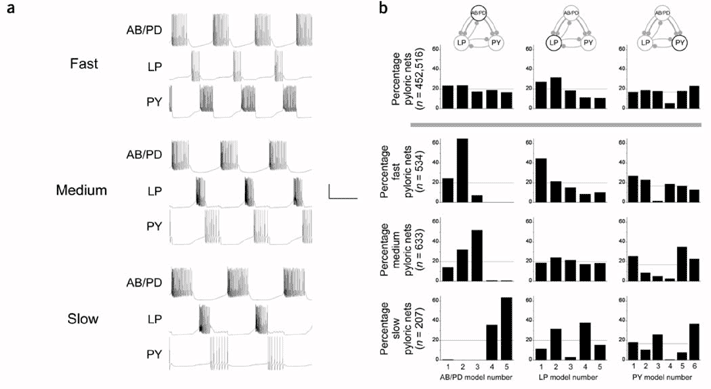
\includegraphics[width=1.0\linewidth]{gfx/Prinz6}
	\caption[Network degeneracy in model pyloric circuits.]{Network degeneracy in model pyloric circuits. (a) Voltage traces from simulated pyloric networks in fast, medium, and slow burst-frequency ranges. Scale bars, 1 s and 50 mV. (b) Percentages of pyloric networks that contain a given \acs{AB}-\acs{PD} model neuron (left), \acs{LP} model neuron (middle), or \acs{PY} model neuron (right). Top row, distributions for all pyloric networks; bottom rows, distributions for fast, medium and slow pyloric networks\autocite{PrinzSimilarnetworkactivity2004}.}
	\label{fig:prinz6}
\end{figure}

It has been demonstrated that there are many ways to produce stable, predictable output in models, as in animals, but these models have not been tested in response to modulation. Neuromodulation is a key way by which a neuronal circuit can be robust to unwelcome perturbation yet still respond with specialized activity when modulated. Network degeneracy comes secondary to this biological necessity.




\cleardoublepage
\ctparttext{You can put some informational part preamble text here.
Illo principalmente su nos. Non message \emph{occidental} angloromanic
da. Debitas effortio simplificate sia se, auxiliar summarios da que,
se avantiate publicationes via. Pan in terra summarios, capital
interlingua se que. Al via multo esser specimen, campo responder que
da. Le usate medical addresses pro, europa origine sanctificate nos se.}
\part{The Showcase}\label{pt:showcase}
%*****************************************
\chapter{Methods}\label{ch:methods}
%*****************************************
For much of this thesis, single-compartment model neurons with Hodgkin-Huxley type membrane currents and an intracellular calcium buffer were used\autocite{HodgkinMeasurementcurrentvoltagerelations1952, Hodgkincomponentsmembraneconductance1952, Hodgkinquantitativedescriptionmembrane1952}. Similar models have been described previously\autocite{Liumodelneuronactivitydependent1998, PrinzAlternativehandtuningconductancebased2003, PrinzSimilarnetworkactivity2004, SoofiPhasemaintenancerhythmic2014}. The membrane currents are based on experiments on \textit{Homarus} neurons\autocite{TurrigianoSelectiveregulationcurrent1995}. 

Briefly, the currents consist of a \ac{INa}, a \ac{ICaT}, a \ac{ICaS}, a \ac{IA}, a \ac{IKCa}, a \ac{IKd}, a \ac{IH}, and a \ac{Ileak}.

\section{Model Parameters}
Model parameters were adapted from \autocite{PrinzAlternativehandtuningconductancebased2003, PrinzSimilarnetworkactivity2004}

\begin{figure}[h]
	\centering
	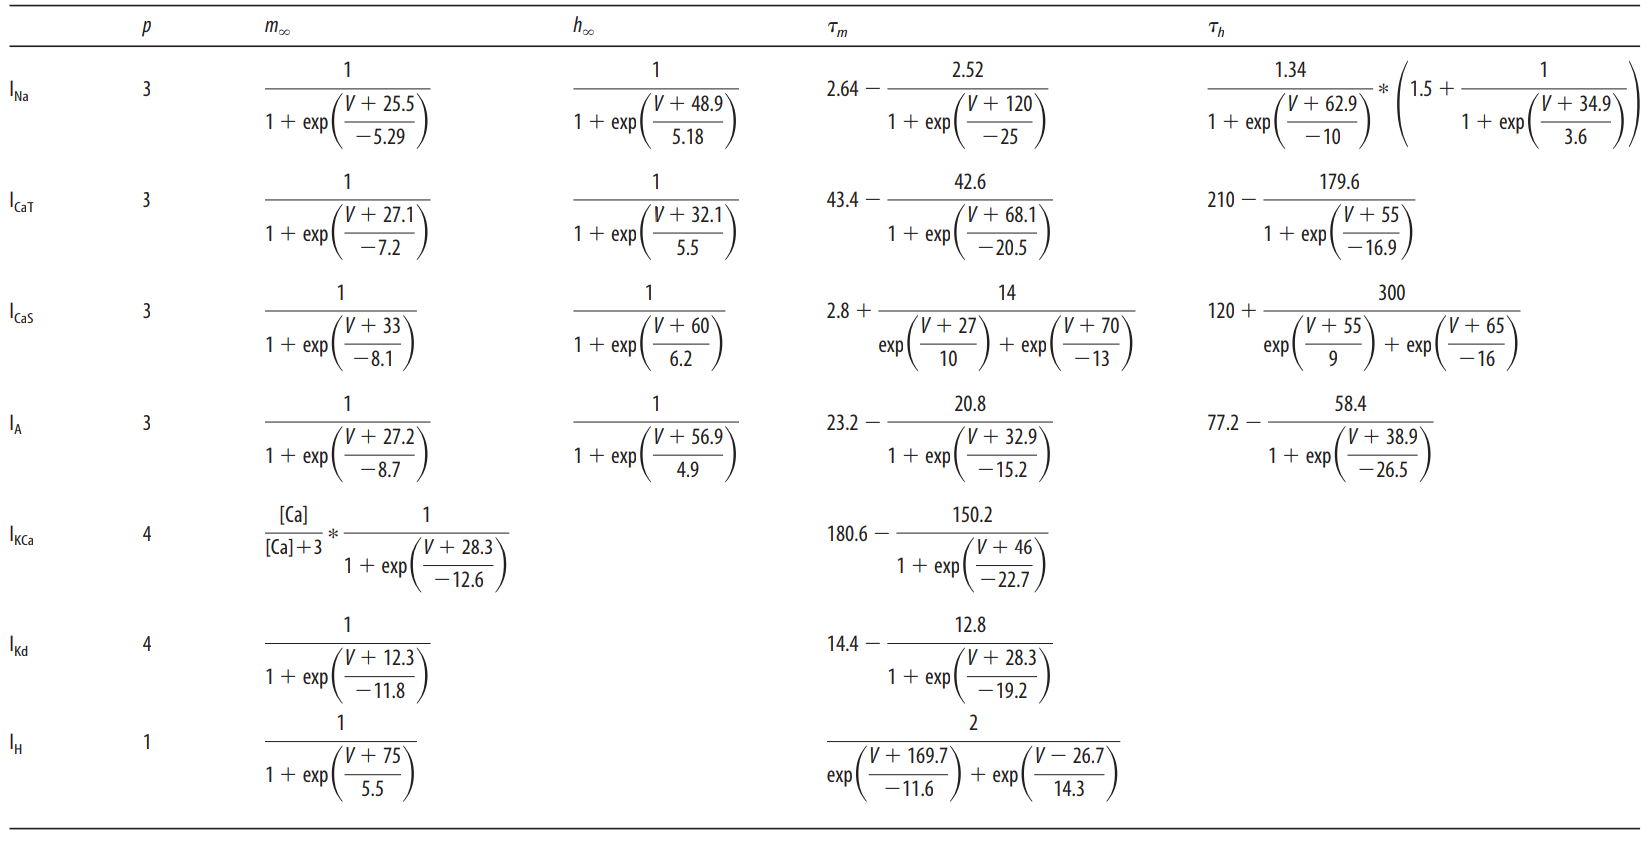
\includegraphics[width=1.0\linewidth]{gfx/VoltageDependence}
	\caption[Voltage dependence for model currents]{Voltage dependence of model currents. $V$ is the membrane potential in mV; $[Ca]$, the intracellular calcium concentration in mM. Absences in the table indicate non-inactivating currents (e.g. $h = 1 ~\forall~ V$).}
	\label{fig:voltagedependence}
\end{figure}

%\begin{table}[h]
%	\myfloatalign
%	\begin{tabularx}{\textwidth}{cccccc} \toprule
%		& p & $m_\infty$ & $h_\infty$ & $\tau_m$ & $\tau_h$ \\ \midrule
%		\acs{INa} & 3 & $ \frac{1}{1 + \exp \left( \frac{V + 25.5}{-5.29} \right)} $ & $ \frac{1}{1 + \exp \left( \frac{V + 48.9}{5.18} \right)} $ & $ 2.64 - \frac{2.52}{1 + \exp \left( \frac{V + 120}{-25} \right)} $ & $ \frac{1.34}{1 + \exp \left( \frac{V + 62.9}{-10} \right)} \left( 1.5 + \frac{1}{1 + \exp \left( \frac{V + 34.9}{3.6} \right)} \right) $ \\ 
%	\end{tabularx}
%	\caption[Reversal potentials for model currents]{Reversal potentials for model currents in mV. Calcium reversal potentials vary as a function of voltage and calcium.}  
%	\label{tab:voltagedependence}
%\end{table}

The reversal potentials determines the membrane potential at which a current begins fluxing ions in the opposite direction.

\begin{table}[h]
	\myfloatalign
	\begin{tabularx}{\textwidth}{ccccccccc} \toprule
		\tableheadline{Current} & \acs{INa} & \acs{ICaT} & \acs{ICaS} & \acs{IA} & \ac{IKCa} & \ac{IKd} & \ac{IH} & \ac{Ileak} \\ \midrule
		$E$ (mV) & 50 & * & * & -80 & -80 & -80 & -20 & -50 \\ \bottomrule
	\end{tabularx}
	\caption[Reversal potentials for model currents]{Reversal potentials for model currents in mV. Calcium reversal potentials vary as a function of voltage and calcium.}  
	\label{tab:reversalpotentials}
\end{table}

\FloatBarrier

The calcium reversal potential is computed from the Nernst potential\autocite{FreschiProctolinactivatesslow1989, GoldmanGlobalStructureRobustness2001}.

\begin{equation}
	E_{Ca} = \frac{RT}{zF} \ln \left( \frac{\left[ Ca^{2+} \right]_{ex}}{\left[ Ca^{2+} \right]_{in}} \right)
\end{equation}

where $\left[ Ca^{2+} \right]_{in}$ is the intracellular calcium concentration in $\mu\mathrm{M}$ and 

\begin{tabular}{ll}
	$\left[ Ca^{2+} \right]_{ex}$ & $=3~\mu\mathrm{M}$, extracellular calcium concentration \\
	$R$   		 & $=8.314~\mathrm{J\cdot mol/K}$, gas constant \\
	$T$  	 	 & $=284.15~\mathrm{K}$, temperature \\
	$z$   		 & $=2$, valence of calcium cation \\
	$F$ 		 & $=96485~\mathrm{C/mol}$, Faraday constant
\end{tabular}

The calcium concentration evolves with time (\autoref{eq:calcium}), where

\begin{tabular}{ll}
	$\tau_{Ca}$	 & $=200~\mathrm{ms}$, calcium buffering time constant \\
	$f$  	 	 & $=14.96~\mu\mathrm{M/nA}$, conversion factor
\end{tabular}

The conversion factor translates calcium currents into a rate of intracellular calcium flux\autocite{PrinzAlternativehandtuningconductancebased2003,Liumodelneuronactivitydependent1998}. The factor depends on the ratio of the surface area of the cell to the volume in which the calcium concentration is measured. The buffering zone is taken to be a narrow cylindrical shell just inside the membrane with a diameter of 50 microns and length 400 microns. Finally, the voltage evolves (\autoref{eq:voltage}) with membrane capacitance $C_m = 10~\mathrm{nF/mm^2}$ where the surface area of the cell is $0.0628~\mathrm{mm^2}$\autocite{Hodgkinquantitativedescriptionmembrane1952,Liumodelneuronactivitydependent1998}.

Synapses were modeled as non-inactivating currents according to a standard model\autocite{AbbottModelingSmallNetworks1998}. The synaptic current is

\begin{equation}
	I_{syn} = g_{syn} s (V_{post} - E_{syn})
\end{equation}

where $V_{post}$ is the membrane potential of the postsynaptic neuron and $E_{syn}$ is the reversal potential of the synapse. The synaptic gating variable $s$ evolves with time.

\begin{align}
	\frac{\mathrm{d}s}{\mathrm{d}t} &=\ \frac{s_\infty (V_{pre}) - s}{\tau_{syn}} \\
	s_\infty (V_{pre}) &=\ \frac{1}{1 + \exp \left( \frac{V + V_{th}}{-V_\sigma} \right)} \\
	\tau_{syn} &=\  \tau_d \left( 1 - s_\infty(V_{pre}) \right)
\end{align}

where

\begin{tabular}{ll}
	$V_{pre}$	& membrane potential of the presynaptic neuron \\
	$V_{th}$ 	& half-potential of the synapse \\
	$V_\sigma$ 	& describes the slope of the activation curve \\
	$\tau_d$ 	& time constant for transmitter-receptor dissociation \\
\end{tabular}

\acs{AB}, \acs{LP}, and \acs{PY} are glutamatergic neurons whereas \acs{PD} is cholinergic.

\begin{table}[h]
	\myfloatalign
	\begin{tabularx}{\textwidth}{lcc} \toprule
		\tableheadline{Constant} & \tableheadline{Glutamatergic} & \tableheadline{Cholinergic} \\ \midrule
		$E$ (mV) & -70 & -80 \\
		$V_{th}$ (mV) & -35 & -35 \\
		$V_\sigma$ (mV) & 5 & 5 \\
		$\tau_d$ (ms) & 40 & 100 
	\end{tabularx}
	\caption[Constants for model synapses]{Constants for synaptic currents.}  
	\label{tab:synapses}
\end{table}

\section{Simulating Model Neurons} \label{sec:simulating}
Model neurons were simulated with a time step $\mathrm{d}t = 0.1~\mathrm{ms}$ using the exponential Euler method\autocite{DayanTheoreticalNeuroscience2001}. 

\begin{align} \label{eq:expeuler}
	V_m (t + \mathrm{d}t) =&\ V_\infty + (V_m (t) - V_\infty) \exp \left( -\frac{\mathrm{d}t}{\tau_V} \right) \\
	V_\infty =&\ \frac{ \sum_i g_i(V_m) E_i }{ \sum_i g_i(V_m) } \\
	\tau_V =&\ \frac{C_m}{ \sum_i g_i (V_m) }
\end{align}

This method is asymptotically stable, unlike linear Euler and much faster than higher order Runge-Kutta methods. Initial conditions were standardized as follows.

\begin{table}[h]
	\myfloatalign
	\begin{tabularx}{\textwidth}{cccc} \toprule
		$V_m$ & $\left[Ca^{2+}\right]_{in}$ & $m$ & $h$ \\ \midrule
		-65 & 0.02 & 0 & 1 \\
		\bottomrule
	\end{tabularx}
	\caption[Initial conditions]{Initial conditions for typical simulations. Voltage is in mV, calcium concentration is in $\mu$M.}  
	\label{tab:initialconditions}
\end{table}

Unless otherwise specified, the first 25\% of a simulation was discarded as transient.

\FloatBarrier

\section{The Prinz Database} \label{sec:prinzdatabase}
In order to characterize the solution space for single-compartment \acs{AB}-\acs{PD}-like models, all bursting neurons in the database described in Prinz \textit{et al.} were simulated. Since \acs{AB} neurons continue to oscillate in the presence of sodium channel blockers, \acs{AB}-like models were implemented without spike-producing \acs{INa} or \acs{ICaT} currents. A subset of Prinz models and optimized derivatives produce slow-wave voltage oscillations qualitatively similar to rectified sinusoids in the absence of these inward currents. The database expedited the search for candidate solutions to optimize.

The pyloric network models consist of three cellular compartments, \acs{AB}-\acs{PD}, \acs{LP}, and \acs{PY}. The intrinsic pacemaker \acs{AB} is strongly electrically coupled to the \acp{PD} and has been reduced to a single-compartment computational composite. All \acp{PY}, which are electrically coupled, have been reduced to a single \acs{PY} compartment.

\begin{figure}[h]
	\centering
	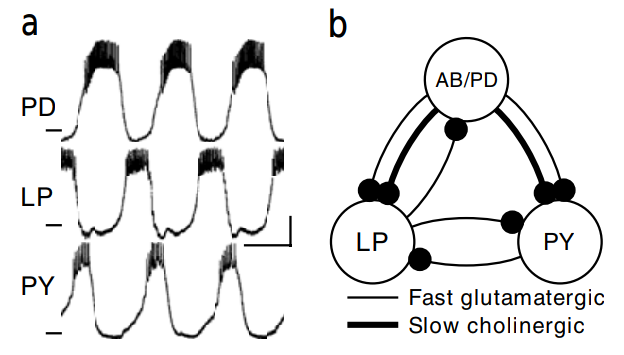
\includegraphics[width=1.0\linewidth]{gfx/prinz1}
	\caption[Pyloric network model architecture]{Biological pyloric rhythm and pyloric circuit model network. (\textsc{A}) Pyloric rhythm recorded from \textit{H. americanus} with intracellular electrodes. Scale bars, 1 s, and 10 mV; horizontal lines, -60 mV. (\textsc{B}) Schematic of a simplified version of the underlying circuit (\autoref{fig:circuitdiagram}). All synapses are inhibitory\autocite{PrinzSimilarnetworkactivity2004}.}
	\label{fig:prinz1}
\end{figure}

\FloatBarrier

\section{Modulatory Input} \label{sec:modulatoryinput}
Sharpe \textit{et al.} and Swensen \& Marder fit models of modulatory input current to experimental data. The Swensen model possesses a wider basin of activation without a sharp peak, and is based recordings from the \acs{PD} neuron. While both models fit proctolin data, \acs{RPCH} response more closely resembles the graded activation of Swensen \& Marder modulatory input.
\begin{table}[h]
	\myfloatalign
	\begin{tabularx}{\textwidth}{ccc} \toprule
		& Sharp \textit{et al.} & Swensen \& Marder \\ \midrule
		$V_{th}$ (mV) & -55 & -21 \\
		$V_\sigma$ (mV) & 5 & 8 \\
		$\tau_m$ (ms) & 6 & 6 \\
		$E$ (mV) & -10 & -22 \\
		\bottomrule
	\end{tabularx}
	\caption[Modulatory input current models]{Comparison of Sharp and Swensen modulatory input currents.}  
	\label{tab:sharpswensen}
\end{table}

\begin{figure}[h]
	\centering
	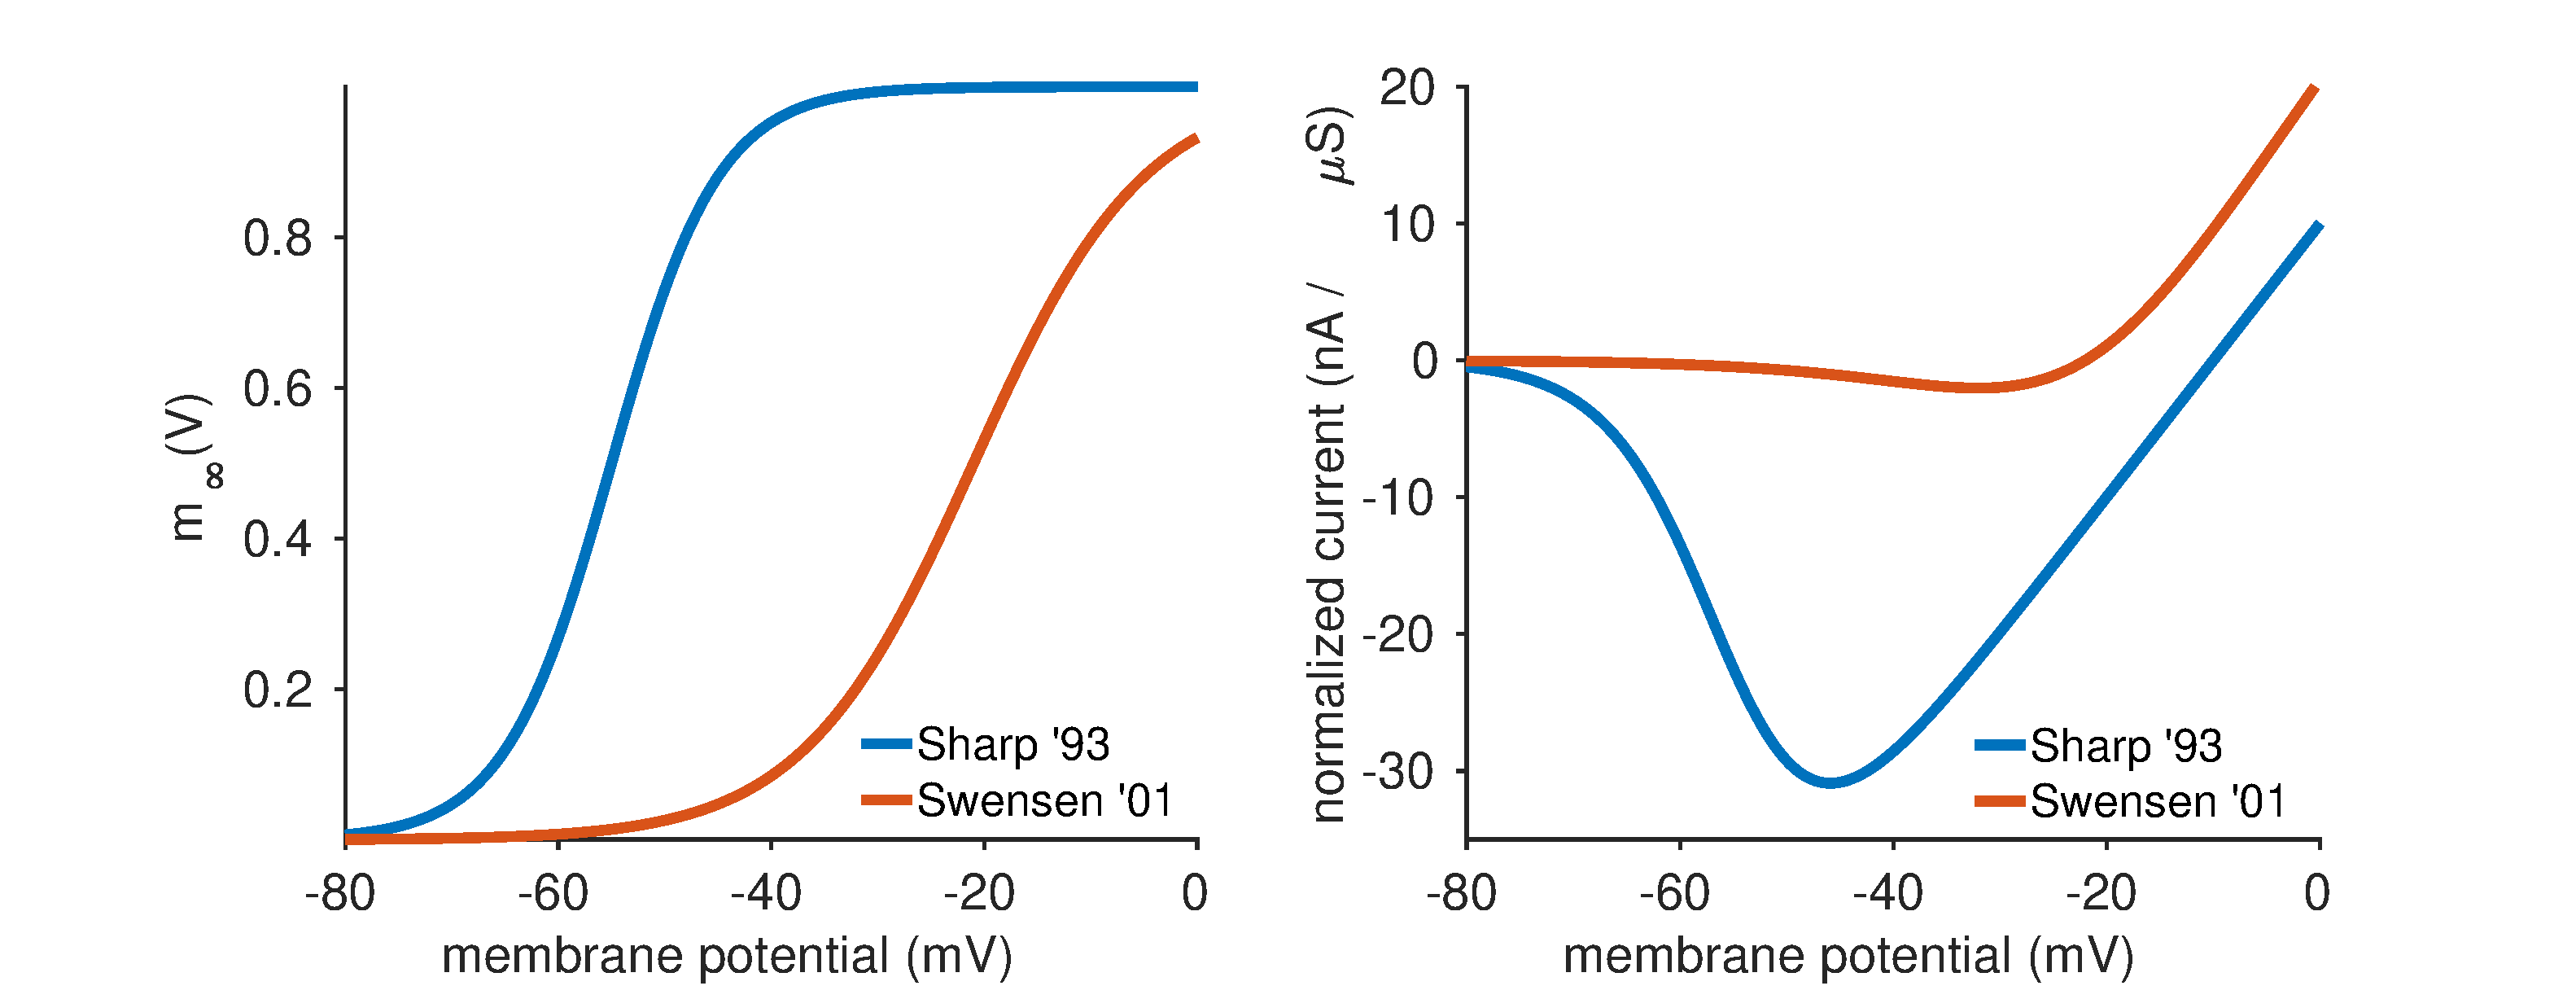
\includegraphics[width=1.0\linewidth]{gfx/SharpSwensen}
	\caption[Models of modulatory input current]{Models of modulatory input current. Sharp and Swensen modulatory input current are compared. The left-hand trace shows the activation gating variable steady-state as a function of membrane potential. The right-hand trace shows the IV curves for these model currents.}
	\label{fig:sharpswensen}
\end{figure}


\section{Model Implementation} \label{sec:modelimplementation}
In order to quickly simulate many models with varied parameters, we developed simulation software called \texttt{xolotl}. This fast single-compartment and multi-compartment simulator is written in \texttt{C++} with \texttt{MATLAB} wrappers. Designed with a focus on flexibility and speed, it can simulate single-compartment models, networks of these, and detailed multi-compartment models. This novel software has been developed by Srinivas Gorur-Shandilya and the author.

\graffito{\texttt{xolotl} is the Aztec god of lightning and death}

\texttt{xolotl} separates neurons into compartments, where each compartment and contained current is fully modular. Synapses link two compartments together. Compartments can contain any number of parameters and variables so that \texttt{xolotl} is readily adaptable to any number of simulation regimes. Since a main benefit of modeling is generating a large number of \textit{in-silico} experiments to support or generate hypotheses, \texttt{xolotl} objects can be passed through optimization protocols to develop sets of parameter values which satisfy arbitrary biological constraints. Many models can be generated which replicate biological behavior; since \acs{STG} neurons are degenerate with respect to maximal conductance density and conductance density can be assumed constant on non-homeostatic timescales, maximal conductances of intrinsic and synaptic currents serve as readily optimized parameters for single cell and network models.

Maximal conductances for intrinsic currents were bound by the interval $[0.1, 2000]~\mu \mathrm{S/mm^2}$ and synaptic conductances were bound by $[0.1,100]~\mu \mathrm{S/mm^2}$, keeping with Prinz \textit{et al.} Injected modulatory input current in dynamic clamp experiments typically lies in the range $[0,100]~\mathrm{nS}$. For this reason, maximal conductance density for \acs{IMI} was bounded by the interval $[0,1]~\mu \mathrm{S/mm^2}$ since

\begin{equation*}
	1~\mu \mathrm{S/mm^2} \times 0.0628~\mathrm{mm^2} \times \frac{1000~\mathrm{nS}}{1 \mu \mathrm{S}} = 62.8~\mathrm{nS}
\end{equation*}

Similarly, \citeauthor{SwensenModulatorsconvergentcellular2001} report the maximal steady-state current in \acs{PD} cells to be $-1.8~\mathrm{nA}$. A modeled maximal conductance of $1.0~\mu \mathrm{S/mm^2}$ would produce a current of $-2.0~\mathrm{nA}$. 

\subsection{Parameter Optimization} \label{sec:parameteroptimization}
The first step in any parameter optimization algorithm begins with the cost function $f: \mathbb{R}^n \rightarrow \mathbb{R}$. The function accepts a candidate solution in the form of a vector of real numbers and produces a real output, which represents the objective function value of the candidate solution. This process is necessary to objectively and unambiguously evaluate the fitness of a model by reducing the high-dimensional parameter set and the complicated non-analytical function which produces the resultant waveforms into a single real number. Optimization algorithms aim to discover candidate solutions which produce low costs, where a cost of zero signifies a model which fits the cost function perfectly. Since the \acs{STG} is highly degenerate in ion channel expression, maximal conductances are the targeted parameters. The solution space has been loosely characterized, producing a large number of parameter seeds to optimize.

\graffito{\texttt{procrustes} is a bandit of Greek mythology who forced his victims to fit into a bed, by stretching and amputating }

We built an optimization toolbox, \texttt{procrustes}, which optimizes any parameters passed to it based on an arbitrary cost function.  The interface serves as front-end for several parameter optimization algorithms used to develop models with desired metrics. Since application of \acs{RPCH} increases the burst frequency and maximum of the slow-wave oscillations in \acs{PD} and \acs{LP} cells, increases in these metrics over increasing modulatory input is strongly targeted. We tested \texttt{procrustes} with three parameter optimization algorithms: gradient descent, a genetic algorithm, and particle swarm optimization.

The simplest, gradient descent, is a first-order iterative algorithm in which candidate solutions take steps proportional to the gradient of the cost function at the current point. This method can readily be applied to high-dimensional spaces, though can be inefficient. Close to the minimum, gradient descent tends to ``zig-zag'' in parameter space. For a cost landscape with many local minima, many seeds with diverse parameter values must be used in order to effectively characterize possible solutions.

A genetic algorithm combines a gradient descent methods with stochastic ``mutation,'' in which solutions are combined or transformed to produce better ones. This has the advantage of more readily finding substantial local minima, but escaping from superficially fit solutions. Unfortunately, genetic algorithms are computationally expensive and suffer in problem domains with a complex cost landscape.

Particle swarm optimization relies on the generation of many candidate solutions (``particles'') which move in parameter space towards the best position of a particle in the swarm. Since the parameter space is widely sampled by the stochastically-generated particles, particle swarm optimization can efficiently handle complex cost landscapes and high-dimensional parameter spaces. Particle swarm optimization is especially effective in this case since solutions can be readily screened for non-bursting, non-triphasic activity and rejected by the swarm.

Regardless of algorithm, the greatest difficulty is almost always writing a sufficient cost function, which arrives at suitable solutions within appreciable time. Since no general technique exists for producing Lyapunov functions for ordinary differential equations; the cost function must be designed manually. A good cost function consistently produces models which satisfy the researcher's needs in efficient time. While the cost function must be ambiguous with respect to the constraints of optimization, the construction of the function and evaluation of resultant models is entirely arbitrary. \autoref{fig:procrustesexample} shows that optimization can arrive at suitable solutions in a short period of time, provided that an efficient and unambiguous cost function is implemented.

\begin{figure}[h]
	\centering
	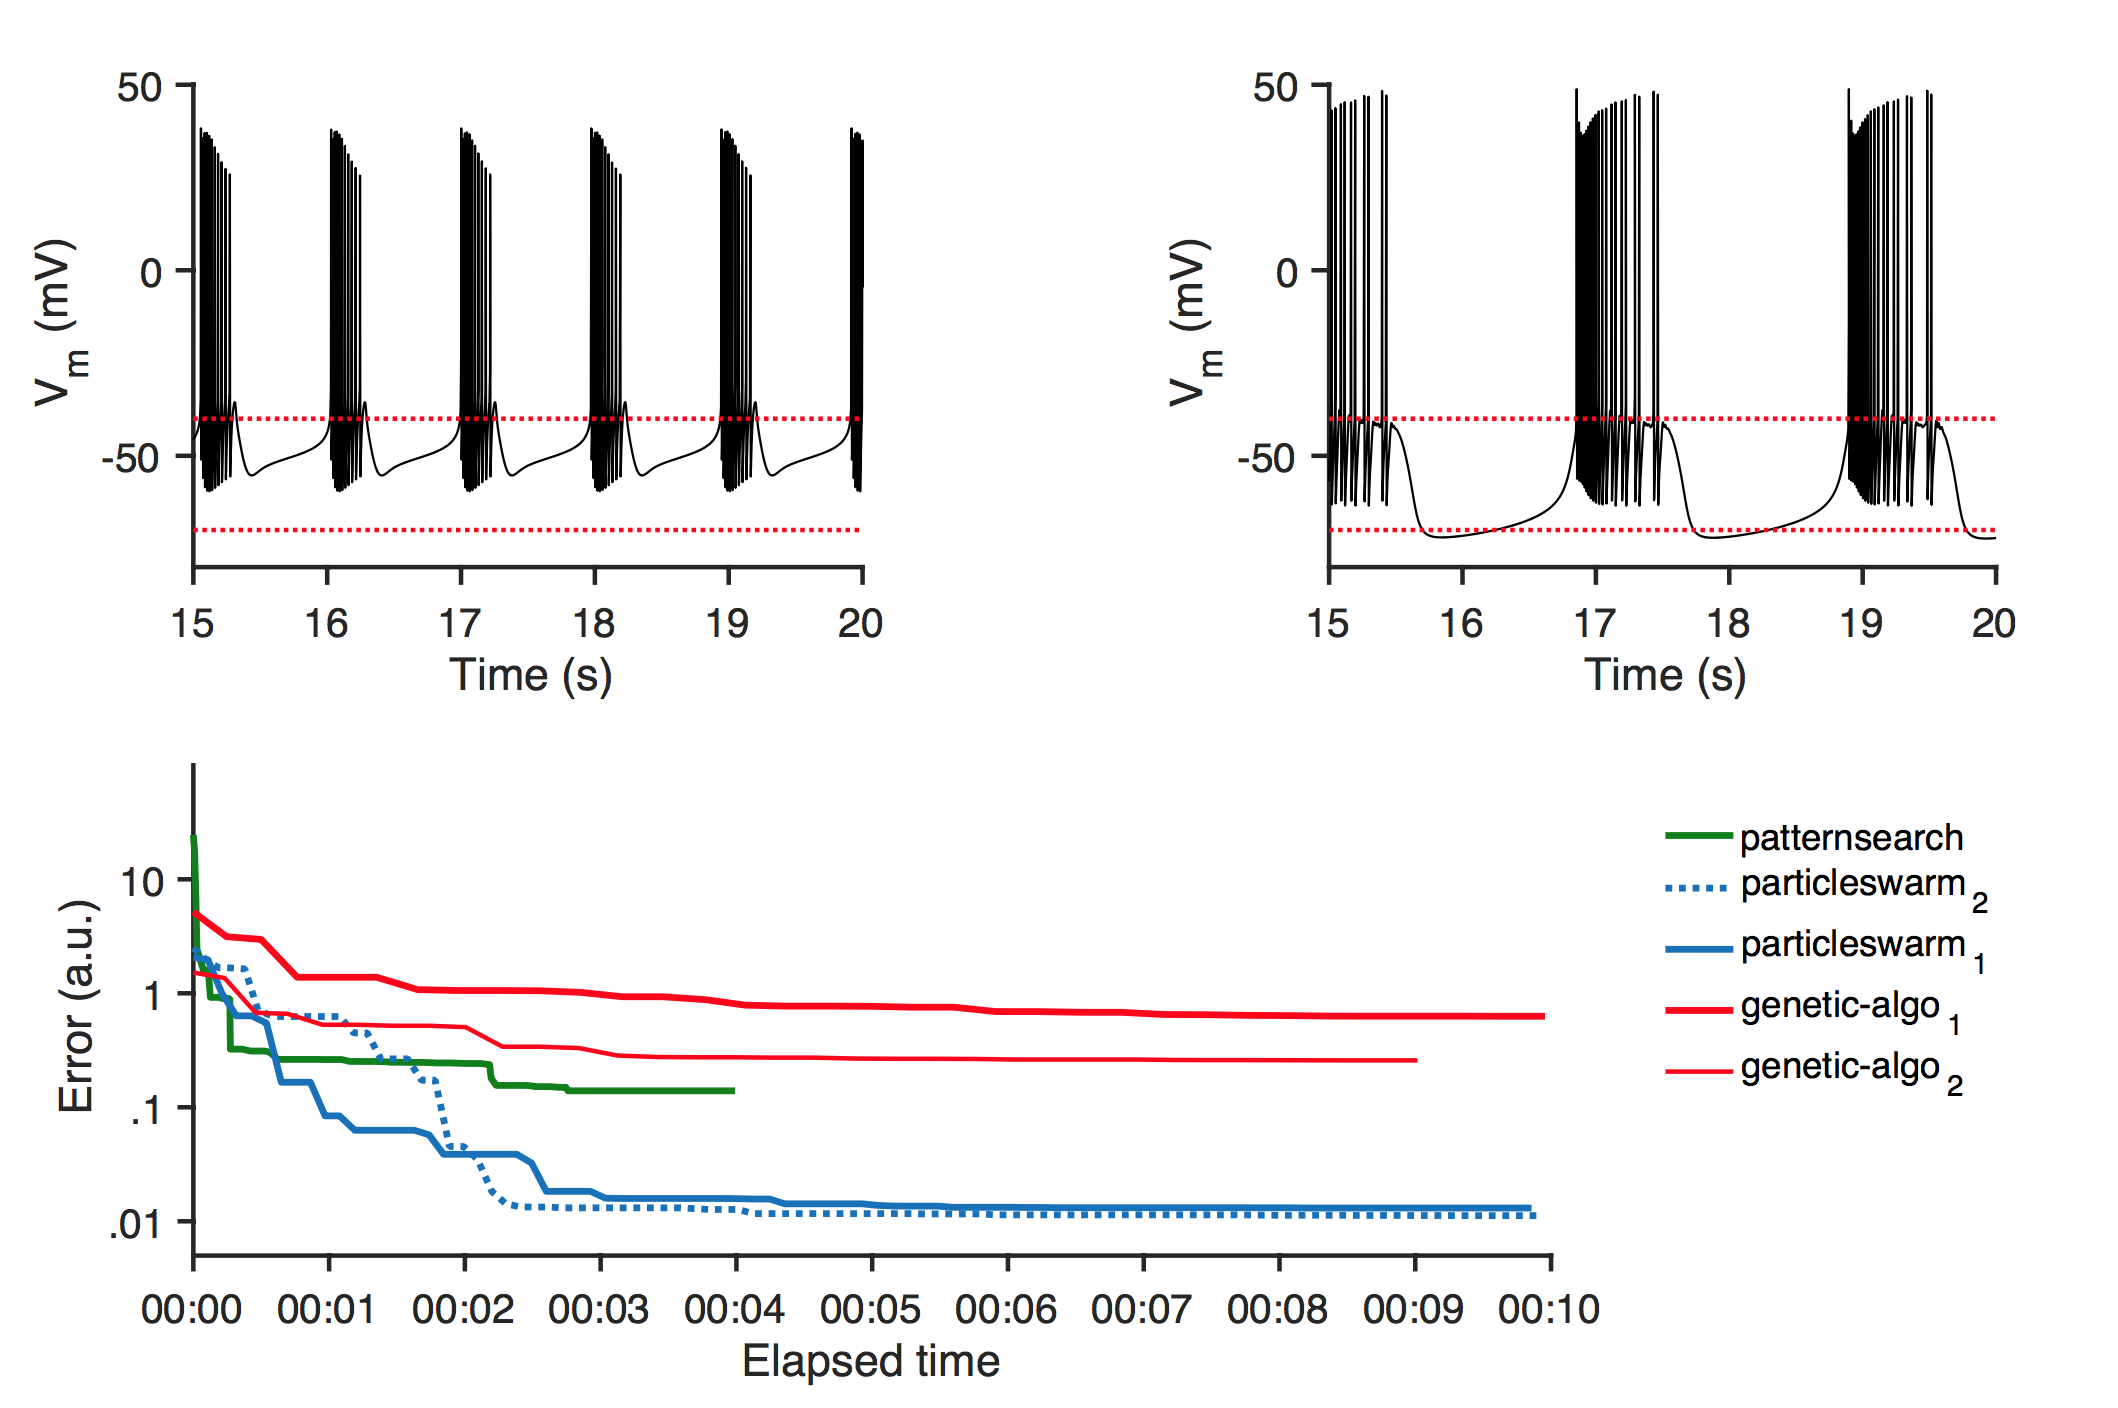
\includegraphics[width=1.0\linewidth]{gfx/ProcrustesExample}
	\caption[Parameter optimization using different algorithms]{Particle swarm optimization finds high-dimensional neuronal models with arbitrary constraints faster than other common algorithms. The top left trace displays a single-compartment seed. The top right trace displays the solution after optimization. Metrics for optimization were burst-frequency of 0.5 Hz, duty cycle of 0.3, and a slow wave bounded by $[-70, -40]$ mV where the spike troughs are above the slow wave. The bottom trace shows three optimization algorithms beginning with the same seed. Optimization terminates after 10 min or at a local minimum, as set by optimizer options. Figure by S. Gorur-Shandilya.}
	\label{fig:procrustesexample}
\end{figure}

\FloatBarrier

\subsection{Computing Metrics} \label{sec:metrics}
Simulation of a conductance-based model elicits voltage and calcium traces. The peaks of the calcium trace indicate the points of greatest spike density in the voltage traces. For a stationary signal, the burst period is the mean time between calcium peaks. The duty cycle is the ratio between burst duration and burst period. The time between the end of a burst of one cell and the beginning of a burst in another cell is the gap. Similarly, the delay is the time from a start of one burst in one cell to the beginning of a burst in another.

\begin{align}
	\mathrm{burst~period} &= mean(\mathrm{calcium~peaks}) = \frac{1}{\mathrm{burst~frequency}} \\
	\mathrm{duty~cycle} &= \frac{\mathrm{burst~duration}}{\mathrm{burst~period}}
\end{align}

\begin{figure}[h]
	\centering
	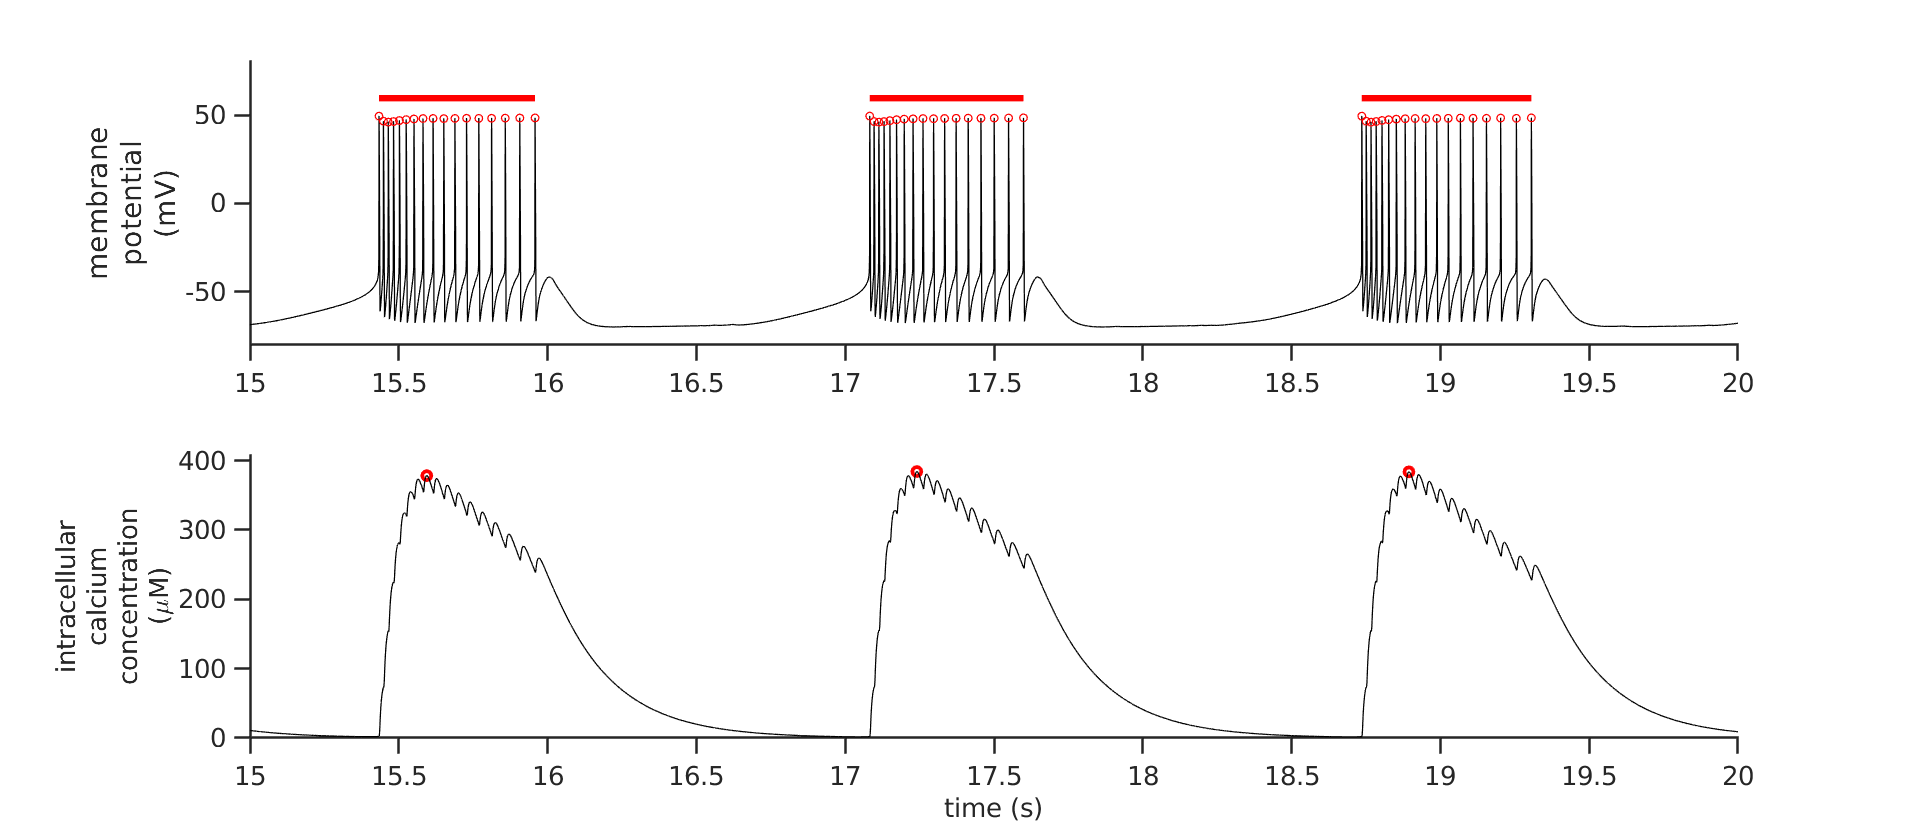
\includegraphics[width=1.0\linewidth]{gfx/BurstMetrics}
	\caption[Estimating burst metrics]{Estimating burst metrics. On the top trace, red dots show spike peak locations. The red bar indicates the burst duration. The bottom trace displays red dots at the calcium peaks.}
	\label{fig:burstmetrics}
\end{figure}

\subsection{Designing the Cost Function} \label{sec:cost}
For evaluations of three-compartment network models, the cost function computes the cost, burst frequency, duty cycle, mean spikes per burst, and the global minimum and maximum of the slow wave at several values of modulatory input into one or more cells. 

First the function evaluates whether the model elicits network activity within normal limits for real pyloric circuits. Once this has been confirmed at all steps of modulatory input current, the model targets ratios in various metrics to fine-tune solutions towards target activity.

\subsubsection{Evaluate Models for Pyloric Activity}
The first step confirms that the model is triphasic and pyloric. Burst periods, mean spikes per burst, burst durations, duty cycles, inter-burst periods, and delay between the starts of each burst were computed. If within an acceptable range, the cost was set to zero and penalized by by a normalized cost if outside the range. This range is set by experimental results. Normal pyloric networks fall within the following bounds.

\begin{table}[h]
	\myfloatalign
	\begin{tabularx}{\textwidth}{lll} \toprule
		\tableheadline{Metric} & \tableheadline{Lower} & \tableheadline{Upper} \\ \midrule
		calcium peak coefficient of variation & 0 & 0.1 \\
		burst period (s) & 0.3 & 2 \\
		spikes per burst & 4 & 30 \\
		burst duration (s) & 0.2860 & 1.4 \\
		duty cycle & 0.2050 & 0.4250 \\
		inter-burst period from \acs{AB}-\acs{PD} to \acs{LP} (s) & 0.112 & 0.33 \\
		inter-burst period from \acs{LP} to \acs{PY} (s) & -0.121 & -0.001 \\
		delay from \acs{AB}-\acs{PD} to \acs{LP} (s) & 0.6340 & 0.9720 \\
		delay from \acs{AB}-\acs{PD} to \acs{PY} (s) & 0.9250 & 1.3570 \\
		\bottomrule
	\end{tabularx}
	\caption[Pyloric network metric bounds]{Pyloric network metric bounds.}  
	\label{tab:metricsbounds}
\end{table}

For a value $v$ and target bounds $b_{low}$, $b_{high}$, the computed cost is

\begin{equation}
	\mathrm{cost} \propto 1 - \Bigg| \frac{b_{high} - b_{low}}{b_{high} + b_{low} + 2v} \Bigg|
\end{equation}

outside the bounds and zero within bounds. The first 50\% (10 s) of simulation were discarded as transient and spike times were computed by positive crossings of the zero line. If the network is bursting with an appropriate number of spikes, the model is checked for depolarization block, in which the membrane is depolarized but cannot spike. The voltage between each spike is recorded and each inter-spike interval within the burst is checked against the mean inter-spike interval for the burst to confirm that the compartment is regularly spiking during the burst. If any of these tests fail, the cost function returns a high cost and the exits the simulation.

There are several advantages to this preliminary step. First, the high cost guarantees that the failing candidate solution will not be the lowest-cost solution in the swarm, meaning that other models will not repeat the same optimization steps. Second, exiting the simulation saves time, since this solution will be discarded in any case.

As initial parameters for parameter optimization over response to modulatory input, 1,148 network models with a cost of zero in the decentralized condition were used. This dataset is available upon request.

\subsubsection{Response to Modulatory Input}
If candidate solutions pass pyloricity tests in the modulated and decentralized cases, the solution is further refined. The burst frequency, duty cycle, mean number of spikes per burst, and minimum and maximum of the slow wave are computed. A Savitzky-Golay filter with a window size of 300 ms is used to determine the maximum of the slow wave. In all other cases, the raw trace is used.

\begin{figure}[h]
	\centering
	\includegraphics[width=1.0\linewidth]{gfx/SavitzkyGolay}
	\caption[Savitzky-Golay filter visualizes slow wave]{Estimating slow wave maxima using a first-order Savitzky-Golay filter with a window of 300 ms applied to the voltage trace of a bursting neuron. A Savitzky-Golay filter is a convolutional digital filter which fits sub-sets of adjacent data to a low-degree polynomial by the least squares method. This has the effect of smoothing high-amplitude, high-frequency oscillations, without strongly distorting low-frequency signal components\autocite{SavitzkySmoothingDifferentiationData1964}.}
	\label{fig:savitzkygolay}
\end{figure}


The ratio between metrics in the modulated and decentralized case are computed. Targeting a ratio has several benefits. First, it is agnostic to initial neuron parameters. For instance, burst frequencies in healthy pyloric circuits commonly vary on the interval $[0.5, 1.5]$ Hz between preparations\autocite{MarderUnderstandingCircuitDynamics2007}. By computing a ratio, the response is normalize to the basal activity of the model, preventing over-fitting. In addition, examining two values of maximal conductance, rather than a series of linearly-spaced values significantly cuts down on computational complexity. While only two points were specified in the ratio, the constraint of pyloricity means the cost function strongly favors models with graded increase with respect to increasing modulatory input. For single-neuron simulations, this constraint does not exist.

Because the change in slow wave amplitude is a signed quantity, the slow wave maximum towards a +5 mV increase instead of a rational change.

\begin{table}
	\myfloatalign
	\begin{tabularx}{\textwidth}{lll} \toprule
		\tableheadline{Metric} & \tableheadline{Ratio} & \tableheadline{Change} \\ \midrule
		burst frequency & 1.5 & \\
		duty cycle & 1.0 & \\
		slow wave maximum & & +5 mV \\
		slow wave minimum & & -5 mV \\
		\bottomrule
	\end{tabularx}
	\caption[Pyloric network metric ratios]{Pyloric network metric target ratios and changes between the modulated and decentralized cases.}  
	\label{tab:metricsratios}
\end{table}

Graded increases, where the cost is summed for each point along the \acs{IMI} maximal conductance range, was only used for single-neuron fitting of models to dose-response data. In this regime, metric values are specified for each value of modulatory input maximal conductance. This method has the advantage of increasing the cost on models which do not exhibit graded responses to modulatory input, but is computationally expensive and may result in over-fitting.



%*****************************************
%*****************************************
%*****************************************
%*****************************************
%*****************************************

%\addtocontents{toc}{\protect\clearpage} % <--- just debug stuff, ignore
%************************************************
\chapter{Results}\label{ch:results} % $\mathbb{ZNR}$
%************************************************
Decentralized \acs{STG} preparations have descending modulatory inputs from the \acsp{CoG} and \acs{OG} removed. \acs{STG} neurons in a decentralized state exhibit a slower burst frequency and variable network activity\autocite{HamoodAnimaltoanimalvariabilityneuromodulation2014, HamoodConsequencesacutelongterm2015}. This effect can be restored to normal function by exogenous application of modulatory substances into the saline bath\autocite{SwensenModulatorsconvergentcellular2001, SharpDynamicclampcomputergenerated1993}. Proctolin and \acs{RPCH} are neuromodulators which open a mixed cation inward modulatory input current \ac{IMI}\autocite{SwensenModulatorsconvergentcellular2001}. 

To model decentralization and modulation, single-neuron \ac{AB} models and network (\acs{AB}-\acs{PD}, \acs{LP}, \acs{PY}) models were constructed according to the Hodgkin-Huxley formalism\autocite{PrinzAlternativehandtuningconductancebased2003, PrinzSimilarnetworkactivity2004, HodgkinMeasurementcurrentvoltagerelations1952, Hodgkincomponentsmembraneconductance1952, Hodgkinquantitativedescriptionmembrane1952}. Maximal conductances were determined by particle swarm optimization (\autoref{sec:parameteroptimization}) to respond to modulatory input in the form of \acs{IMI}\autocite{SwensenModulatorsconvergentcellular2001}. \acs{AB} and the two \acs{PD} cells were combined into a computational composite \acs{AB}-\acs{PD} since the cells are strongly electrically coupled (\autoref{fig:prinz1}). Similarly, electrically-coupled \acs{PY} cells were combined into a single computational composite, following \citeauthor{PrinzSimilarnetworkactivity2004}\autocite{PrinzSimilarnetworkactivity2004} The \acs{AB}-\acs{PD} pacemaker kernel synapses onto \acs{LP} and \acs{PY} with inhibitory glutamatergic and cholinergic synapses. \acs{LP} and \acs{PY} reciprocally inhibit each other and \acs{LP} feeds back onto the pacemaker kernel (\autoref{fig:pyloricrhythm}).

\acs{AB} increases in frequency and amplitude from baseline in bath-applied proctolin\autocite{SharpDynamicclampcomputergenerated1993, SwensenMultiplepeptidesconverge2000, SwensenModulatorsconvergentcellular2001, GolowaschProctolinactivatesinward1992}. Modulatory input conductance (\autoref{sec:modulatoryinput}) was added to single-compartment models from the Prinz database\autocite{PrinzAlternativehandtuningconductancebased2003} to characterize the effect of \acs{IMI} on a population of previously studied models. Most models did not respond to \acs{IMI}, so maximal conductances were manipulated in a particle swarm optimization protocol to produce models which increase in frequency and amplitude to increasing \acs{IMI} maximal conductance\autocite{NusbaumNeuronalRoleCrustacean1988,SharpDynamicclampcomputergenerated1993}.

\acs{RPCH} activates a modulatory input conductance in \acs{AB} and \acs{LP} cells. Network models were simulated under \acs{IMI} conductance in \acs{AB}-\acs{PD}, \acs{LP} and both model neurons to simulate neuromodulation by \acs{RPCH}. Maximal conductances of the three model neurons and synapses were manipulated by particle swarm optimization to produce models with slow, unstable rhythms in the decentralized condition and increased burst frequency and amplitude under neuromodulation. While modulation onto the pacemaker and \acs{LP} recapitulated experimental findings (\autoref{fig:rosenbaum2}), modulation into \acs{AB}-\acs{PD} and \acs{LP} produced the most stable rhythms. 

\section{Modulation in AB Models Switches Between Amplitude States}
To develop an initial set of solutions to optimize (the ``seed''), neurons from the \acs{STG} neuron database were simulated\autocite{PrinzAlternativehandtuningconductancebased2003}. This database contains ~2.2 million model neurons with linearly spaced parameters. Neurons flagged as ``bursting neurons'' were simulated with increasing levels of modulatory input. Since \acs{AB} does not fire strong action potentials (\autoref{fig:sharp2}) and responds to \acs{RPCH} under the potent sodium channel blocker \acs{TTX}, \ac{INa} and \acs{ICaT} maximal conductances set to zero to eliminate sodium and calcium spikes respectively\autocite{NusbaumNeuronalRoleCrustacean1988}. These models would serve as a testbed for exploring neuromodulation in isolated cells.

Quiescent models were defined as having amplitude < 20 mV to isolate models that appear similar to decentralized preparations in \ac{TTX}\autocite{NusbaumNeuronalRoleCrustacean1988}. Slow wave amplitude was defined as the maximal peak voltage minus the minimal trough voltage at steady-state ($10~\mathrm{s} < t < 20~\mathrm{s}$).

Modulatory input was applied to these low-amplitude oscillators ($n = 14,700$), which were simulated for 20 s (\autoref{fig:prinzburstingmodelsnavcatswensen}). The first 10 s were discarded as transient and burst frequency and amplitude were computed. To test sensitivity to initial conditions, the simulations were repeated with $V_m = 60$ mV and $m_{MI} = 1$ instead of standard initial conditions (\autoref{tab:initialconditions}). No significant differences were observed.

\begin{figure}[h]
	\centering
	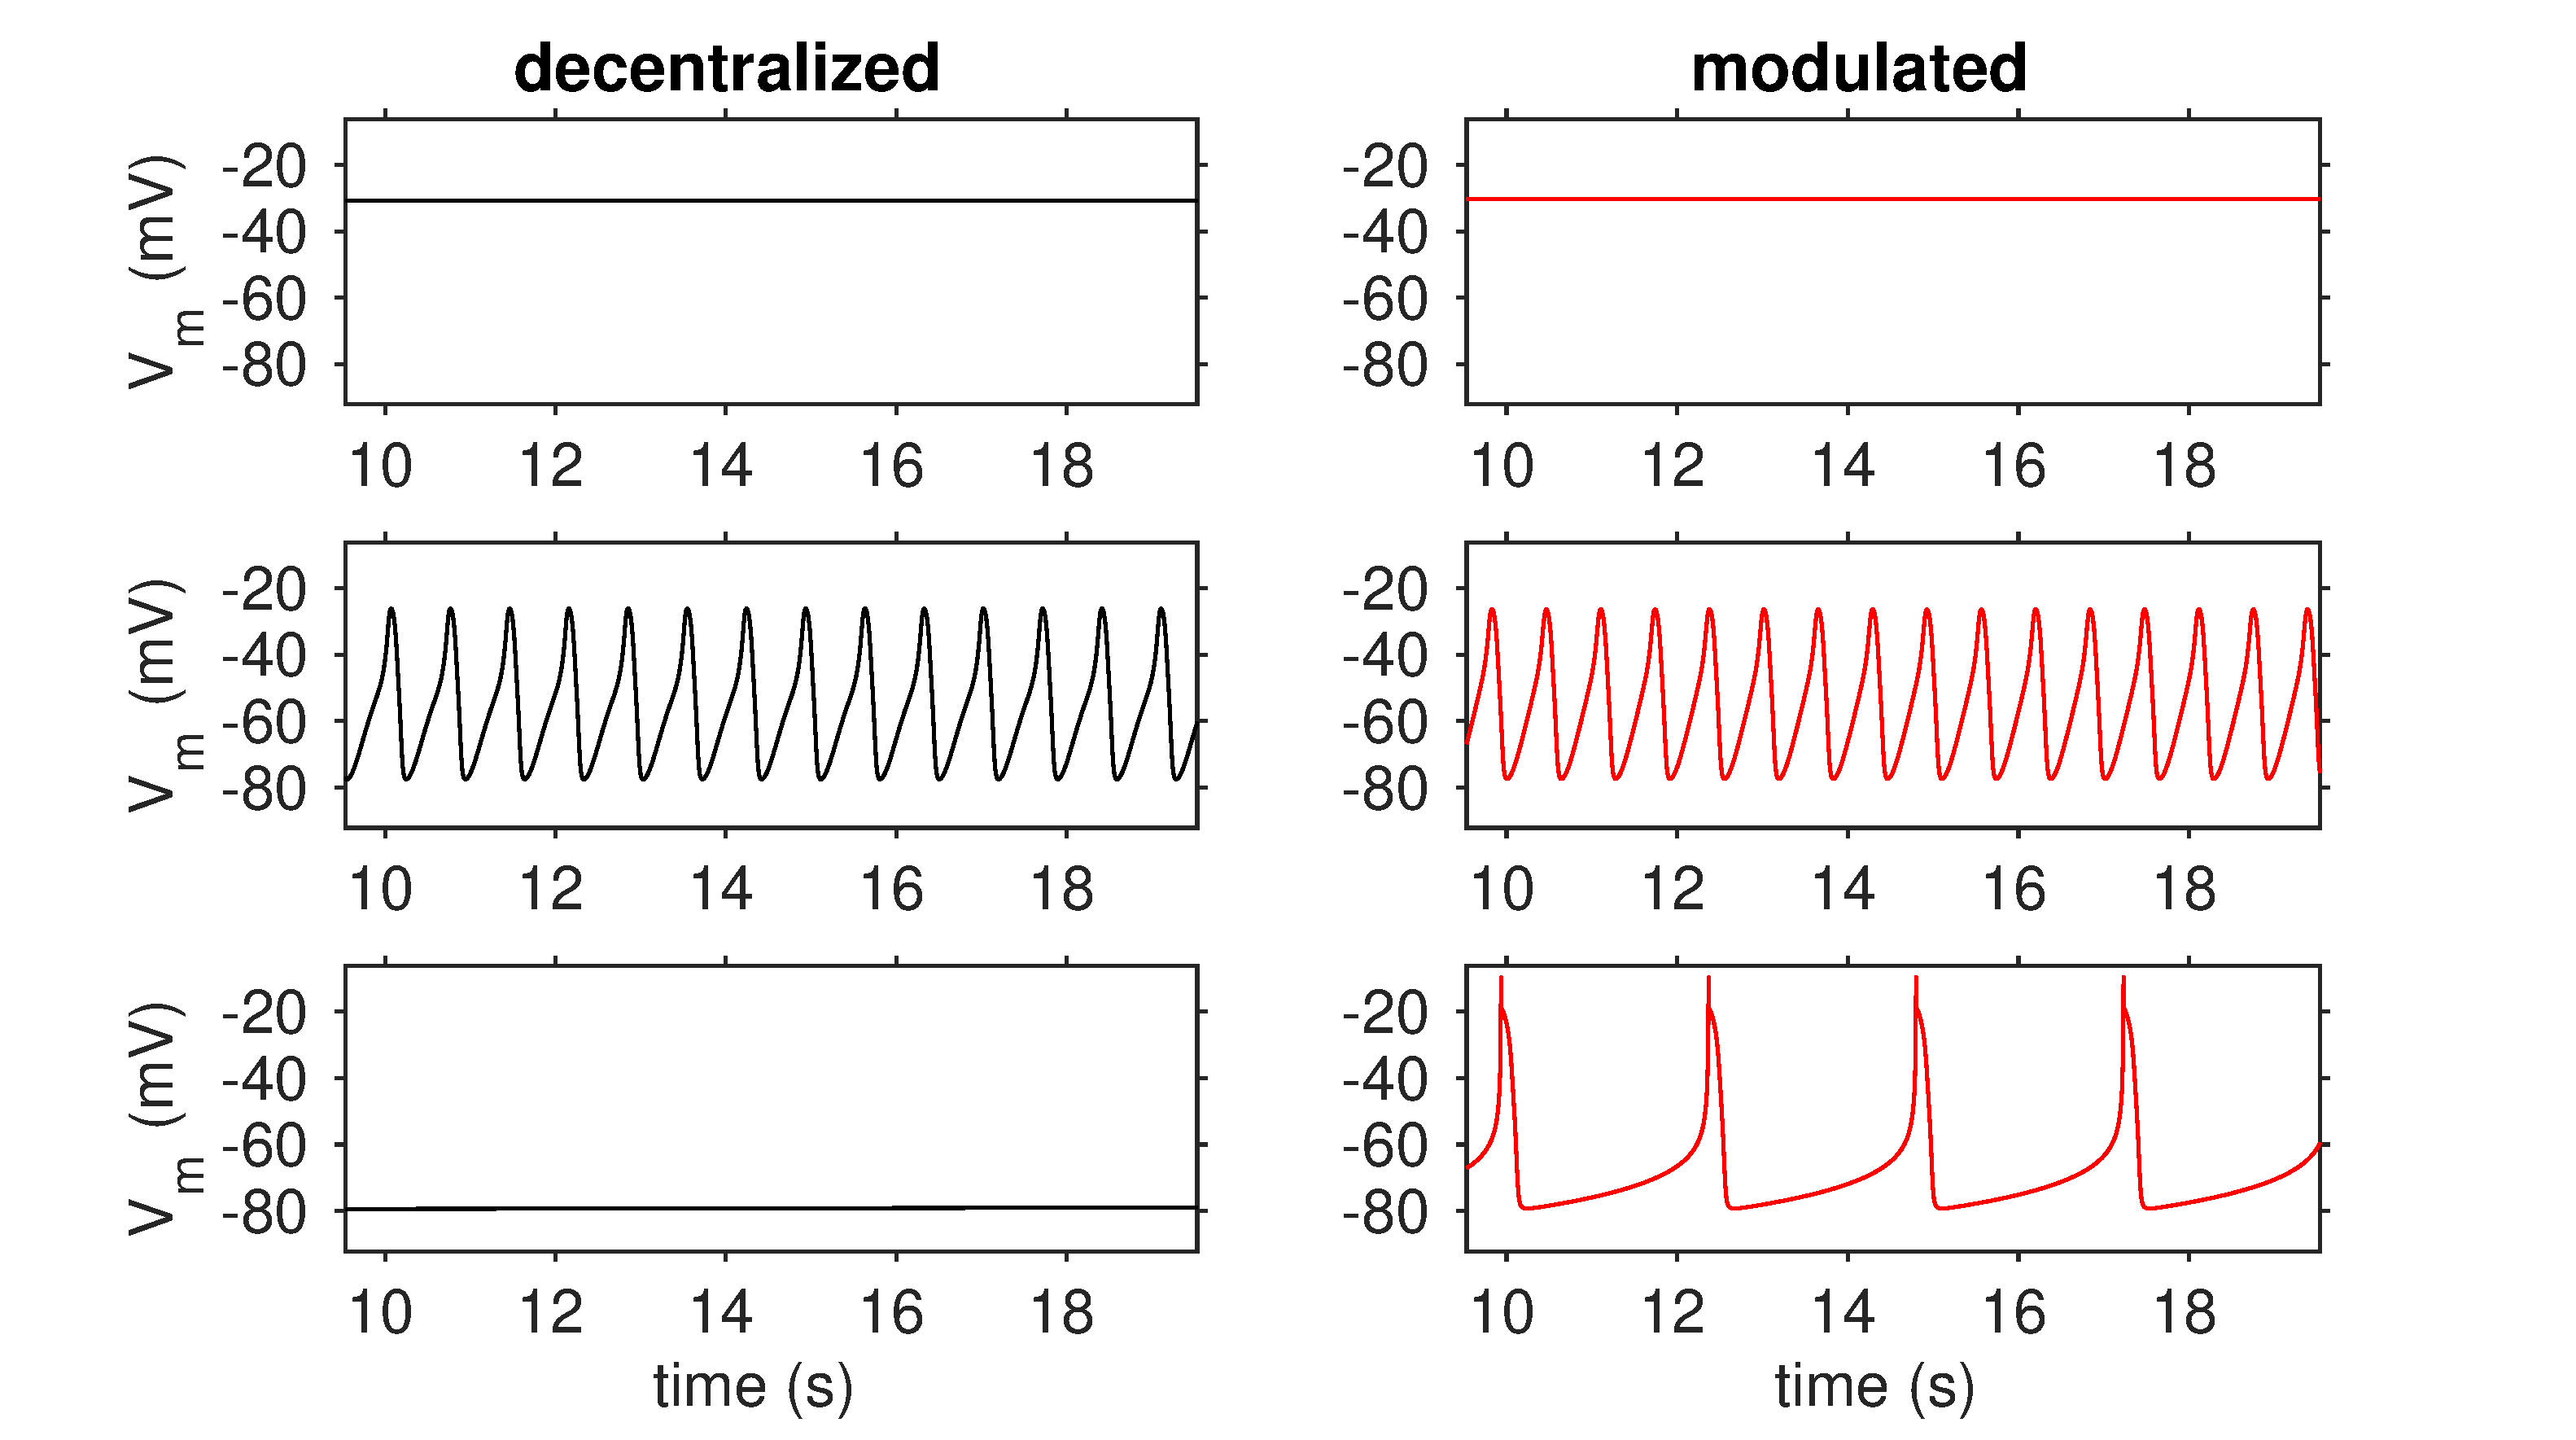
\includegraphics[width=1.0\linewidth]{gfx/prinz-models/tracePrinz}
	\caption[Three motifs of modulation in model AB neurons]{Three motifs of modulation in model \acs{AB} neurons from the \acs{STG} database.  Most model neurons from the Prinz \acs{STG} database without \acs{INa} or \acs{ICaT} conductance remained quiescent. A subset of models oscillated in both conditions and < 100 switched from quiescence to oscillation. Black traces demonstrate the non-modulated case and red traces indicate $\bar{g}_MI = 1~\mu \mathrm{S/mm^2}$.}
	\label{fig:traceprinz}
\end{figure}

\begin{figure}[h]
	\centering
	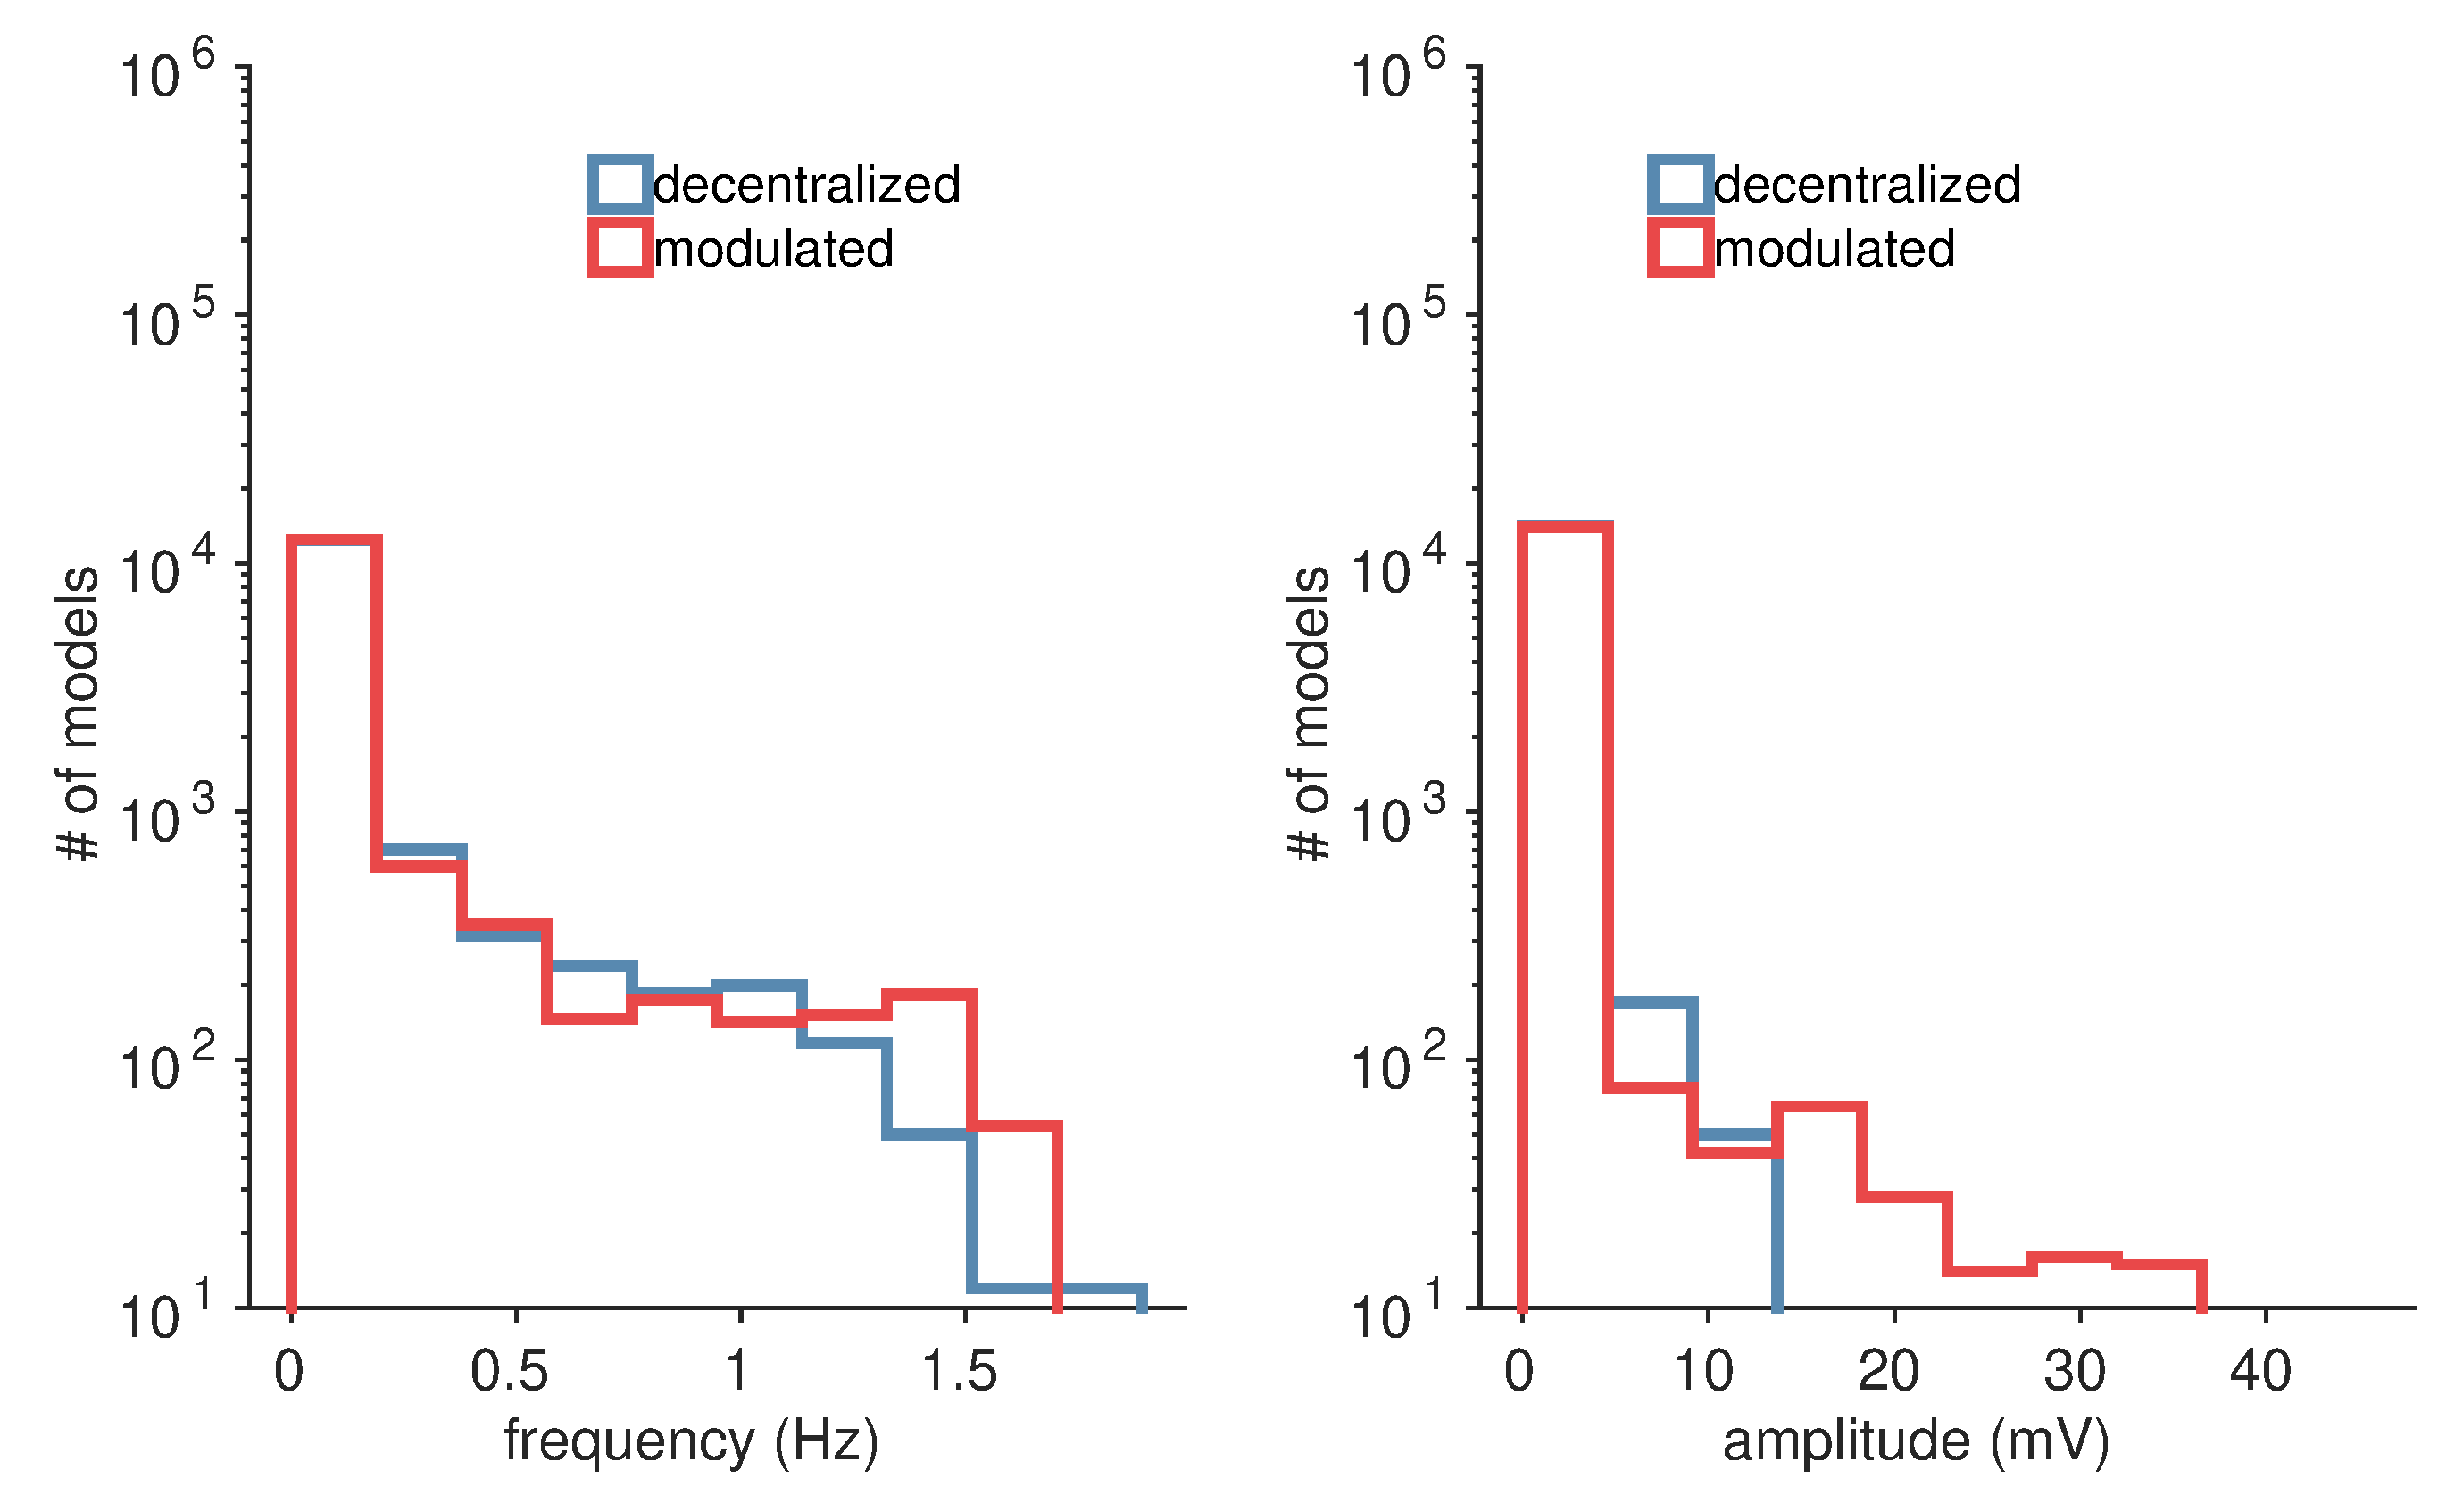
\includegraphics[width=1.0\linewidth]{gfx/prinz-models/histPrinz}
	\caption[Summary statistics of database models with modulatory input]{Most database models without \acs{INa} or \acs{ICaT} do not respond to modulatory input.}
	\label{fig:histprinz}
\end{figure}

Only a small subset of the models exhibited changes burst frequency and amplitude (\autoref{fig:histprinz}). \autoref{fig:traceprinz} illustrates three motifs in order of rarity. Most commonly, models with and without modulatory input were quiescent. A subset of models exhibited subthreshold voltage oscillations in both decentralized and modulated cases. The 1000 models with the greatest change in frequency and amplitude were replotted (\autoref{fig:prinzburstingmodelsnavcatexcisedswensen}). Models exhibit a sharp increase in peak voltage over a small range of modulatory input. Frequency increases monotonically sudden jumps in magnitude.

The 100 models which responded to modulatory input in a graded manner with increasing frequency and amplitude were optimized using a gradient descent algorithm (\autoref{fig:figprinzburstingttxcatnoscgmiswensenexprosim3}). Since the modulatory input IV curve achieves maximal inward current at $V_m \approx -32$ mV, peak voltage at high values of \acs{IMI} maximal conductance tended to be at least this membrane potential. A subset of models achieved graded frequency increase, though amplitude showed a sharply peaked jump from small oscillations (< 10 mV) to amplitude indicative of biological \acs{AB} neurons (\autoref{fig:figprinzburstingttxcatnoscgmiswensenexprosim3}). These data suggest that a subset of models experience modulatory input current as a bistable switch between non-oscillatory and oscillatory states.

When models were optimized over a smaller range of \acs{IMI} maximal conductance ($\bar{g}_{MI} = [0, 0.2]~\mu\mathrm{S/mm^2}$), resultant solutions responded to modulatory input in a graded manner. The burst frequency and amplitude increase smoothly as functions of modulatory input, responding most strongly at low maximal conductance. We hypothesize several reasons for this effect. First, the total capacitance of a physiologically-realistic \acs{AB} neuron is much higher than in the model neurons used here\autocite{Soto-TrevinoComputationalmodelelectrically2005,TurrigianoSelectiveregulationcurrent1995}. Second, the elimination of several currents significantly reduced the input resistance so that \acs{IMI} contributes a greater proportion to the net instantaneous current. Thirdly, most solutions converged to small values of conductances. Since the membrane potential evolves proportionally to the instantaneous sum of the currents, relative proportions of conductance with respect to each other and the membrane capacitance determine the dynamics. A model neuron with small membrane capacitance and intrinsic conductances produces qualitatively different activity with smaller perturbations.

\begin{figure}
	\centering
	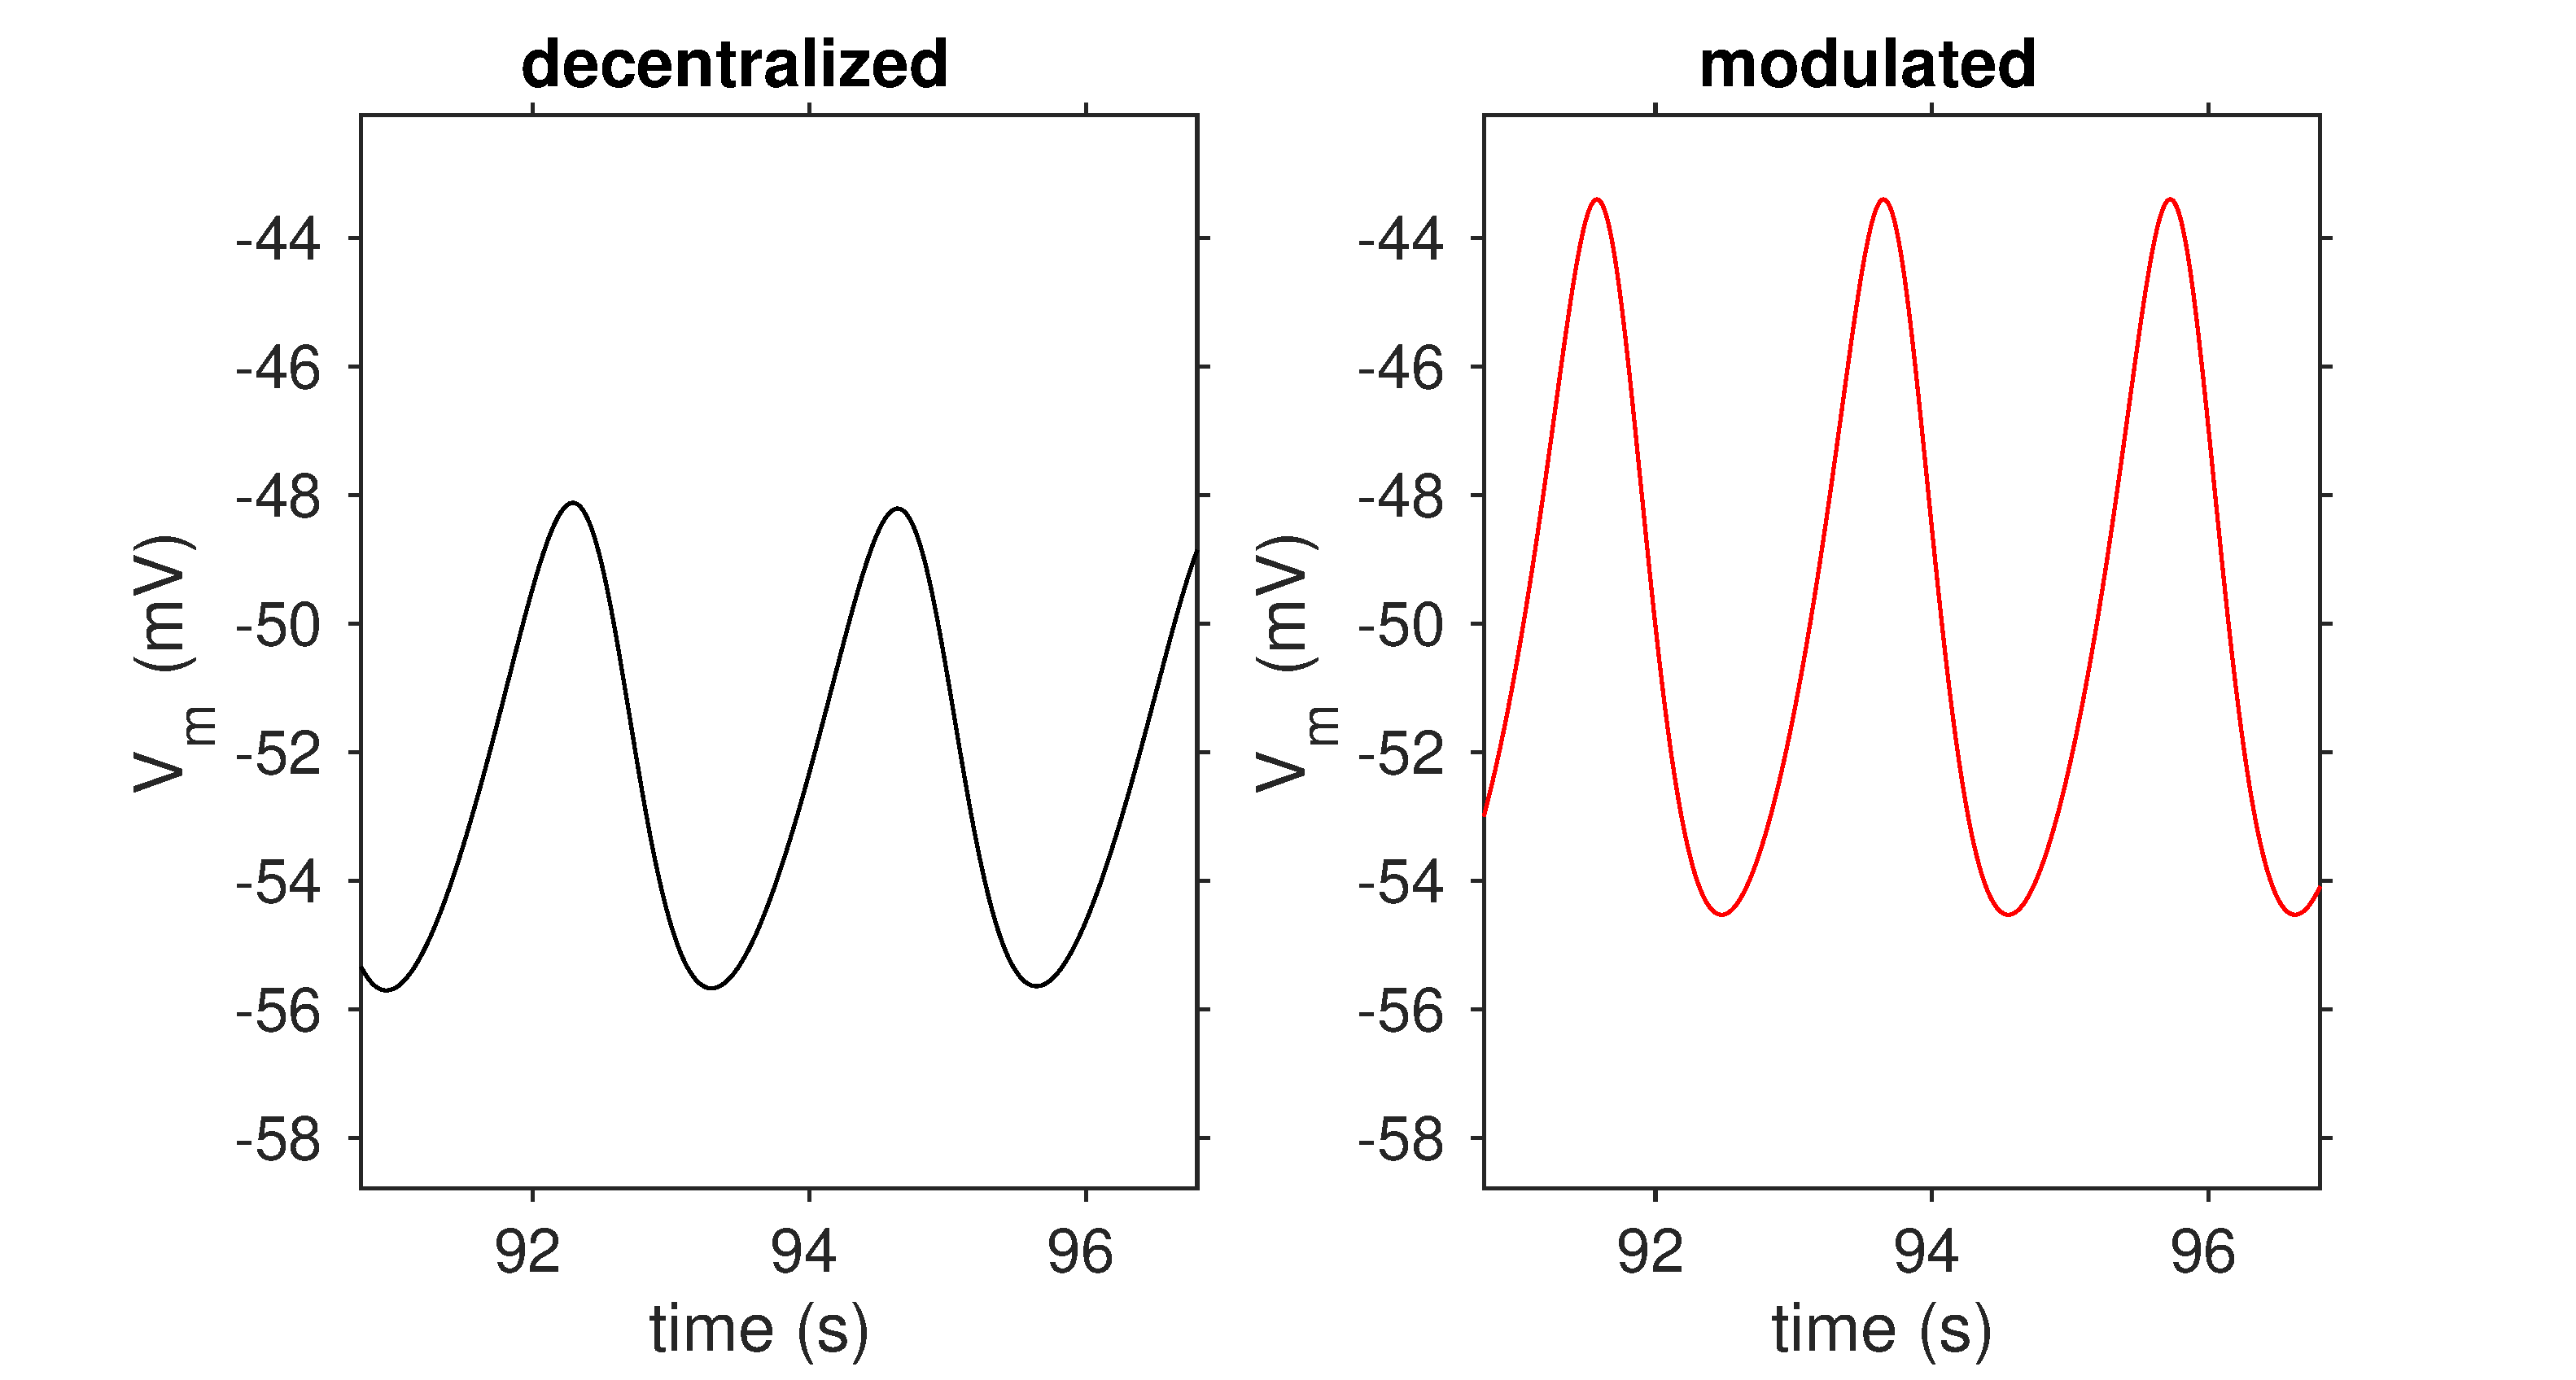
\includegraphics[width=1.0\linewidth]{gfx/prinz-models/ABwmod2}
	\caption[Superimposed model AB traces]{\acs{AB} model increases in amplitude and frequency with modulatory input. The model recapitulates electrophysiological recordings (\autoref{fig:sharp2}). Modulatory input current cannot replace slow calcium in its excitatory role, but a balance between \acs{IH}, \acs{ICaS}, and outward currents produce the conditions for \acs{IMI} to depolarize the membrane potential during voltage peaks.}
	\label{fig:abwmod}
\end{figure}

\FloatBarrier

\section{Variability in Network Response to Modulation}
\acs{RPCH} activates \ac{IMI} in the anterior burster (\acs{AB}) and lateral pyloric (\acs{LP}) cells of the \acs{STG}\autocite{NusbaumNeuronalRoleCrustacean1988}. To model the effects of \acs{RPCH} modulation in the pyloric circuit, \acs{IMI} was added to each cell and together in the network model (\autoref{fig:pyloriccircuit}) with \acs{AB} and \acsp{PD} reduced to a single composite pacemaker neuron (\acs{AB}-\acs{PD}). Particle swarm optimization (\autoref{sec:parameteroptimization}) selected for models which increased in burst frequency and slow wave amplitude over increasing modulatory input into \acs{AB}-\acs{PD}, \acs{LP}, and both model neurons. Maximal conductances for all ionic and synaptic currents were varied as parameters (28 parameters plus one for each cell with \acs{IMI}).

\subsection{Neuromodulation Increases Frequency and Amplitude}
Optimization produced models of the network with increased burst frequency and slow wave amplitude under modulation in the three conditions. Three motifs of network activity appeared several times in optimized solutions. Some model networks produced triphasic activity without modulation, and increased burst frequency and slow wave amplitude under neuromodulation. Others produced periodic, but not pyloric activity (e.g. skipped bursts) and rectified these errors under modulation. The third category contained quiescent and tonically-firing networks which become pyloric under modulation.

\autoref{fig:networkab47traces} displays an optimized network model with modulatory input into \acs{AB}-\acs{PD}. Without modulation, the network is stable, with a triphasic rhythm. Addition of modulatory input monotonically increases the burst frequency. The duty cycle for \acs{PY} decreases from 0.5 to 0.3. Similarly, the mean number of spikes per burst in \acs{PY} decreases. This indicates that the burst duration is decreasing and the mean inter-spike interval remains relatively constant. \acs{PY} is not able to increase in slow-wave amplitude until the duration and intensity of the bursts can be maintained at the higher frequency. 

\begin{figure}[h]
	\centering
	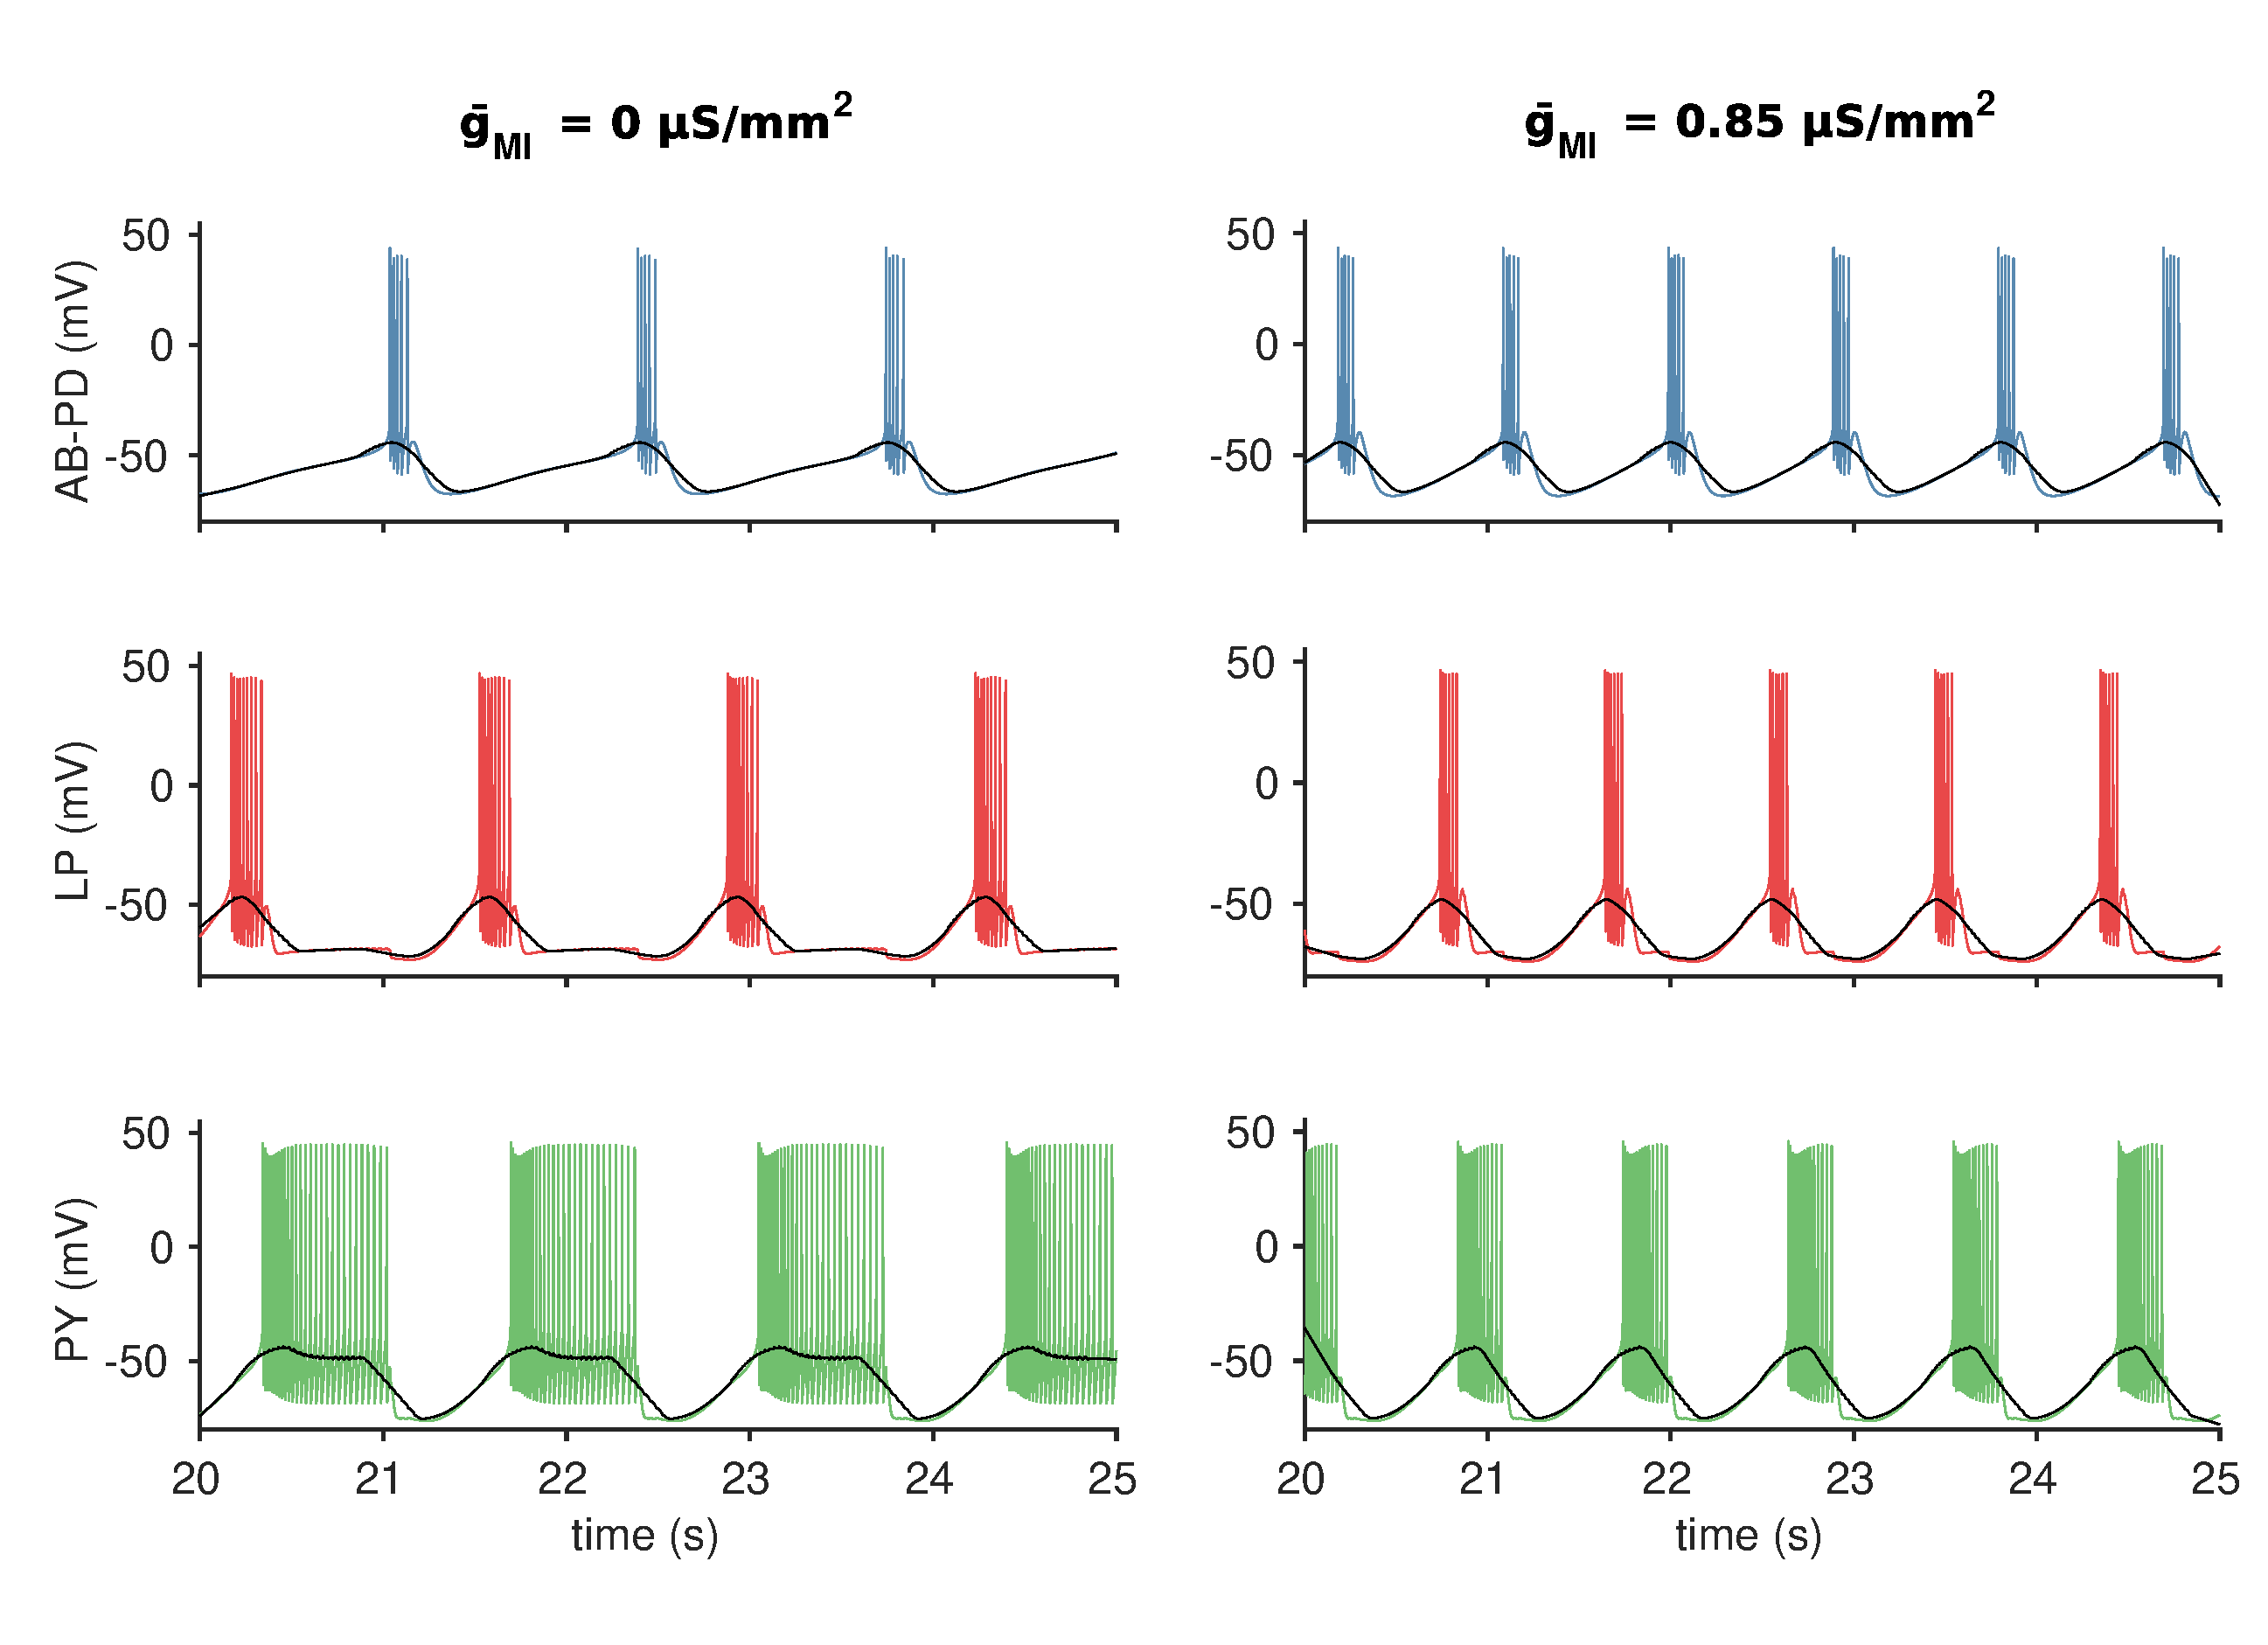
\includegraphics[width=1.0\linewidth]{gfx/network/network_AB_47_traces}
	\caption[Network with modulation into AB-PD (traces)]{Modulation into \acs{AB}-\acs{PD} increases burst frequency and \acs{AB}-\acs{PD} slow wave amplitude. Left-hand traces are without neuromodulation.. Right-hand traces have \acs{IMI} in \acs{AB}-\acs{PD} at $\bar{g}_{MI} = 0.85~\mu \mathrm{S/mm^2}$. Colors indicate cells (blue is \acs{AB}-\acs{PD}, red is \acs{LP}, green is \acs{PY} and overlaid black indicates the slow wave).}
	\label{fig:networkab47traces}
\end{figure}

\begin{figure}[h]
	\centering
	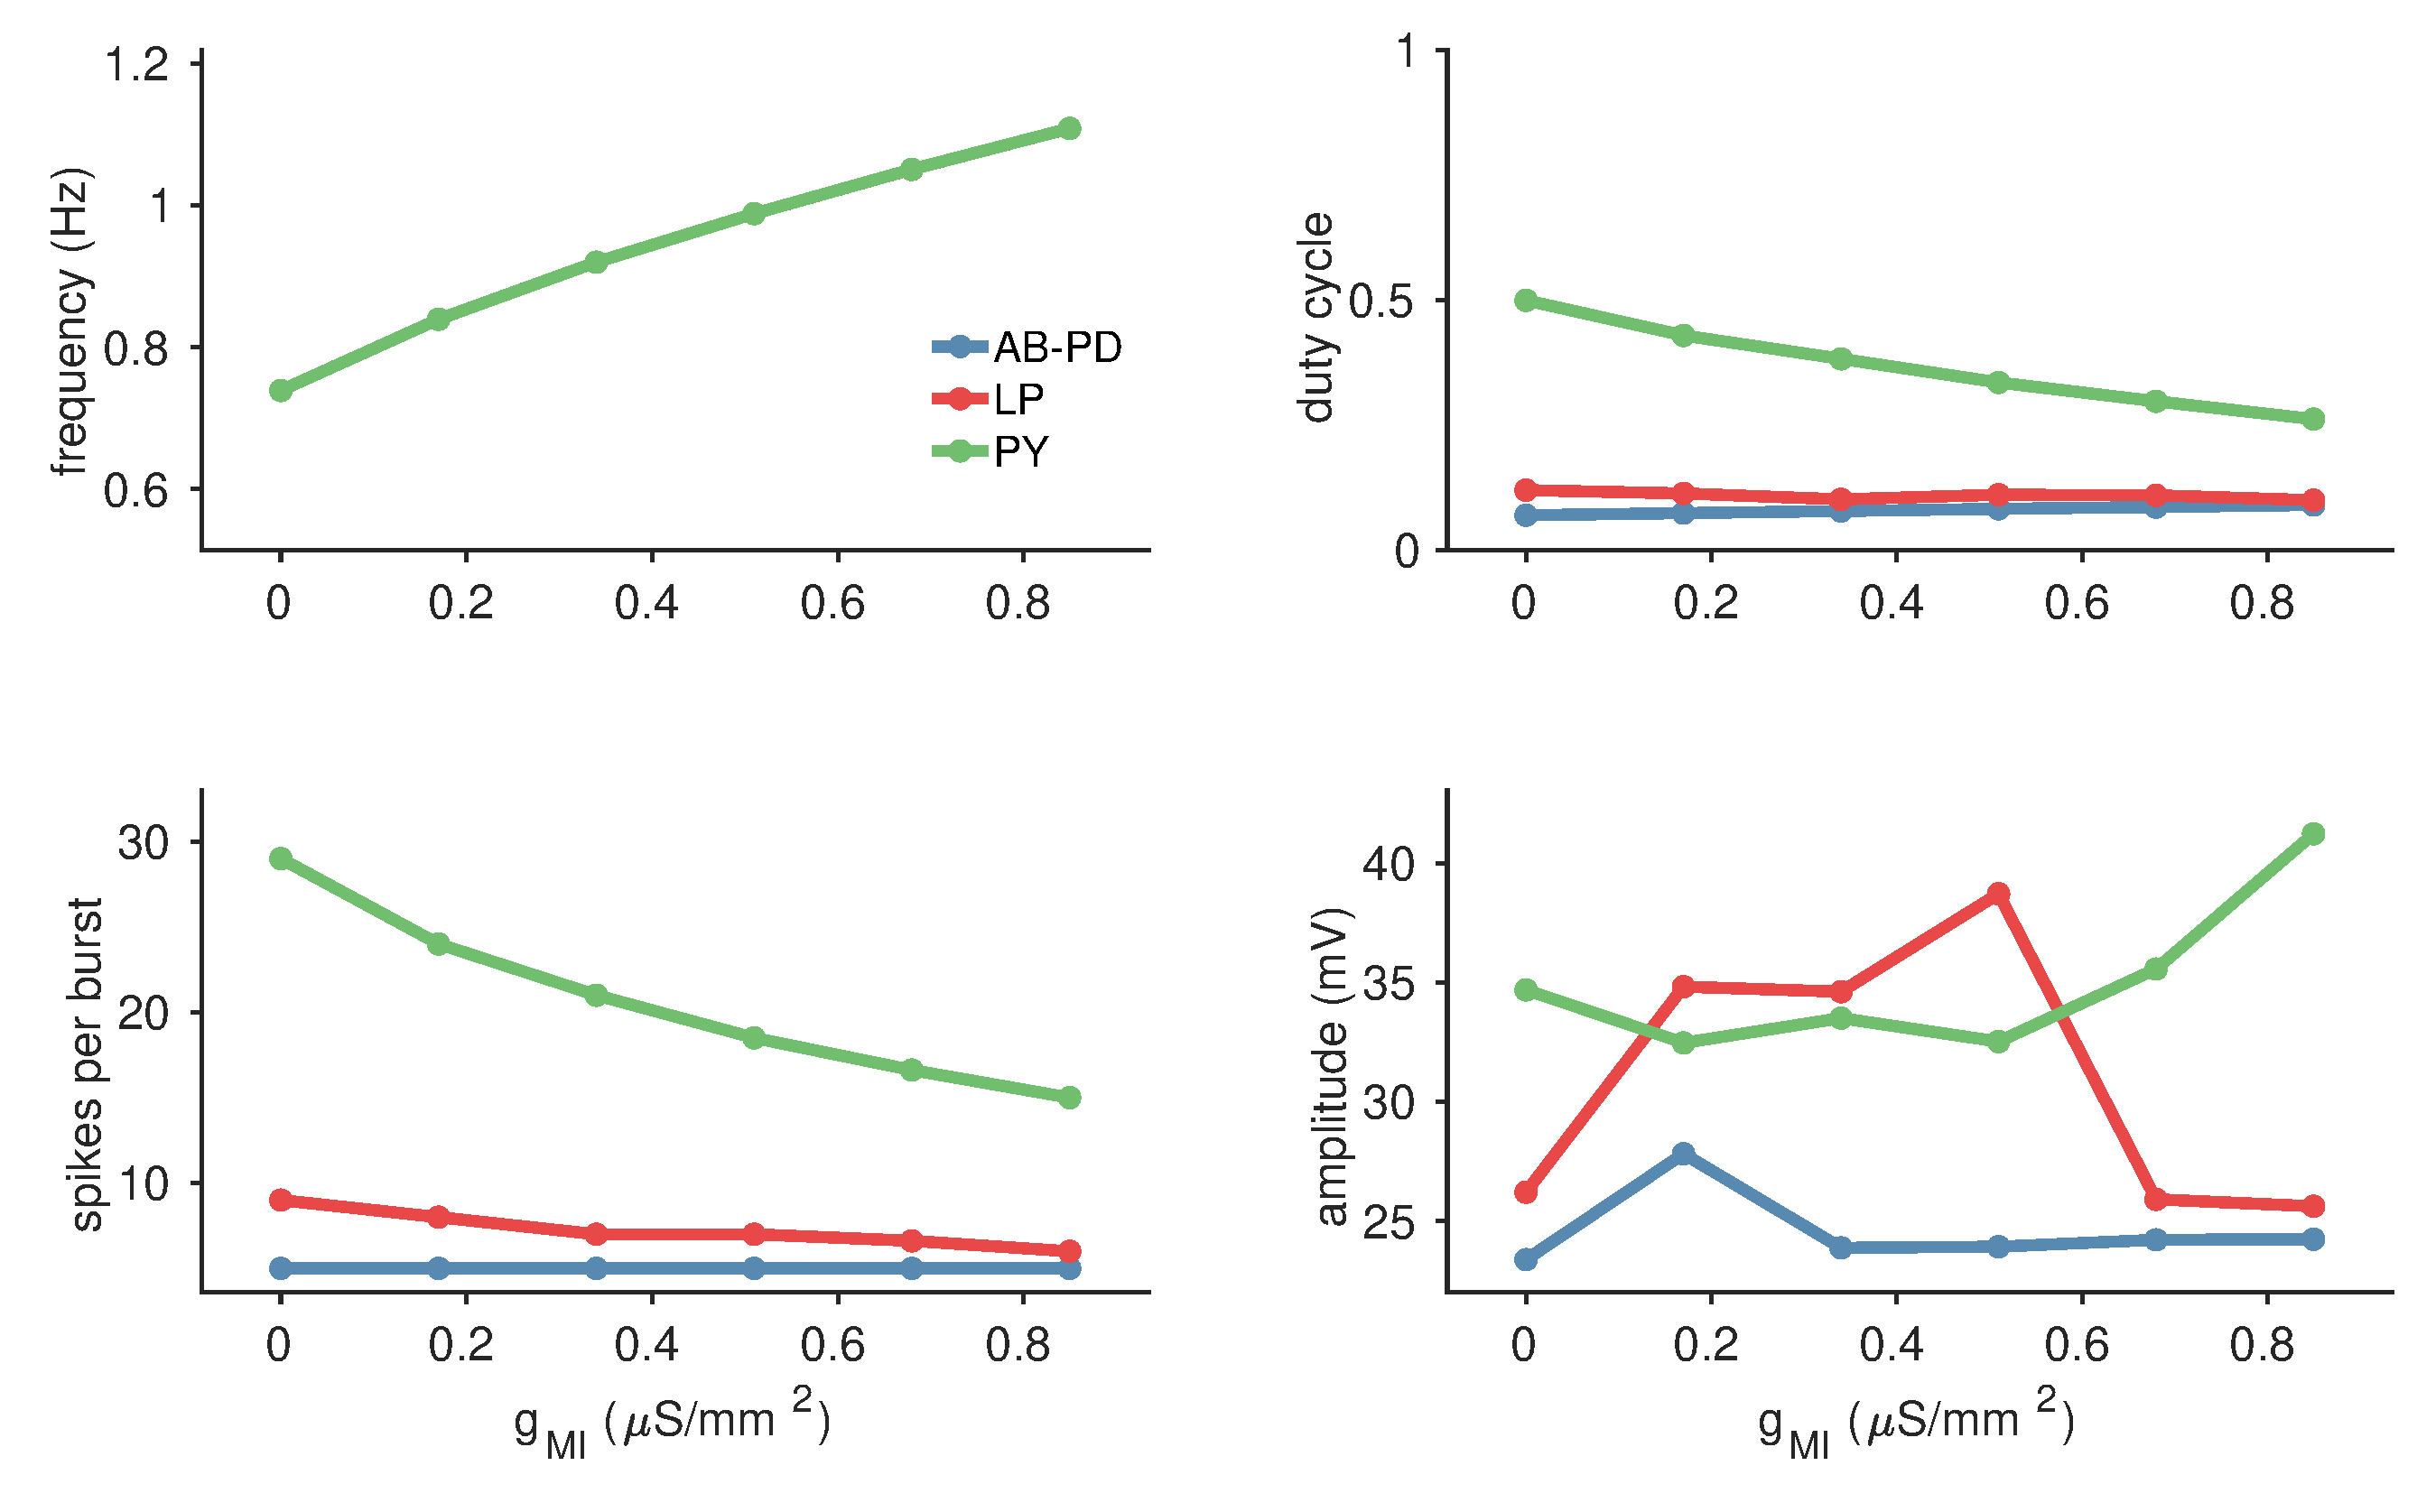
\includegraphics[width=1.0\linewidth]{gfx/network/network_AB_47_metrics}
	\caption[Network with modulation into AB-PD (metrics)]{Modulation into \acs{AB}-\acs{PD} increases burst frequency and \acs{AB}-\acs{PD} slow wave amplitude. Metrics at steady-state as a function of increasing modulatory input. Colors indicate cells (blue is \acs{AB}-\acs{PD}, red is \acs{LP}, green is \acs{PY}.}
	\label{fig:networkab47metrics}
\end{figure}

\FloatBarrier

\begin{figure}[h]
	\centering
	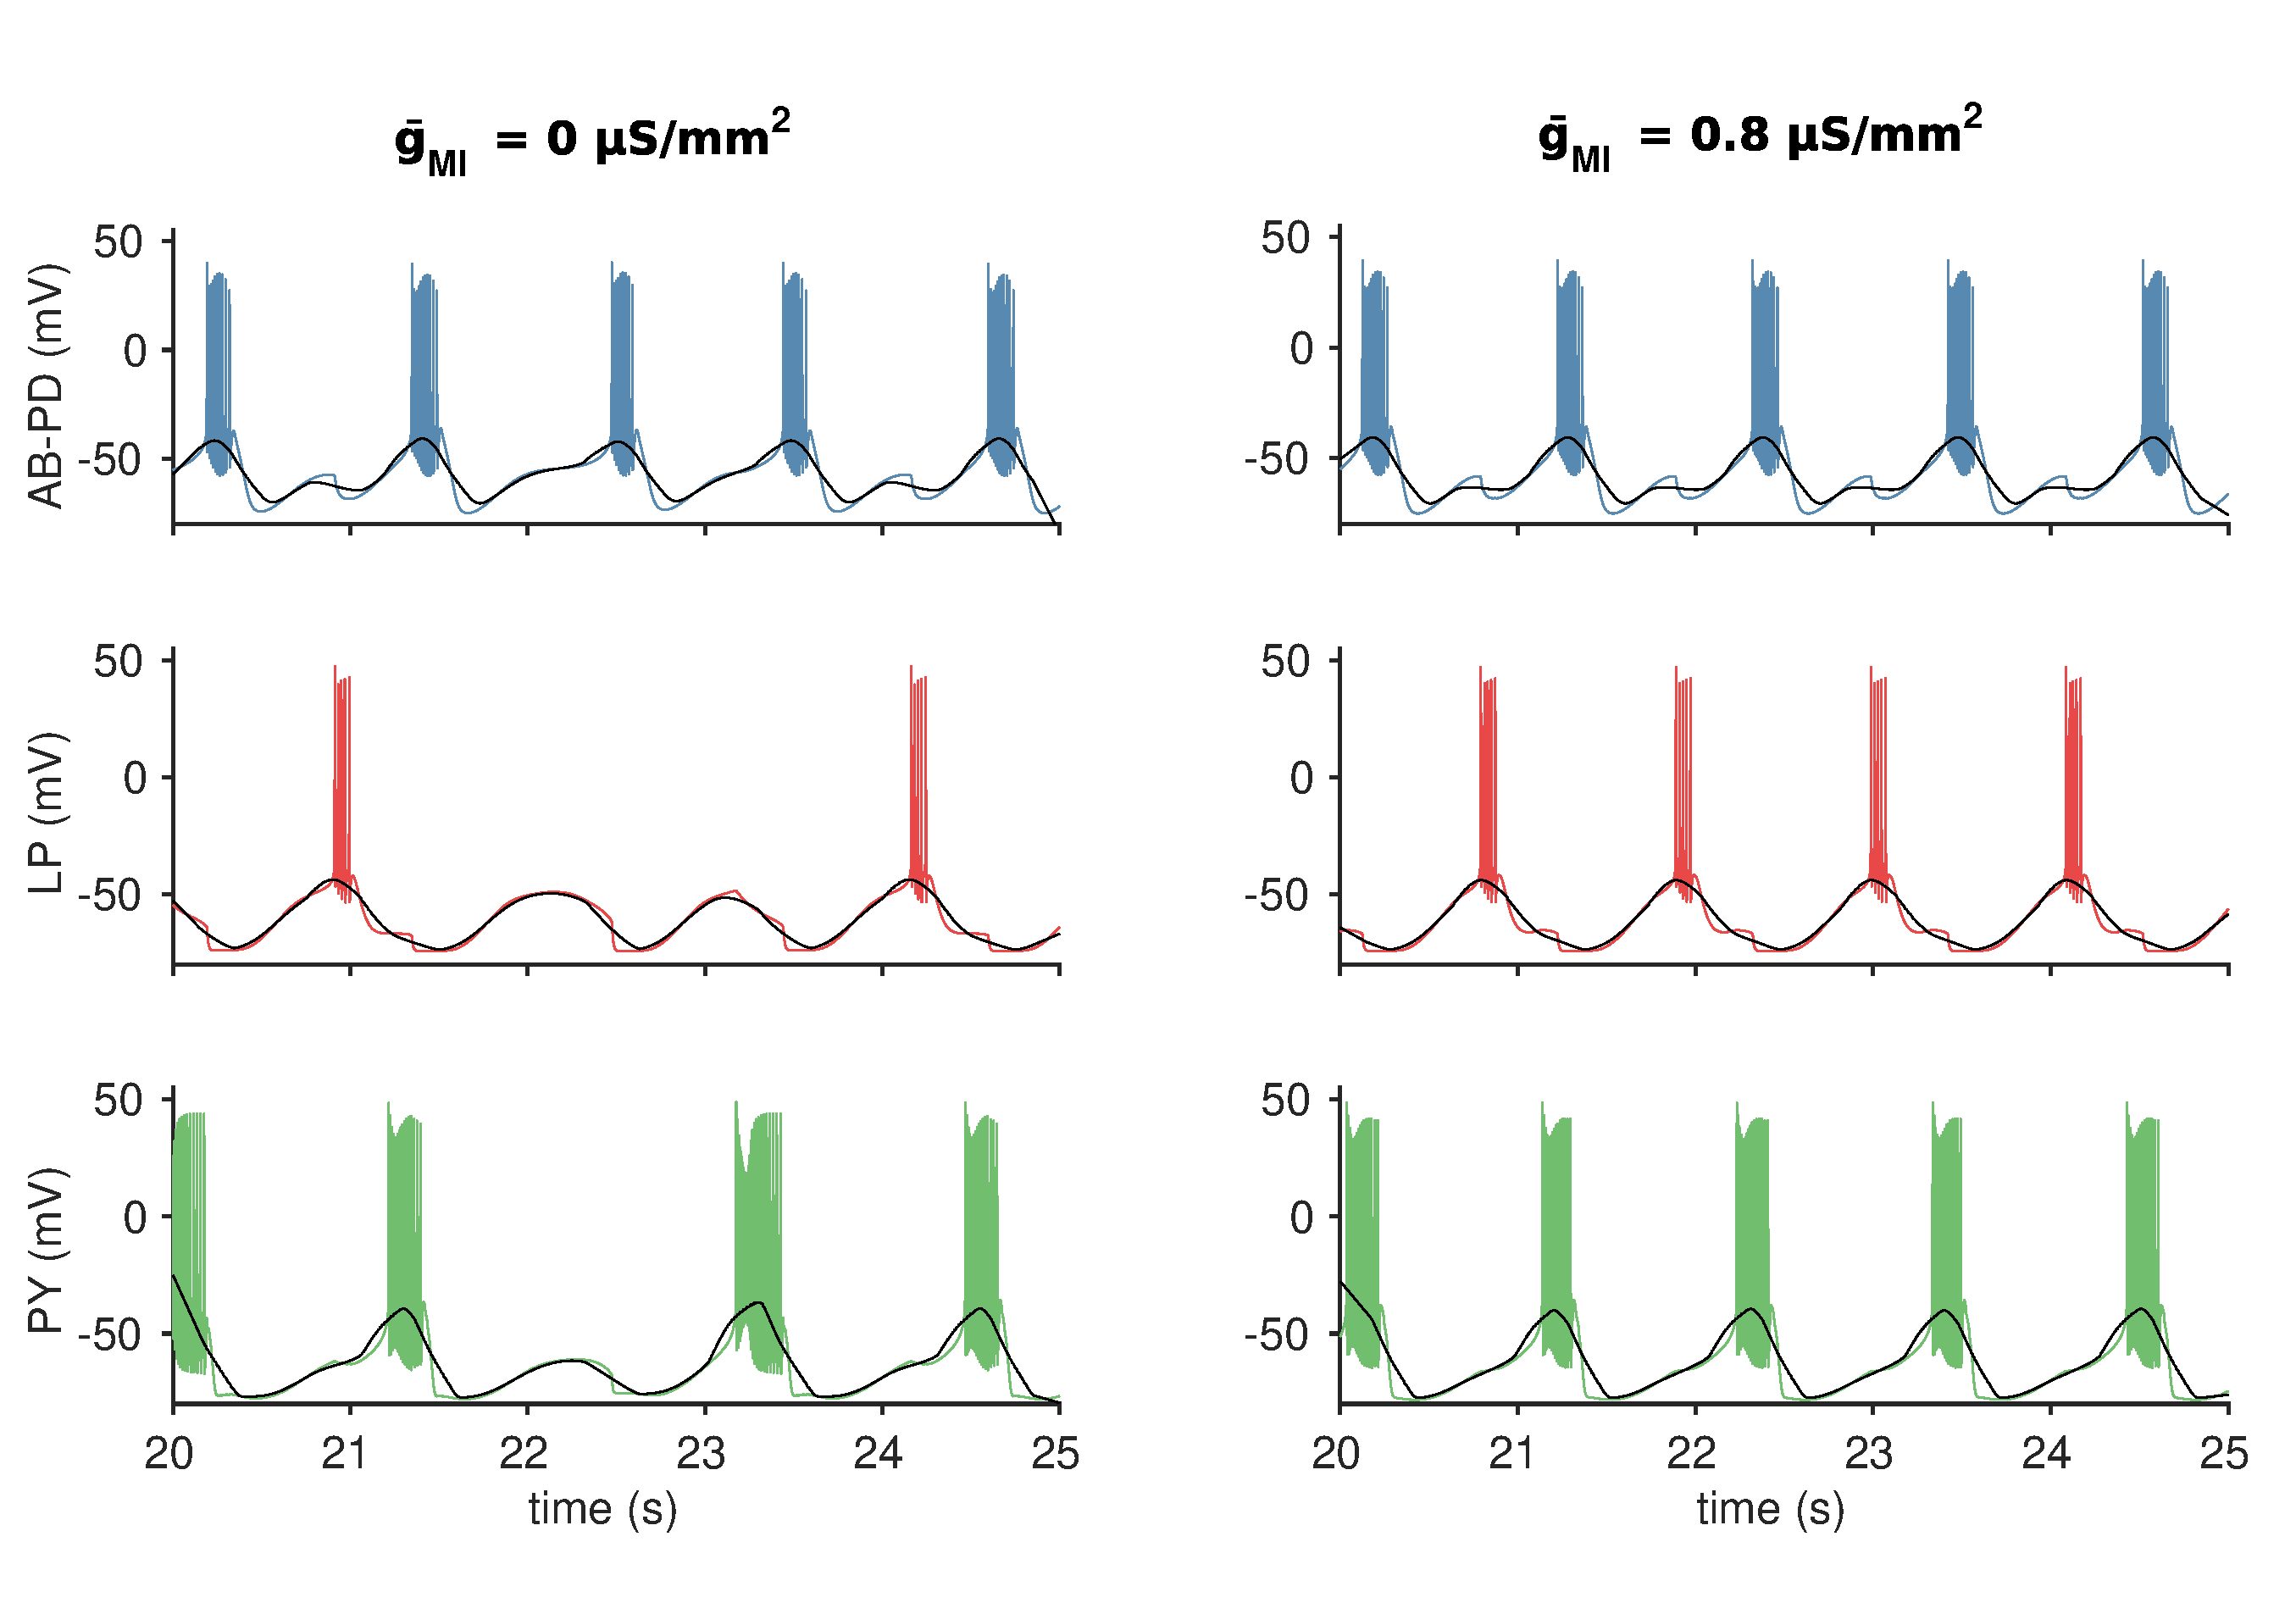
\includegraphics[width=1.0\linewidth]{gfx/network/network_LP_28_traces}
	\caption[Network with modulation into LP (traces)]{Modulation into \acs{LP} rescues abnormal activity. Modulation into \acs{LP} increases burst frequency and \acs{AB}-\acs{PD} slow wave amplitude. Left-hand traces are without neuromodulation. Right-hand traces have \acs{IMI} in \acs{LP} at $\bar{g}_{MI} = 0.8~\mu \mathrm{S/mm^2}$. Colors indicate cells (blue is \acs{AB}-\acs{PD}, red is \acs{LP}, green is \acs{PY} and overlaid black indicates the slow wave).}
	\label{fig:networklp28traces}
\end{figure}

\begin{figure}[h]
	\centering
	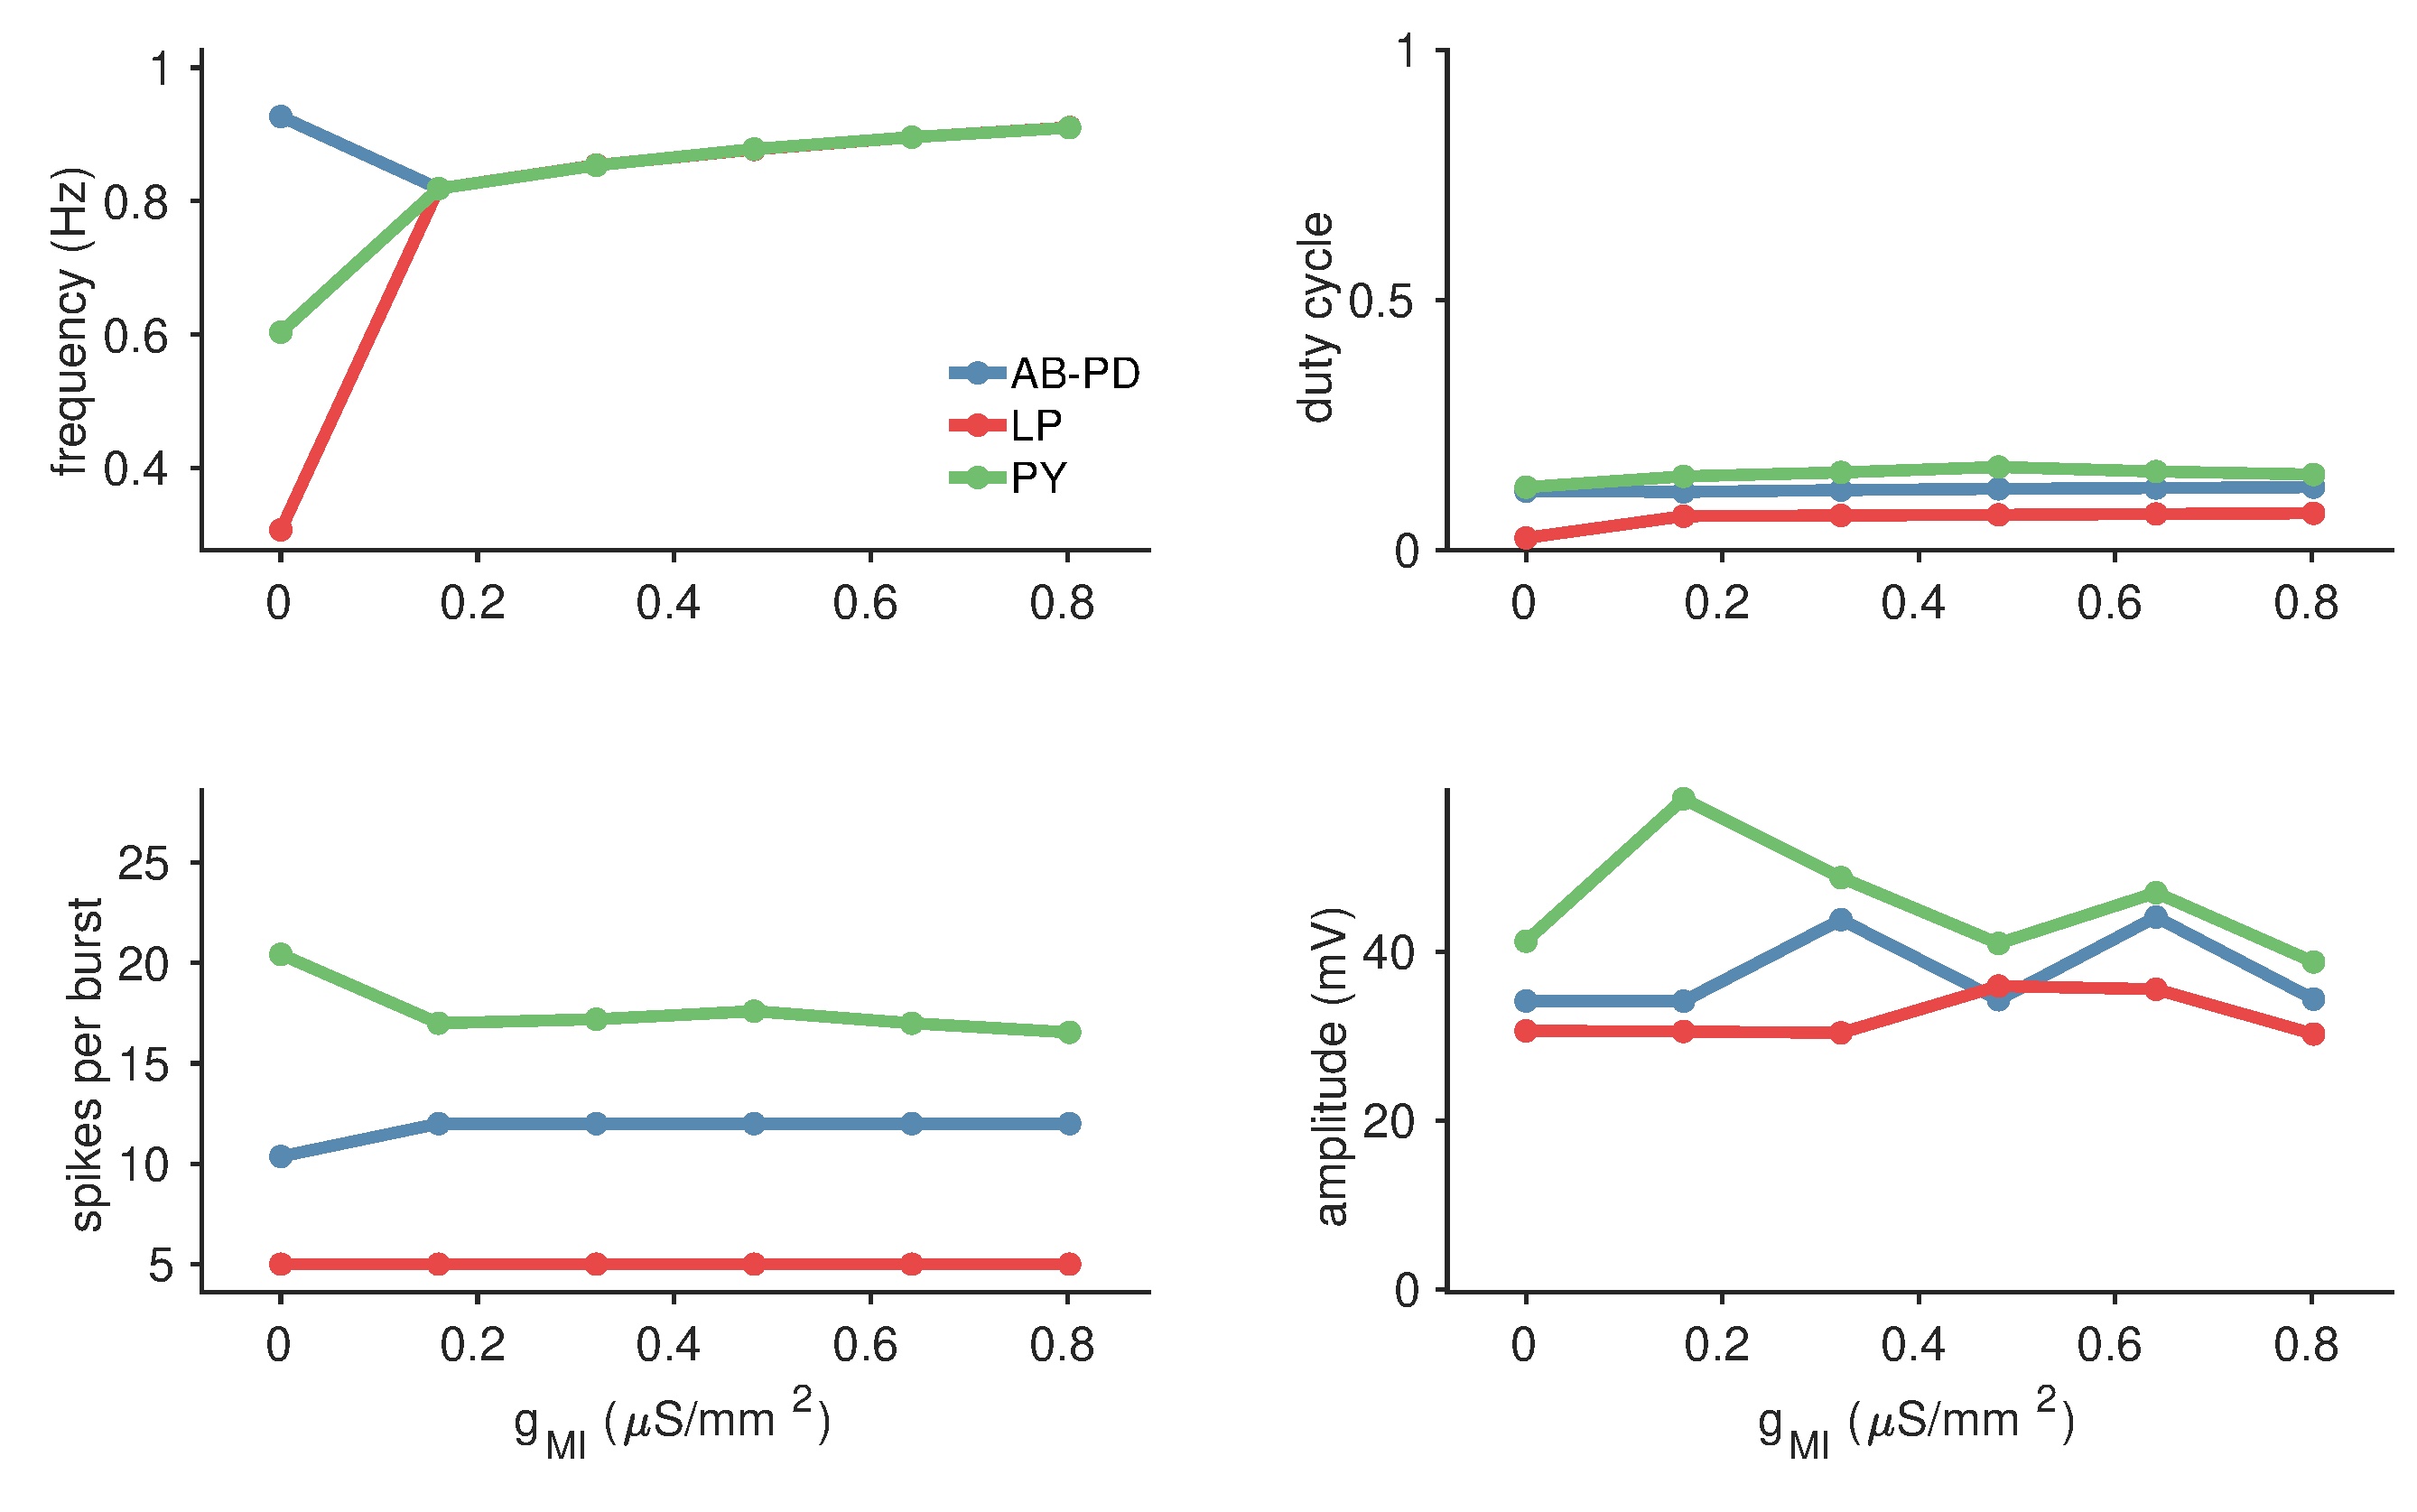
\includegraphics[width=1.0\linewidth]{gfx/network/network_LP_28_metrics}
	\caption[Network with modulation into LP (metrics)]{Modulation into \acs{LP} rescues abnormal activity. Modulation into \acs{AB}-\acs{PD} increases burst frequency and \acs{AB}-\acs{PD} slow wave amplitude. Metrics at steady-state as a function of increasing modulatory input. Colors indicate cells (blue is \acs{AB}-\acs{PD}, red is \acs{LP}, green is \acs{PY}).}
	\label{fig:networklp28metrics}
\end{figure}

\FloatBarrier

Models can recapitulate loss of triphasic rhythm with decentralization. In \autoref{fig:networklp28traces}, modulation into \acs{LP} corrects a network with burst asymmetry. After the network is brought back into rhythm, increasing modulation increases the burst frequency. Since all bursts are short in duration, the duty cycle does not change. The slow wave amplitude in \acs{AB}-\acs{PD} depends on the phase relationship between \acs{AB}-\acs{PD} and \acs{LP}, which itself depends on the maximal conductance of \acs{IMI} in \acs{LP}. When the burst in \acs{LP} occurs immediately following the termination of the burst in \acs{AB}-\acs{PD}, allowing more time between the termination of the burst in \acs{LP} and the next in \acs{AB}-\acs{PD} the amplitude in the pacemaker is greater.

\begin{figure}[h]
	\centering
	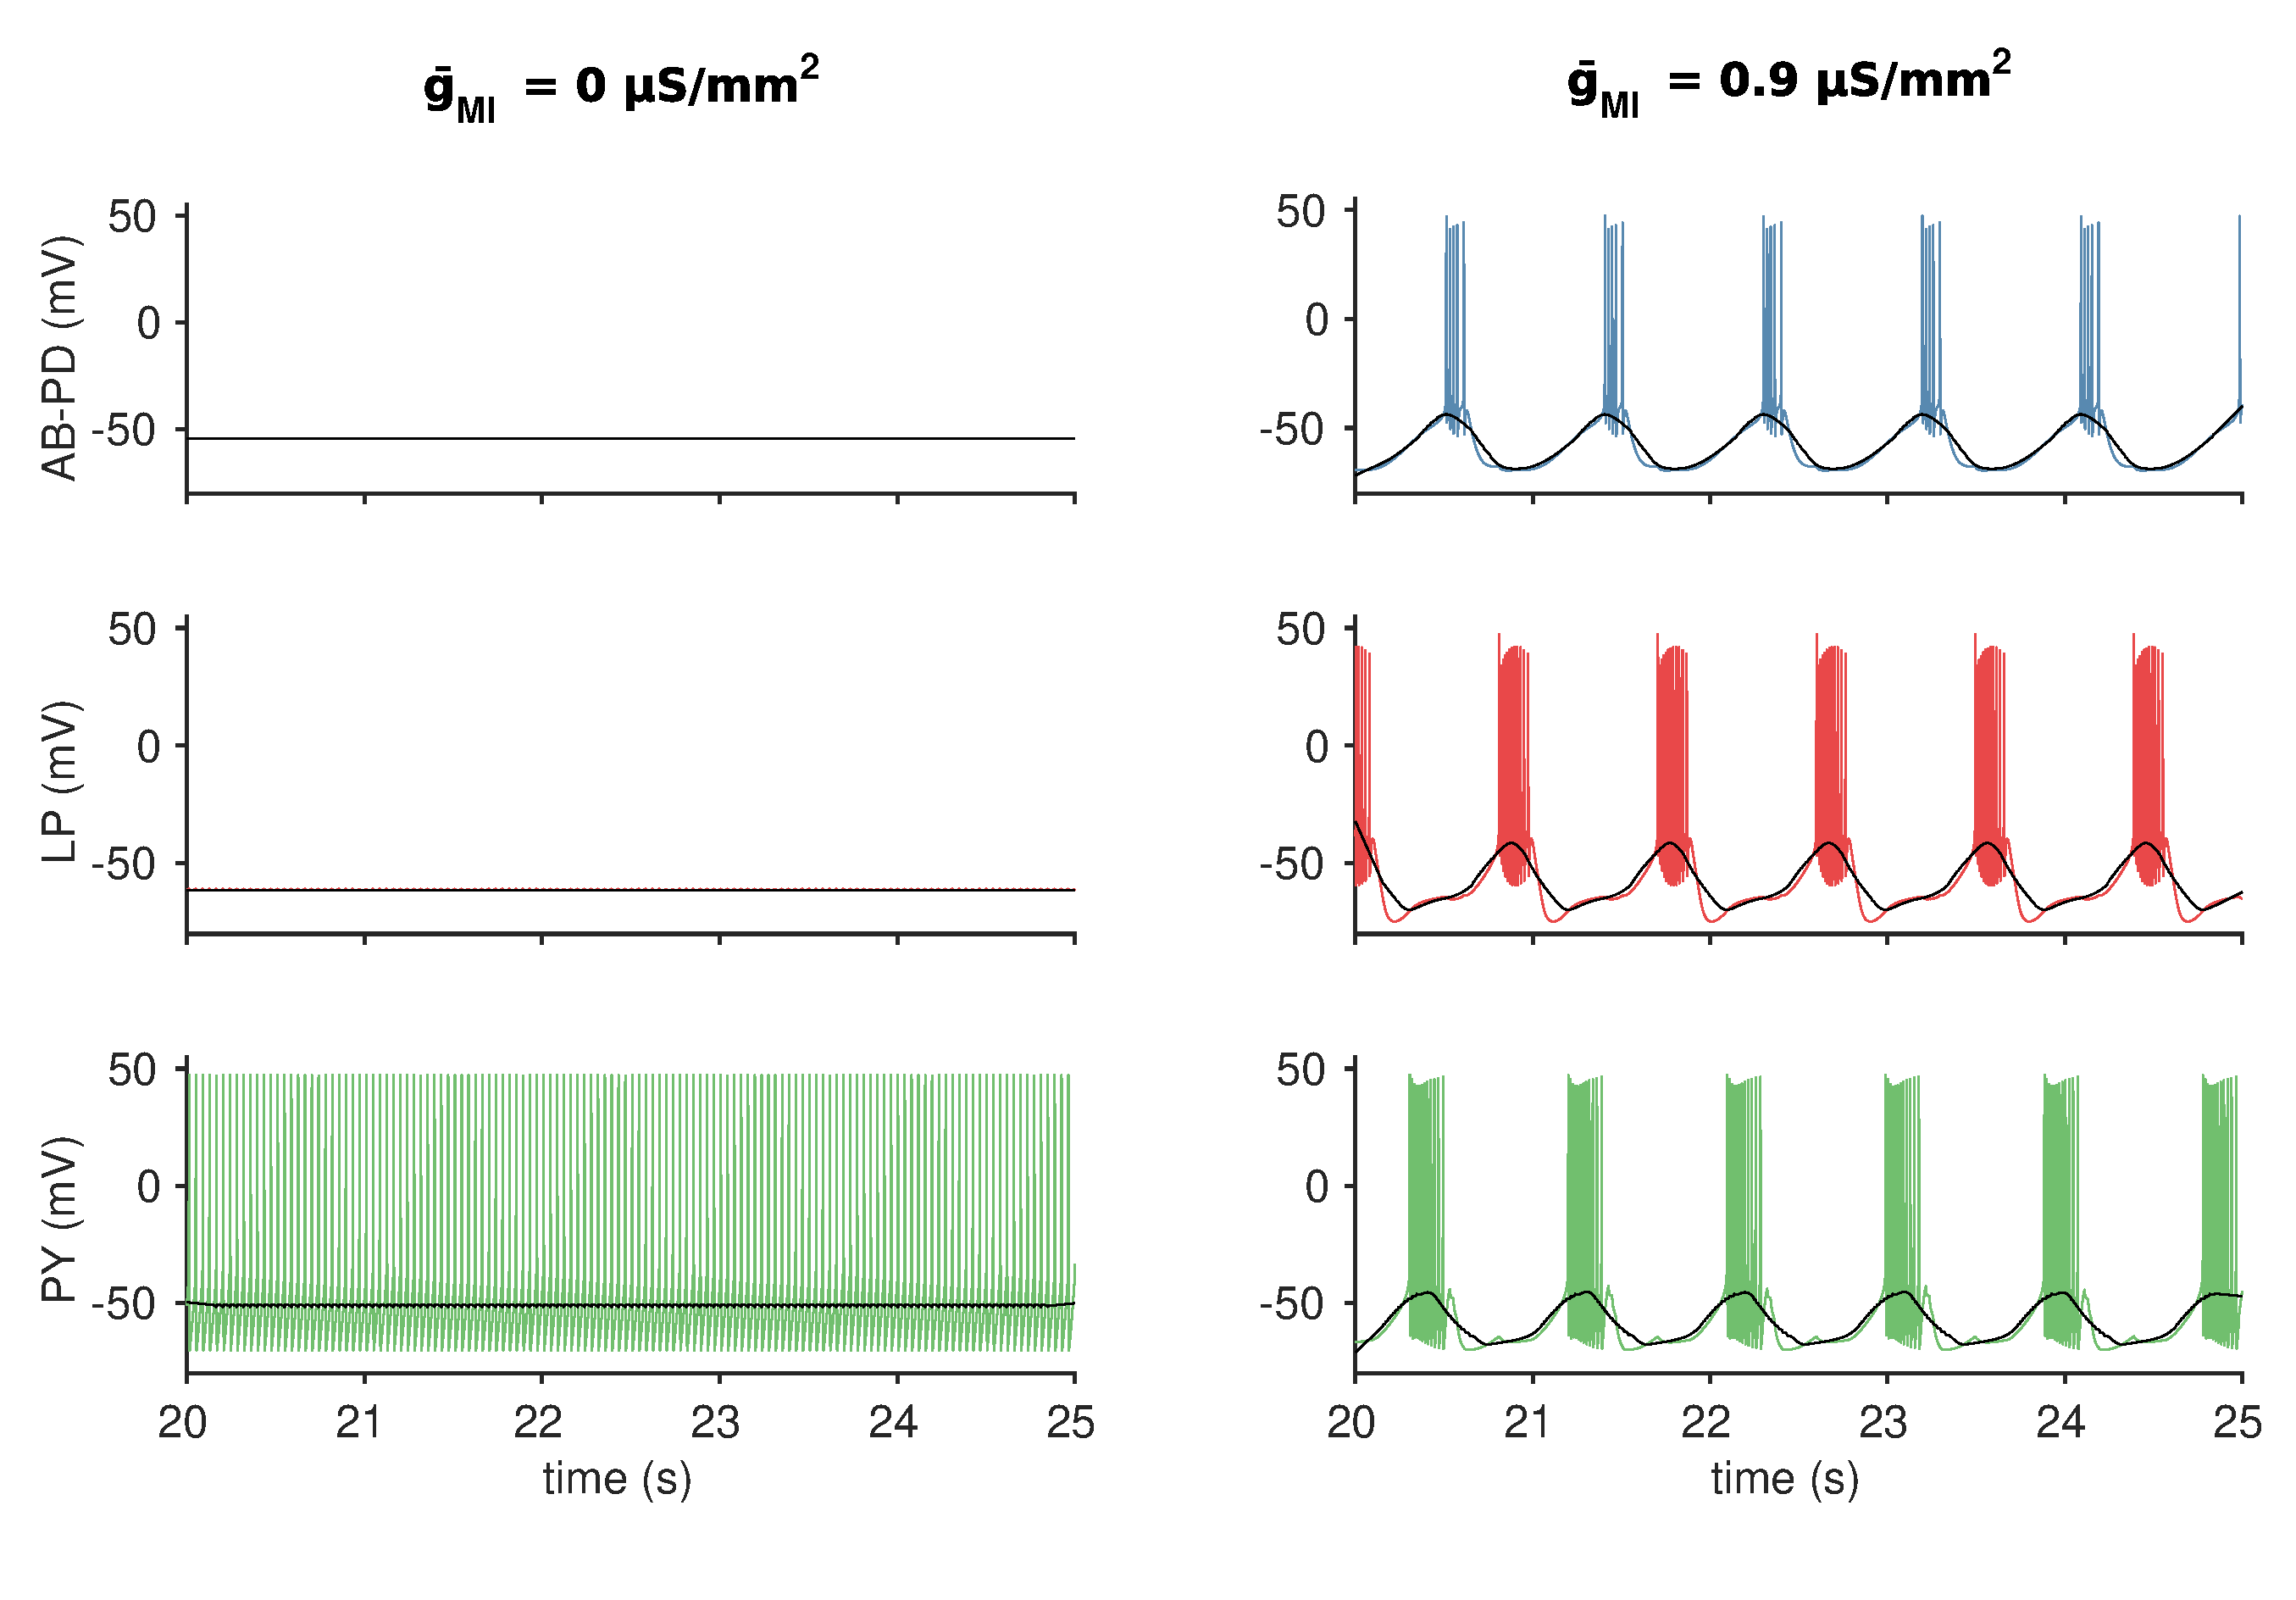
\includegraphics[width=1.0\linewidth]{gfx/network/network_AB_LP_14_traces}
	\caption[Network with modulation into AB-PD \& LP (traces)]{Modulation onto \acs{AB}-\acs{PD} produces triphasic network activity in a quiescent network model. Modulation of the pacemaker increases burst frequency and \acs{AB}-\acs{PD} slow wave amplitude. Left-hand traces are without neuromodulation.. Right-hand traces have \acs{IMI} in \acs{AB}-\acs{PD} at $\bar{g}_{MI} = 0.9~\mu \mathrm{S/mm^2}$. Colors indicate cells (blue is \acs{AB}-\acs{PD}, red is \acs{LP}, green is \acs{PY} and overlaid black indicates the slow wave).}
	\label{fig:networkablp14traces}
\end{figure}

\begin{figure}[h]
	\centering
	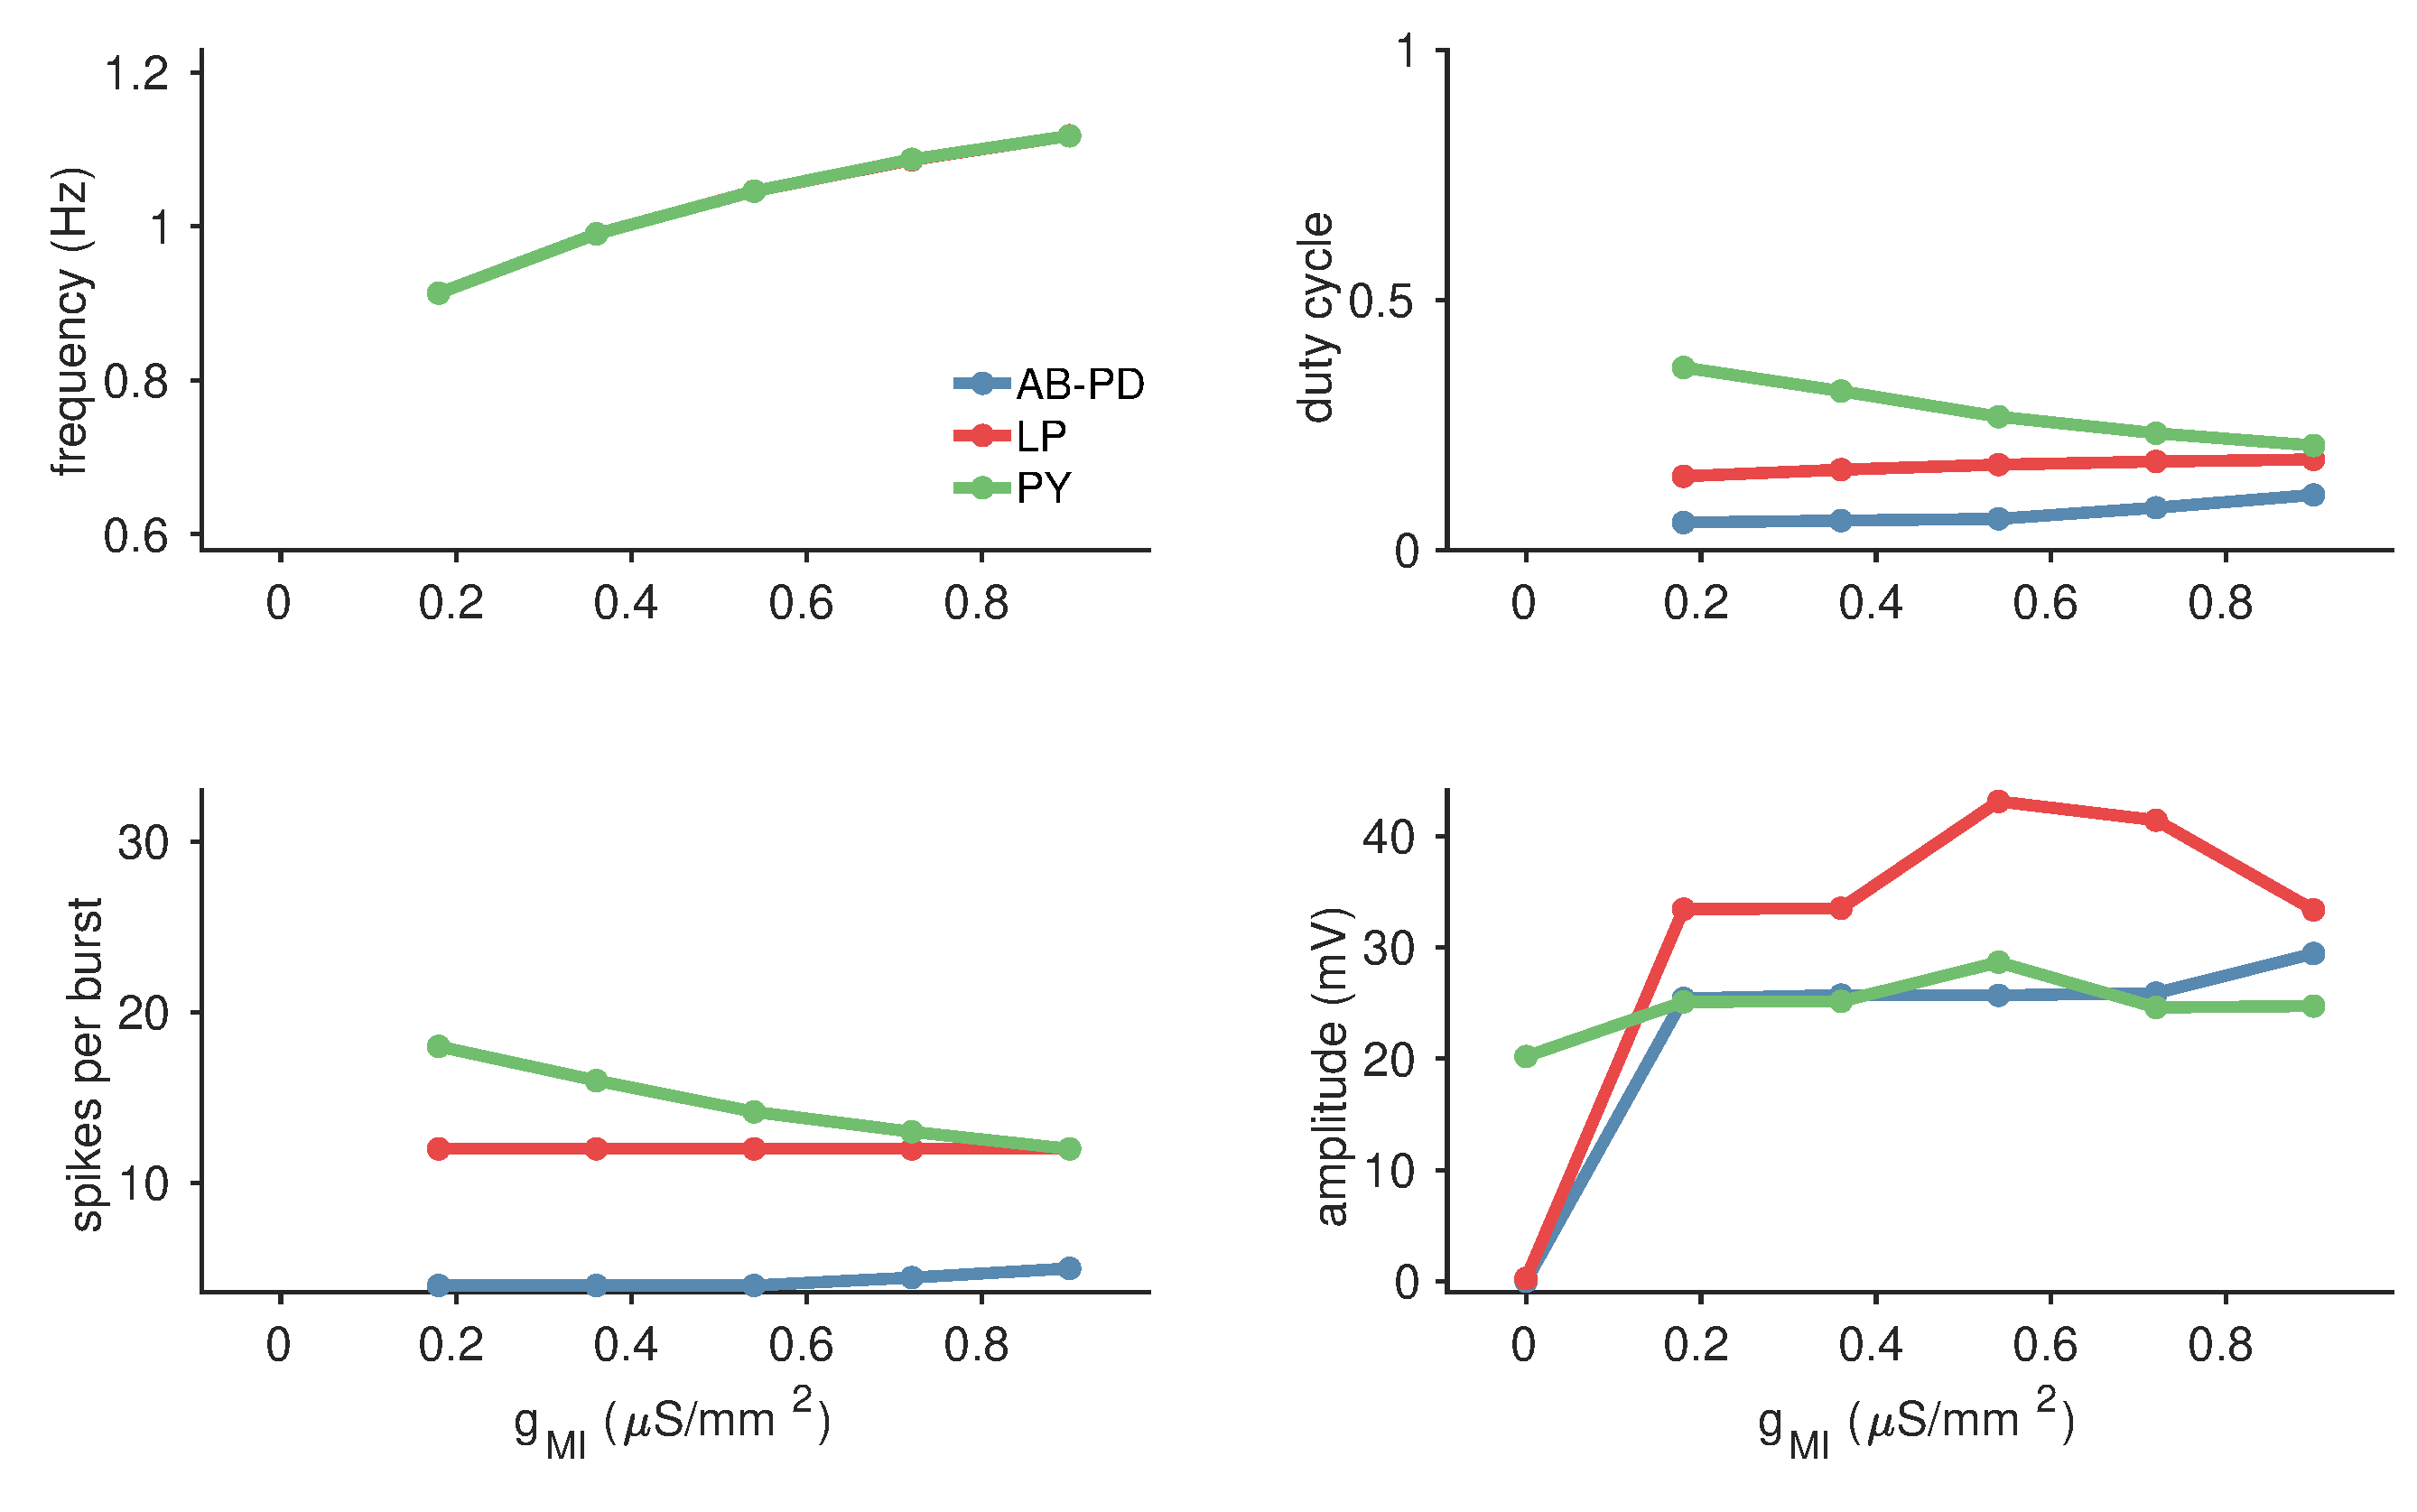
\includegraphics[width=1.0\linewidth]{gfx/network/network_AB_LP_14_metrics}
	\caption[Network with modulation into AB-PD \& LP (metrics)]{Modulation onto \acs{AB}-\acs{PD} produces triphasic network activity in a quiescent network model. Modulation of the pacemaker increases burst frequency and \acs{AB}-\acs{PD} slow wave amplitude. Metrics at steady-state as a function of increasing modulatory input. Colors indicate cells (blue is \acs{AB}-\acs{PD}, red is \acs{LP}, green is \acs{PY}).}
	\label{fig:networkablp14metrics}
\end{figure}

\FloatBarrier

\autoref{fig:networkablp14traces} shows quiescence in the decentralized state and normal triphasic activity with modulation in both the pacemaker and \acs{LP}. Monotonic increase in burst frequency and decrease in duty cycle for models above 0.3 can be seen here as well.

These models qualitatively reproduce slower, variable rhythms in decentralized preparations that recover with activation of \acs{IMI} in \acs{AB}, \acs{PD}, or \acs{LP}.

\FloatBarrier

\subsection{Modulation of AB-PD and LP Promotes Robust Pyloric Rhythms}

Modulatory input conductance was applied to \acs{AB}-\acs{PD} and \acs{LP} model neurons separately and together at differing strengths. Of the 146 models examined, 87 were optimized for pacemaker modulation, 29 for \acs{LP} modulation, and 30 for \acs{IMI} in \acs{AB}-\acs{PD} and \acs{LP}. When models which were triphasic during decentralization were removed, more networks recovered pyloric rhythmicity under modulation of the pacemaker and \acs{LP} than the pacemaker or \acs{LP} alone (\autoref{fig:allstats}).



\begin{figure}
	\centering
	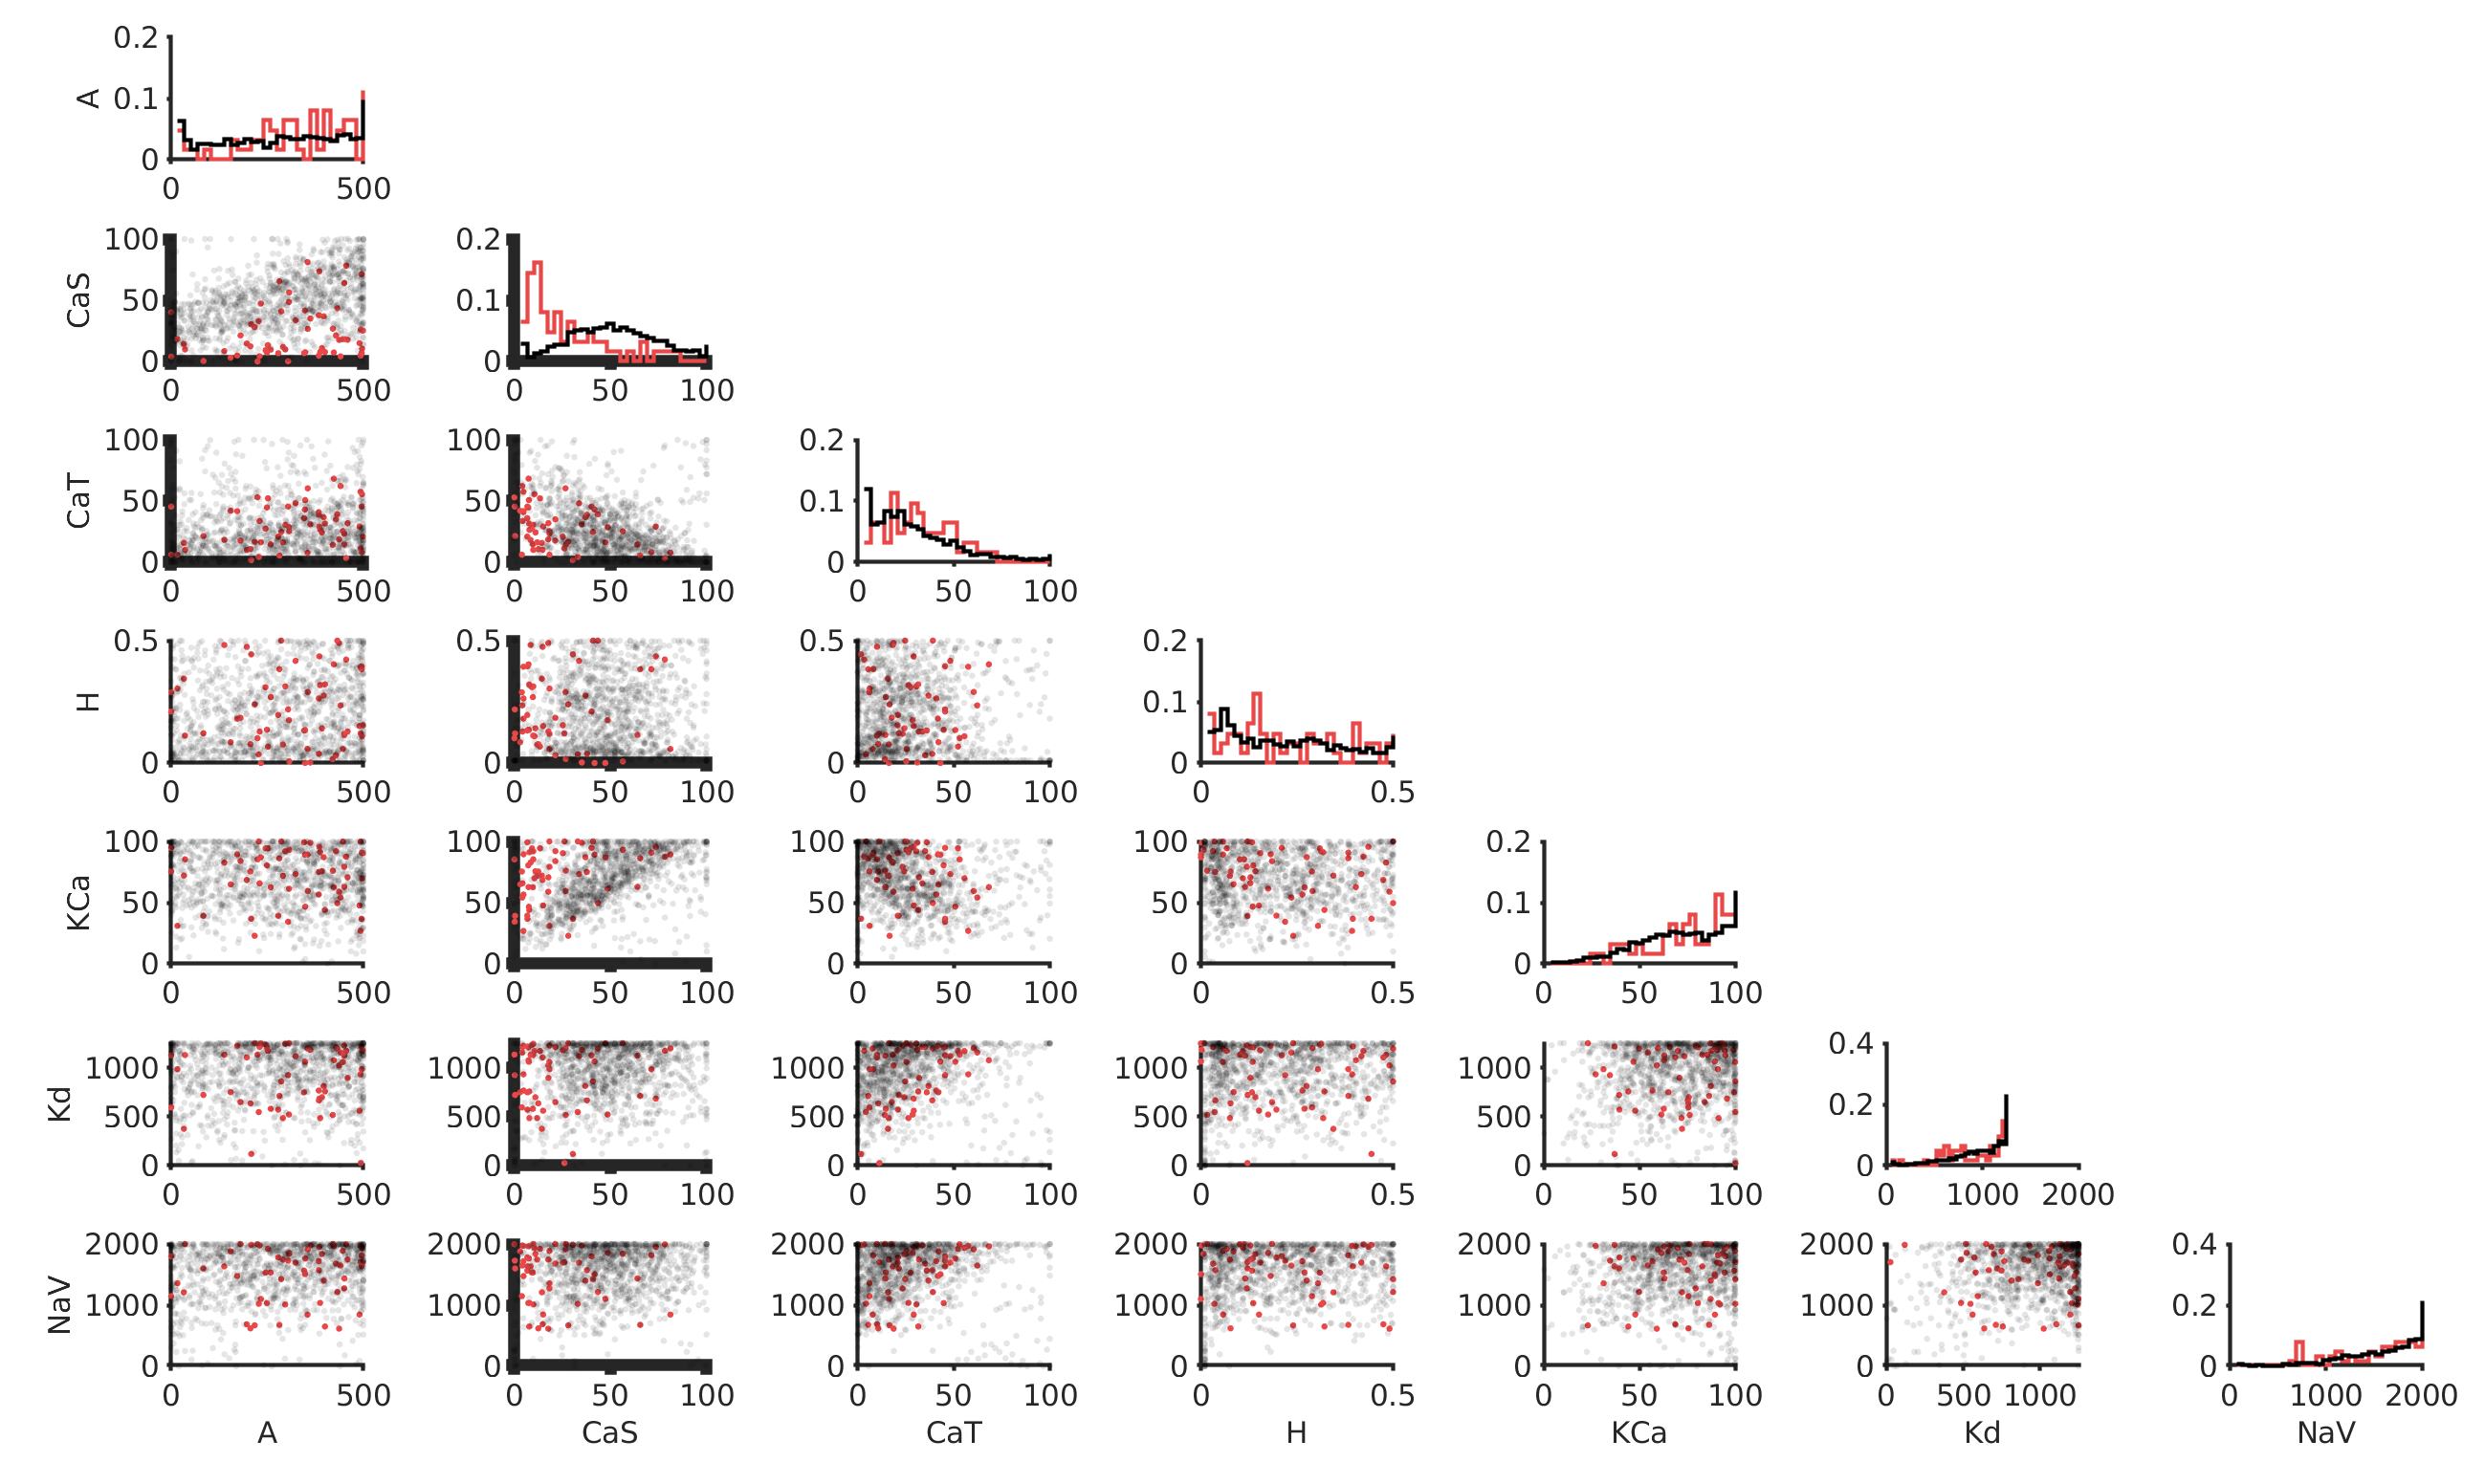
\includegraphics[width=1.3\linewidth]{gfx/all-modulation/correlations_AB}
	\caption[Cross-correlations in AB-PD model maximal conductances]{Cross-correlation in \acs{AB}-\acs{PD} maximal conductances from network models. Maximal conductances from control networks (black, $n=1,148$), which are pyloric in decentralized conditions, and optimized models (red, $n=82$), which are non-pyloric in decentralized conditions and pyloric under modulation onto \acs{AB}-\acs{PD} and \acs{LP}, are plotted against each other. Plots on the diagonal are histograms of maximal conductance. normalized to population size in each case. \textbf{Bold} axes indicate significant correlation (Kolmogorov-Smirnov 2-tailed 2-D test, $p<0.05$). All conductances are in $\mu\mathrm{S/mm^2}.$}  
	\label{fig:correlationsab}
\end{figure}

\begin{figure}
	\centering
	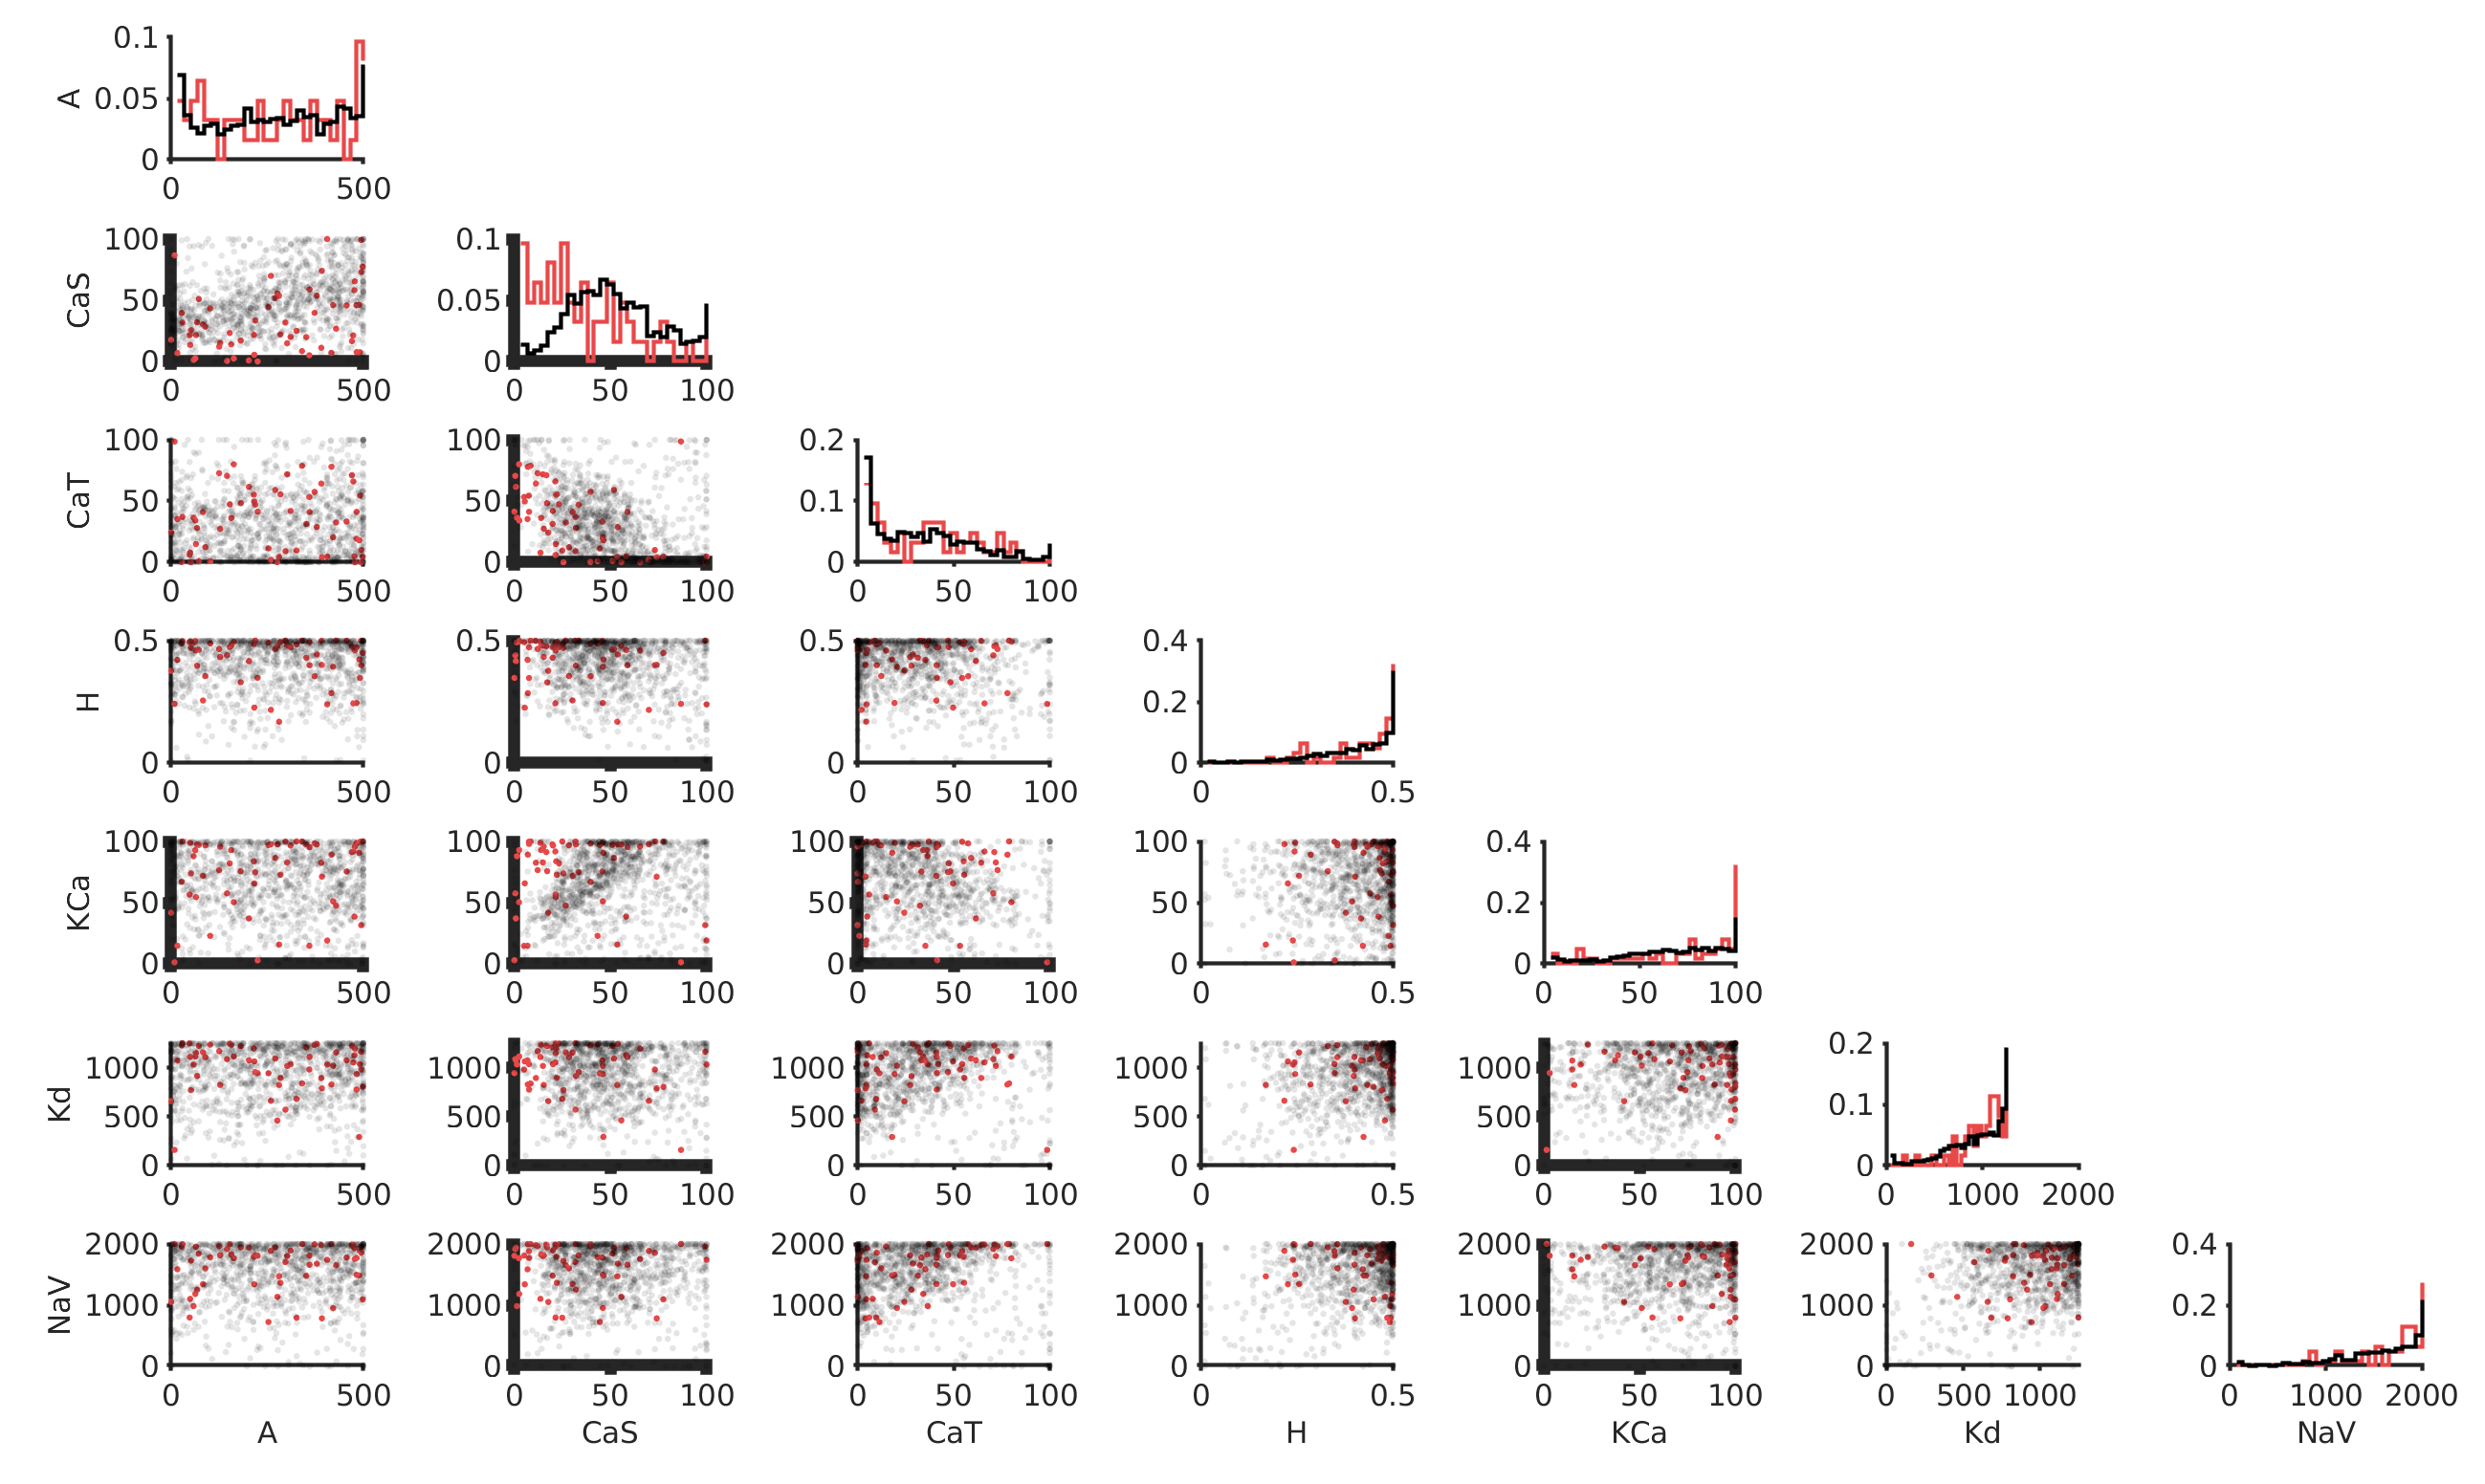
\includegraphics[width=1.3\linewidth]{gfx/all-modulation/correlations_LP}
	\caption[Cross-correlations in LP model maximal conductances]{Cross-correlation in \acs{LP} maximal conductances from network models. Maximal conductances from control networks (black, $n=1,148$), which are pyloric in decentralized conditions, and optimized models (red, $n=82$), which are non-pyloric in decentralized conditions and pyloric under modulation onto \acs{AB}-\acs{PD} and \acs{LP}, are plotted against each other. Plots on the diagonal are histograms of maximal conductance. normalized to population size in each case. \textbf{Bold} axes indicate significant correlation (Kolmogorov-Smirnov 2-tailed 2-D test, $p<0.05$). All conductances are in $\mu\mathrm{S/mm^2}.$}  
	\label{fig:correlationslp}
\end{figure}

\begin{figure}
	\centering
	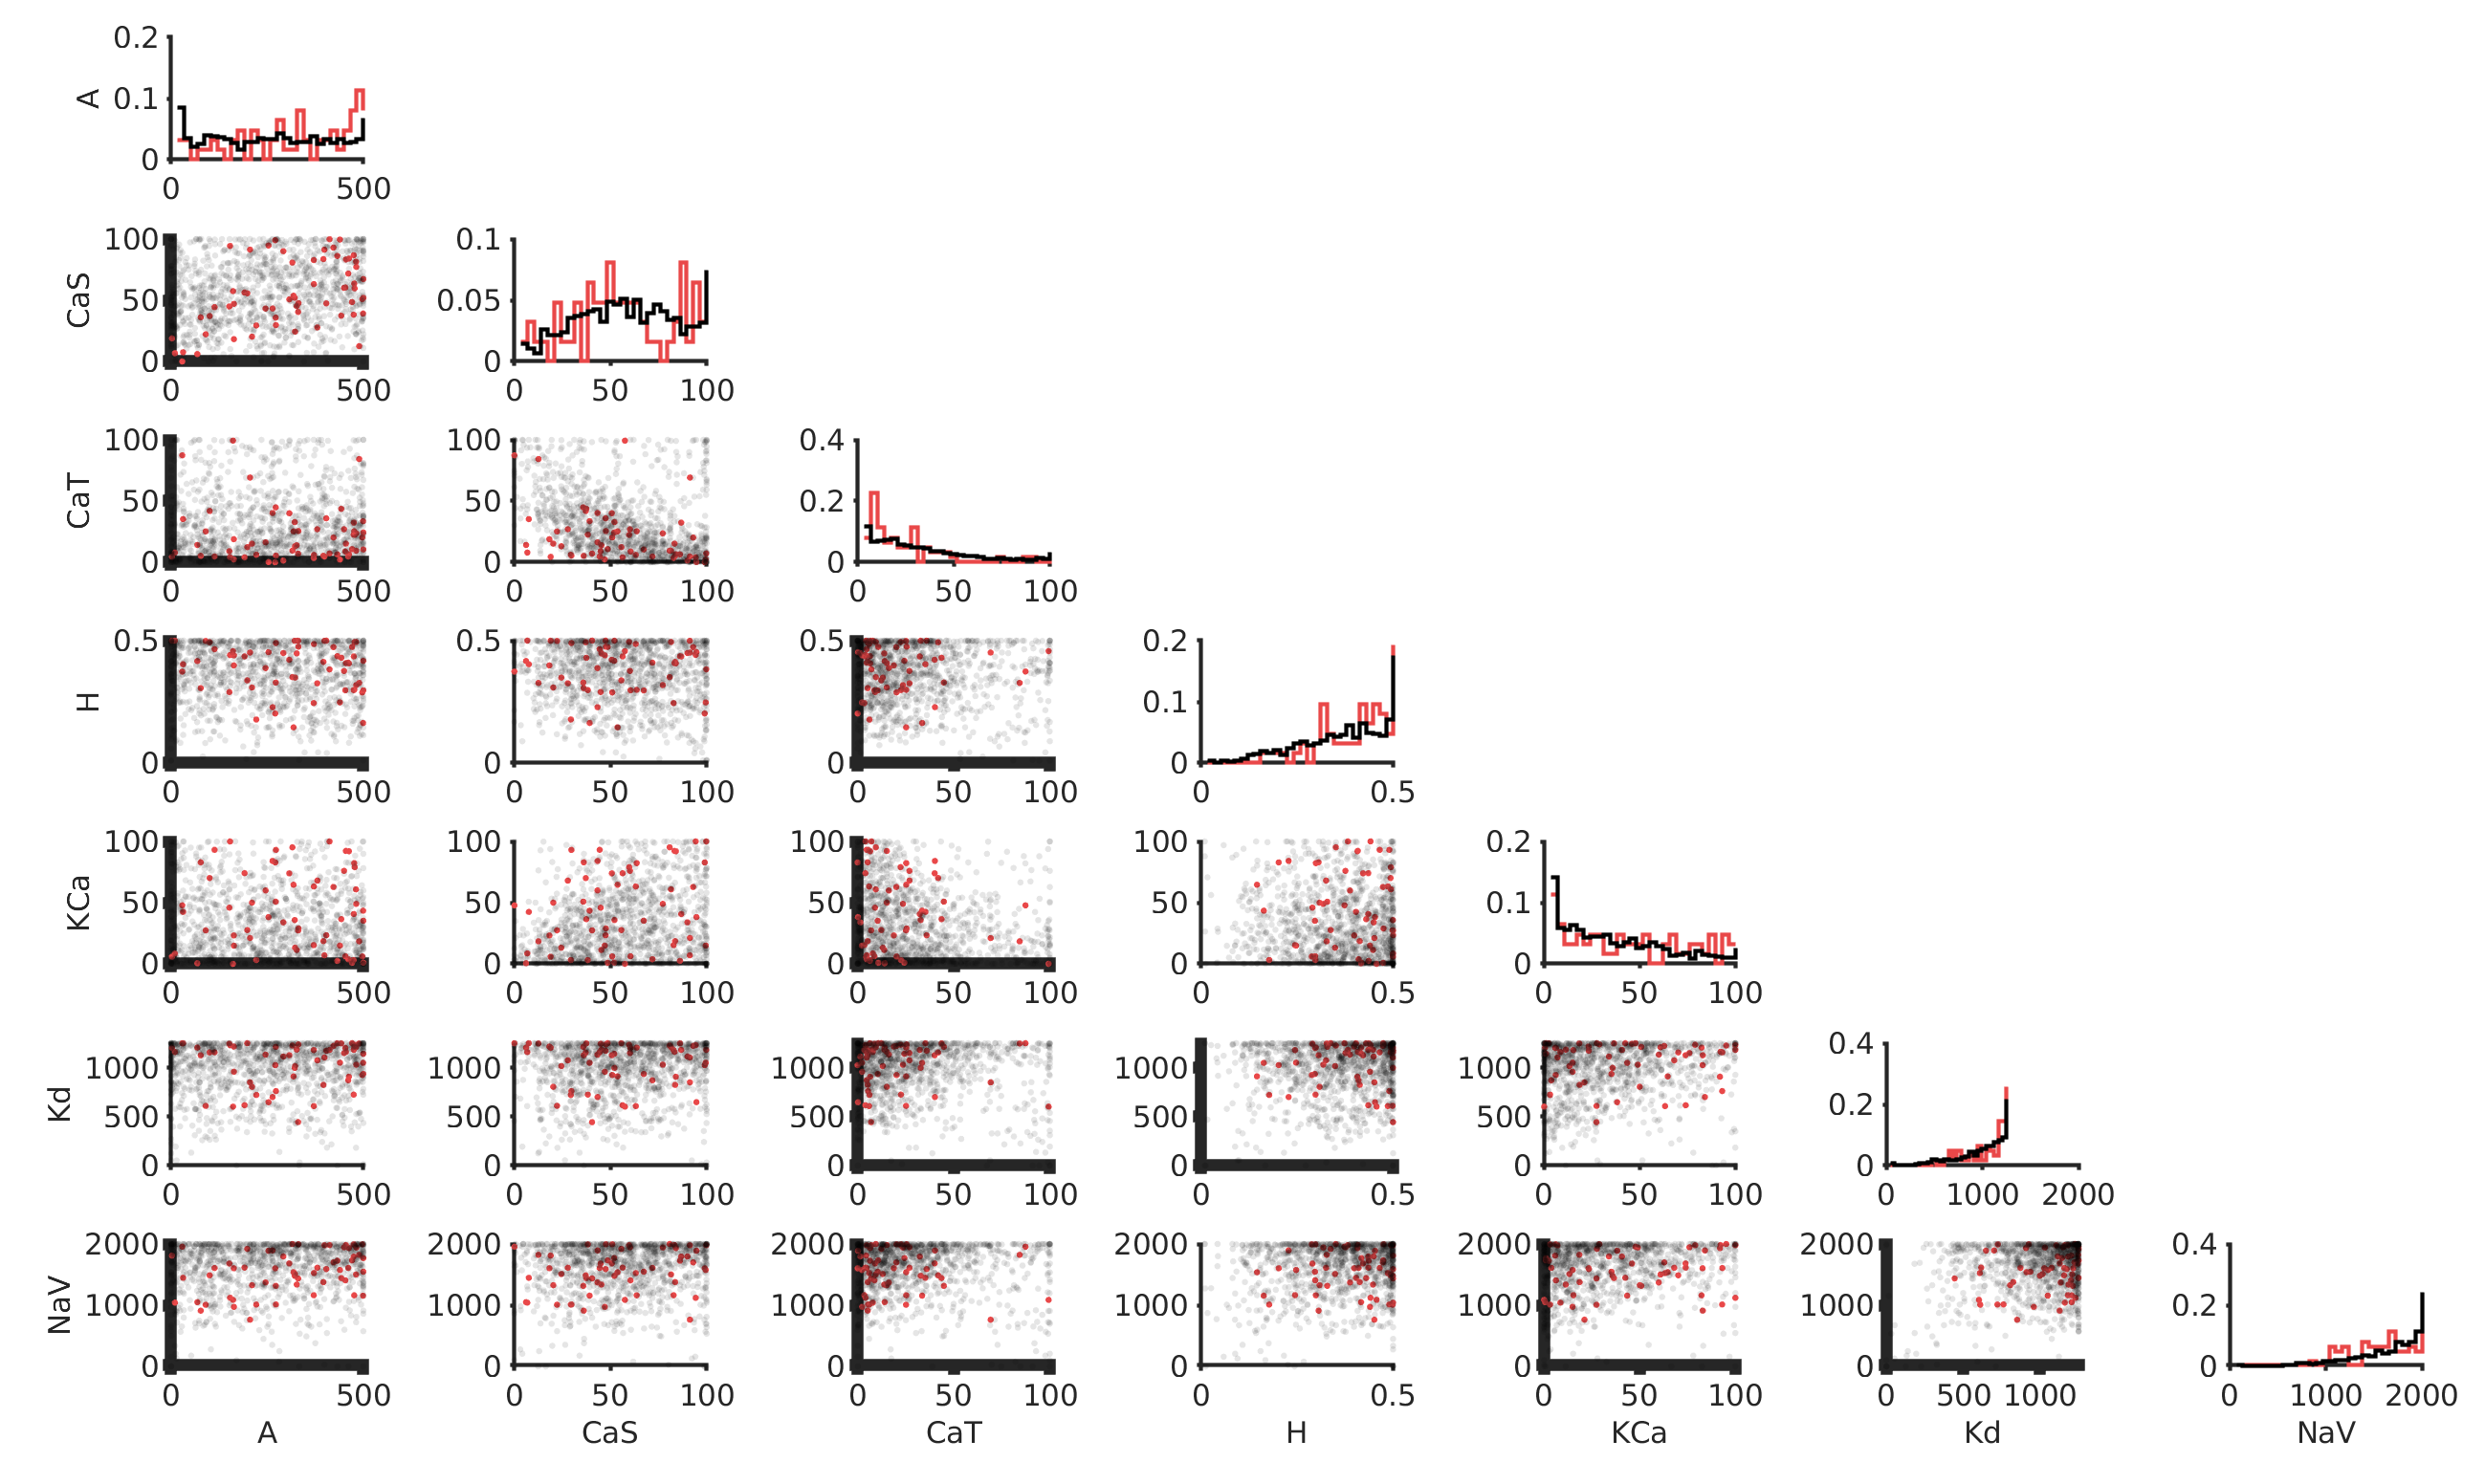
\includegraphics[width=1.3\linewidth]{gfx/all-modulation/correlations_PY}
	\caption[Cross-correlations in PY model maximal conductances]{Cross-correlation in \acs{PY} maximal conductances from network models. Maximal conductances from control networks (black, $n=1,148$), which are pyloric in decentralized conditions, and optimized models (red, $n=82$), which are non-pyloric in decentralized conditions and pyloric under modulation onto \acs{AB}-\acs{PD} and \acs{LP}, are plotted against each other. Plots on the diagonal are histograms of maximal conductance. normalized to population size in each case. \textbf{Bold} axes indicate significant correlation (Kolmogorov-Smirnov 2-tailed 2-D test, $p<0.05$). All conductances are in $\mu\mathrm{S/mm^2}.$}  
	\label{fig:correlationspy}
\end{figure}

\begin{figure}
	\centering
	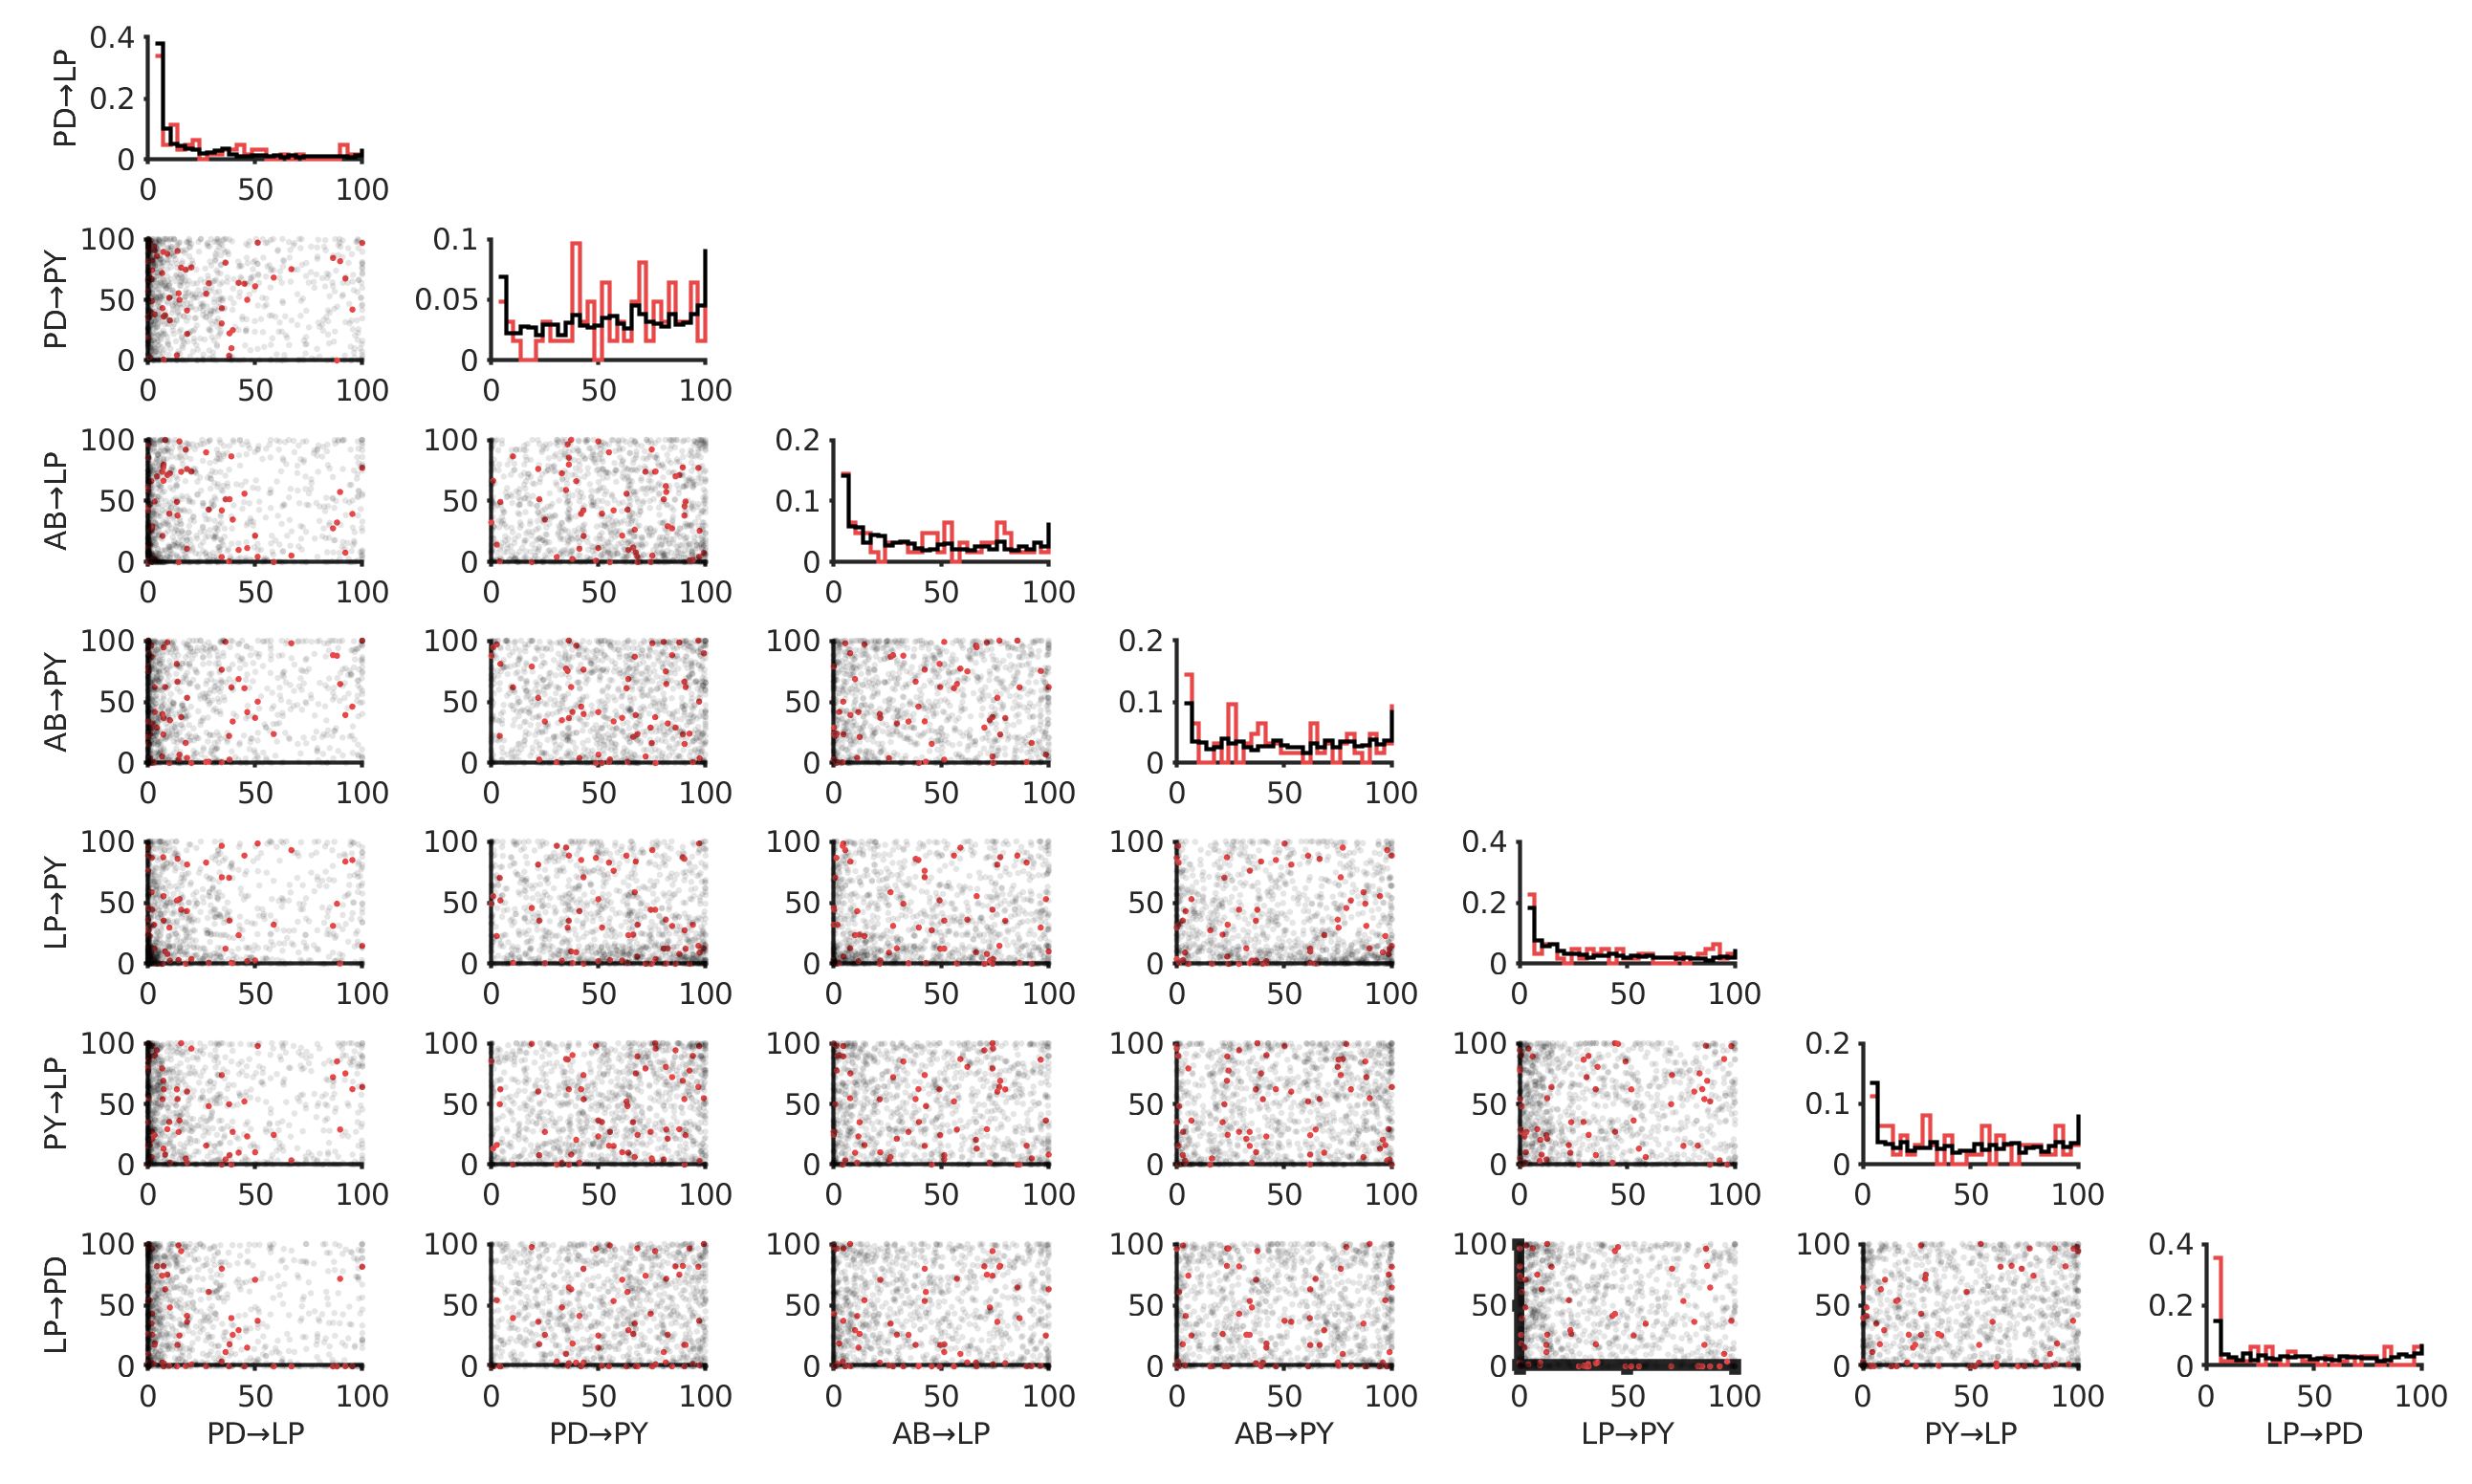
\includegraphics[width=1.3\linewidth]{gfx/all-modulation/correlations_synapses}
	\caption[Cross-correlations in synaptic maximal conductances]{Cross-correlation in synaptic maximal conductances from network models. Arrows point from presynaptic to post-synaptic neurons. All synapses are inhibitory and glutamatergic except for synapses from \acs{PD} which are cholinergic. Maximal conductances from control networks (black, $n=1,148$), which are pyloric in decentralized conditions, and optimized models (red, $n=82$), which are non-pyloric in decentralized conditions and pyloric under modulation onto \acs{AB}-\acs{PD} and \acs{LP}, are plotted against each other. Plots on the diagonal are histograms of maximal conductance. normalized to population size in each case. \textbf{Bold} axes indicate significant correlation (Kolmogorov-Smirnov 2-tailed 2-D test, $p<0.05$). All conductances are in $\mu\mathrm{S/mm^2}.$} 
	\label{fig:correlationssynapses}
\end{figure}


We hypothesized that this effect is caused by the effectiveness of post-inhibitory rebound as a mechanism for stabilization of central patterns. \acs{AB}-\acs{PD} and \acs{LP} mutually inhibit each other. Phasic excitation applied to each network component during the rising phase of the slow wave would then drive the network through enhanced mutual inhibition.

\begin{figure}
	\centering
	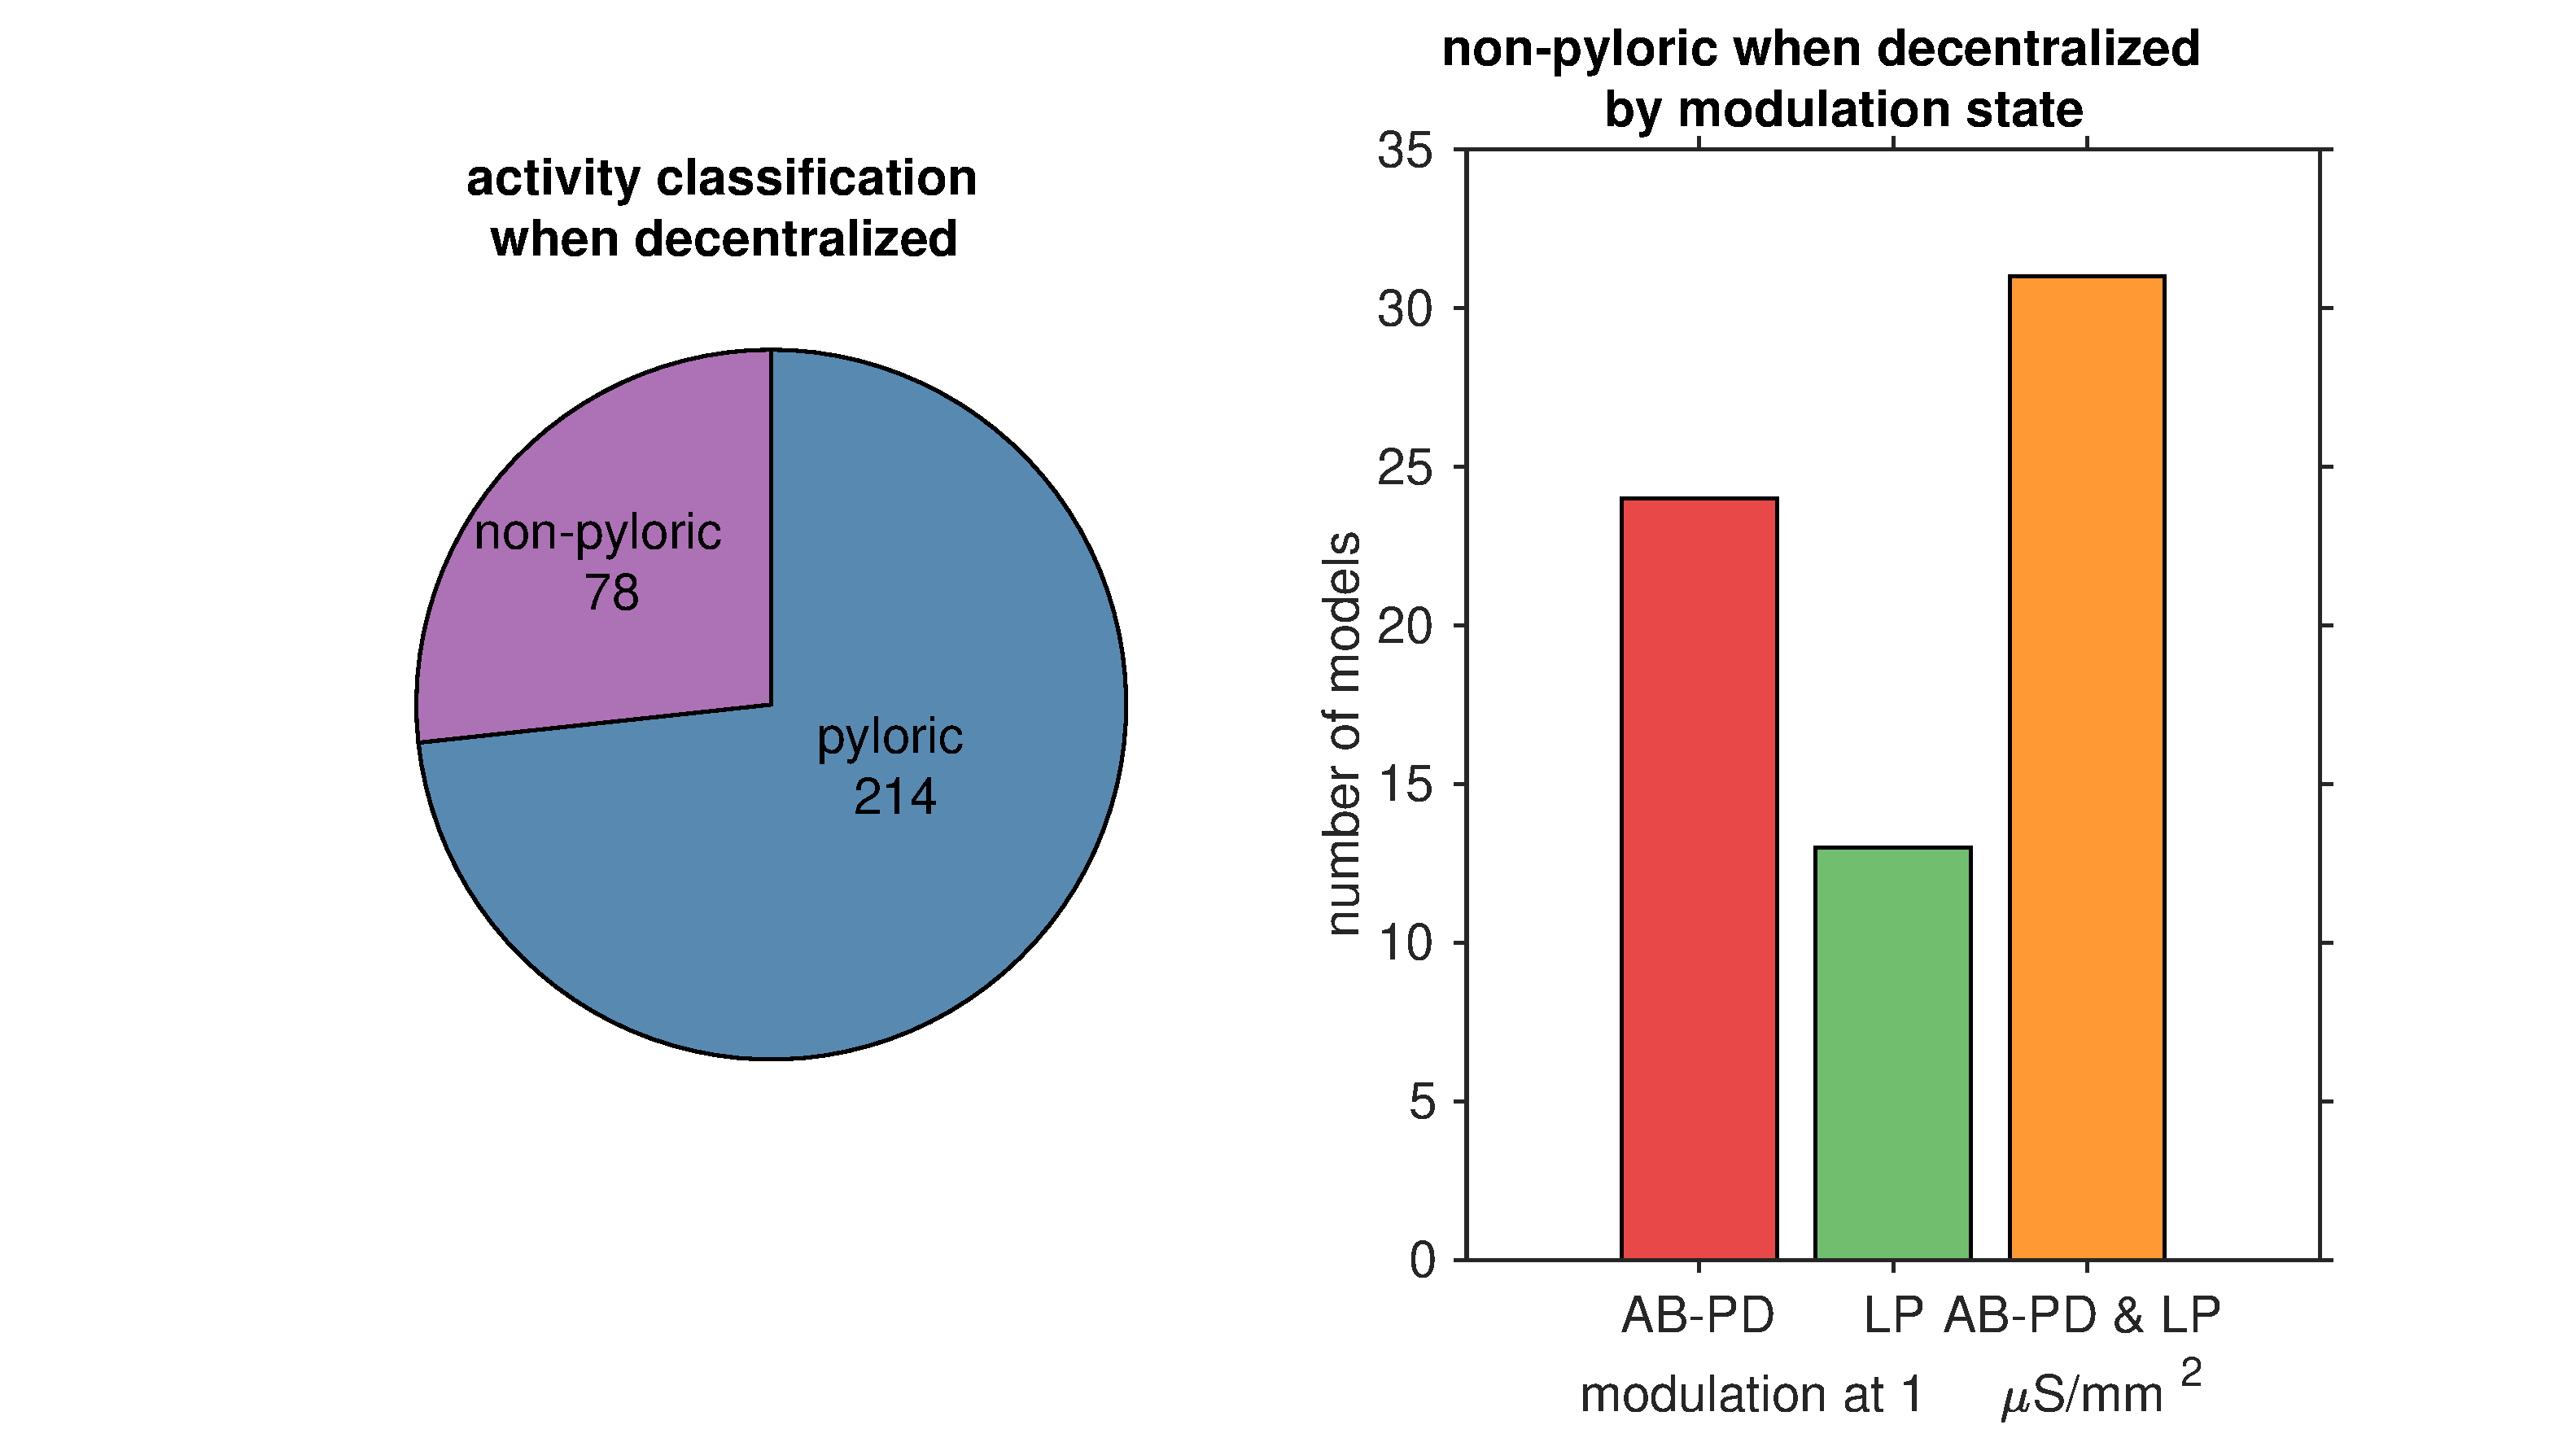
\includegraphics[width=1.0\linewidth]{gfx/all-modulation/all_stats}
	\caption[Distribution of rhythmicity in network models]{Distribution of triphasic network models by modulation state ($n=146$). \textit{Left:} Most triphasic models have \acs{IMI} in the pacemaker kernel and \acs{LP}, representing intact descending modulation, though many optimized models are triphasic in the decentralized state. This is due to optimization selecting for pyloric-like models \textit{prima facie}. \textit{Right:} When models which are triphasic in the decentralized state are excluded, most parameter sets result in triphasic networks with modulation and aberrant networks when decentralized.}
	\label{fig:allstats}
\end{figure}

The role of \acs{AB} and \acsp{PD} as the pacemaker kernel is recapitulated in these models. Modulation onto \acs{AB}-\acs{PD} more strongly drives network activity than modulation onto \acs{LP}. Models were classified as pyloric or non-pyloric in the four cases of modulation (decentralized, \acs{AB}-\acs{PD}, \acs{LP}, both). Correlations between classified network activity in these states reveals strong correlation between \acs{AB}-\acs{PD} and \acs{AB}-\acs{PD} \& \acs{LP} modulation states (\autoref{tab:correlations}).

To identify specific conductances important in models which respond to \acs{IMI}, correlations between maximal conductances from model networks which were non-pyloric in decentralized conditions, and pyloric with \acs{IMI} in \acs{AB}-\acs{PD} and \acs{LP} were computed. The 1,148 pyloric models from which the 146 networks were optimized for response to modulatory input were use as control data (\autoref{sec:parameteroptimization}). Maximal conductances for the three model neurons and seven synapses were plotted in cross-correlation diagrams (\autoref{fig:correlationsab}, \autoref{fig:correlationslp}, \autoref{fig:correlationspy}, \autoref{fig:correlationssynapses}). 

Two-sample, two-tailed two-dimensional Kolmogorov-Smirnov tests were used to determine significance\autocite{PeacockTwodimensionalgoodnessoffittesting1983}. Significant correlations were found between \acs{ICas} and all other conductances ($p < 0.05$) in \acs{AB}-\acs{PD} models. We hypothesize that since slow-wave calcium is responsible for burst propagation, models with low slow-calcium conductance are more responsive to neuromodulation in the form of \acs{IMI}, an inward current which activates near the peak of the slow wave. \acs{LP} model neurons also show reduced slow-wave calcium maximal conductance in comparison to the control networks. In addition, low \acs{ICaS} co-occurs with high \acs{IKCa} and \acs{IH}. \acs{IKCa} activates during burst termination and \acs{IH} rectifies hyperpolarization. Strong after-burst hyperpolarization, coupled with modulation- and \acs{IH}-mediated recovery would explain the increase in burst frequency and amplitude seen with \acs{IMI} activation. In \acs{PY}, higher \acs{ICaS},  \acs{IH}, and \acs{LP} to \acs{PY} inhibitory synapse maximal conductances indicate strong excitability with post-inhibitory rebound. \acs{PY} is not modulated by \acs{RPCH} and must burst in response to inhibitory synaptic feedback. 

\begin{table}[h]
	\myfloatalign
	\begin{tabularx}{\textwidth}{ccccc} \toprule
		& \tableheadline{dec.} & \tableheadline{AB-PD} & \tableheadline{LP} & \tableheadline{AB-PD \& LP} \\ \midrule
		\tableheadline{dec.} & 1 & 0.1986 & 0.4773 & 0.1990 \\
		\tableheadline{AB-PD} & 0.1986 & 1 & 0.0600 & 0.6751 \\
		\tableheadline{LP} & 0.4773 & 0.0600 &  1 & 0.09702 \\
		\tableheadline{AB-PD \& LP} & 0.1990 & 0.6751 & 0.09702 & 1 \\
		\bottomrule
	\end{tabularx}
	\caption[Correlation between pyloric activity in different modulation states]{Correlation between models under modulation regimes classified as pyloric or non-pyloric demonstrates the role of the \acs{AB}-\acs{PD} composite as pacemaker kernel. Modulation into \acs{AB}-\acs{PD} and \acs{AB}-\acs{PD} \& \acs{LP} is most strongly correlated. \acs{AB}-\acs{PD} is responsive to modulatory input and drives the circuit rhythm.}  
	\label{tab:correlations}
\end{table}

\begin{figure}
	\centering
	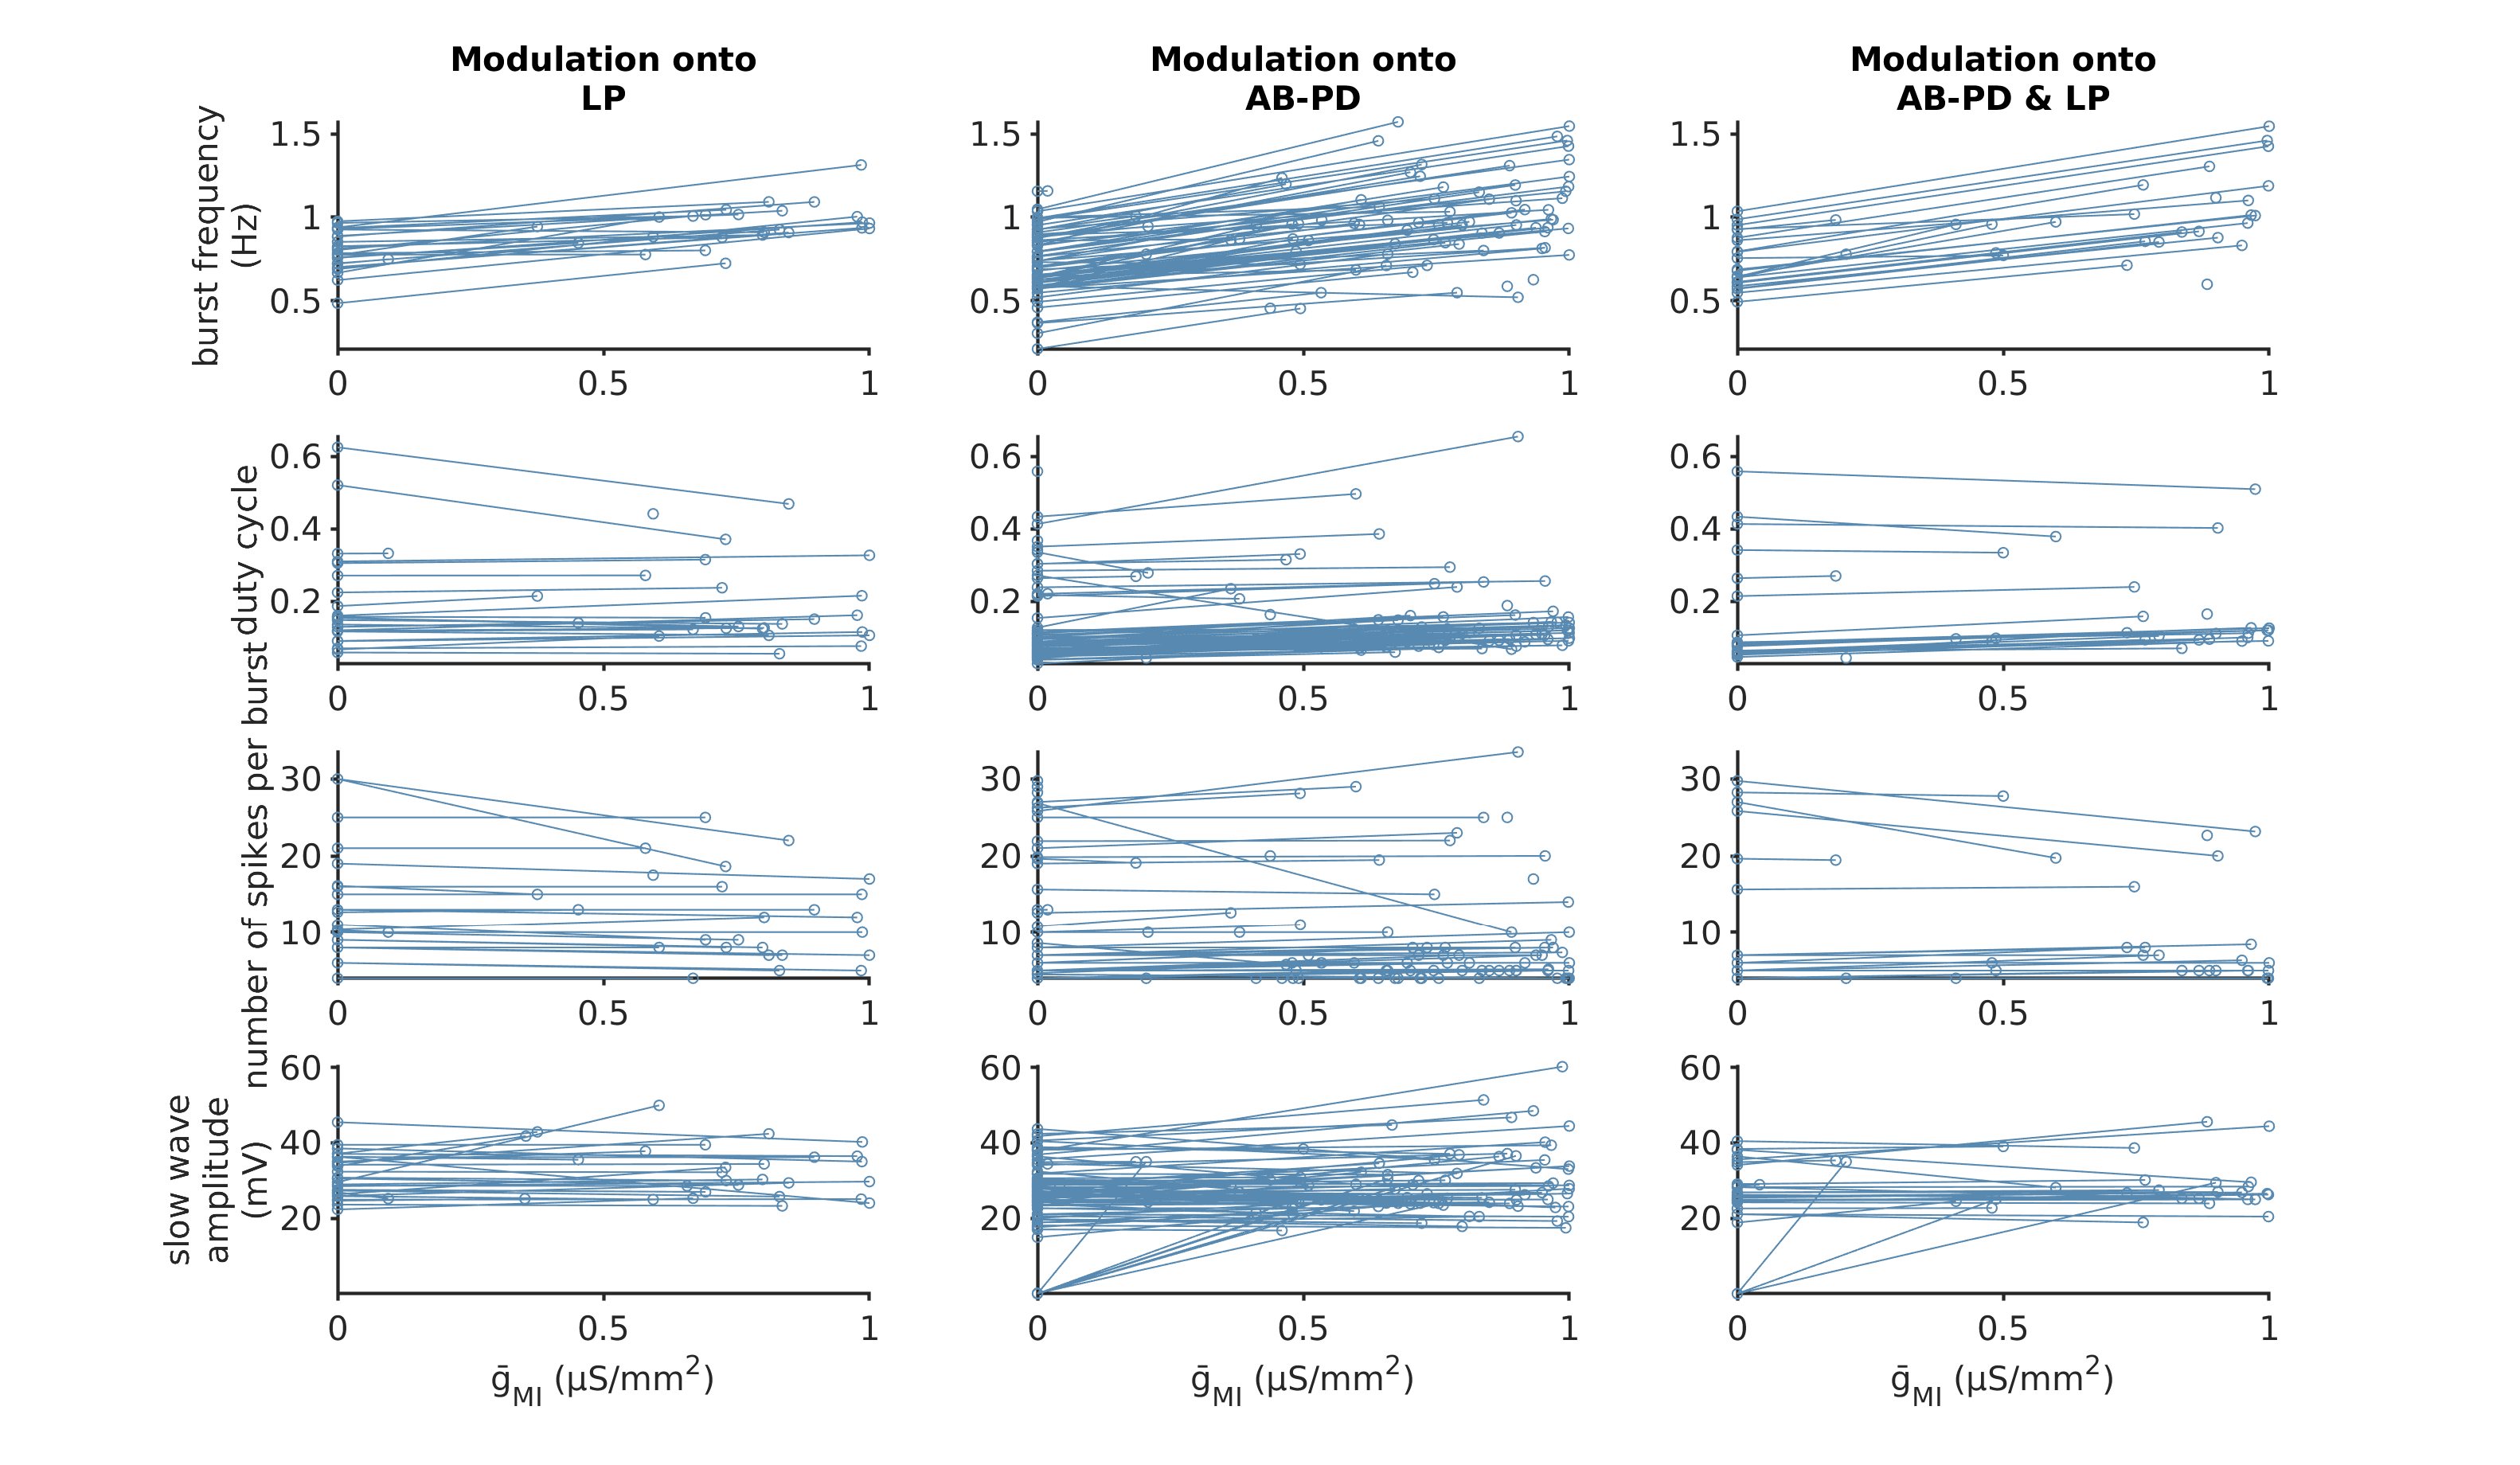
\includegraphics[width=1.0\linewidth]{gfx/all-modulation/metrics_AB}
	\caption[All optimized ABPD models in decentralized and modulated cases]{146 network models in decentralized and modulated cases show increased burst frequency and amplitude under modulated conditions with respect to decentralization. Modulation under \acs{AB}-\acs{PD} and \acs{LP} produces the most regular triphasic output. Colors indicate cells (blue is \acs{AB}-\acs{PD}).}
	\label{fig:metricsab}
\end{figure}

\begin{figure}
	\centering
	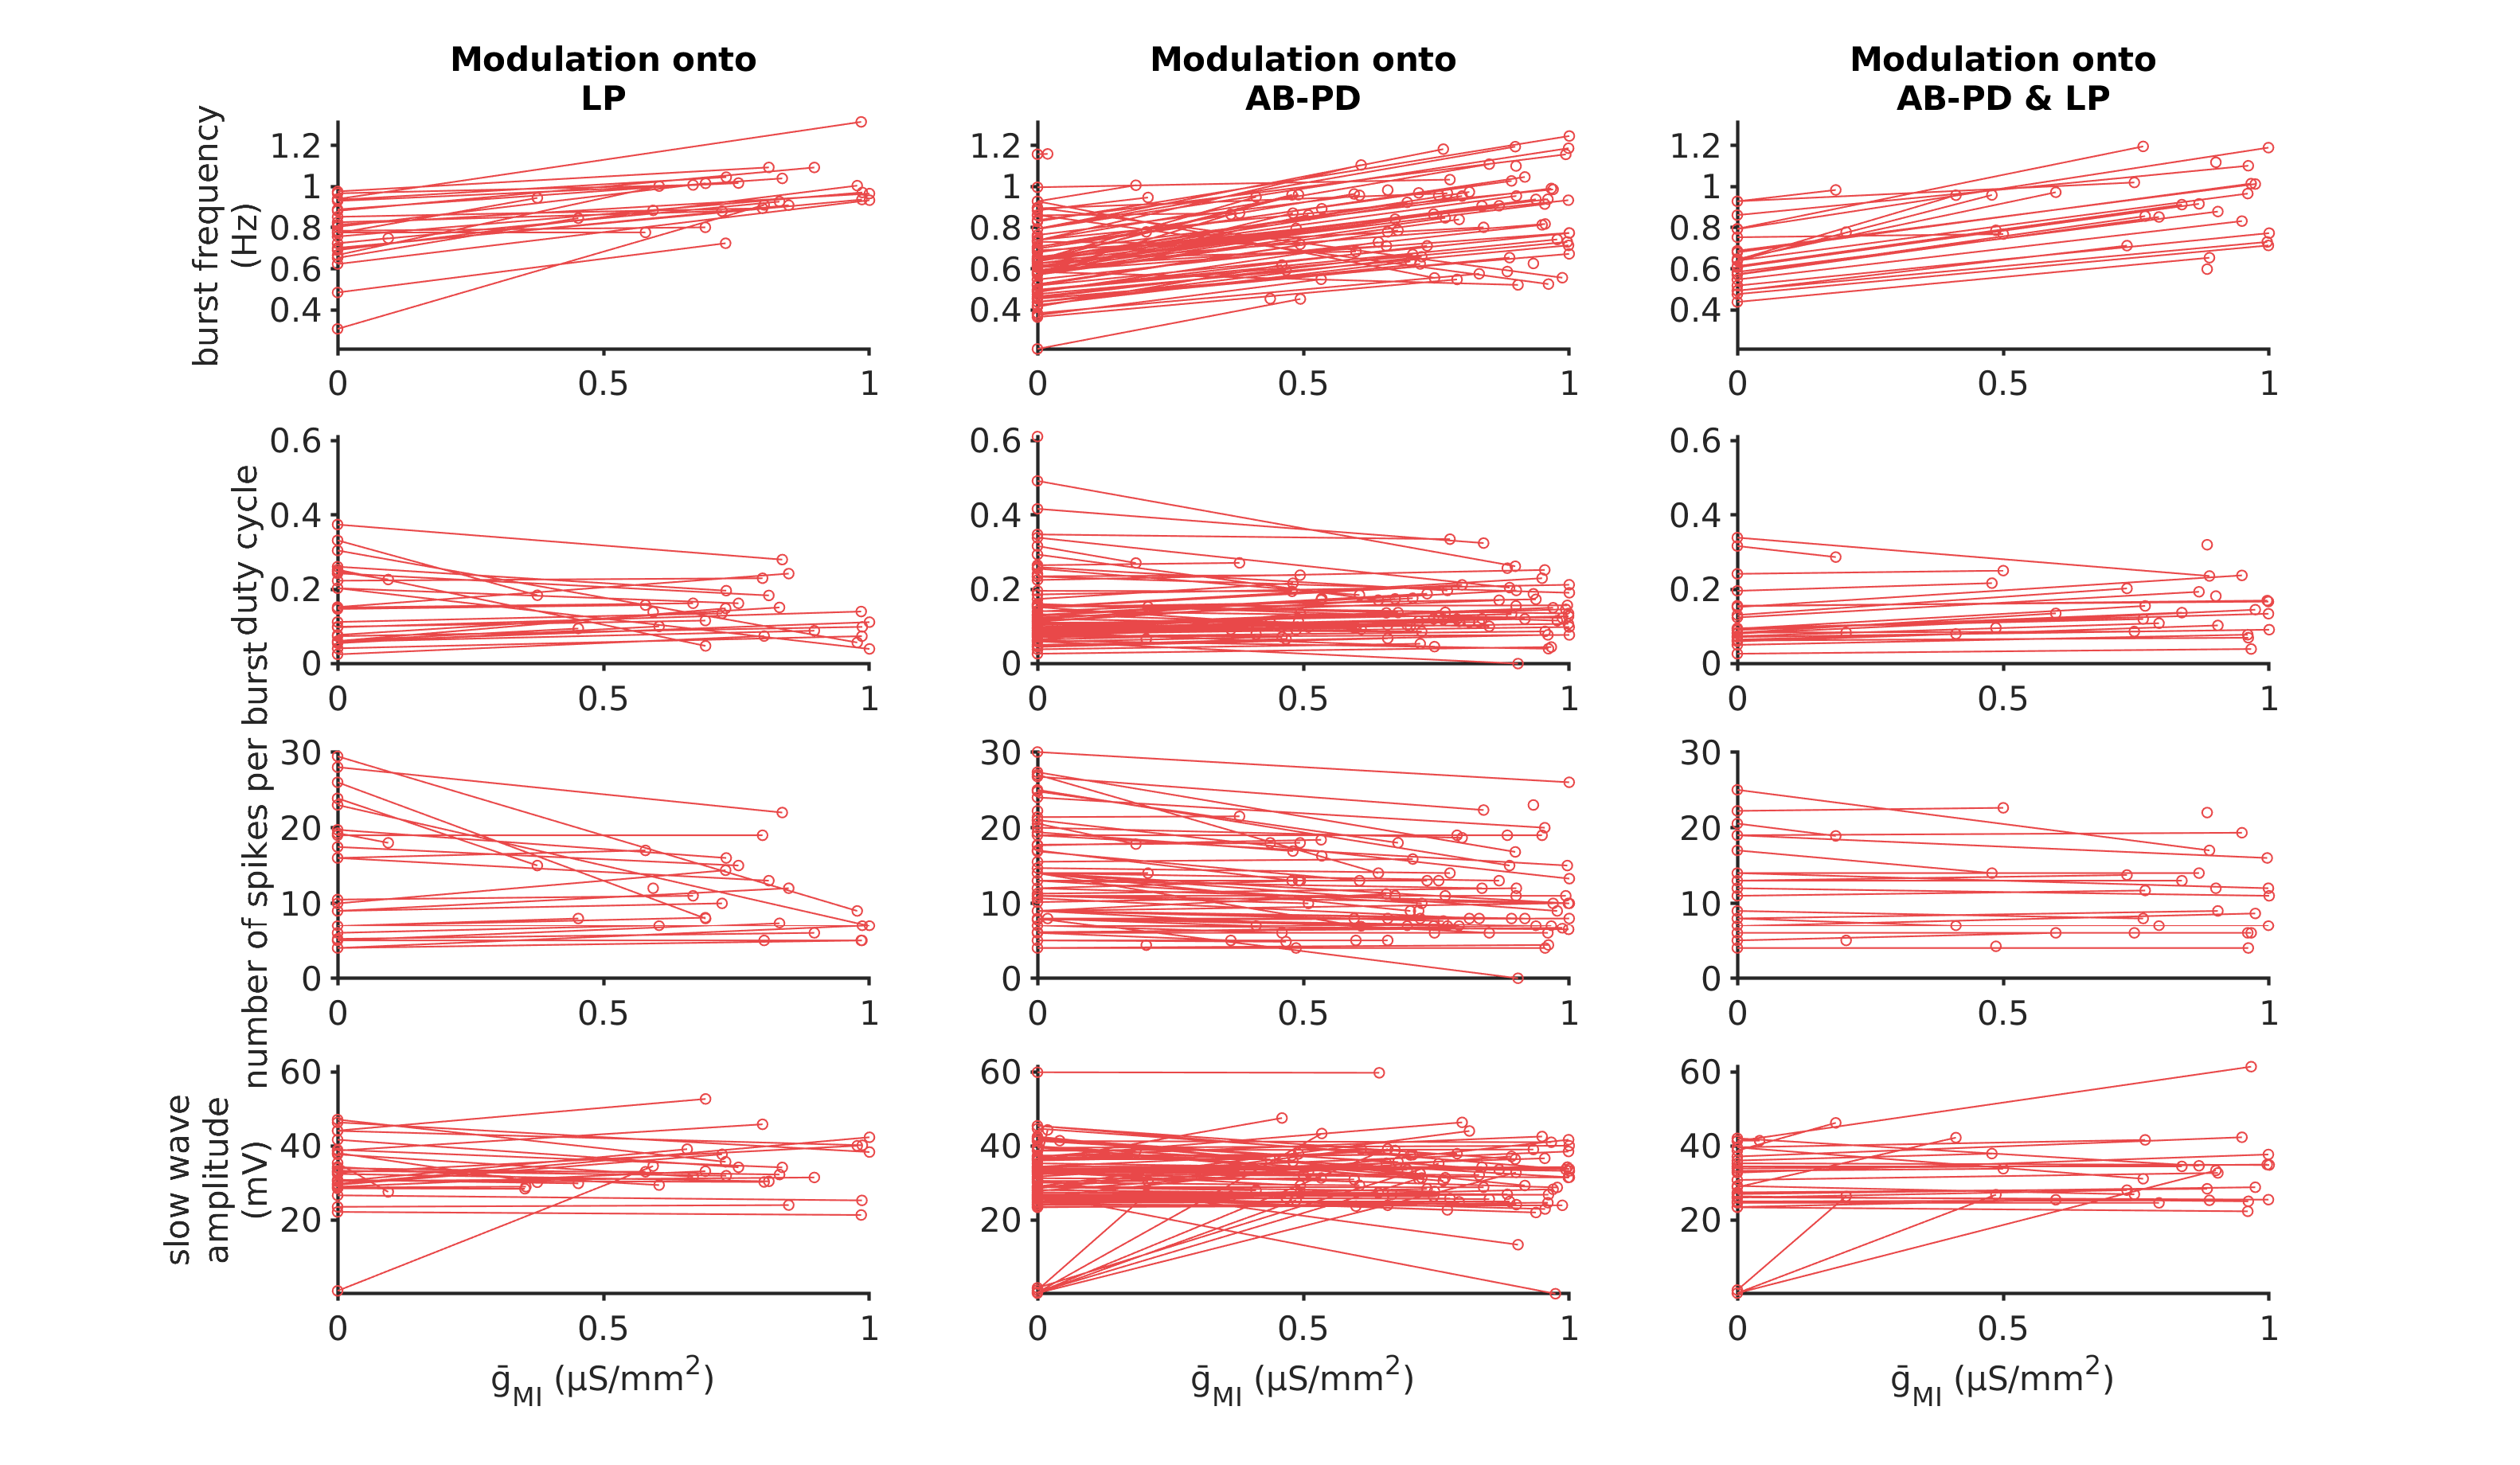
\includegraphics[width=1.0\linewidth]{gfx/all-modulation/metrics_LP}
	\caption[All optimized ABPD models in decentralized and modulated cases]{146 network models in decentralized and modulated cases show increased burst frequency and amplitude under modulated conditions with respect to decentralization. Modulation under \acs{AB}-\acs{PD} and \acs{LP} produces the most regular triphasic output. Colors indicate cells (red is \acs{LP}).}
	\label{fig:metricslp}
\end{figure}

\begin{figure}
	\centering
	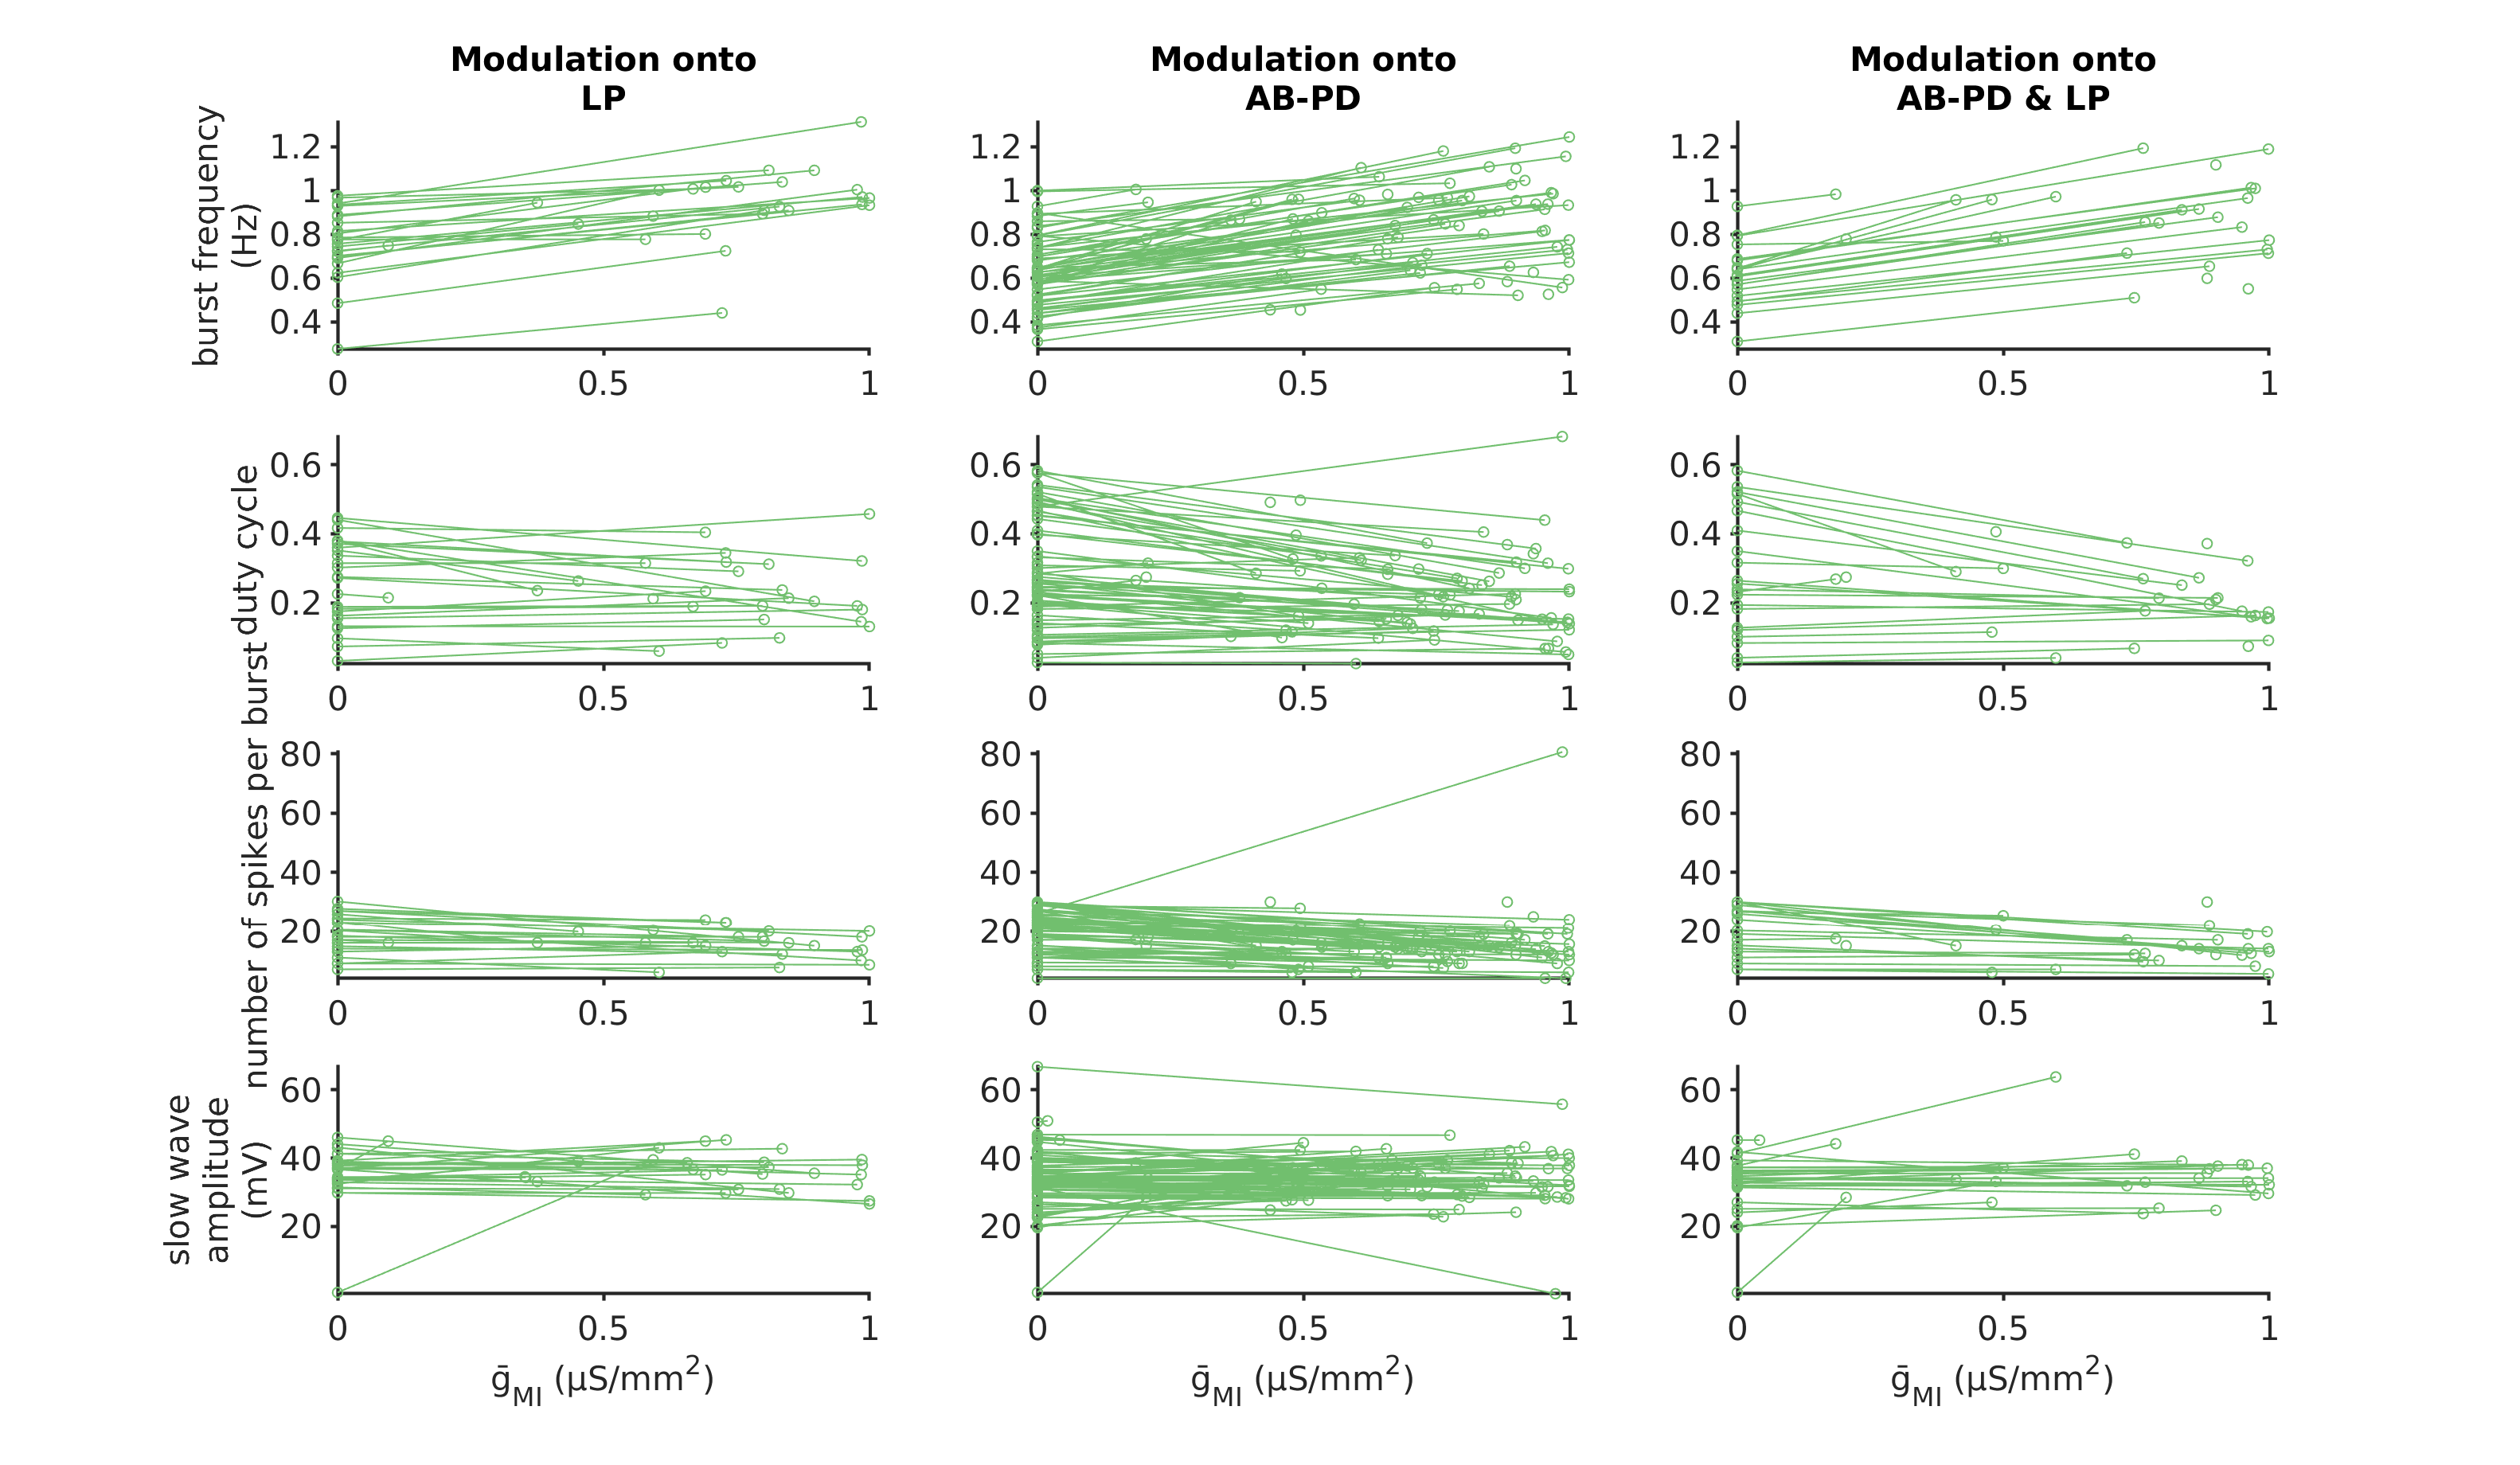
\includegraphics[width=1.0\linewidth]{gfx/all-modulation/metrics_PY}
	\caption[All optimized ABPD models in decentralized and modulated cases]{146 network models in decentralized and modulated cases show increased burst frequency and amplitude under modulated conditions with respect to decentralization. Modulation under \acs{AB}-\acs{PD} and \acs{LP} produces the most regular triphasic output. Colors indicate cells (green is \acs{PY}).}
	\label{fig:metricspy}
\end{figure}

\FloatBarrier

\subsection{Modulation of LP Can Inhibit AB-PD}

\autoref{fig:traces1} demonstrates a case where modulation onto \acs{LP} decreases \acs{AB}-\acs{PD} burst frequency, but modulation onto the pacemaker or \acs{AB}-\acs{PD} and \acs{LP} increases burst frequency. In \autoref{fig:metrics1}, the slow-wave amplitude and frequency of \acs{LP} increases, inhibiting the pacemaker, which bursts at a much slower frequency. If modulation is applied to \acs{AB}-\acs{PD} or the pacemaker kernel and \acs{LP}, the frequency increases. If the strength of the synapse is strong, pacemaker burst frequency decreases.

Applied current or \acs{IMI} tends to drive the rhythm, increasing burst frequency\autocite{DrionIonchanneldegeneracy2015,EisenMechanismsunderlyingpattern1982}. Modulation onto \acs{LP} inhibits the pacemaker, causing \acs{AB}-\acs{PD} to skip every other burst (\autoref{fig:traces2}). In both \autoref{fig:traces1} and \autoref{fig:traces2}, rhythmicity is maintained because synaptic transmission in the \acs{STG} is partially graded. Instead, if modulation is applied to the pacemaker kernel or the pacemaker kernel and \acs{LP}, the frequency increases by 60\% (\autoref{fig:traces2}). These models recapitulate the role of \acs{AB}-\acs{PD} as the pacemaker kernel in the pyloric circuit. 

Modulated neurons tend to maintain the same number of spikes per burst and duty cycle despite the higher frequency\autocite{EisenMechanismsunderlyingpattern1982,SwensenMultiplepeptidesconverge2000}. Those which are not modulated typically fall behind. This is likely due to the fact that modulation acts at the spike threshold but does not contribute significantly to the spiking waveform. Non-modulated cells experience increased inhibition in the same period of time; the membrane potential does not depolarize as much between bouts of inhibition, decreasing slow-wave amplitude.

\subsection{Modulation of AB Can Elicit Tonic Spiking}

In some cases in the model, modulation onto the pacemaker has deleterious effects on the rhythm. If \acs{AB}-\acs{PD} is depolarized by addition of inward current near the spiking threshold, rhythmicity is lost (\autoref{fig:traces3}); the neuron is close to a transition to a tonic spiking regime. If instead, \acs{LP} is modulated, increasing inhibition onto the pacemaker drives the frequency (\autoref{fig:metrics3}). Interestingly, in the case where \acs{IMI} activates in the pacemaker kernel and \acs{LP}, rhythmicity is maintained, and burst frequency and slow-wave amplitude increase.

This result is likely non-physiological. Injected current into \acs{AB} depolarizes the membrane, but generally does not elicit tonic spiking (\autoref{fig:sharp2})\autocite{SwensenModulatorsconvergentcellular2001,Soto-TrevinoComputationalmodelelectrically2005}. The pacemaker is also not readily susceptible loss of rhythmicity from hyperpolarization due to a constant current\autocite{Soto-TrevinoComputationalmodelelectrically2005}. The modulatory input recorded in \citeauthor{SwensenModulatorsconvergentcellular2001}\autocite{SwensenModulatorsconvergentcellular2001} cannot produce the sustained excitatory or inhibitory pulses of current necessary to cease endogenous bursting. In light of this, modulation onto \acs{LP} contributes less to the increase in burst frequency and amplitude seen with proctolin and \acs{RPCH}. 

Given that most \acs{AB}-\acs{PD} pacemakers must be far from transitions into depolarization block and tonic spiking regimes and be robust to hyperpolarization\autocite{WeimannModulationOscillatorInteractions1997,Harris-WarrickDynamicBiologicalNetworks1992}, the models suggest that modulation of \acs{LP} likely serves an ancillary role in in initiation and maintenance of robust triphasic motor patterns. These conclusions are supported by experiments with \ac{CCAP}, in which modulation of \acs{LP} while the pacemaker was hyperpolarized was insufficient to initiate the pyloric rhythm\autocite{WeimannModulationOscillatorInteractions1997}.

\FloatBarrier

\begin{figure}[t]
	\centering
	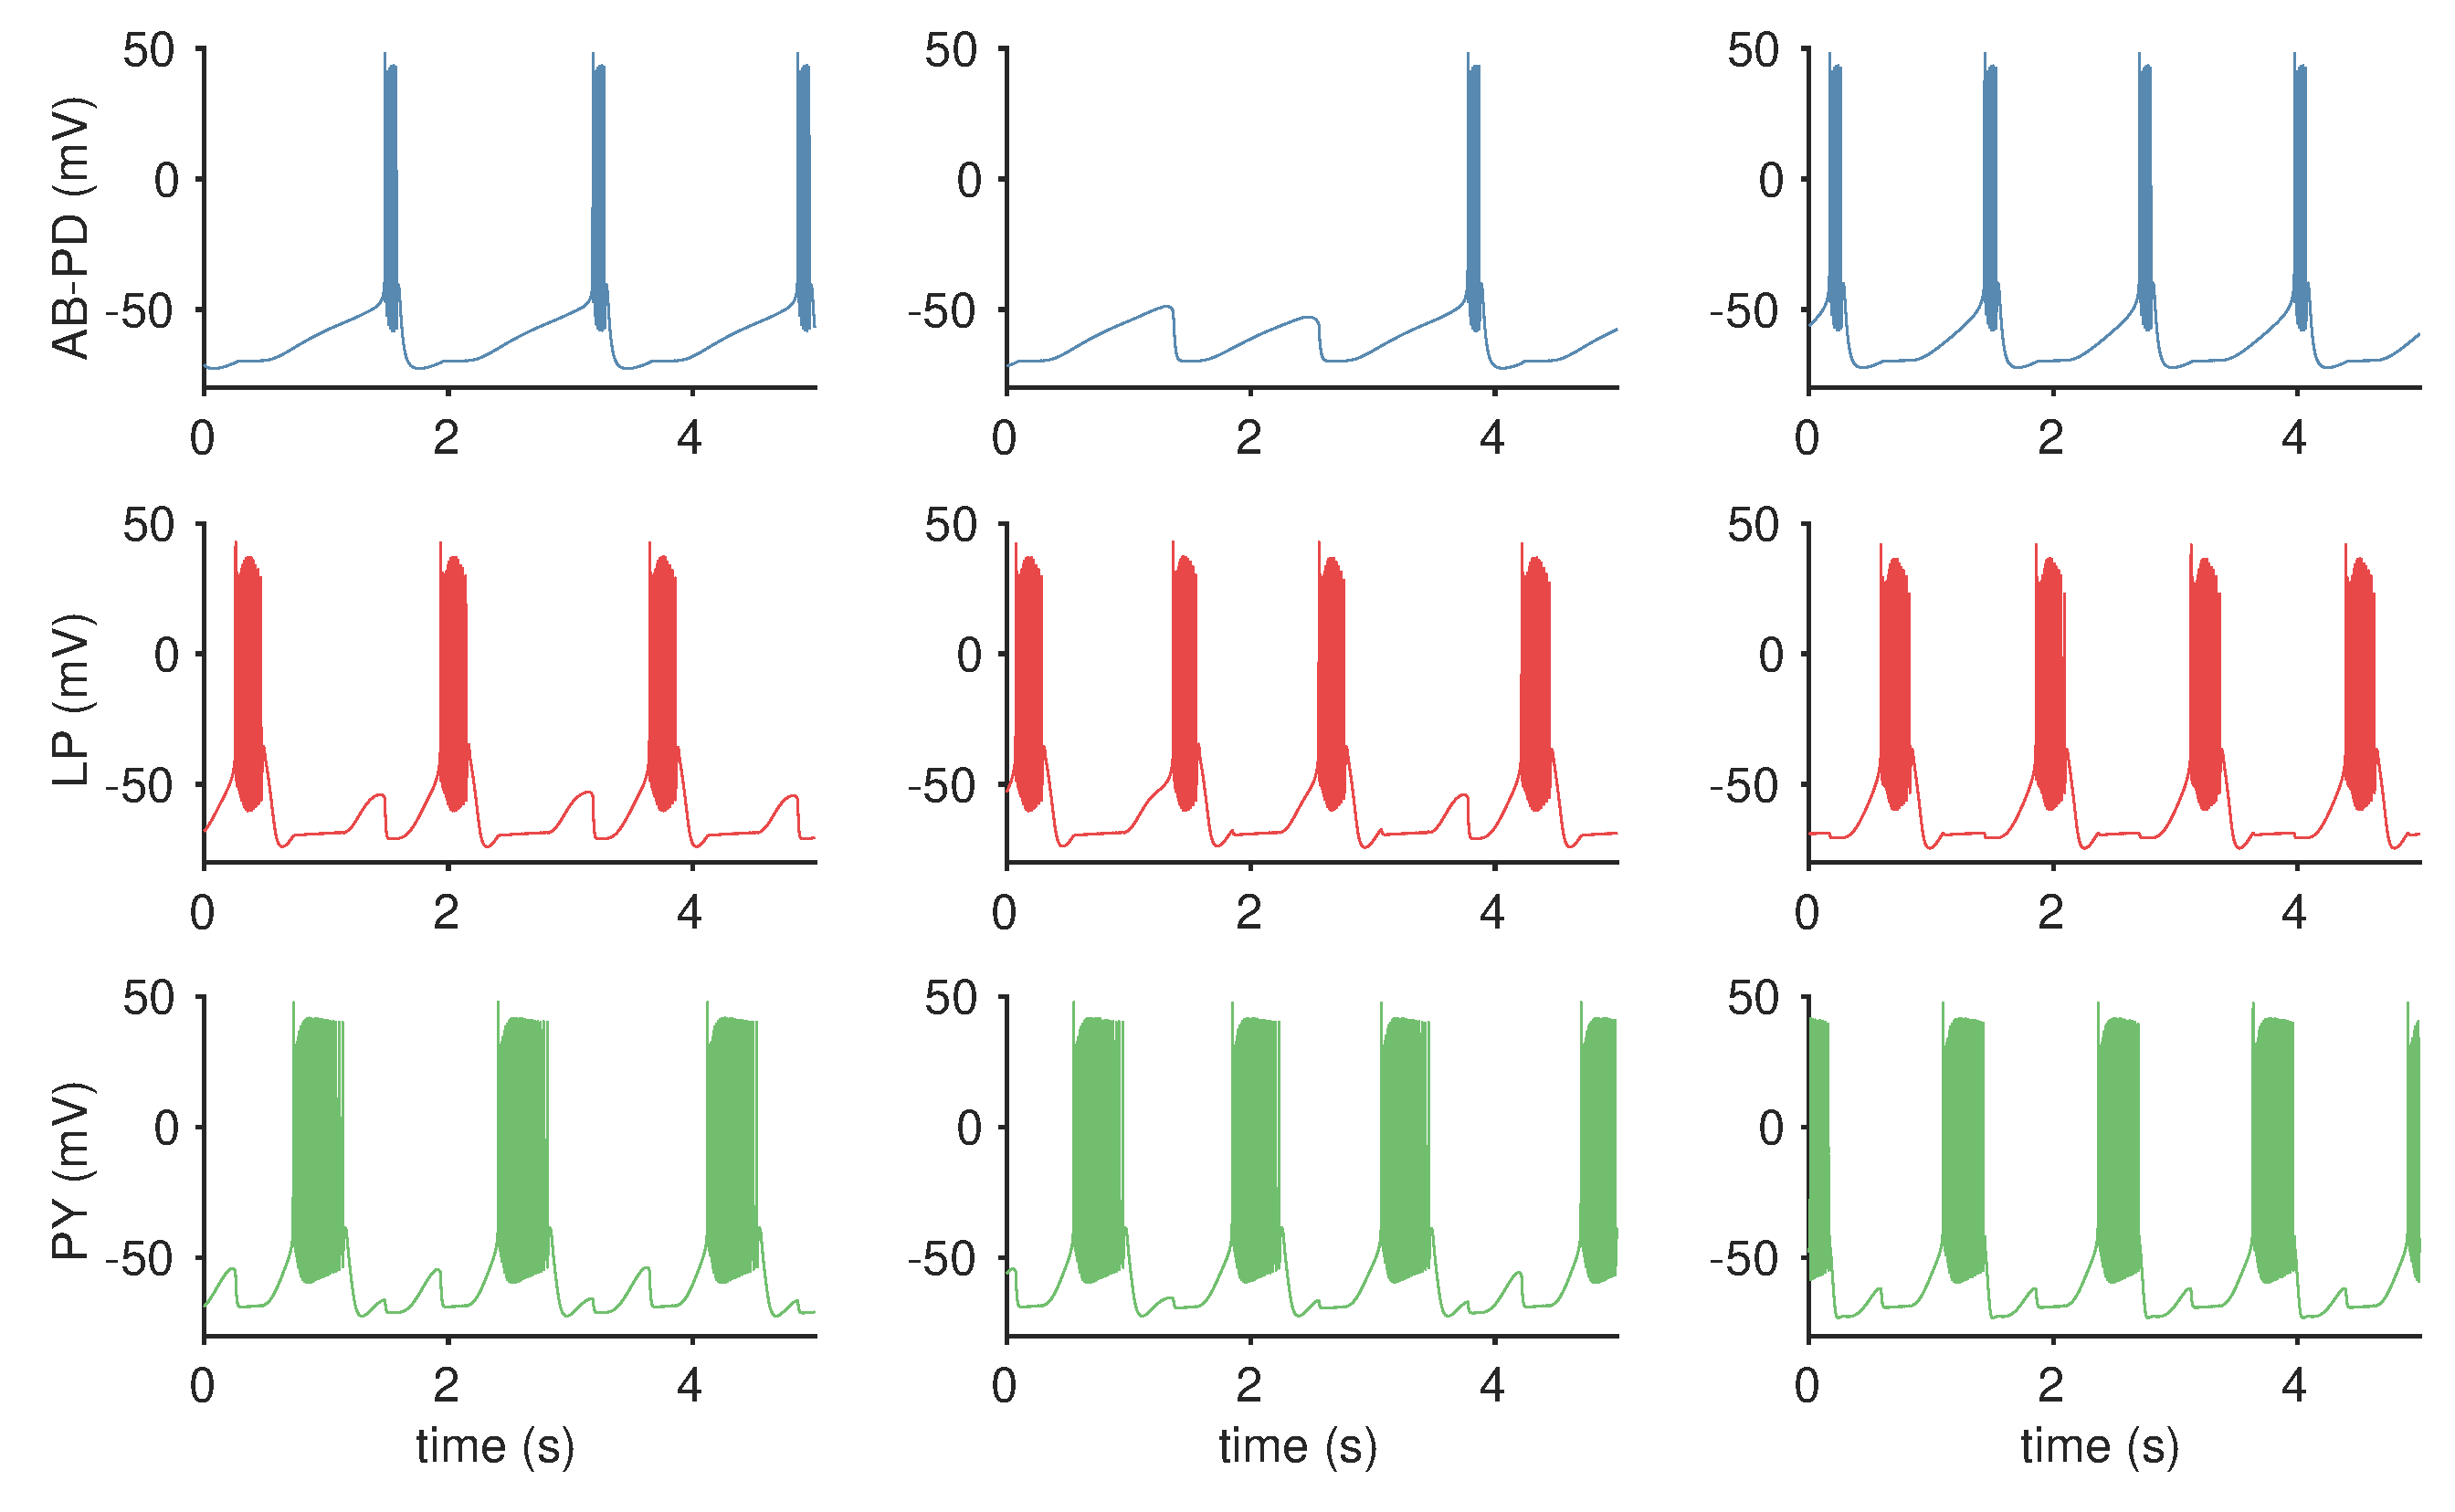
\includegraphics[width=1.0\linewidth]{gfx/all-modulation/traces1}
	\caption[Modulation onto LP inhibits the pacemaker (traces)]{Neuromodulation onto \acs{LP} can inhibit the pacemaker. Cells in columns are in the same network. \textit{Left:} No neuromodulation and a normal triphasic rhythm. \textit{Middle:} $\bar{g}_{MI}^{LP} = 0.2~\mu \mathrm{S/mm^2}$, the pacemaker is inhibited by \acs{LP}. \textit{Right:} Recovery, where $\bar{g}_{MI}^{LP} = \bar{g}_{MI}^{AB-PD} = 0.6~\mu \mathrm{S/mm^2}$, normal triphasic rhythm with increased frequency.}
	\label{fig:traces1}
\end{figure}

\begin{figure}[b]
	\centering
	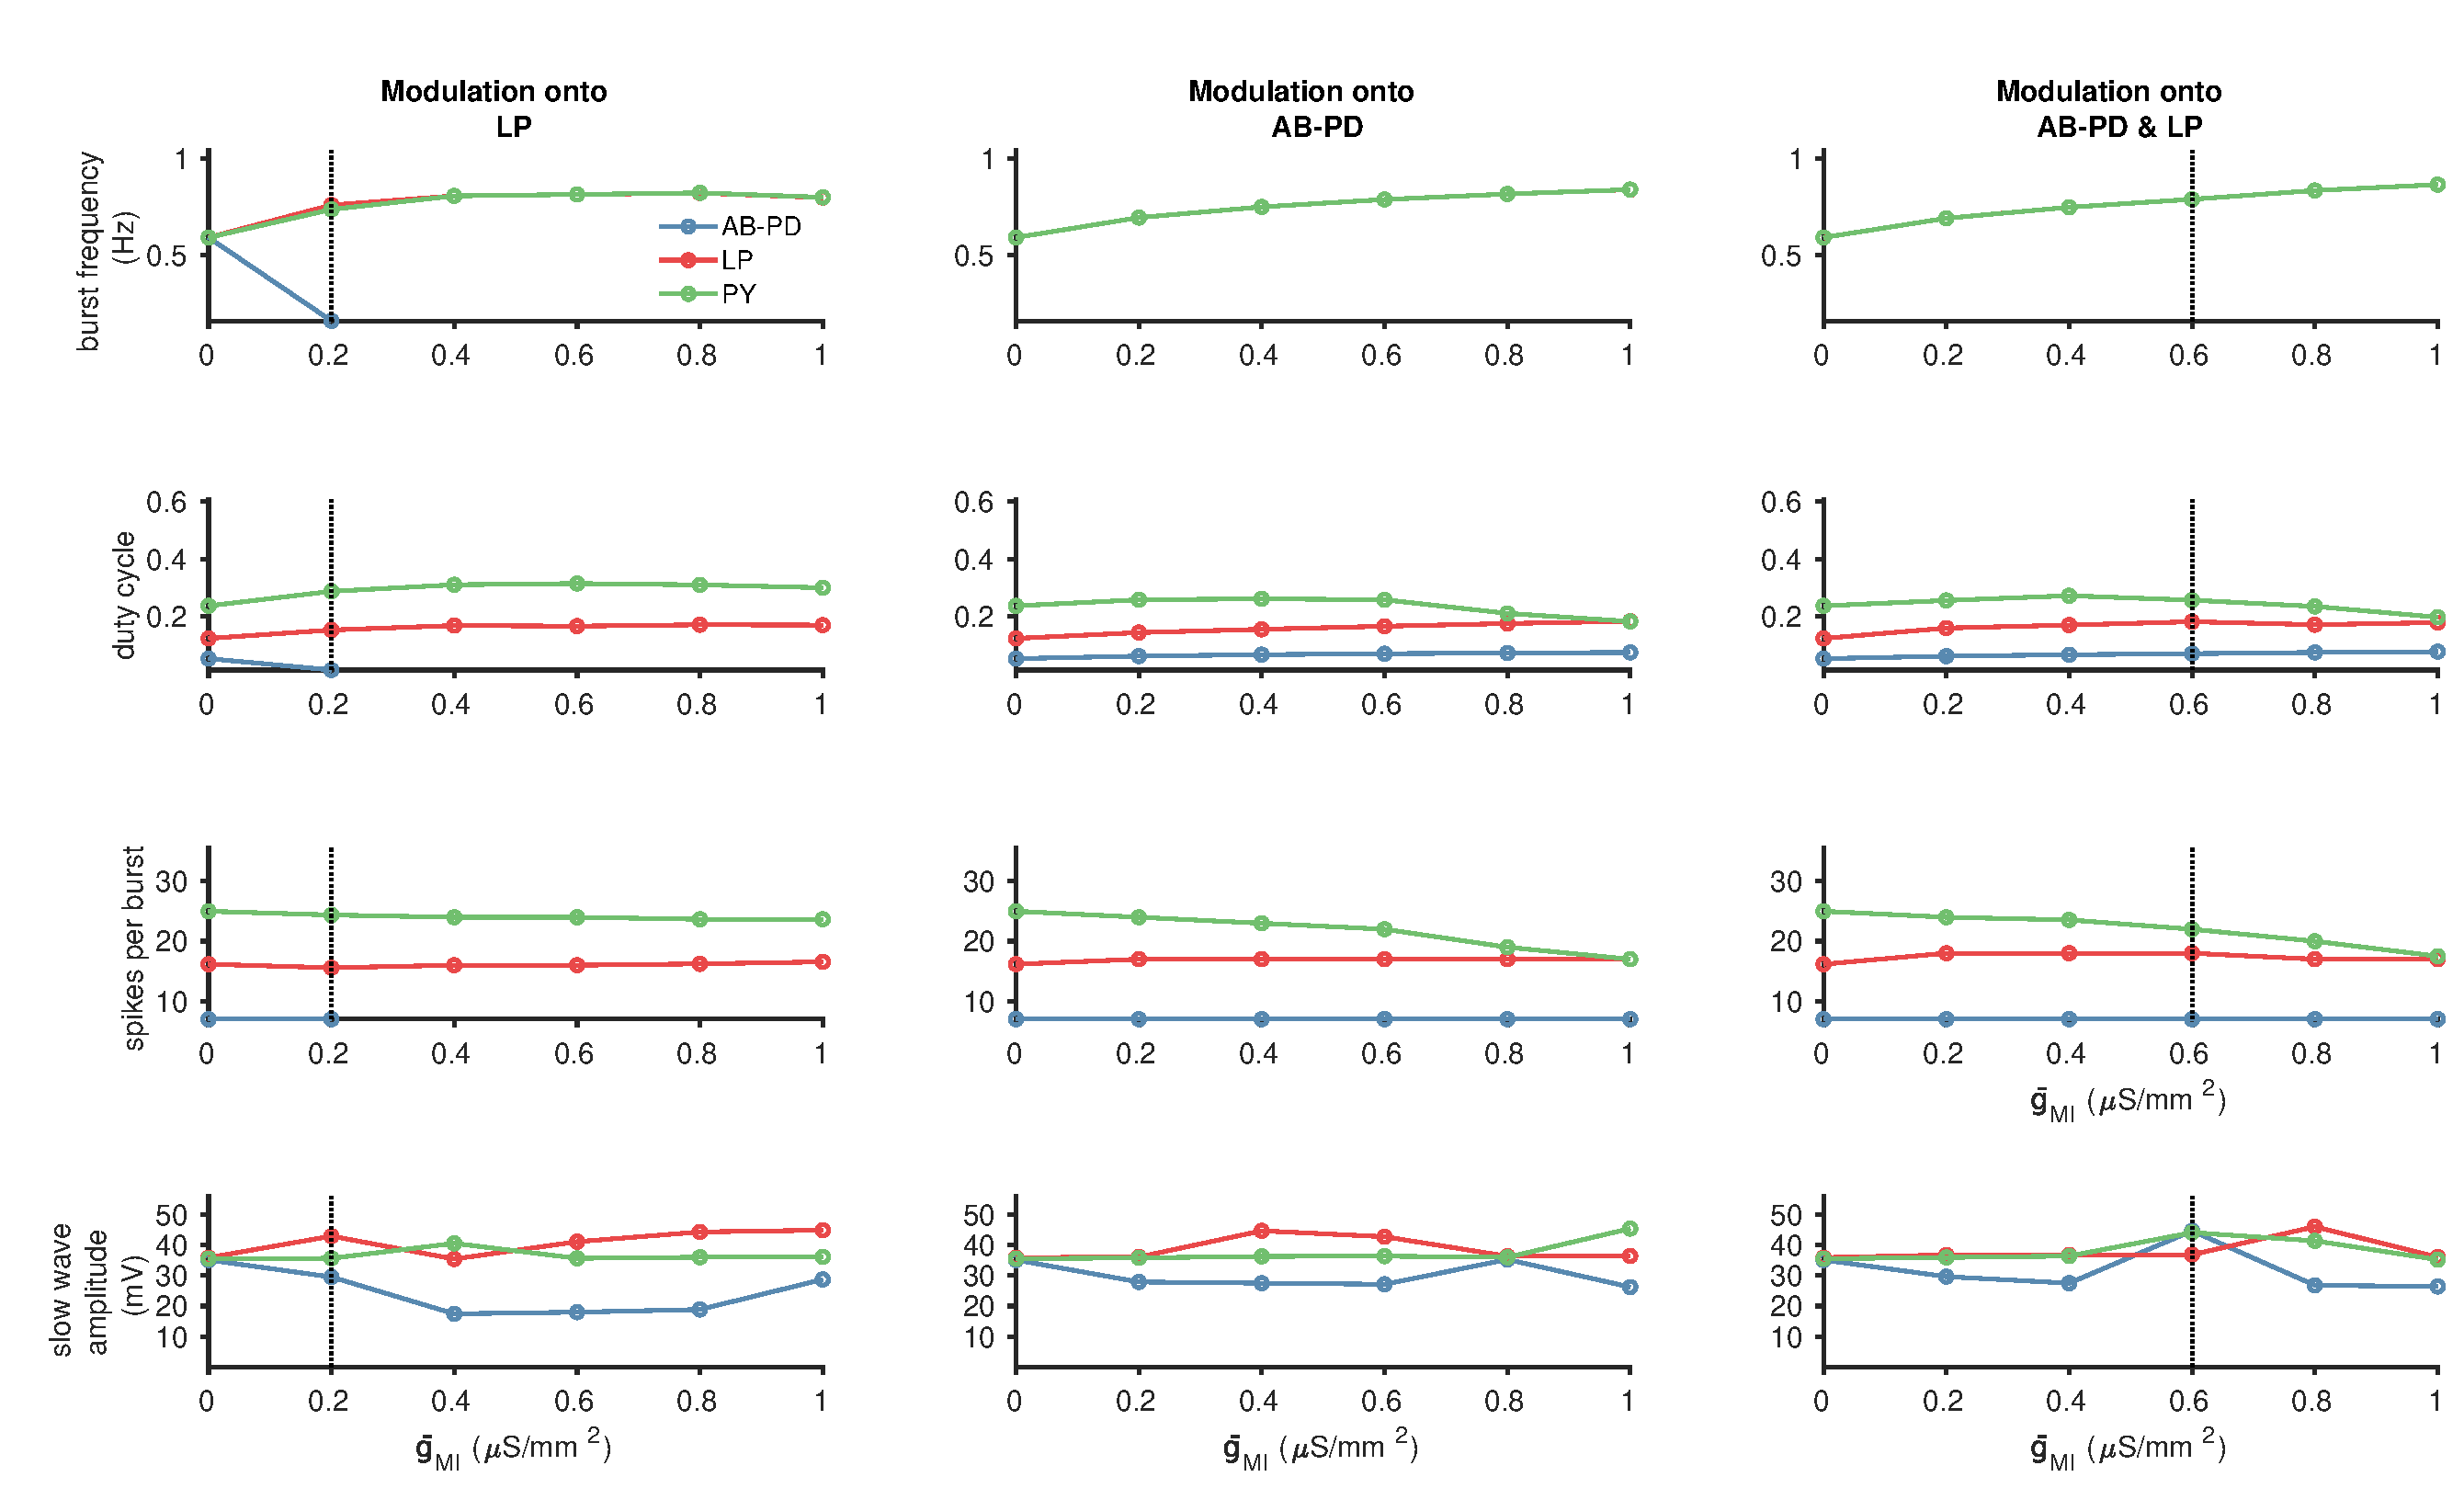
\includegraphics[width=1.0\linewidth]{gfx/all-modulation/metrics1}
	\caption[Modulation onto LP inhibits the pacemaker (metrics)]{Neuromodulation onto \acs{LP} can inhibit the pacemaker. Columns display metrics calculated at steady-state for three cases of modulation. Colors indicate cells (blue is \acs{AB}-\acs{PD}, red is \acs{LP}, green is \acs{PY}). Voltage traces at the dotted lines are shown in \autoref{fig:traces1}.}
	\label{fig:metrics1}
\end{figure}

\FloatBarrier

\begin{figure}[t]
	\centering
	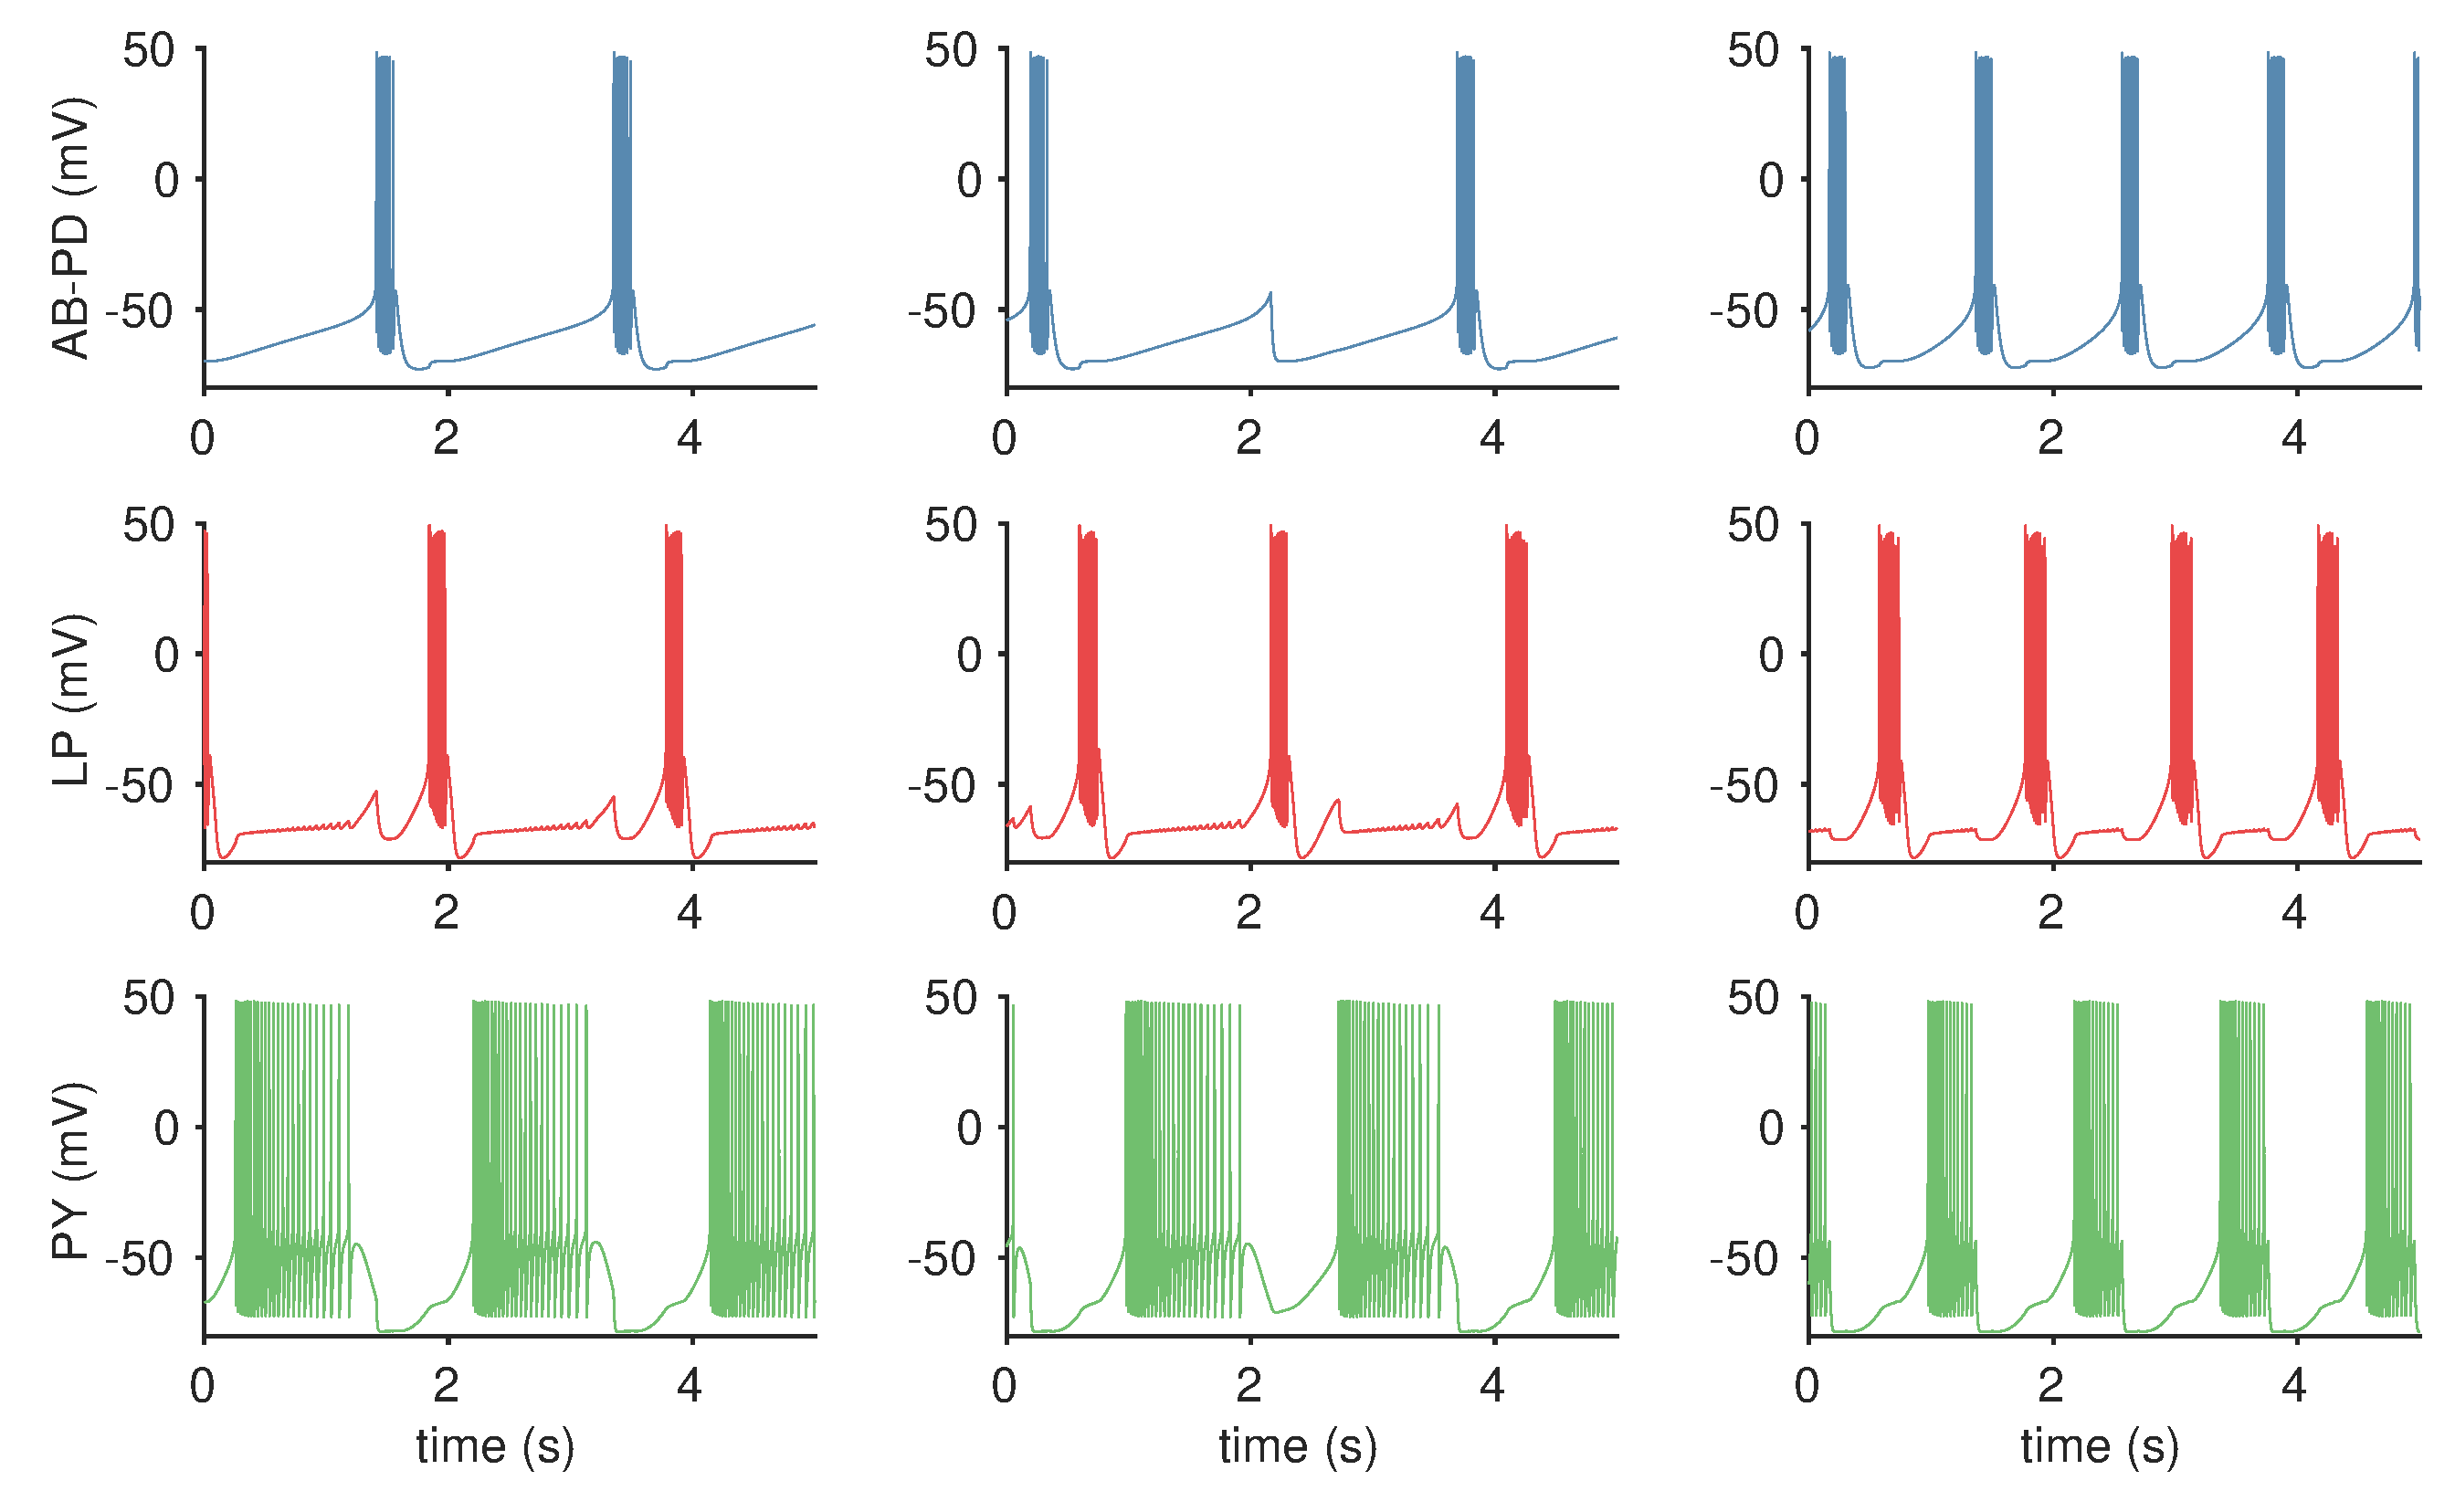
\includegraphics[width=1.0\linewidth]{gfx/all-modulation/traces2}
	\caption[Modulation onto LP does not increase frequency (traces)]{Neuromodulation onto \acs{LP} does not increase burst frequency. Cells in columns are in the same network. \textit{Left:} No neuromodulation and a normal triphasic rhythm. \textit{Middle:} $\bar{g}_{MI}^{LP} = 0.8~\mu \mathrm{S/mm^2}$, \acs{LP} inhibits \acs{AB}-\acs{PD}. \textit{Right:} Recovery, where $\bar{g}_{MI}^{LP} = \bar{g}_{MI}^{AB-PD} = 1.0~\mu \mathrm{S/mm^2}$, normal triphasic rhythm with increased frequency.}
	\label{fig:traces2}
\end{figure}

\begin{figure}[b]
	\centering
	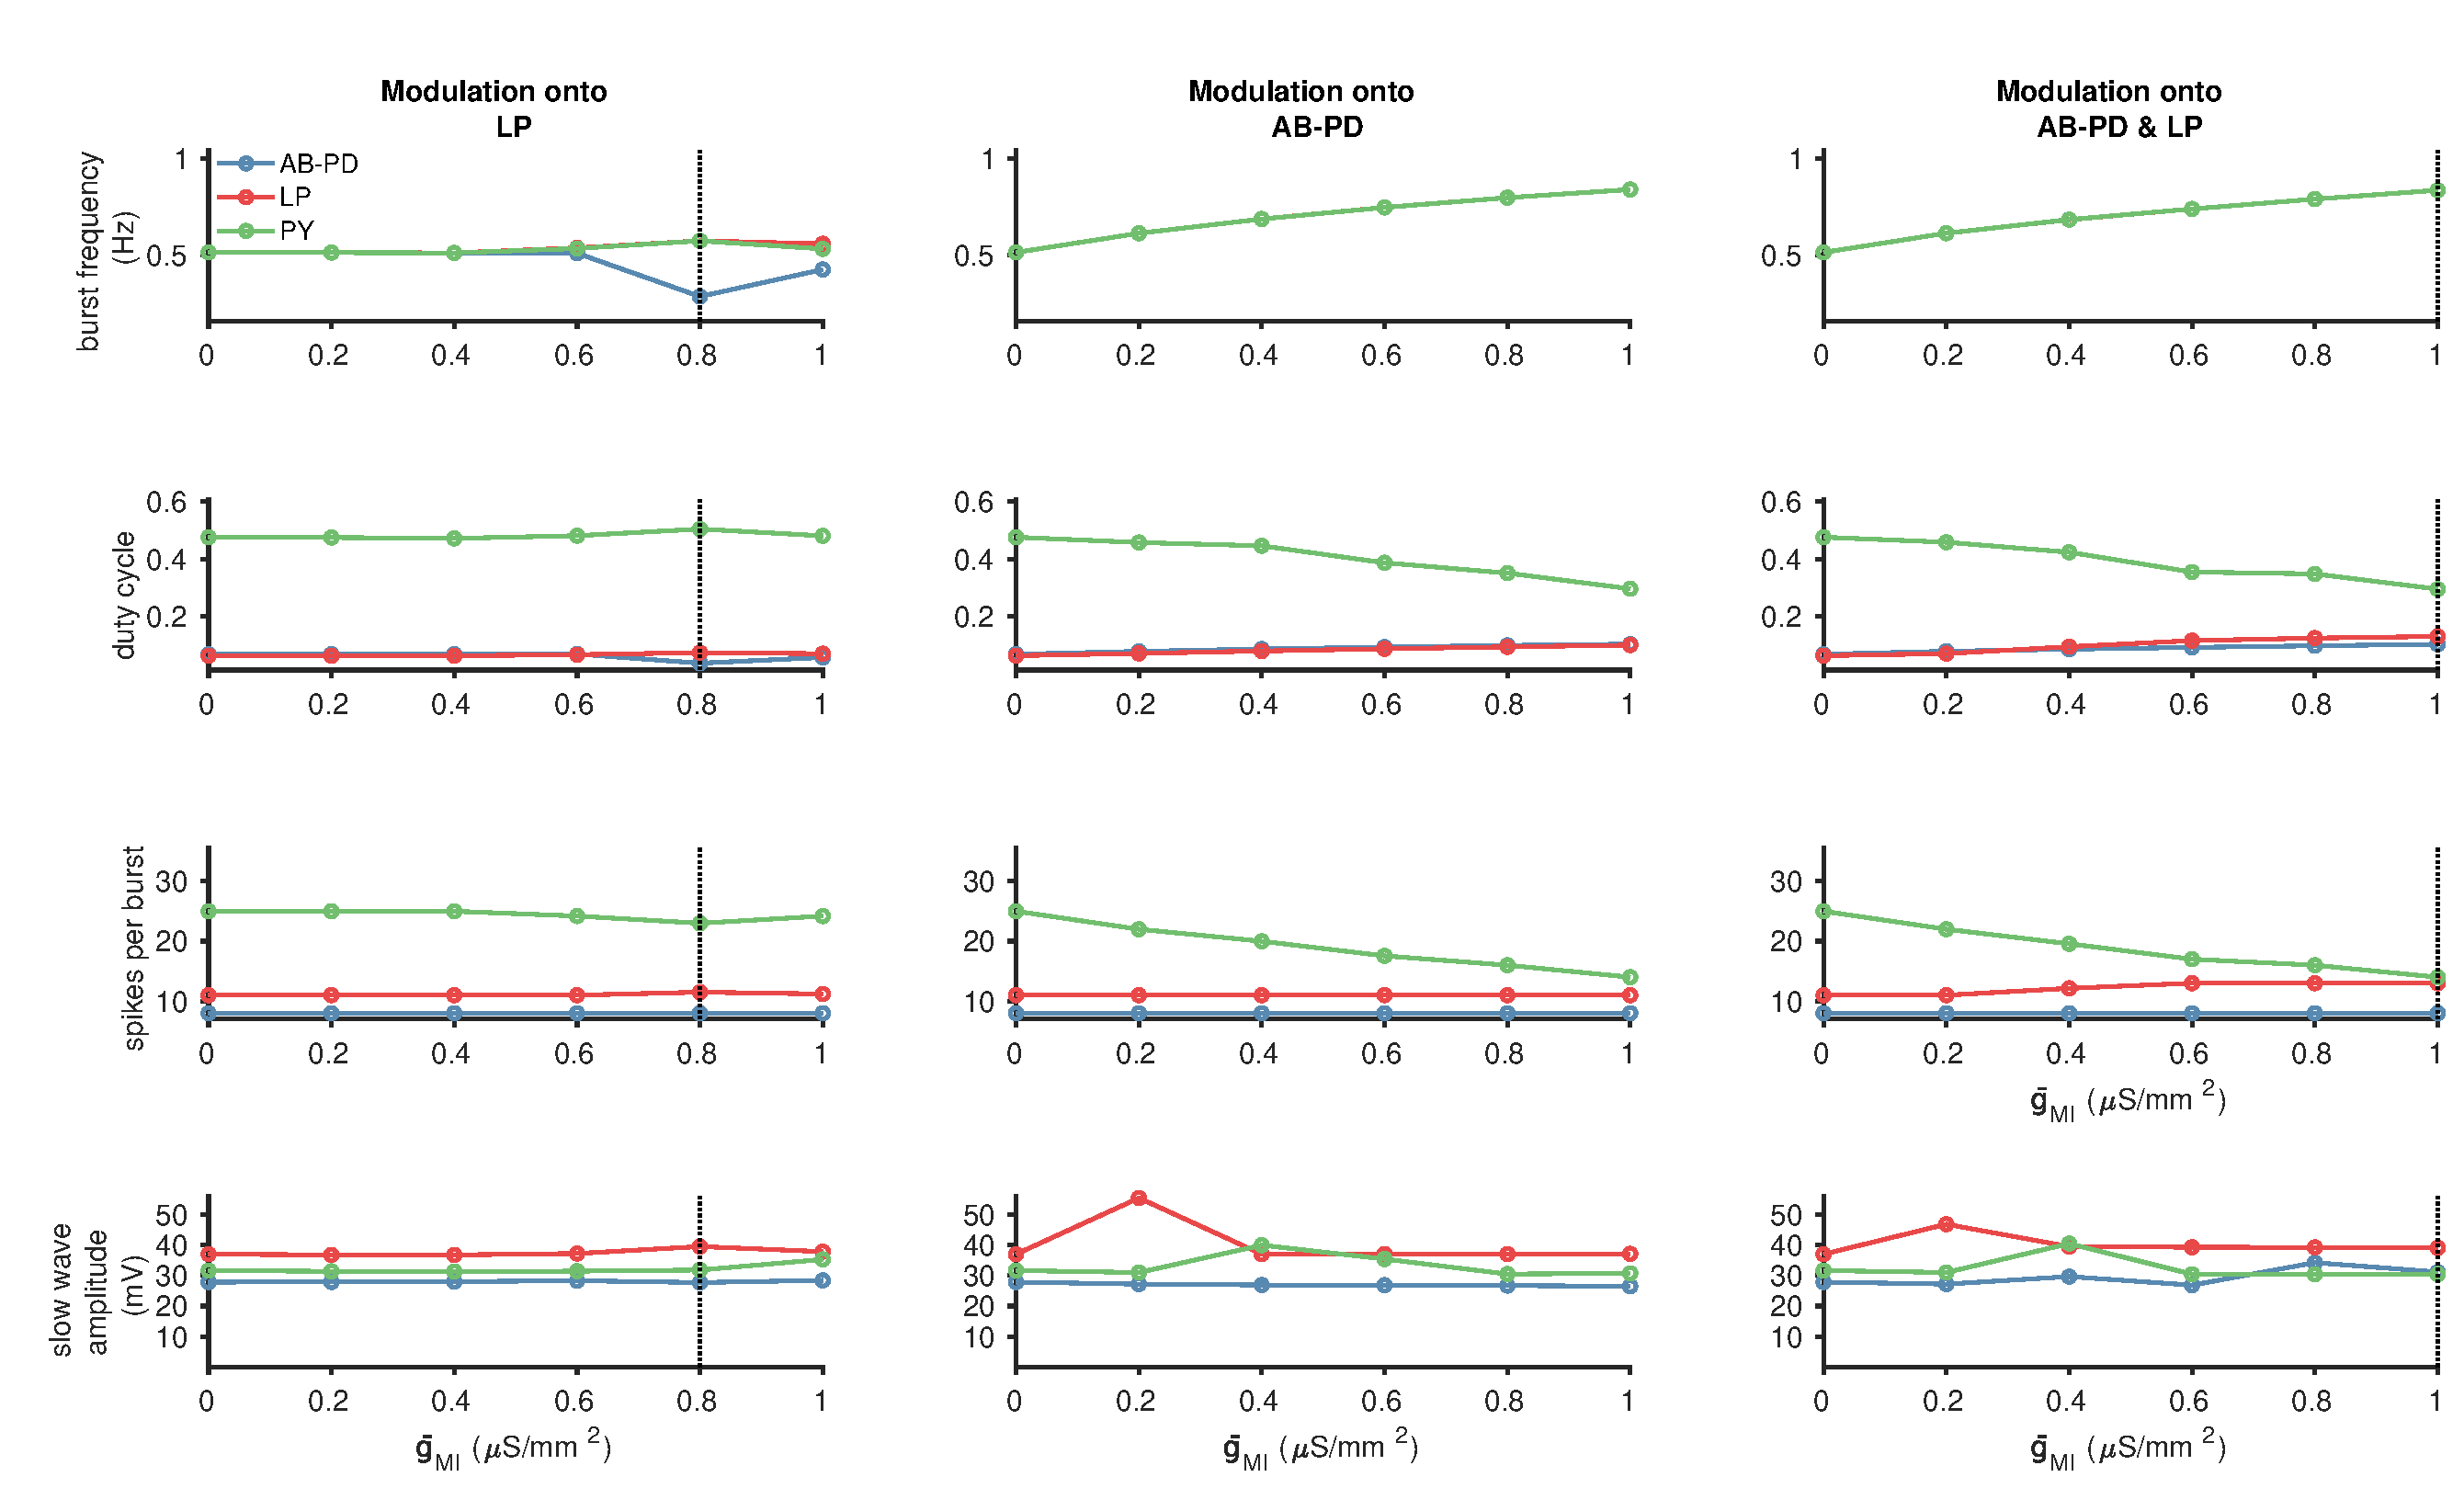
\includegraphics[width=1.0\linewidth]{gfx/all-modulation/metrics2}
	\caption[Modulation onto LP does not increase frequency (metrics)]{Neuromodulation onto \acs{LP} does not increase burst frequency in many models. Columns display metrics calculated at steady-state for three cases of modulation. Colors indicate cells (blue is \acs{AB}-\acs{PD}, red is \acs{LP}, green is \acs{PY}). Voltage traces at the dotted lines are shown in \autoref{fig:traces2}.}
	\label{fig:metrics2}
\end{figure}

\FloatBarrier

\begin{figure}[t]
	\centering
	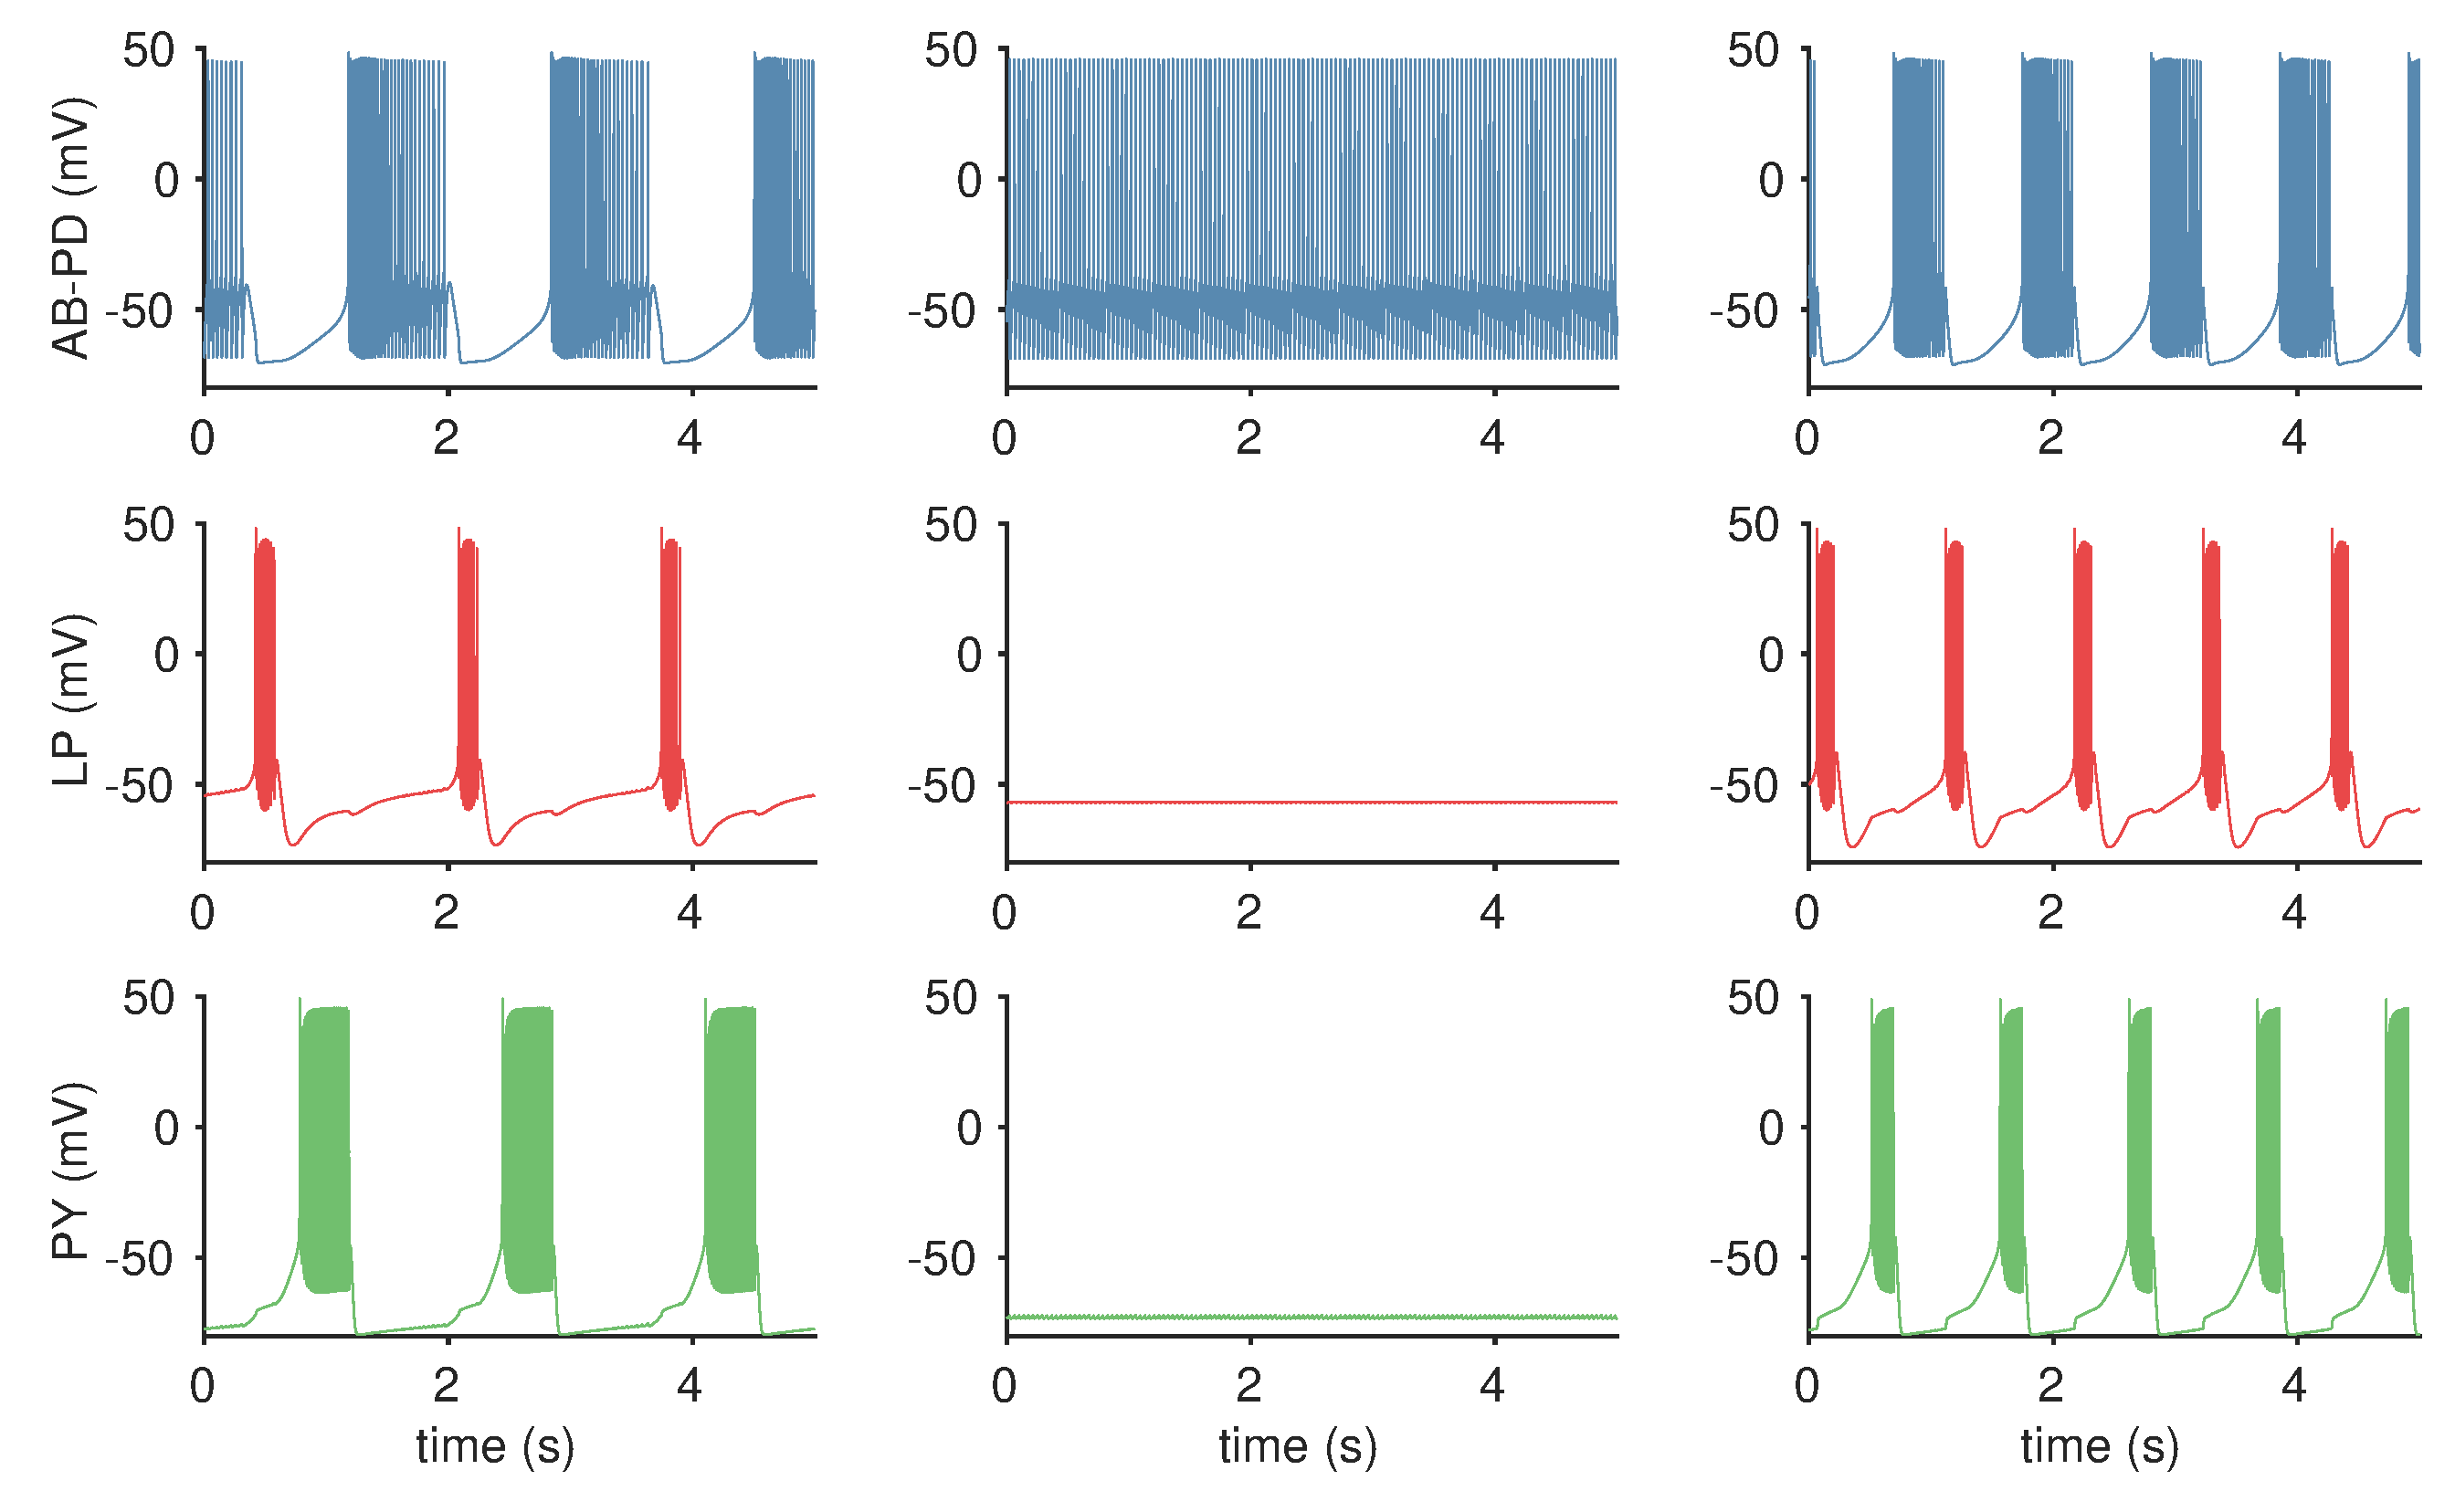
\includegraphics[width=1.0\linewidth]{gfx/all-modulation/traces3}
	\caption[Modulation of AB-PD depolarizes AB-PD (traces)]{Neuromodulation onto \acs{AB}-\acs{PD} can depolarize \acs{AB}-\acs{PD}. Cells in columns are in the same network. \textit{Left:} No neuromodulation and a normal triphasic rhythm. \textit{Middle:} $\bar{g}_{MI}^{AB-PD} = 0.6~\mu \mathrm{S/mm^2}$, \acs{AB}-\acs{PD} is tonically spiking. \textit{Right:} Normal triphasic rhythm, where $\bar{g}_{MI}^{LP} = \bar{g}_{MI}^{AB-PD} = 1.0~\mu \mathrm{S/mm^2}$, normal triphasic rhythm with increased frequency.}
	\label{fig:traces3}
\end{figure}

\begin{figure}[b]
	\centering
	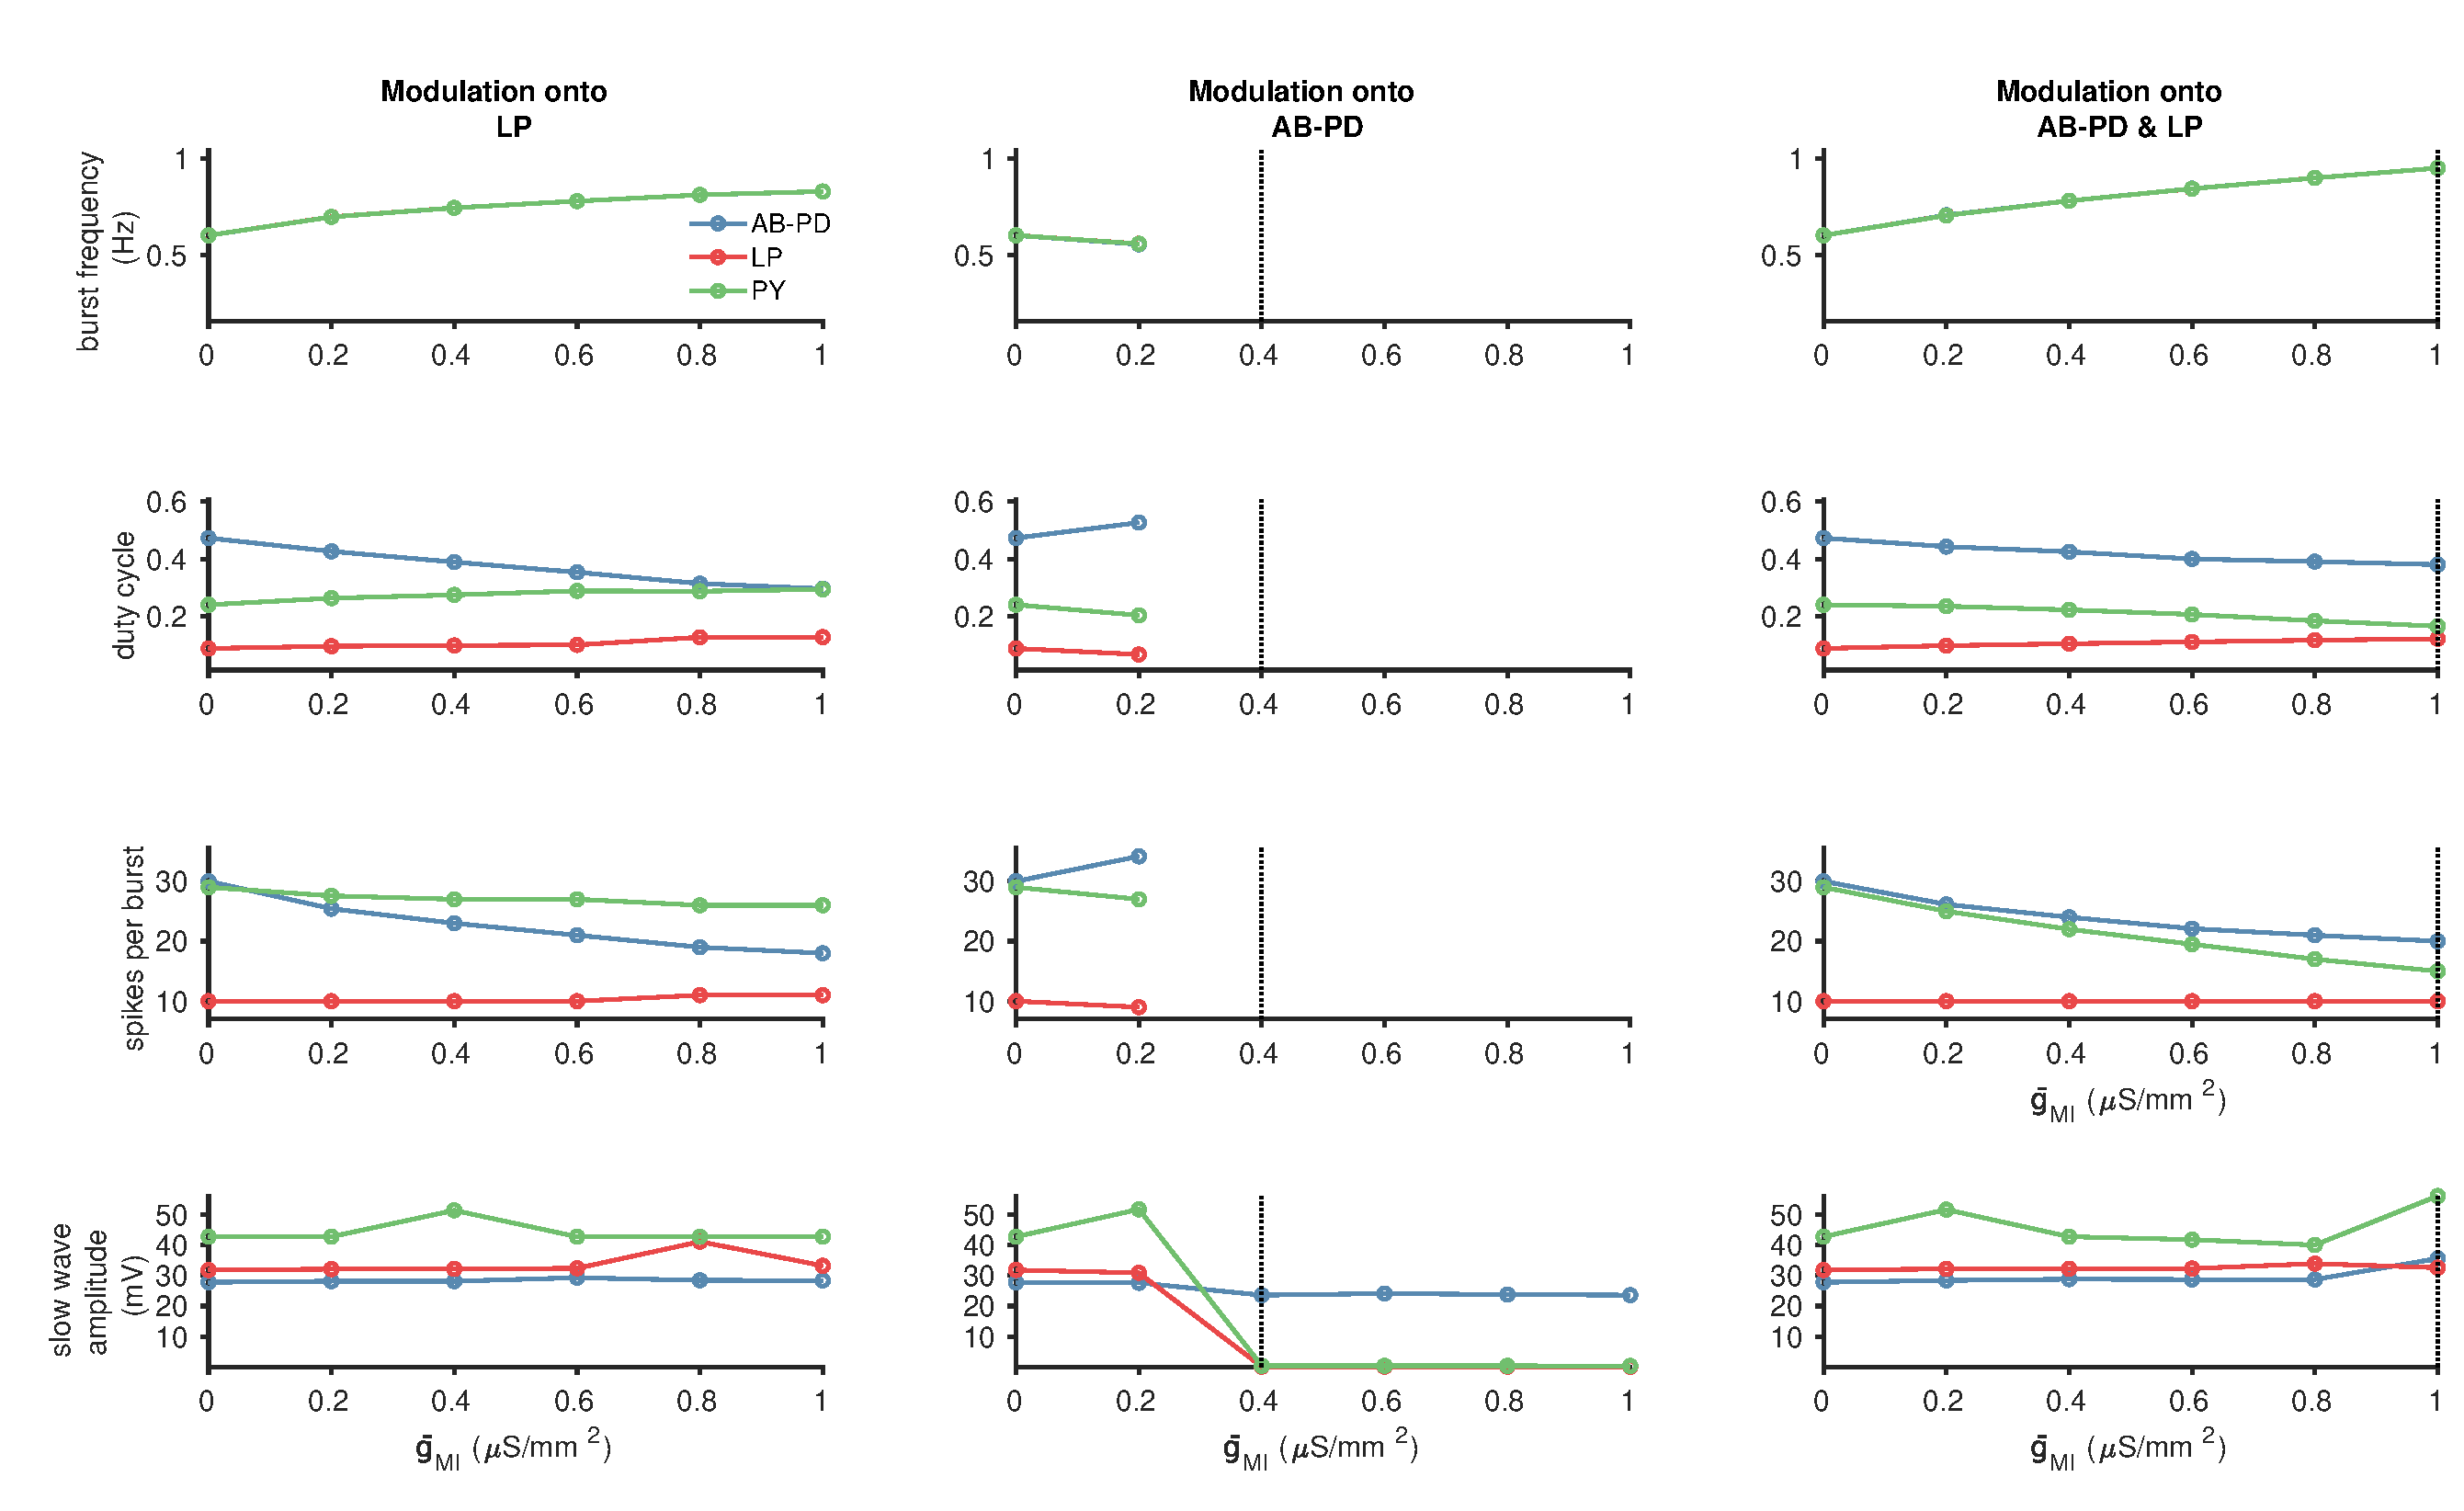
\includegraphics[width=1.0\linewidth]{gfx/all-modulation/metrics3}
	\caption[Modulation of AB-PD depolarizes AB-PD (metrics)]{Modulation onto \acs{AB}-\acs{PD} can depolarize the pacemaker, resulting in tonic spiking. Modulation of \acs{LP} or \acs{AB}-\acs{PD} and \acs{LP} results in normal triphasic rhythm with increasing burst frequency. Voltage traces at the dotted lines are shown in \autoref{fig:traces3}.}
	\label{fig:metrics3}
\end{figure}

\FloatBarrier

\begin{figure}[t]
	\centering
	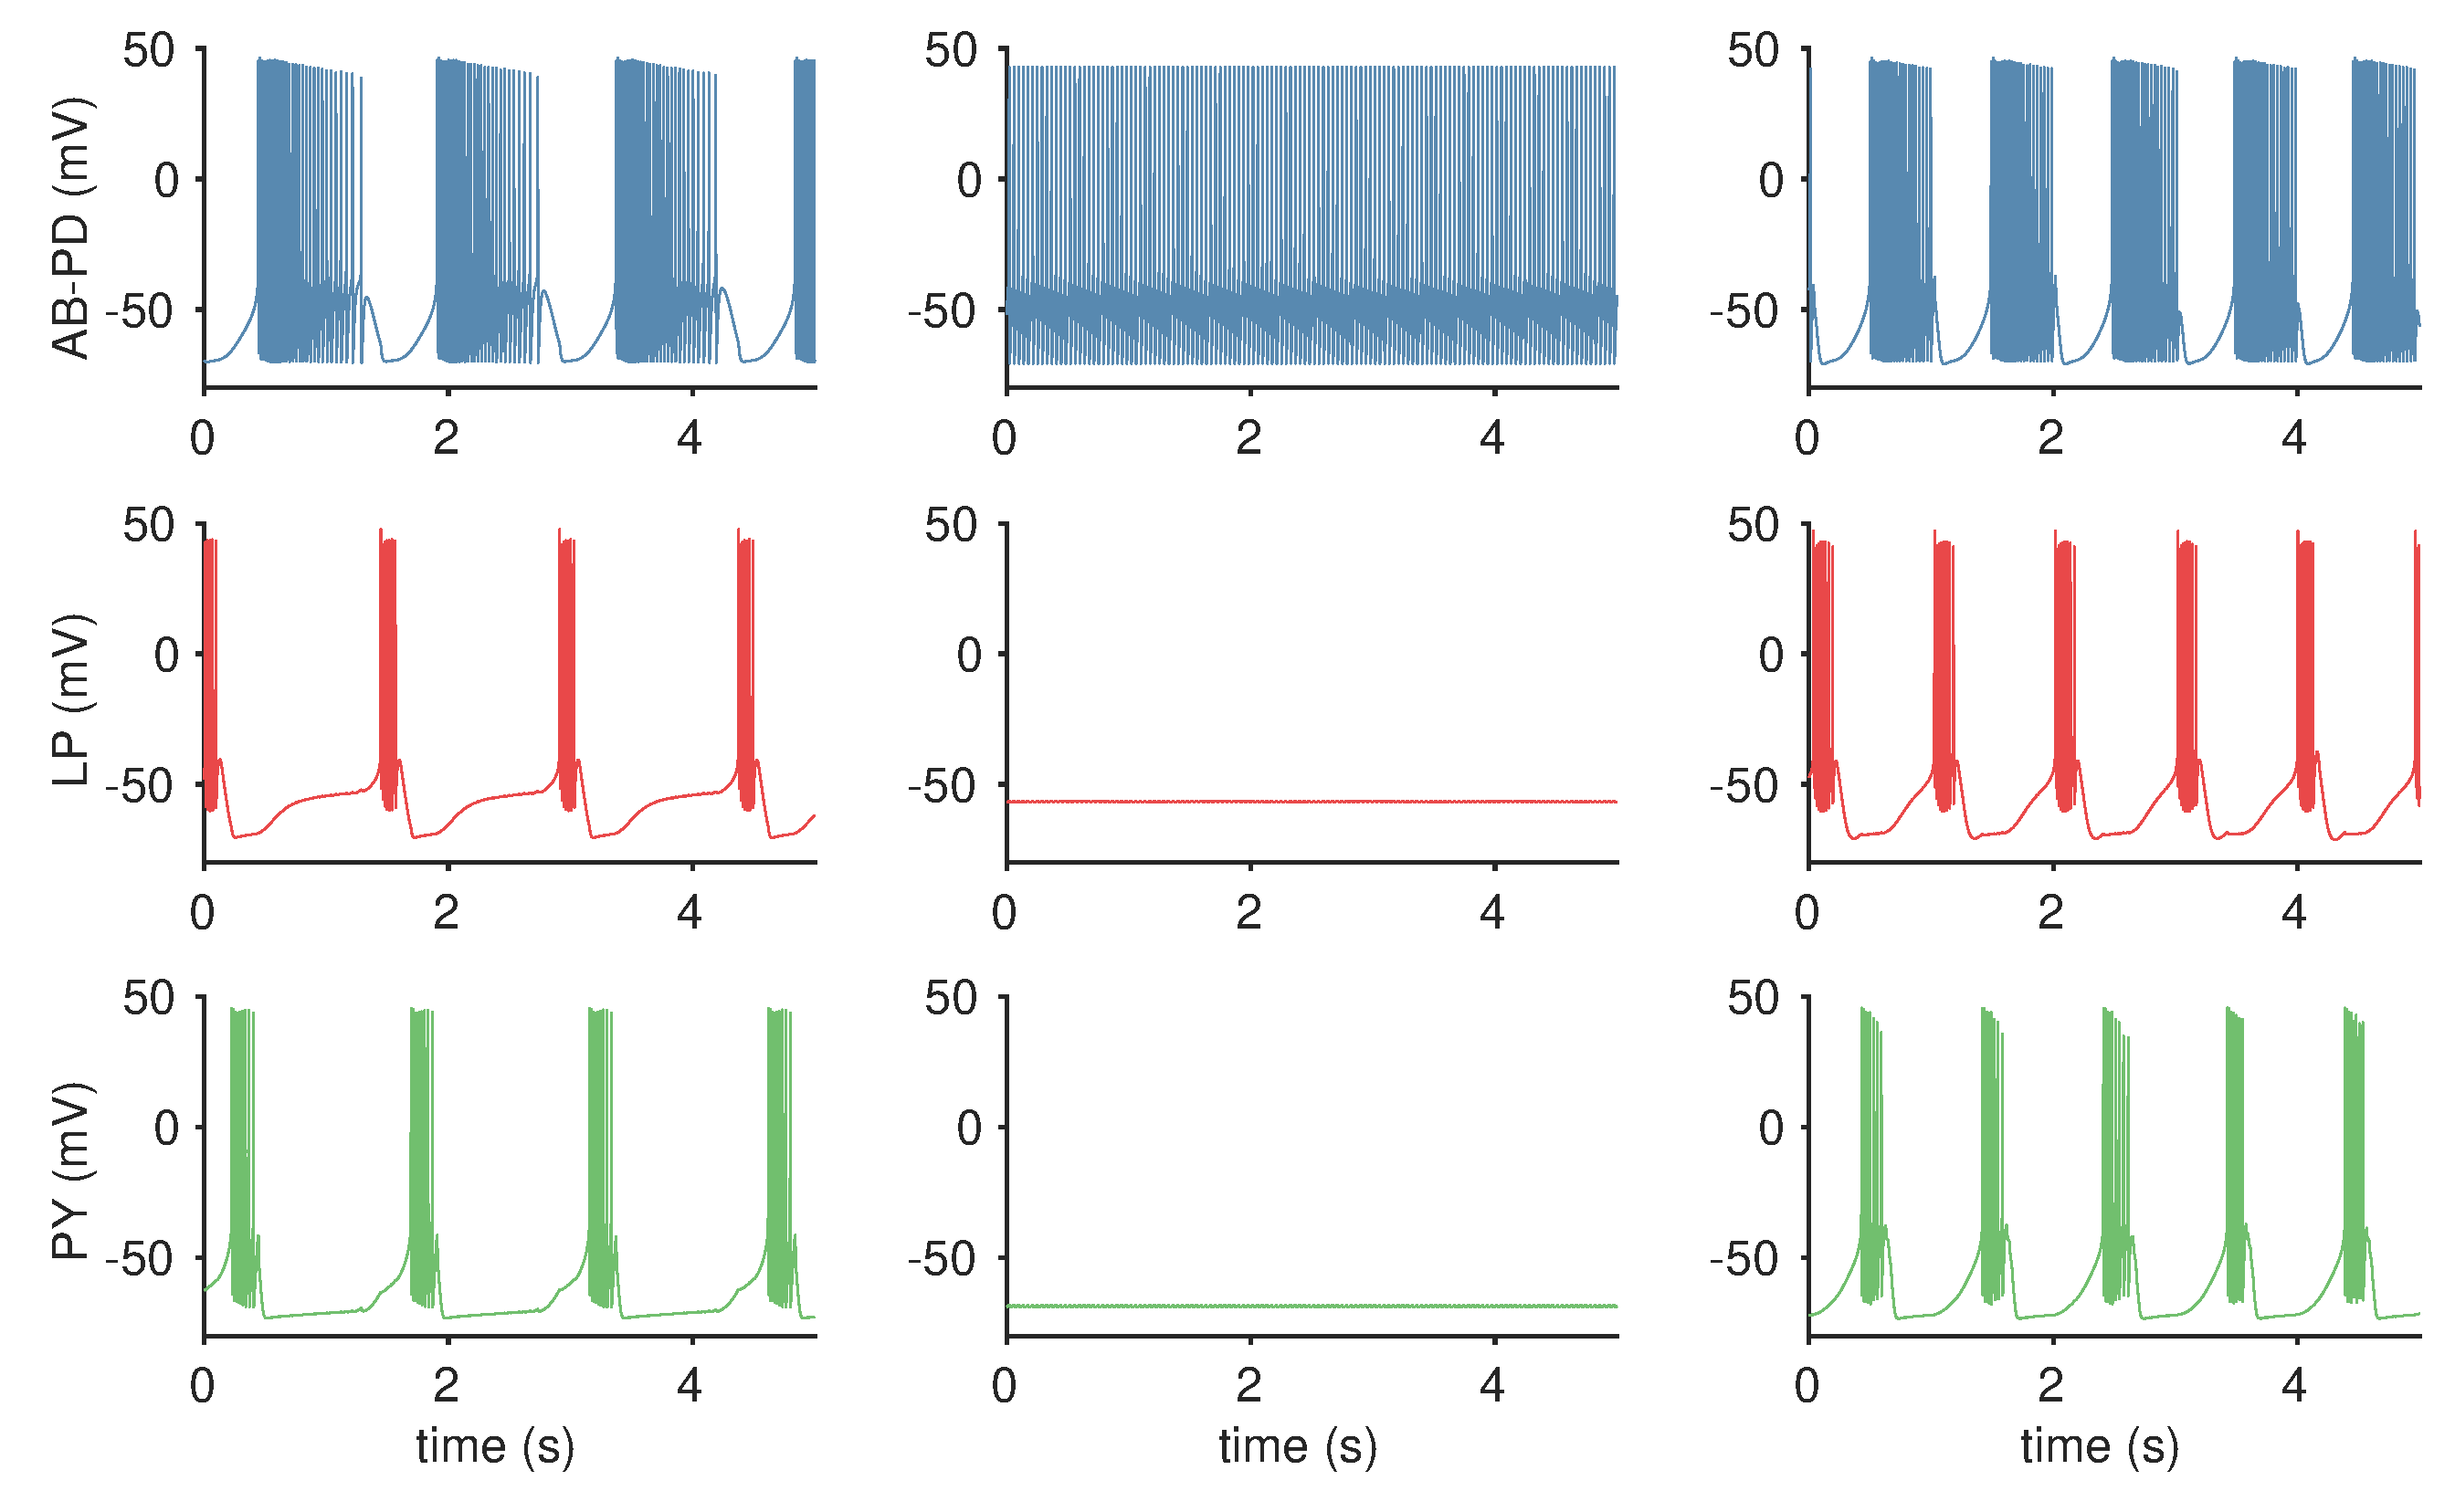
\includegraphics[width=1.0\linewidth]{gfx/all-modulation/traces4}
	\caption[Modulation of AB-PD can elicit tonic spiking (traces)]{Neuromodulation of \acs{AB}-\acs{PD} can depolarize \acs{AB}-\acs{PD}. Cells in columns are in the same network. \textit{Left:} No neuromodulation and a normal triphasic rhythm. \textit{Middle:} $\bar{g}_{MI}^{AB-PD} = 0.6~\mu \mathrm{S/mm^2}$, \acs{AB}-\acs{PD} is tonically spiking. \textit{Right:} Normal triphasic rhythm, where $\bar{g}_{MI}^{LP} = \bar{g}_{MI}^{AB-PD} = 1.0~\mu \mathrm{S/mm^2}$, normal triphasic rhythm with increased frequency.}
	\label{fig:traces4}
\end{figure}

\begin{figure}[b]
	\centering
	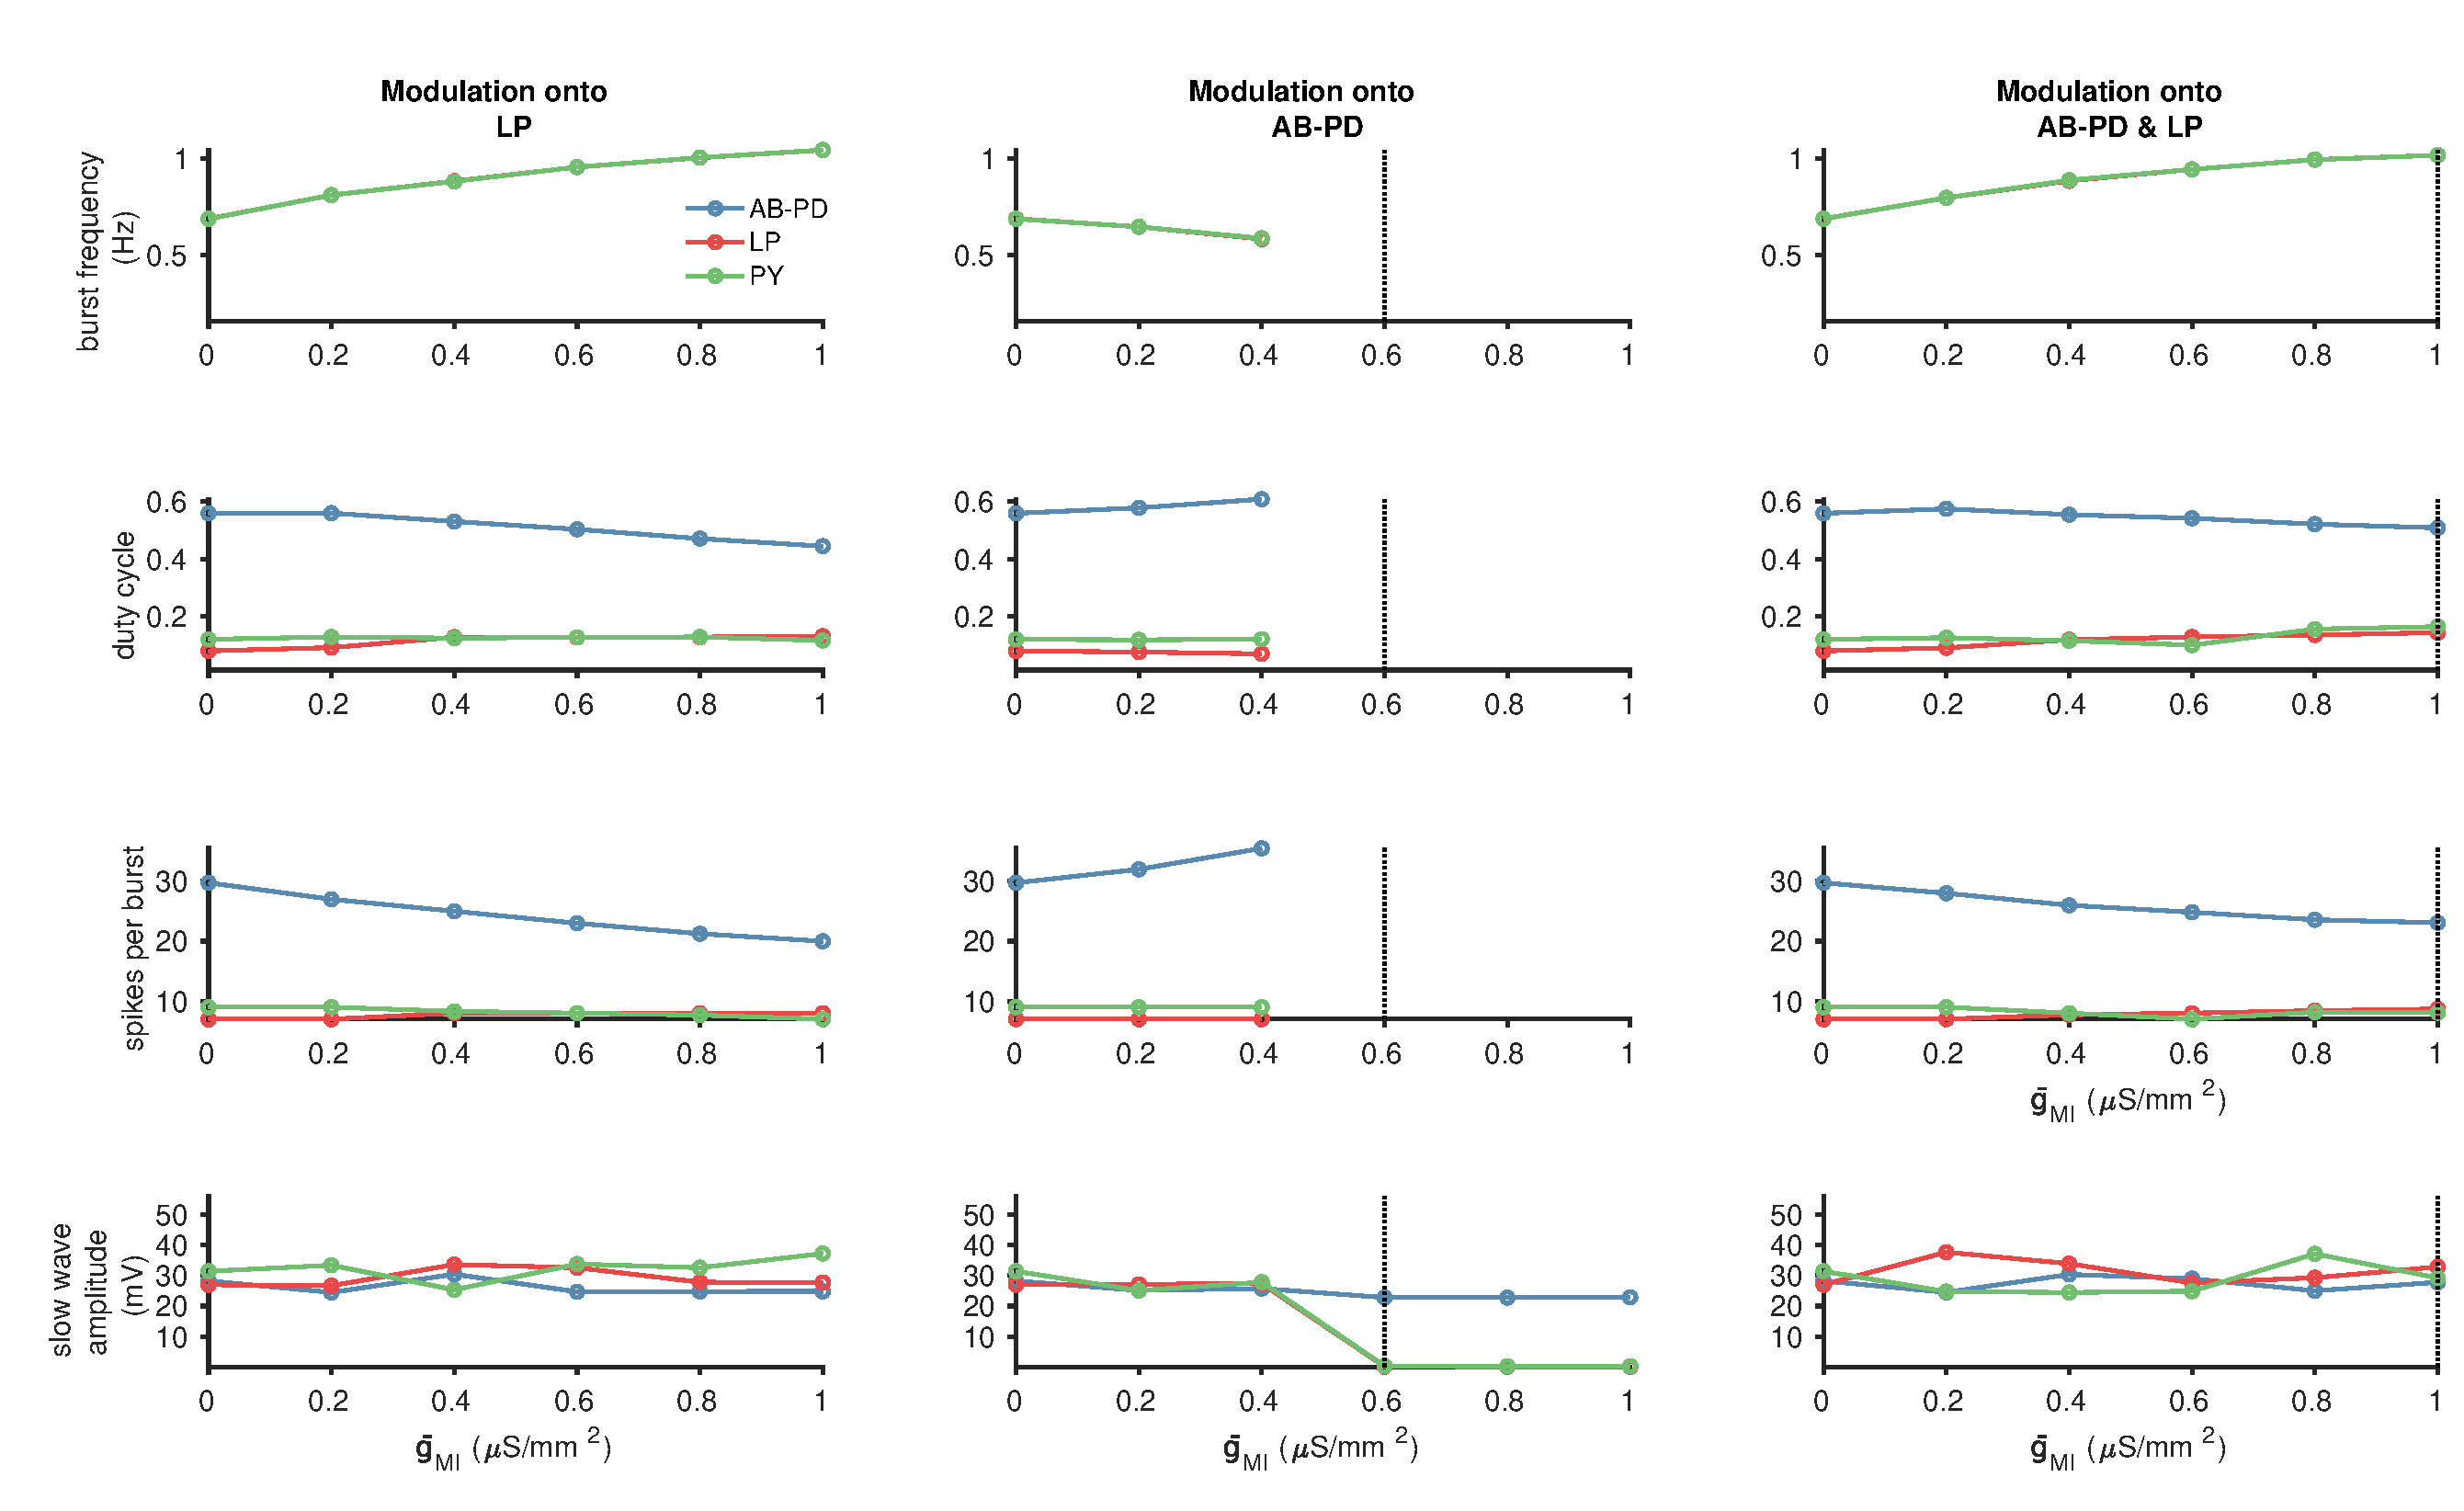
\includegraphics[width=1.0\linewidth]{gfx/all-modulation/metrics4}
	\caption[Modulation of AB-PD can elecit tonic spiking (metrics)]{Neuromodulation of the pacemaker model can result in tonic spiking. Modulation of LP offsets this effect, resulting in triphasic activity with increased frequency and amplitude with respect to the decentralized condition.}
	\label{fig:metrics4}
\end{figure}


%*****************************************
%*****************************************
%*****************************************
%*****************************************
%*****************************************

%\include{multiToC} % <--- just debug stuff, ignore for your documents
% ********************************************************************
% Backmatter
%*******************************************************
\appendix
%\renewcommand{\thechapter}{\alph{chapter}}
\cleardoublepage
\part{Appendix}
%********************************************************************
% Appendix
%*******************************************************
% If problems with the headers: get headings in appendix etc. right
%\markboth{\spacedlowsmallcaps{Appendix}}{\spacedlowsmallcaps{Appendix}}
\chapter{Appendix}

\section{Maximal Conductances for Model Neurons}
The dynamics and compartment parameters of each model neuron are described in \autoref{ch:methods}. The maximal conductances are as follows

\begin{table}[h]
	\myfloatalign
	\begin{tabularx}{\textwidth}{ccc} \toprule
		\tableheadline{Current} & $\bar{g}~(\mu\mathrm{S/mm^2})$ & \tableheadline{Notes}\\ \midrule
		\acs{IA} & 1844 & \\
		\acs{ICaS} & 103 & \\
		\acs{IH} & 0.39 &\\
		\acs{IKCa} & 214 & \\
		\acs{IKd} & 1746.96 & \\
		\acs{IMI} & 1 & 0 in the decentralized case \\ \bottomrule
	\end{tabularx}
	\caption{Maximal conductances for \autoref{fig:abwmod}.}
	\label{tab:appendix1}
\end{table}

\begin{table}[h]
	\myfloatalign
	\begin{tabularx}{\textwidth}{cccc} \toprule
		\tableheadline{Current} & \acs{AB}-\acs{PD} $\bar{g}~(\mu\mathrm{S/mm^2})$ & \acs{LP} $\bar{g}~(\mu\mathrm{S/mm^2})$ & \acs{PY} $\bar{g}~(\mu\mathrm{S/mm^2})$ \\ \midrule
		\acs{IA} & 483.25 & 341.98 & 449.88 \\
		\acs{ICaS} & 18.647 & 39.765 & 85.009 \\
		\acs{ICaT} & 30.368 & 14.649 & 9.9027 \\ 
		\acs{IH} & 0.14027 & 0.47477 & 0.3751 \\
		\acs{IKCa} & 99.998 & 88.89 & 14.637 \\
		\acs{IKd} & 1030.1 & 1093 & 1228.2 \\
		\acs{INa} & 1274.5 & 985.64 & 1797.1 \\ \bottomrule
	\end{tabularx}
	\caption{Maximal conductances for \autoref{fig:networkab47traces}.}
	\label{tab:appendix2ionic}
\end{table}

\begin{table}[h]
	\myfloatalign
	\begin{tabularx}{\textwidth}{cccc} \toprule
		\tableheadline{Current} & \tableheadline{Presynaptic} & \tableheadline{Postsynaptic} & $\bar{g}~(\mu\mathrm{S/mm^2})$ \\ \midrule
		\acs{Ichol} & AB-PD & LP & 59.724 \\
		\acs{Ichol} & AB-PD & PY & 94.508 \\
		\acs{Iglut} & AB-PD & LP & 79.803 \\ 
		\acs{Iglut} & AB-PD & PY & 97.881 \\
		\acs{Iglut} & LP & PY & 1.6985 \\
		\acs{Iglut} & PY & LP & 84.74 \\
		\acs{Iglut} & LP & AB-PD & 0.0128\\ \bottomrule
	\end{tabularx}
	\caption{Maximal conductances for \autoref{fig:networkab47traces}.}
	\label{tab:appendix2synaptic}
\end{table}

\begin{table}[h]
	\myfloatalign
	\begin{tabularx}{\textwidth}{cccc} \toprule
		\tableheadline{Current} & \acs{AB}-\acs{PD} $\bar{g}~(\mu\mathrm{S/mm^2})$ & \acs{LP} $\bar{g}~(\mu\mathrm{S/mm^2})$ & \acs{PY} $\bar{g}~(\mu\mathrm{S/mm^2})$ \\ \midrule
		\acs{IA} & 499.57 & 488.85 & 150.95 \\
		\acs{ICaS} & 42.16 & 5.9231 & 100 \\
		\acs{ICaT} & 29.236 & 48.989 & 0.00081 \\ 
		\acs{IH} & 0.3182 & 0.3666 & 0.1264 \\
		\acs{IKCa} & 100 & 62.559 & 99.359 \\
		\acs{IKd} & 878.65 & 911.94 & 816.2 \\
		\acs{INa} & 990.11 & 1733.6 & 1926.2 \\ \bottomrule
	\end{tabularx}
	\caption{Maximal conductances for \autoref{fig:networklp28traces}.}
	\label{tab:appendix3ionic}
\end{table}

\begin{table}[h]
	\myfloatalign
	\begin{tabularx}{\textwidth}{cccc} \toprule
		\tableheadline{Current} & \tableheadline{Presynaptic} & \tableheadline{Postsynaptic} & $\bar{g}~(\mu\mathrm{S/mm^2})$ \\ \midrule
		\acs{Ichol} & AB-PD & LP & 43.589 \\
		\acs{Ichol} & AB-PD & PY & 91.146 \\
		\acs{Iglut} & AB-PD & LP & 46.6953 \\ 
		\acs{Iglut} & AB-PD & PY & 71.918 \\
		\acs{Iglut} & LP & PY & 7.2045 \\
		\acs{Iglut} & PY & LP & 4.0693 \\
		\acs{Iglut} & LP & AB-PD & 43.899 \\ \bottomrule
	\end{tabularx}
	\caption{Maximal conductances for \autoref{fig:networklp28traces}.}
	\label{tab:appendix3synaptic}
\end{table}

\begin{table}[h]
	\myfloatalign
	\begin{tabularx}{\textwidth}{cccc} \toprule
		\tableheadline{Current} & \acs{AB}-\acs{PD} $\bar{g}~(\mu\mathrm{S/mm^2})$ & \acs{LP} $\bar{g}~(\mu\mathrm{S/mm^2})$ & \acs{PY} $\bar{g}~(\mu\mathrm{S/mm^2})$ \\ \midrule
		\acs{IA} & 384.09 & 215.15 & 398.88 \\
		\acs{ICaS} & 4.7276 & 21.739 & 91.294 \\
		\acs{ICaT} & 40.901 & 55.179 & 4.7064 \\ 
		\acs{IH} & 0.26391 & 0.48577 & 0.49937 \\
		\acs{IKCa} & 56.614 & 83.753 & 6.9534 \\
		\acs{IKd} & 766.44 &   1196 & 1103.7 \\
		\acs{INa} & 1719.3 & 1791.4 & 1978.6  \\ \bottomrule
	\end{tabularx}
	\caption{Maximal conductances for \autoref{fig:networkablp14traces}.}
	\label{tab:appendix4ionic}
\end{table}

\begin{table}[h]
	\myfloatalign
	\begin{tabularx}{\textwidth}{cccc} \toprule
		\tableheadline{Current} & \tableheadline{Presynaptic} & \tableheadline{Postsynaptic} & $\bar{g}~(\mu\mathrm{S/mm^2})$ \\ \midrule
		\acs{Ichol} & AB-PD & LP & 0.70694 \\
		\acs{Ichol} & AB-PD & PY & 2.5239 \\
		\acs{Iglut} & AB-PD & LP & 14.382 \\ 
		\acs{Iglut} & AB-PD & PY & 96.992 \\
		\acs{Iglut} & LP & PY & 22.72 \\
		\acs{Iglut} & PY & LP & 16.11 \\
		\acs{Iglut} & LP & AB-PD & 54.05 \\ \bottomrule
	\end{tabularx}
	\caption{Maximal conductances for \autoref{fig:networkablp14traces}.}
	\label{tab:appendix4synaptic}
\end{table}

\begin{table}[h]
	\myfloatalign
	\begin{tabularx}{\textwidth}{cccc} \toprule
		\tableheadline{Current} & \acs{AB}-\acs{PD} $\bar{g}~(\mu\mathrm{S/mm^2})$ & \acs{LP} $\bar{g}~(\mu\mathrm{S/mm^2})$ & \acs{PY} $\bar{g}~(\mu\mathrm{S/mm^2})$ \\ \midrule
		\acs{IA} & 48.274  & 486.59 &  361.85 \\
		\acs{ICaS} & 0.95921 &  52.628 &  35.453 \\
		\acs{ICaT} & 44.247 &  31.541 &  58.985 \\ 
		\acs{IH} & 0.057166 & 0.42321 & 0.42576 \\
		\acs{IKCa} & 63.068 &  93.046 & 54 \\
		\acs{IKd} & 957.19 &  1075.4 &  1153.9 \\
		\acs{INa} & 1584.4 &  1196.8 &  1835.9  \\ \bottomrule
	\end{tabularx}
	\caption{Maximal conductances for \autoref{fig:traces1}.}
	\label{tab:appendix5ionic}
\end{table}

\begin{table}[h]
	\myfloatalign
	\begin{tabularx}{\textwidth}{cccc} \toprule
		\tableheadline{Current} & \tableheadline{Presynaptic} & \tableheadline{Postsynaptic} & $\bar{g}~(\mu\mathrm{S/mm^2})$ \\ \midrule
		\acs{Ichol} & AB-PD & LP & 21.247 \\
		\acs{Ichol} & AB-PD & PY & 17.497 \\
		\acs{Iglut} & AB-PD & LP & 92.692 \\ 
		\acs{Iglut} & AB-PD & PY & 74.007 \\
		\acs{Iglut} & LP & PY & 97.419 \\
		\acs{Iglut} & PY & LP & 93.541 \\
		\acs{Iglut} & LP & AB-PD & 51.799 \\ \bottomrule
	\end{tabularx}
	\caption{Maximal conductances for \autoref{fig:traces1}.}
	\label{tab:appendix5synaptic}
\end{table}

\begin{table}[h]
	\myfloatalign
	\begin{tabularx}{\textwidth}{cccc} \toprule
		\tableheadline{Current} & \acs{AB}-\acs{PD} $\bar{g}~(\mu\mathrm{S/mm^2})$ & \acs{LP} $\bar{g}~(\mu\mathrm{S/mm^2})$ & \acs{PY} $\bar{g}~(\mu\mathrm{S/mm^2})$ \\ \midrule
		\acs{IA} & 9.5645 & 0 & 67.751 \\
		\acs{ICaS} & 6.8258 & 30.335 & 32.357 \\
		\acs{ICaT} & 27.819   &   0.12634 & 5.7595 \\ 
		\acs{IH} & 0.029794   &   0.38326 &     0.26788 \\
		\acs{IKCa} & 82.919 & 85.903 &  49.91 \\
		\acs{IKd} & 1180.3 & 254.78 & 1188.6 \\
		\acs{INa} & 1934 & 1707.7 & 1895.7  \\ \bottomrule
	\end{tabularx}
	\caption{Maximal conductances for \autoref{fig:traces2}.}
	\label{tab:appendix6ionic}
\end{table}

\begin{table}[h]
	\myfloatalign
	\begin{tabularx}{\textwidth}{cccc} \toprule
		\tableheadline{Current} & \tableheadline{Presynaptic} & \tableheadline{Postsynaptic} & $\bar{g}~(\mu\mathrm{S/mm^2})$ \\ \midrule
		\acs{Ichol} & AB-PD & LP & 18.975 \\
		\acs{Ichol} & AB-PD & PY & 100 \\
		\acs{Iglut} & AB-PD & LP & 15.721 \\ 
		\acs{Iglut} & AB-PD & PY & 19.862 \\
		\acs{Iglut} & LP & PY & 27.179 \\
		\acs{Iglut} & PY & LP & 63.191 \\
		\acs{Iglut} & LP & AB-PD & 59.59 \\ \bottomrule
	\end{tabularx}
	\caption{Maximal conductances for \autoref{fig:traces2}.}
	\label{tab:appendix6synaptic}
\end{table}

\begin{table}[h]
	\myfloatalign
	\begin{tabularx}{\textwidth}{cccc} \toprule
		\tableheadline{Current} & \acs{AB}-\acs{PD} $\bar{g}~(\mu\mathrm{S/mm^2})$ & \acs{LP} $\bar{g}~(\mu\mathrm{S/mm^2})$ & \acs{PY} $\bar{g}~(\mu\mathrm{S/mm^2})$ \\ \midrule
		\acs{IA} & 142.64 & 280.07 & 20.373 \\
		\acs{ICaS} & 53.39 &  31.45 & 14.268 \\
		\acs{ICaT} & 7.0457 & 36.037 & 53.337 \\ 
		\acs{IH} & 0.11766   &   0.49646   &   0.37665 \\
		\acs{IKCa} & 87.08 & 84.953 & 20.246 \\
		\acs{IKd} & 782.28 & 718.61 & 1026.5 \\
		\acs{INa} & 1846 & 1702.4 & 1998.7  \\ \bottomrule
	\end{tabularx}
	\caption{Maximal conductances for \autoref{fig:traces3}.}
	\label{tab:appendix7ionic}
\end{table}

\begin{table}[h]
	\myfloatalign
	\begin{tabularx}{\textwidth}{cccc} \toprule
		\tableheadline{Current} & \tableheadline{Presynaptic} & \tableheadline{Postsynaptic} & $\bar{g}~(\mu\mathrm{S/mm^2})$ \\ \midrule
		\acs{Ichol} & AB-PD & LP & 0.001 \\
		\acs{Ichol} & AB-PD & PY & 84.207 \\
		\acs{Iglut} & AB-PD & LP & 5.7983 \\ 
		\acs{Iglut} & AB-PD & PY & 1.6739 \\
		\acs{Iglut} & LP & PY & 95.435 \\
		\acs{Iglut} & PY & LP & 7.7081 \\
		\acs{Iglut} & LP & AB-PD &  97.889 \\ \bottomrule
	\end{tabularx}
	\caption{Maximal conductances for \autoref{fig:traces3}.}
	\label{tab:appendix8ionic}
\end{table}

\begin{table}[h]
	\myfloatalign
	\begin{tabularx}{\textwidth}{cccc} \toprule
		\tableheadline{Current} & \acs{AB}-\acs{PD} $\bar{g}~(\mu\mathrm{S/mm^2})$ & \acs{LP} $\bar{g}~(\mu\mathrm{S/mm^2})$ & \acs{PY} $\bar{g}~(\mu\mathrm{S/mm^2})$ \\ \midrule
		\acs{IA} & 103.45 &  464.2 & 458.17 \\
		\acs{ICaS} & 62.458 & 28.521 & 64.549 \\
		\acs{ICaT} & 3.2673 & 39.564 & 6.7024 \\ 
		\acs{IH} & 0.41882   &   0.41944   &   0.39775 \\
		\acs{IKCa} & 99.338 & 87.122 & 68.104 \\
		\acs{IKd} & 1242.4 &   1023 & 1245.5 \\
		\acs{INa} & 1343.2 & 1862.4 & 1693.5  \\ \bottomrule
	\end{tabularx}
	\caption{Maximal conductances for \autoref{fig:traces4}.}
	\label{tab:appendix9ionic}
\end{table}

\begin{table}[h]
	\myfloatalign
	\begin{tabularx}{\textwidth}{cccc} \toprule
		\tableheadline{Current} & \tableheadline{Presynaptic} & \tableheadline{Postsynaptic} & $\bar{g}~(\mu\mathrm{S/mm^2})$ \\ \midrule
		\acs{Ichol} & AB-PD & LP & 0.019872 \\
		\acs{Ichol} & AB-PD & PY & 24.633 \\
		\acs{Iglut} & AB-PD & LP & 4.1505 \\ 
		\acs{Iglut} & AB-PD & PY & 60.444 \\
		\acs{Iglut} & LP & PY & 10.058 \\
		\acs{Iglut} & PY & LP & 69.451 \\
		\acs{Iglut} & LP & AB-PD &  65.046 \\ \bottomrule
	\end{tabularx}
	\caption{Maximal conductances for \autoref{fig:traces4}.}
	\label{tab:appendix10ionic}
\end{table}

\FloatBarrier

\section{Supplemental Figures}

\begin{figure}[h]
	\centering
	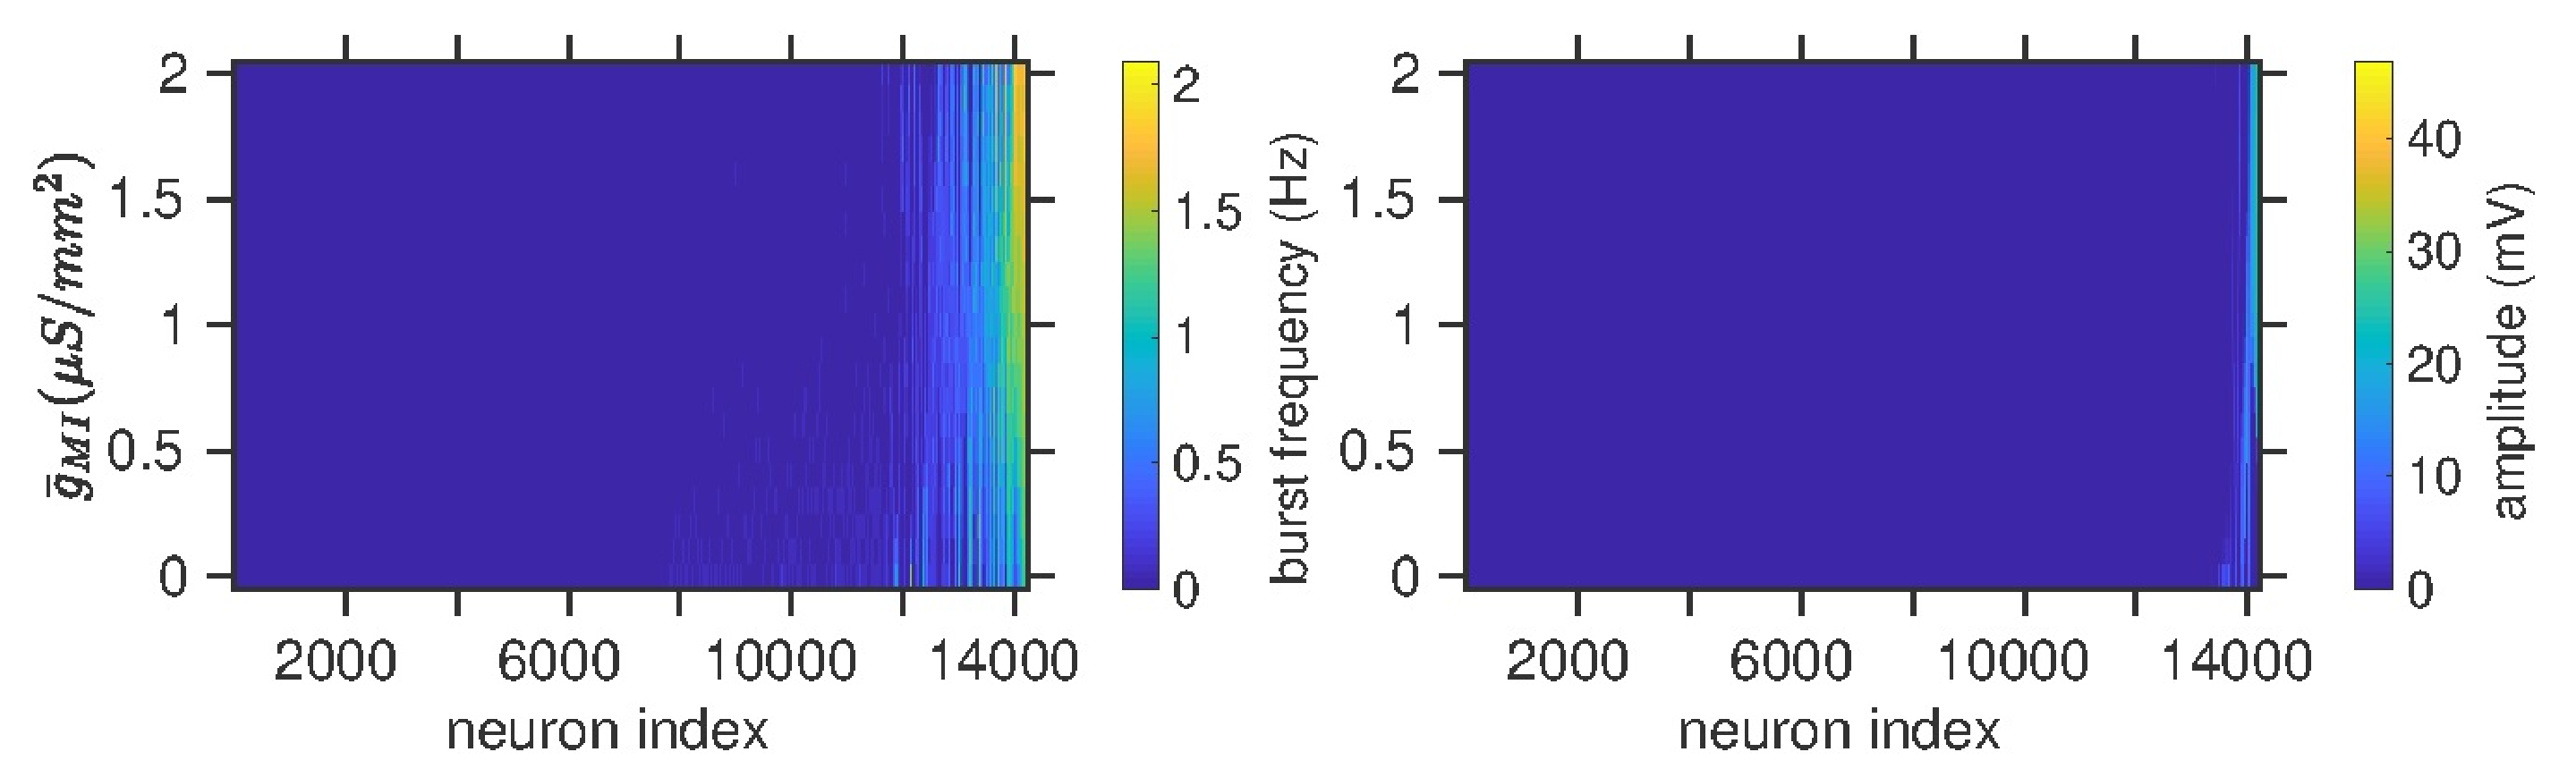
\includegraphics[width=1.0\linewidth]{gfx/prinz-models/prinz}
	\caption[Database models with modulatory input]{Database models without \acs{INa} or \acs{ICaT} with modulatory input respond over a small range of maximal conductance. Most database models do not respond to modulatory input. A subset increase in frequency and amplitude (peak voltage - trough voltage). Models are sorted by mean metric value.}
	\label{fig:prinzburstingmodelsnavcatswensen}
\end{figure}

\begin{figure}[h]
	\centering
	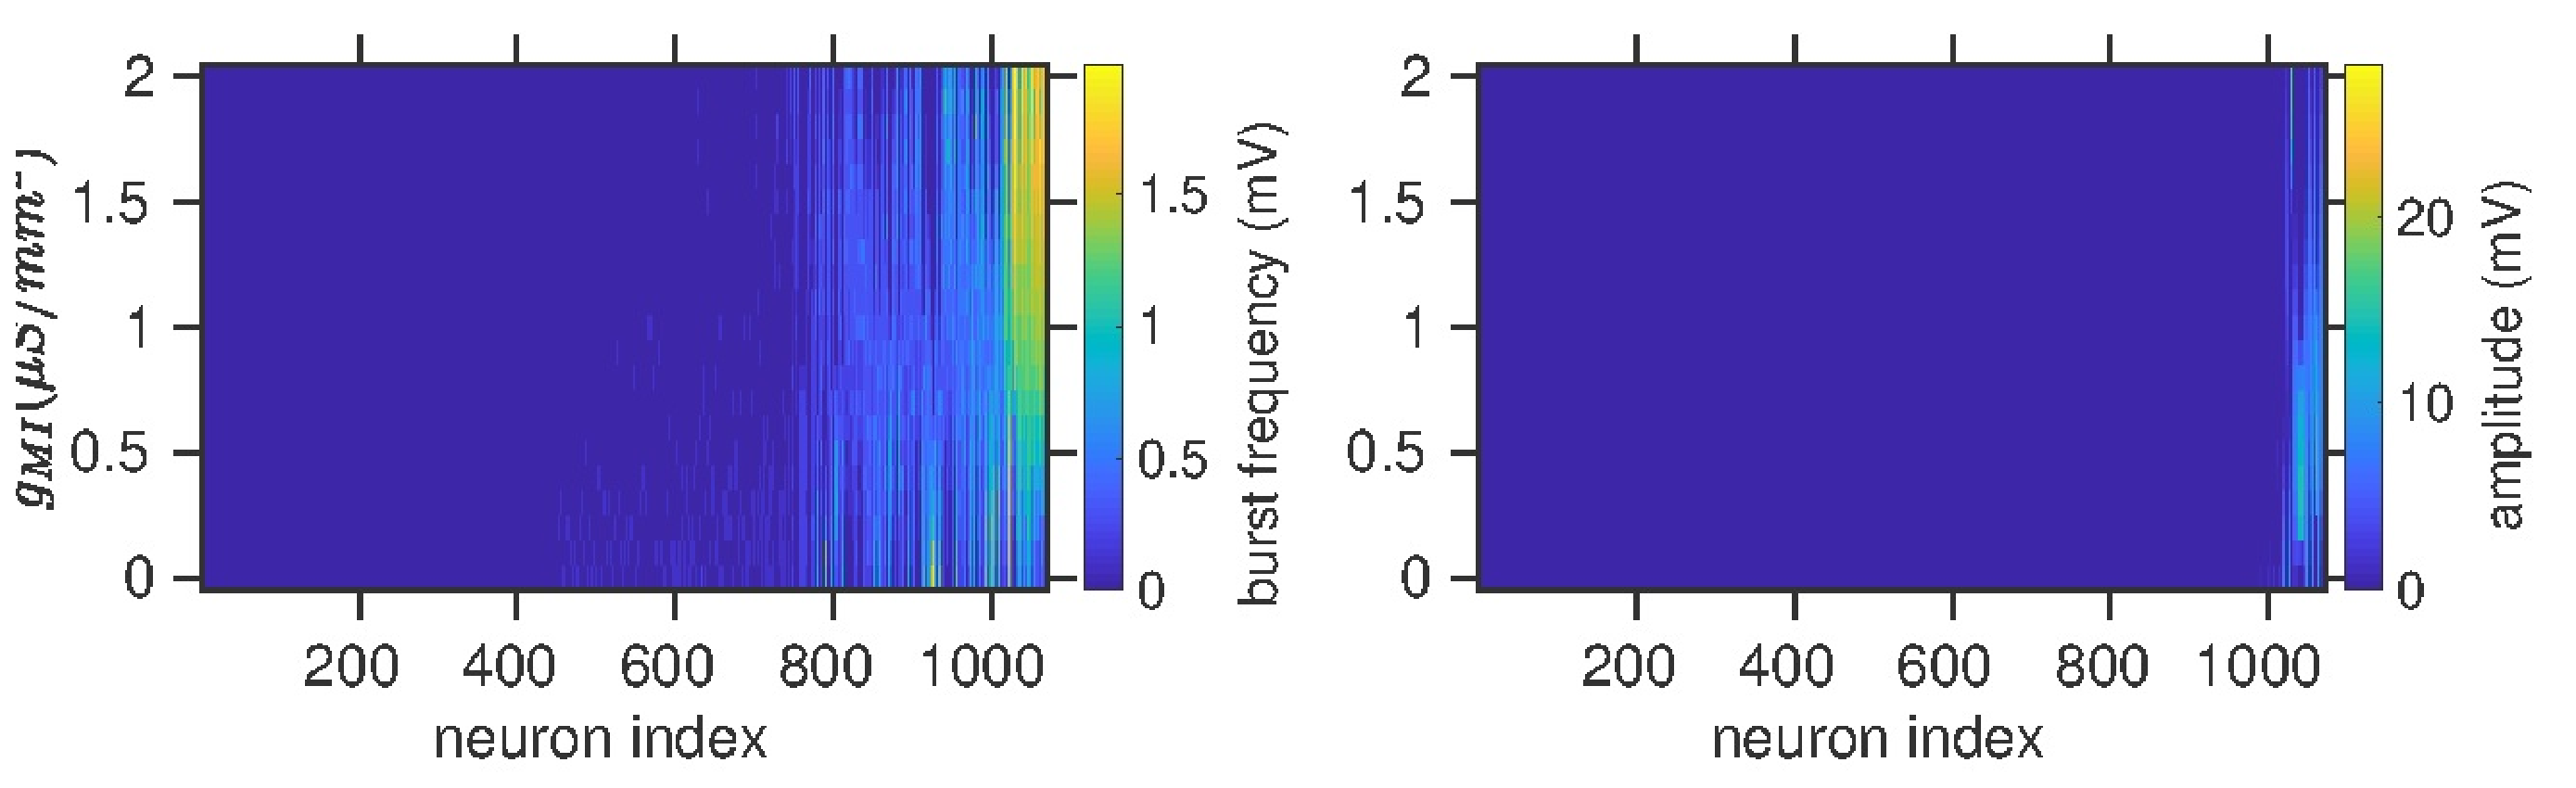
\includegraphics[width=1.0\linewidth]{gfx/prinz-models/prinz_excised}
	\caption[Responsive database models with modulatory input]{A subset of database models with \acs{INa} or \acs{ICaT} were responsive to modulatory input. The 1000 models with the greatest change in frequency and amplitude were plotted with updated color scaling. Models are sorted by mean metric value.}
	\label{fig:prinzburstingmodelsnavcatexcisedswensen}
\end{figure}

\begin{figure}
	\centering
	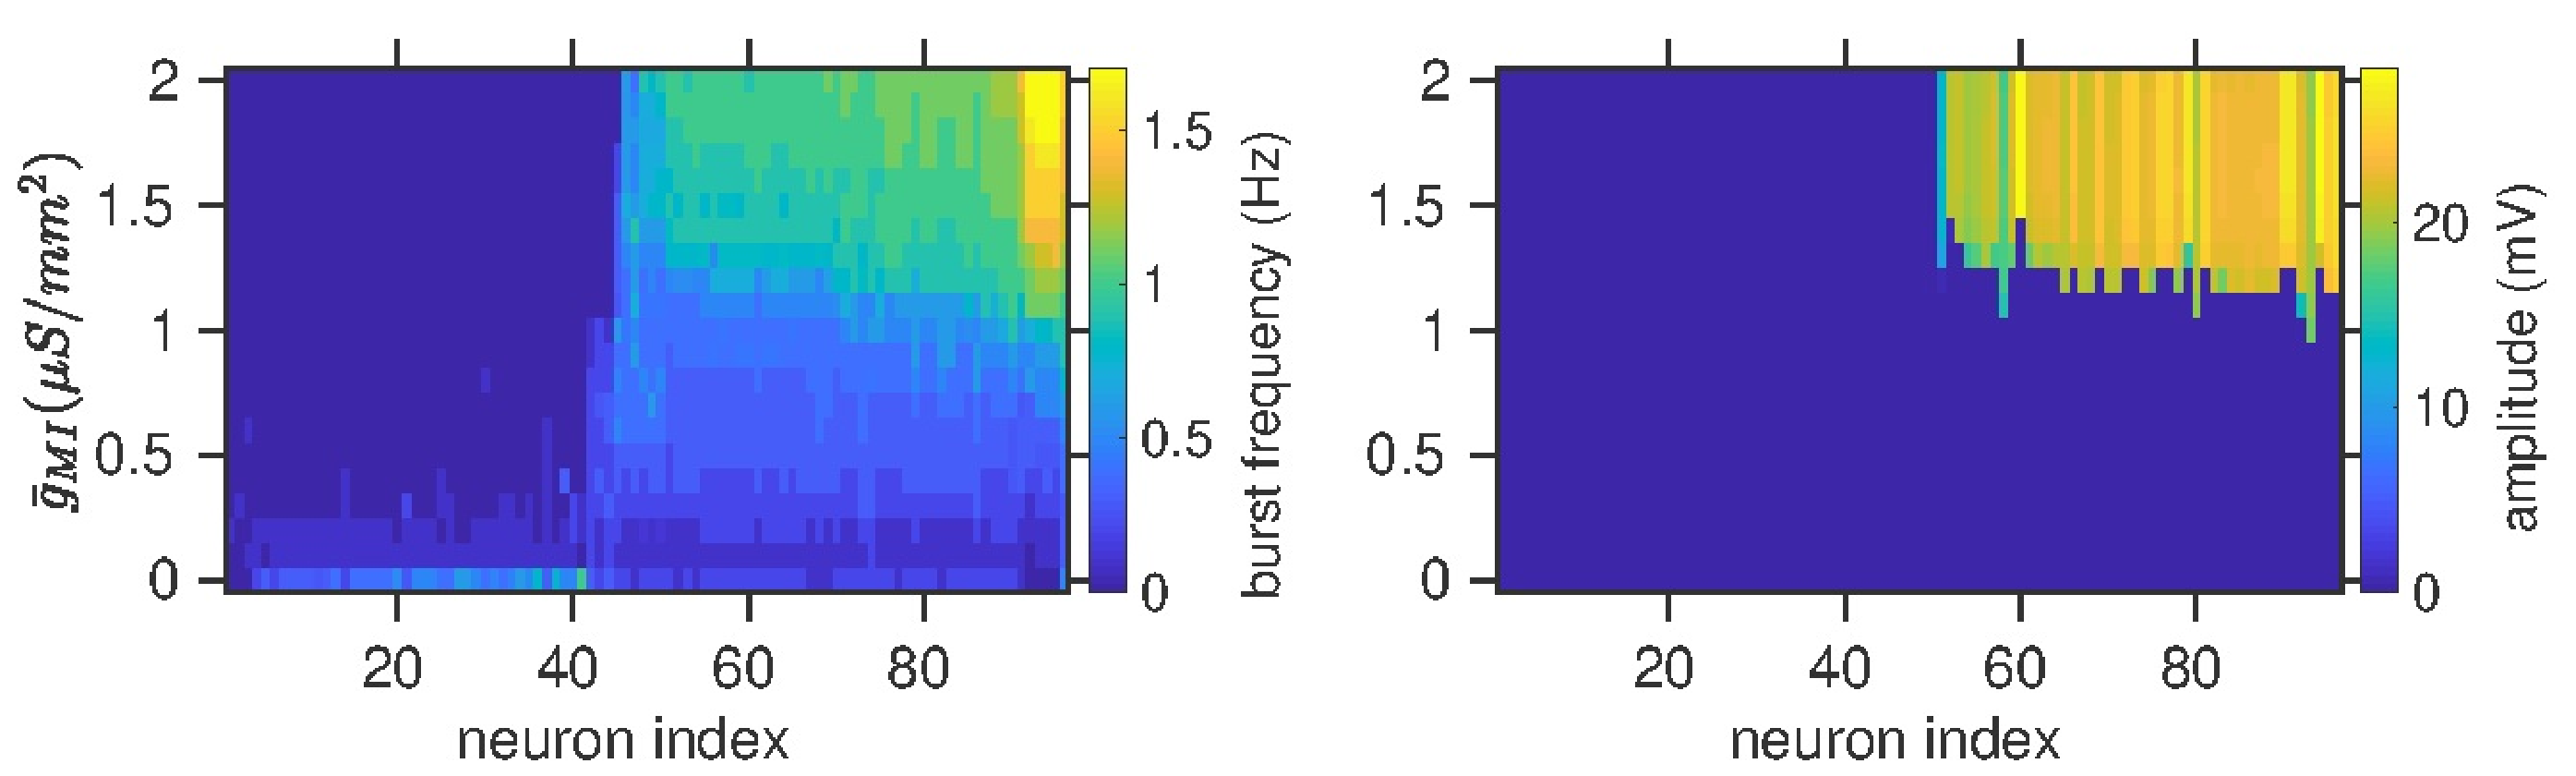
\includegraphics[width=1.0\linewidth]{gfx/prinz-models/prinz_optimized}
	\caption[Optimized database models increase in frequency and amplitude]{Models optimized for a graded increase in frequency and amplitude under increasing modulatory input experience frequency as a graded transition and amplitude as a switch between quiescence and high amplitude. Optimized models display graded increase in burst frequency as the maximal conductance of modulatory input increases. Amplitude increases sharply during a transitional state as maximal conductance of \acs{IMI} increases. Models are sorted by mean metric value.}
	\label{fig:figprinzburstingttxcatnoscgmiswensenexprosim3}
\end{figure}

\begin{figure}
	\centering
	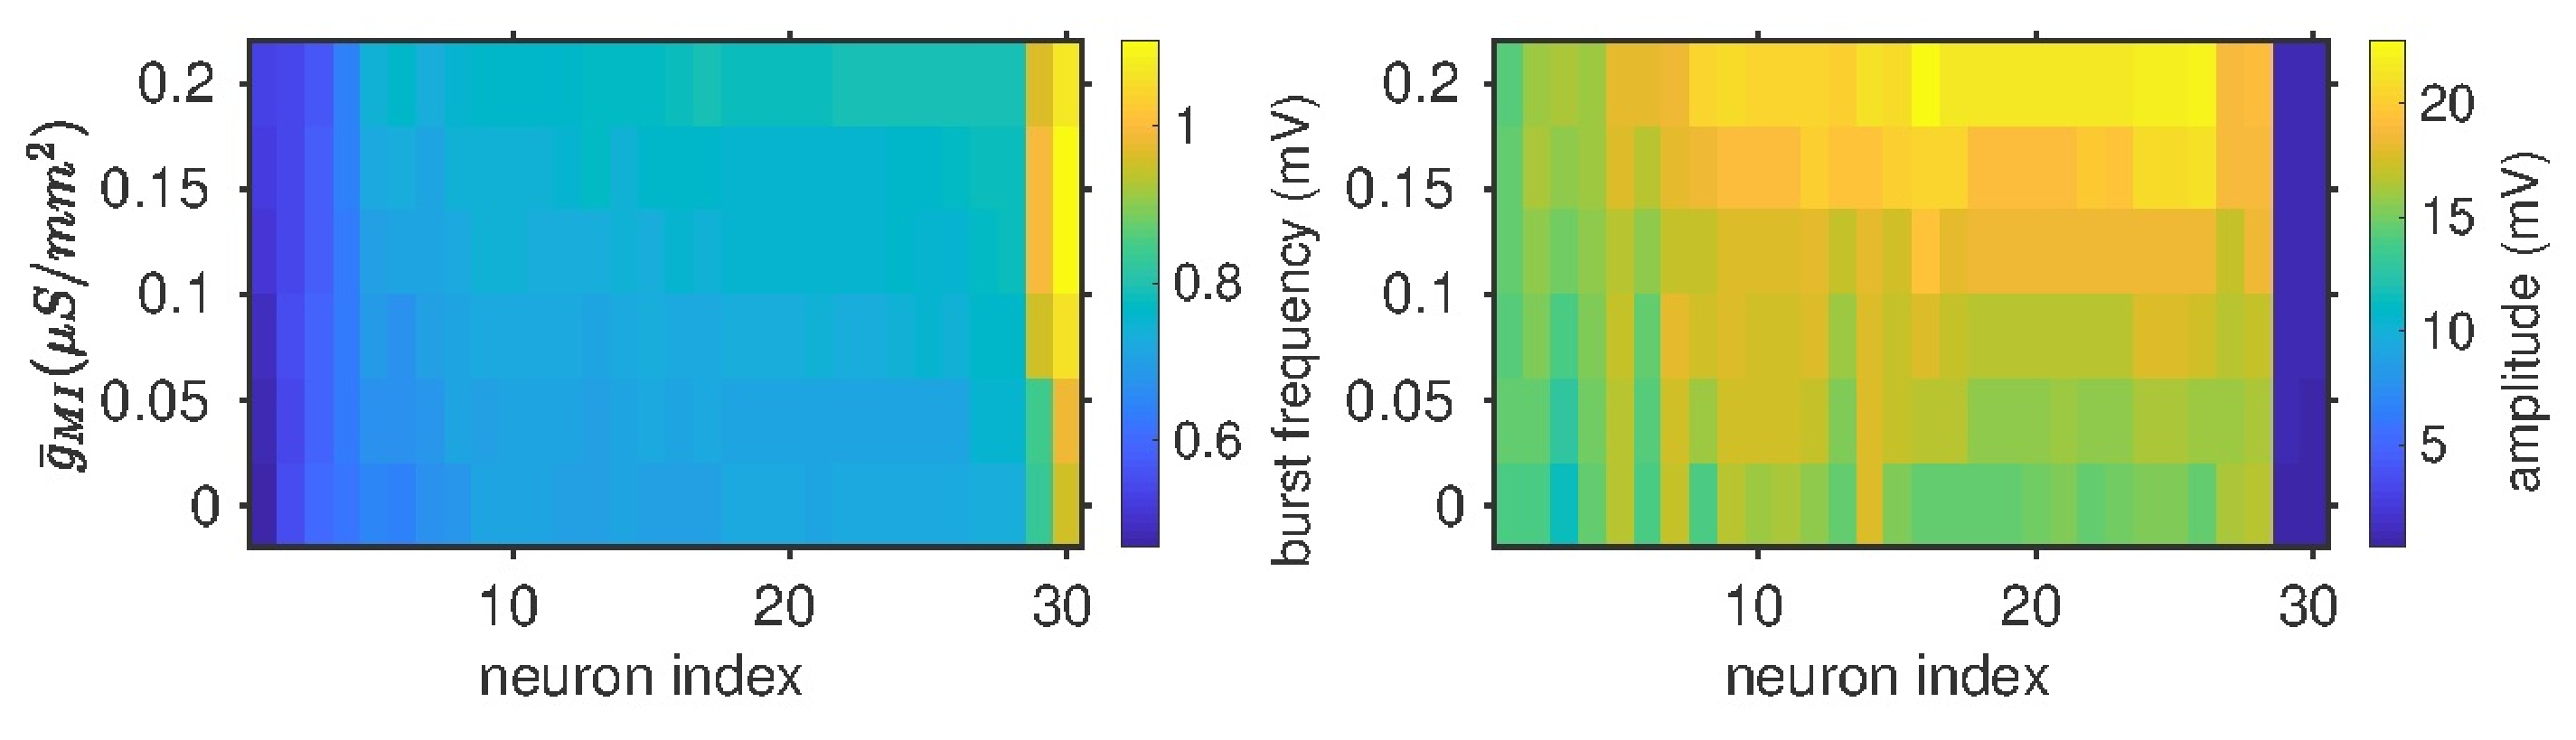
\includegraphics[width=1.0\linewidth]{gfx/prinz-models/plot_optim_AB_graded}
	\caption[Optimized database models smoothly increase in frequency and amplitude]{Models optimized for a graded increase in burst frequency and amplitude over increasing modulatory input. Modulatory input increases the amplitude of slow-wave oscillations by increasing the peak voltage. In these models, the duty cycle remains constant and the frequency increases.}
	\label{fig:plotoptimabgraded}
\end{figure}


%********************************************************************
% Other Stuff in the Back
%*******************************************************
\cleardoublepage%********************************************************************
% Bibliography
%*******************************************************
% work-around to have small caps also here in the headline
% https://tex.stackexchange.com/questions/188126/wrong-header-in-bibliography-classicthesis
% Thanks to Enrico Gregorio
\defbibheading{bibintoc}[\bibname]{%
  \phantomsection
  \manualmark
  \markboth{\spacedlowsmallcaps{#1}}{\spacedlowsmallcaps{#1}}%
  \addtocontents{toc}{\protect\vspace{\beforebibskip}}%
  \addcontentsline{toc}{chapter}{\tocEntry{#1}}%
  \chapter*{#1}%
}
\printbibliography[heading=bibintoc]

% Old version, will be removed later
% work-around to have small caps also here in the headline
%\manualmark
%\markboth{\spacedlowsmallcaps{\bibname}}{\spacedlowsmallcaps{\bibname}} % work-around to have small caps also
%\phantomsection
%\refstepcounter{dummy}
%\addtocontents{toc}{\protect\vspace{\beforebibskip}} % to have the bib a bit from the rest in the toc
%\addcontentsline{toc}{chapter}{\tocEntry{\bibname}}
%\label{app:bibliography}
%\printbibliography

\cleardoublepage%*******************************************************
% Declaration
%*******************************************************
\refstepcounter{dummy}
\pdfbookmark[0]{Declaration}{declaration}
\chapter*{Declaration}
\thispagestyle{empty}
I hereby certify that this thesis is entirely my own work. All code can be found at \url{https://gitlab.com/marderlab}.
\bigskip

\noindent\textit{\myLocation, \myTime}

\smallskip

\begin{flushright}
    \begin{tabular}{m{5cm}}
        \\ \hline
        \centering\myName \\
    \end{tabular}
\end{flushright}

\cleardoublepage\pagestyle{empty}

\hfill

\vfill


\pdfbookmark[0]{Colophon}{colophon}
\section*{Colophon}
This document was typeset using the typographical look-and-feel \texttt{classicthesis} developed by Andr\'e Miede and Ivo Pletikosić.
The style was inspired by Robert Bringhurst's seminal book on typography ``\emph{The Elements of Typographic Style}''.
\texttt{classicthesis} is available for both \LaTeX\ and \mLyX:
\begin{center}
\url{https://bitbucket.org/amiede/classicthesis/}
\end{center}
Happy users of \texttt{classicthesis} usually send a real postcard to the author, a collection of postcards received so far is featured here:
\begin{center}
\url{http://postcards.miede.de/}
\end{center}
Thank you very much for your feedback and contribution.

\bigskip

\noindent\finalVersionString

%Hermann Zapf's \emph{Palatino} and \emph{Euler} type faces (Type~1 PostScript fonts \emph{URW
%Palladio L} and \emph{FPL}) are used. The ``typewriter'' text is typeset in \emph{Bera Mono},
%originally developed by Bitstream, Inc. as ``Bitstream Vera''. (Type~1 PostScript fonts were made
%available by Malte Rosenau and
%Ulrich Dirr.)

%\paragraph{note:} The custom size of the textblock was calculated
%using the directions given by Mr. Bringhurst (pages 26--29 and
%175/176). 10~pt Palatino needs  133.21~pt for the string
%``abcdefghijklmnopqrstuvwxyz''. This yields a good line length between
%24--26~pc (288--312~pt). Using a ``\emph{double square textblock}''
%with a 1:2 ratio this results in a textblock of 312:624~pt (which
%includes the headline in this design). A good alternative would be the
%``\emph{golden section textblock}'' with a ratio of 1:1.62, here
%312:505.44~pt. For comparison, \texttt{DIV9} of the \texttt{typearea}
%package results in a line length of 389~pt (32.4~pc), which is by far
%too long. However, this information will only be of interest for
%hardcore pseudo-typographers like me.%
%
%To make your own calculations, use the following commands and look up
%the corresponding lengths in the book:
%\begin{verbatim}
%    \settowidth{\abcd}{abcdefghijklmnopqrstuvwxyz}
%    \the\abcd\ % prints the value of the length
%\end{verbatim}
%Please see the file \texttt{classicthesis.sty} for some precalculated
%values for Palatino and Minion.
%
%    \settowidth{\abcd}{abcdefghijklmnopqrstuvwxyz}
%    \the\abcd\ % prints the value of the length

% ********************************************************************
% Game Over: Restore, Restart, or Quit?
%*******************************************************
\end{document}
% ********************************************************************
